% Options for packages loaded elsewhere
\PassOptionsToPackage{unicode}{hyperref}
\PassOptionsToPackage{hyphens}{url}
\documentclass[
]{article}
\usepackage{xcolor}
\usepackage{amsmath,amssymb}
\setcounter{secnumdepth}{-\maxdimen} % remove section numbering
\usepackage{iftex}
\ifPDFTeX
  \usepackage[T1]{fontenc}
  \usepackage[utf8]{inputenc}
  \usepackage{textcomp} % provide euro and other symbols
\else % if luatex or xetex
  \usepackage{unicode-math} % this also loads fontspec
  \defaultfontfeatures{Scale=MatchLowercase}
  \defaultfontfeatures[\rmfamily]{Ligatures=TeX,Scale=1}
\fi
\usepackage{lmodern}
\ifPDFTeX\else
  % xetex/luatex font selection
\fi
% Use upquote if available, for straight quotes in verbatim environments
\IfFileExists{upquote.sty}{\usepackage{upquote}}{}
\IfFileExists{microtype.sty}{% use microtype if available
  \usepackage[]{microtype}
  \UseMicrotypeSet[protrusion]{basicmath} % disable protrusion for tt fonts
}{}
\makeatletter
\@ifundefined{KOMAClassName}{% if non-KOMA class
  \IfFileExists{parskip.sty}{%
    \usepackage{parskip}
  }{% else
    \setlength{\parindent}{0pt}
    \setlength{\parskip}{6pt plus 2pt minus 1pt}}
}{% if KOMA class
  \KOMAoptions{parskip=half}}
\makeatother
\usepackage{listings}
\newcommand{\passthrough}[1]{#1}
\lstset{defaultdialect=[5.3]Lua}
\lstset{defaultdialect=[x86masm]Assembler}
\usepackage{longtable,booktabs,array}
\newcounter{none} % for unnumbered tables
\usepackage{multirow}
\usepackage{calc} % for calculating minipage widths
% Correct order of tables after \paragraph or \subparagraph
\usepackage{etoolbox}
\makeatletter
\patchcmd\longtable{\par}{\if@noskipsec\mbox{}\fi\par}{}{}
\makeatother
% Allow footnotes in longtable head/foot
\IfFileExists{footnotehyper.sty}{\usepackage{footnotehyper}}{\usepackage{footnote}}
\makesavenoteenv{longtable}
\usepackage{graphicx}
\makeatletter
\newsavebox\pandoc@box
\newcommand*\pandocbounded[1]{% scales image to fit in text height/width
  \sbox\pandoc@box{#1}%
  \Gscale@div\@tempa{\textheight}{\dimexpr\ht\pandoc@box+\dp\pandoc@box\relax}%
  \Gscale@div\@tempb{\linewidth}{\wd\pandoc@box}%
  \ifdim\@tempb\p@<\@tempa\p@\let\@tempa\@tempb\fi% select the smaller of both
  \ifdim\@tempa\p@<\p@\scalebox{\@tempa}{\usebox\pandoc@box}%
  \else\usebox{\pandoc@box}%
  \fi%
}
% Set default figure placement to htbp
\def\fps@figure{htbp}
\makeatother
\ifLuaTeX
  \usepackage{luacolor}
  \usepackage[soul]{lua-ul}
\else
  \usepackage{soul}
\fi
\setlength{\emergencystretch}{3em} % prevent overfull lines
\providecommand{\tightlist}{%
  \setlength{\itemsep}{0pt}\setlength{\parskip}{0pt}}
\usepackage{bookmark}
\IfFileExists{xurl.sty}{\usepackage{xurl}}{} % add URL line breaks if available
\urlstyle{same}
\hypersetup{
  hidelinks,
  pdfcreator={LaTeX via pandoc}}

\author{}
\date{}

\begin{document}

МІНІСТЕРСТВО ОСВІТИ І НАУКИ УКРАЇНИ

НАЦІОНАЛЬНИЙ УНІВЕРСИТЕТ «ЛЬВІВСЬКА ПОЛІТЕХНІКА»

Кафедра автоматизованих систем управління

\textbf{ПОЯСНЮВАЛЬНА ЗАПИСКА}

до бакалаврської кваліфікаційної роботи на тему:

\textbf{«Візуальне моделювання роботи обчислювача швидкого перетворення
Фур'є під керуванням потоку даних»}

\textbf{«Visual Simulation of the Operation of a Dataflow-Controlled
Fast Fourier Transform Processor»}

Студента гр. \ul{ОІ-41} \ul{Микола ТЕСЛЯ}

(шифр групи) (підпис) (прізвище, ініціали)

Керівник роботи

\ul{д.т.н., проф. Ігор ПРОЦЬКО}

(підпис) (прізвище, ініціали)

Відповідальний

за нормоконтроль \ul{к.т.н., доц., Ярослав КОВІВЧАК}

(підпис) (прізвище, ініціали)

Допущено до захисту:

Завідувач кафедри \ul{д.т.н., проф., Василь ТЕСЛЮК}

(підпис) (прізвище, ініціали)

2026 р.

МІНІСТЕРСТВО ОСВІТИ І НАУКИ УКРАЇНИ

НАЦІОНАЛЬНИЙ УНІВЕРСИТЕТ «ЛЬВІВСЬКА ПОЛІТЕХНІКА»

Інститут \ul{комп'ютерних наук та інформаційних технологій}

Кафедра \ul{автоматизованих систем управління}

Спеціальність \ul{122 Комп`ютерні науки}

Освітньо-професійна програма \ul{Комп'ютерні науки (Обчислювальний
інтелект смарт-систем)}

«ЗАТВЕРДЖУЮ»

Завідувач кафедри АСУ

\ul{Василь ТЕСЛЮК}

« XX » \ul{XXXX} 2026 р.

\textbf{ЗАВДАННЯ}

\textbf{на кваліфікаційну роботу студента групи ОІ-41}

\ul{Микола ТЕСЛЯ}

\begin{enumerate}
\def\labelenumi{\arabic{enumi}.}
\item
  Тема роботи: «\emph{Візуальне моделювання роботи обчислювача швидкого
  перетворення Фур'є під керуванням потоку даних}», затверджена наказом
  по університету від XX.XX.XXXXр. №XXXX-X-XX
\item
  Термін подання закінченої роботи XX XXXXXXXXX XXXX року
\item
  Вихідні дані до роботи: лiтературнi джерела з теорiї швидкого
  перетворення Фур'є, radix-4 алгоритмiв, графiв потоку даних та
  SDF-моделей; вимоги до iнтерактивного веб-симулятора 16-точкового ШПФ;
  специфiкацiя функцiональних i нефункцiональних вимог F1--F9 та
  NF1--NF8; тестовi вхiднi сигнали, референтнi результати ДПФ/ШПФ,
  методичнi рекомендацiї до виконання бакалаврських квалiфiкацiйних
  робiт.
\item
  Зміст розрахунково-пояснювальної записки (перелік питань, що їх
  належить розробити):
\end{enumerate}

\begin{quote}
Вступ -- обґрунтування актуальностi теми, мети, об'єкта, предмета та
задач роботи. Аналiз предметної областi швидкого перетворення Фур'є,
парадигми dataflow computing та наявних програмних FFT-рiшень. Системний
аналiз задачi, визначення функцiональних i нефункцiональних вимог до
симулятора. Розроблення математичної моделi 16-точкового ШПФ radix-4,
iндексного вiдображення, поворотних множникiв i графа потоку даних.
Проєктування архiтектури клiєнтського веб-застосунку, структур даних,
правила активацiї токенiв i механiзмiв вiзуалiзацiї. Реалiзацiя
програмного симулятора, iнтерфейсу керування, вiзуалiзацiї DFG,
вiдображення спектра та метрик виконання. Експериментальна перевiрка
коректностi, точностi, продуктивностi й обмежень розробленої системи.
\end{quote}

\begin{enumerate}
\def\labelenumi{\arabic{enumi}.}
\setcounter{enumi}{4}
\item
  Перелік графічного матеріалу: C4 Context та C4 Container дiаграми,
  UML-дiаграма прецедентiв, IDEF0/функцiональна схема задачi, схема
  тристадiйної radix-4 декомпозицiї, граф потоку даних 16-точкового ШПФ,
  схема архiтектури веб-симулятора, схема життєвого циклу токена, часова
  дiаграма активацiй вузлiв DFG, скрiншоти iнтерфейсу GraphView,
  SpectrumView, Controls i MetricsPanel, презентацiя до захисту.
\item
  Перелік програмних продуктів, які належить використати в процесі
  розроблення роботи (проекту): WebStorm, Git/GitHub, Node.js, pnpm/npm,
  TypeScript, Next.js, React, React Flow, Zustand, fft.js, Jest/Vitest,
  Chrome DevTools, plantuml.com для пiдготовки схем.
\item
  Консультанти із зазначенням розділів роботи кожного
\end{enumerate}

{\def\LTcaptype{none} % do not increment counter
\begin{longtable}[]{@{}
  >{\centering\arraybackslash}p{(\linewidth - 10\tabcolsep) * \real{0.1926}}
  >{\centering\arraybackslash}p{(\linewidth - 10\tabcolsep) * \real{0.3269}}
  >{\centering\arraybackslash}p{(\linewidth - 10\tabcolsep) * \real{0.1246}}
  >{\centering\arraybackslash}p{(\linewidth - 10\tabcolsep) * \real{0.1131}}
  >{\centering\arraybackslash}p{(\linewidth - 10\tabcolsep) * \real{0.1332}}
  >{\centering\arraybackslash}p{(\linewidth - 10\tabcolsep) * \real{0.1095}}@{}}
\toprule\noalign{}
\multirow{2}{=}{\centering\arraybackslash \begin{minipage}[b]{\linewidth}\centering
Найменування розділу
\end{minipage}} &
\multirow{2}{=}{\centering\arraybackslash \begin{minipage}[b]{\linewidth}\centering
\textbf{Консультант}
\end{minipage}} &
\multicolumn{2}{>{\centering\arraybackslash}p{(\linewidth - 10\tabcolsep) * \real{0.2377} + 2\tabcolsep}}{%
\begin{minipage}[b]{\linewidth}\centering
Завдання видав
\end{minipage}} &
\multicolumn{2}{>{\centering\arraybackslash}p{(\linewidth - 10\tabcolsep) * \real{0.2427} + 2\tabcolsep}@{}}{%
\begin{minipage}[b]{\linewidth}\centering
Завдання прийняв
\end{minipage}} \\
& & \begin{minipage}[b]{\linewidth}\centering
підпис
\end{minipage} & \begin{minipage}[b]{\linewidth}\centering
дата
\end{minipage} & \begin{minipage}[b]{\linewidth}\centering
підпис
\end{minipage} & \begin{minipage}[b]{\linewidth}\centering
дата
\end{minipage} \\
\midrule\noalign{}
\endhead
\bottomrule\noalign{}
\endlastfoot
Основна частина & д.т.н., проф. Ігор ПРОЦЬКО & & & & \\
\end{longtable}
}

\begin{enumerate}
\def\labelenumi{\arabic{enumi}.}
\setcounter{enumi}{7}
\item
  Дата видачі завдання
\end{enumerate}

Керівник \ul{д.т.н., проф. Ігор ПРОЦЬКО}

(підпис) (посада, прізвище, ініціали)

Завдання прийняв до виконання \ul{Микола ТЕСЛЯ}

(підпис студента)

КАЛЕНДАРНИЙ ПЛАН

{\def\LTcaptype{none} % do not increment counter
\begin{longtable}[]{@{}
  >{\centering\arraybackslash}p{(\linewidth - 6\tabcolsep) * \real{0.0596}}
  >{\raggedright\arraybackslash}p{(\linewidth - 6\tabcolsep) * \real{0.4513}}
  >{\centering\arraybackslash}p{(\linewidth - 6\tabcolsep) * \real{0.2467}}
  >{\raggedright\arraybackslash}p{(\linewidth - 6\tabcolsep) * \real{0.2424}}@{}}
\toprule\noalign{}
\begin{minipage}[b]{\linewidth}\centering
\textbf{№}

\textbf{з/п}
\end{minipage} & \begin{minipage}[b]{\linewidth}\centering
\textbf{Назва етапів роботи}
\end{minipage} & \begin{minipage}[b]{\linewidth}\centering
\textbf{Термін виконання етапів роботи}
\end{minipage} & \begin{minipage}[b]{\linewidth}\centering
\textbf{Примітка}
\end{minipage} \\
\midrule\noalign{}
\endhead
\bottomrule\noalign{}
\endlastfoot
1 & Аналіз завдання & 15.02.26 -- 19.02.26 & \\
2 & !!! ЗАПОВНИТИ (від 15.02/20.04 до 25.05) & 15.02.26 -- 29.03.26 & \\
3 & & 04.04.26 -- 26.04.26 & \\
4 & & 12.04.26 -- 17.05.26 & \\
5 & & 17.05.26- 25.05.26 & \\
6 & & & \\
7 & & & \\
\end{longtable}
}

\begin{quote}
Студент \ul{Микола ТЕСЛЯ} \_

Керівник роботи \ul{д.т.н., проф. Ігор ПРОЦЬКО}\_\_\_\_\_\_\_\_\_\_
\end{quote}

АНОТАЦІЯ

\textbf{Тесля М.} Візуальне моделювання роботи обчислювача швидкого
перетворення Фур'є під керуванням потоку даних. Бакалаврська
кваліфікаційна робота за спеціальністю 122 «Комп'ютерні науки».
Національний університет «Львівська політехніка», Львів, 2026.

У межах бакалаврської кваліфікаційної роботи розроблено математичну
модель, граф потоку даних та веб-орієнтований програмний симулятор
16-точкового швидкого перетворення Фур'є за алгоритмом radix-4 для
інтерактивної візуалізації потокового виконання обчислень із
використанням технологій Next.js, React Flow, Zustand і TypeScript.

Робота складається із вступу, чотирьох основних розділів, висновків,
списку використаних джерел та додатків.

У вступі обґрунтовано актуальність теми, визначено мету, задачі, об'єкт
і предмет дослідження, описано методологію та інструментарій, а також
практичну цінність розробки.

У першому розділі проведено аналіз предметної області, огляд сучасних
підходів до обчислення ШПФ, порівняльний аналіз існуючих рішень (FFTW,
CMSIS-DSP, cuFFT, SPIRAL), виконано системний аналіз із виділенням
зацікавлених сторін, цілей та обмежень, розглянуто етичні й правові
аспекти та сформульовано формальну постановку задачі з вимогами F1--F9,
NF1--NF8 і сценаріями використання UC1--UC9.

Другий розділ присвячено проєктуванню системи: обґрунтовано вибір
клієнтського SPA-підходу, розроблено математичну модель тристадійної
\(4 \times 4\) декомпозиції, сформовано граф потоку даних (56 вузлів, 64
дуги), визначено критичний шлях і коефіцієнт паралелізму, описано
структури даних та механізми обміну між компонентами.

Третій розділ описує програмну реалізацію симулятора: технологічний
стек, структуру проєкту, реалізацію ядра DataflowRuntime з методом
такту, обчислювальних вузлів, алгоритму побудови графа 16-точкового ШПФ,
класифікацію винятків, процедуру розгортання та модульне тестування у
середовищі Vitest.

У четвертому розділі подано результати експериментальних досліджень:
верифікацію на шести тестових сценаріях (максимальна абсолютна похибка
\(0\) при допуску \(\varepsilon = 10^{- 9}\)), аналіз обчислювальної
складності (\(K_{M} \approx 28,4 \times\)), аналіз розкладу і
паралелізму dataflow-моделі (\(T_{kr} = 3400\) умовних одиниць,
\(K_{p} \approx 1,88\), пікова паралельність 16 вузлів), обговорення,
моніторинг експлуатаційних метрик та підтвердження нефункціональних
вимог NF1--NF8.

У висновках узагальнено основні результати виконаної роботи, визначено
практичне значення та перспективні напрями подальших досліджень.

Дана бакалаврська кваліфікаційна робота містить: \textbf{сторінок}, 4
додатки та 27 джерел літератури.

\textbf{Ключові слова:} швидке перетворення Фур'є, radix-4, граф потоку
даних, dataflow computing, візуальне моделювання, веб-симулятор,
Next.js, React Flow, паралелізм, цифрове оброблення сигналів.

ABSTRACT

\textbf{Teslia M.} Visual Simulation of the Operation of a
Dataflow-Controlled Fast Fourier Transform Processor. Bachelor's
Qualification Work for specialty 122 «Computer Science». Lviv
Polytechnic National University, Lviv, 2026.

Within this bachelor's qualification work, a mathematical model, a
data-flow graph, and a web-based software simulator of a 16-point Fast
Fourier Transform (radix-4) have been developed for interactive
visualization of the dataflow-driven computation, using Next.js, React
Flow, Zustand, and TypeScript technologies.

The work consists of an introduction, four main chapters, an economic
part, conclusions, a list of references, and appendices.

The introduction substantiates the relevance of the topic and defines
the aim, tasks, object, subject of the study, the methodology, and the
practical value of the development.

The first chapter presents an analysis of the problem domain, a review
of modern FFT computation approaches, a comparative analysis of existing
solutions (FFTW, CMSIS-DSP, cuFFT, SPIRAL), a systems analysis with
stakeholders, goals and constraints, a discussion of ethical and legal
aspects, and a formal task statement with F1--F9, NF1--NF8 requirements
and UC1--UC9 use cases.

The second chapter is devoted to the system design: justification of a
client-side SPA approach, a mathematical model of the three-stage
\(4 \times 4\) decomposition, a data-flow graph (56 nodes, 64 arcs),
determination of the critical path and parallelism factor, data
structures, and inter-component communication mechanisms.

The third chapter describes the software implementation of the
simulator: technology stack, project structure, the DataflowRuntime
engine with the per-tick scheduling method, computational nodes, the
16-point FFT graph generator, exception handling, deployment procedure,
and unit testing using Vitest.

The fourth chapter presents the experimental results: verification
across six test scenarios (maximum absolute error \(0\) against
tolerance \(\varepsilon = 10^{- 9}\)), analysis of computational
complexity (\(K_{M} \approx 28.4 \times\)), analysis of the
dataflow-model schedule and parallelism (\(T_{kr} = 3400\) simulation
units, \(K_{p} \approx 1.88\), peak concurrency 16 nodes), discussion,
monitoring of operational metrics, and confirmation of non-functional
requirements NF1--NF8.

The conclusions summarize the key results of the work and outline the
practical value and promising directions for further research.

This bachelor's qualification work contains: pages, 4 appendices, and 27
references.

\textbf{Keywords:} fast Fourier transform, radix-4, data-flow graph,
dataflow computing, visual modeling, web-based simulator, Next.js, React
Flow, parallelism, digital signal processing.

\section{\texorpdfstring{\hfill\break
}{ }}\label{section}

\section{\texorpdfstring{\textbf{ЗМІСТ}}{ЗМІСТ}}\label{ux437ux43cux456ux441ux442}

\hyperref[_Toc230636403]{ВСТУП \hyperref[_Toc230636403]{12}}

\hyperref[_Toc230636404]{РОЗДІЛ 1. АНАЛІЗ ПРЕДМЕТНОЇ ОБЛАСТІ ТА
ПОСТАНОВКА ЗАДАЧІ \hyperref[_Toc230636404]{15}}

\hyperref[X351ee226d926b4af0b1030921408efbb323dbf0]{1.1. Характеристика
предметної області
\hyperref[X351ee226d926b4af0b1030921408efbb323dbf0]{15}}

\hyperref[X92b031453c6d8ed53c9049f3de12fcc4c3dd5ef]{1.2. Огляд сучасних
підходів та рішень
\hyperref[X92b031453c6d8ed53c9049f3de12fcc4c3dd5ef]{17}}

\hyperref[X0ea9e3e4adb39dfbd619c3deeddd6a852a0f153]{1.3. Системний
аналіз задачі \hyperref[X0ea9e3e4adb39dfbd619c3deeddd6a852a0f153]{21}}

\hyperref[Xb0eb9a98447834cee65aa9c07744072b382be46]{1.4. Етичні, правові
та регуляторні аспекти
\hyperref[Xb0eb9a98447834cee65aa9c07744072b382be46]{23}}

\hyperref[X124bb00a71ff7da6d40a6aa8e0ae644d11036d1]{1.5. Постановка
задачі та формулювання вимог
\hyperref[X124bb00a71ff7da6d40a6aa8e0ae644d11036d1]{24}}

\hyperref[X075676d46328bd1f3c167fb2e80b0be216d8f0b]{1.6. Висновки до
розділу 1 \hyperref[X075676d46328bd1f3c167fb2e80b0be216d8f0b]{28}}

\hyperref[_Toc230636411]{РОЗДІЛ 2. ПРОЄКТУВАННЯ ПРОГРАМНОГО РІШЕННЯ
\hyperref[_Toc230636411]{30}}

\hyperref[X1a4d34ad0a12769944c99849904512a7f903224]{2.1. Вибір методів,
технологій та засобів реалізації
\hyperref[X1a4d34ad0a12769944c99849904512a7f903224]{30}}

\hyperref[Xe17a367fa0386aee11bbb4389e0e3ba247fd242]{2.2. Математичне та
алгоритмічне забезпечення
\hyperref[Xe17a367fa0386aee11bbb4389e0e3ba247fd242]{33}}

\hyperref[X8971522f2fc6036ff7f6d6d494a0986f56fee46]{2.3. Загальна
архітектура системи
\hyperref[X8971522f2fc6036ff7f6d6d494a0986f56fee46]{37}}

\hyperref[X1a8106e9c6b1210e5d64318a8773dae790c589d]{2.4. Структури даних
\hyperref[X1a8106e9c6b1210e5d64318a8773dae790c589d]{40}}

\hyperref[Xcd238668ad118f5c941097fa2a256159b3b67a3]{2.5. Механізми
обміну даними та інтеграції
\hyperref[Xcd238668ad118f5c941097fa2a256159b3b67a3]{42}}

\hyperref[X7bbc68d42b10b5c417bba592a2604c867cb2c07]{2.6. Інтерфейс
користувача та взаємодія із системою
\hyperref[X7bbc68d42b10b5c417bba592a2604c867cb2c07]{43}}

\hyperref[_Toc230636418]{2.7. Висновки до розділу 2
\hyperref[_Toc230636418]{45}}

\hyperref[Xb318da8362366e318c175a774743ed9d944e7a3]{РОЗДІЛ 3. РЕАЛІЗАЦІЯ
ПРОГРАМНОГО РІШЕННЯ
\hyperref[Xb318da8362366e318c175a774743ed9d944e7a3]{47}}

\hyperref[X730c05323598ba45792da5fe42961130cedb25e]{3.1. Опис технологій
та інструментів розробки
\hyperref[X730c05323598ba45792da5fe42961130cedb25e]{47}}

\hyperref[X167ffd08ffc49c19e5d17ce877b0967d41b68f7]{3.2. Структура
проєкту та організація вихідного коду
\hyperref[X167ffd08ffc49c19e5d17ce877b0967d41b68f7]{48}}

\hyperref[X93404be9f391802071cdb56c883309addb4749a]{3.3. Реалізація
ключових модулів та алгоритмів
\hyperref[X93404be9f391802071cdb56c883309addb4749a]{50}}

\hyperref[X233d53f55b975de4cf5ff725e3a3cb5b620865a]{3.4. Обробка
виняткових ситуацій та забезпечення надійності
\hyperref[X233d53f55b975de4cf5ff725e3a3cb5b620865a]{55}}

\hyperref[Xff4a6440b3448fe2a05c600581de26ed60a0266]{3.5. Розгортання
системи \hyperref[Xff4a6440b3448fe2a05c600581de26ed60a0266]{56}}

\hyperref[X8f3ee387a6af2e6a42daf1c469a75f69834e211]{3.6. Тестування
програмного забезпечення
\hyperref[X8f3ee387a6af2e6a42daf1c469a75f69834e211]{57}}

\hyperref[X17d74082d0a87aa1b85234bfe942da3cb20d5dd]{3.7. Висновки до
розділу 3 \hyperref[X17d74082d0a87aa1b85234bfe942da3cb20d5dd]{59}}

\hyperref[_Toc230636427]{РОЗДІЛ 4. ЕКСПЕРИМЕНТАЛЬНІ ДОСЛІДЖЕННЯ ТА
АНАЛІЗ РЕЗУЛЬТАТІВ \hyperref[_Toc230636427]{61}}

\hyperref[X9901825f527ce598bce4154cca8411ada8f4262]{4.1. Мета та
методика експерименту
\hyperref[X9901825f527ce598bce4154cca8411ada8f4262]{61}}

\hyperref[Xafea3fa084fe9e384714cab4626ef55af9419bd]{4.2. Тестові дані та
сценарії випробувань
\hyperref[Xafea3fa084fe9e384714cab4626ef55af9419bd]{63}}

\hyperref[X2c95f06dc8830c6c22461aaa9f63c5b7a63654c]{4.3. Результати
експерименту \hyperref[X2c95f06dc8830c6c22461aaa9f63c5b7a63654c]{64}}

\hyperref[Xeca429076ae93597dc7393f715a486506130431]{4.4. Аналіз
результатів \hyperref[Xeca429076ae93597dc7393f715a486506130431]{69}}

\hyperref[X41d40d80f9720555f1c92d525ddc8af9033b9de]{4.5. Обговорення та
практична оцінка системи
\hyperref[X41d40d80f9720555f1c92d525ddc8af9033b9de]{72}}

\hyperref[Xddcc2d41e218d4eab0104affeeaeb116ef3d72e]{4.6. Моніторинг та
експлуатаційні спостереження
\hyperref[Xddcc2d41e218d4eab0104affeeaeb116ef3d72e]{74}}

\hyperref[Xefd44ea7b278ecae6826470684261cf88301aae]{4.7. Висновки до
розділу 4 \hyperref[Xefd44ea7b278ecae6826470684261cf88301aae]{75}}

\hyperref[_Toc230636435]{ВИСНОВКИ \hyperref[_Toc230636435]{77}}

\hyperref[_Toc230636436]{СПИСОК ВИКОРИСТАНИХ ДЖЕРЕЛ
\hyperref[_Toc230636436]{81}}

\hyperref[_Toc230636437]{ДОДАТОК А \hyperref[_Toc230636437]{85}}

\hyperref[_Toc230636438]{ДОДАТОК Б \hyperref[_Toc230636438]{99}}

\hyperref[_Toc230636439]{ДОДАТОК В \hyperref[_Toc230636439]{104}}

\hyperref[_Toc230636440]{ДОДАТОК Г \hyperref[_Toc230636440]{109}}

ПЕРЕЛІК УМОВНИХ СКОРОЧЕНЬ, СИМВОЛІВ І ТЕРМІНІВ

АЦП -- аналого-цифровий перетворювач

БКР -- бакалаврська кваліфікаційна робота

ДПФ -- дискретне перетворення Фур'є

ЕЕГ -- електроенцефалограма

КС -- керуюче слово

МРТ -- магнітно-резонансна томографія

ОП -- оперативна пам'ять

ПЗ -- програмне забезпечення

ПК -- персональний комп'ютер

ЦОС -- цифрове оброблення сигналів

ШПФ -- швидке перетворення Фур'є

ALAP -- As Late As Possible (якнайпізніший час активації у розкладі)

API -- Application Programming Interface (прикладний програмний
інтерфейс)

ASAP -- As Soon As Possible (якнайраніший час активації у розкладі)

C4 -- Context--Container--Component--Code (нотація опису архітектури)

CI/CD -- Continuous Integration / Continuous Delivery

DAG -- Directed Acyclic Graph (спрямований ациклічний граф)

DFG -- Data Flow Graph (граф потоку даних)

DFT -- Discrete Fourier Transform

DSP -- Digital Signal Processing

EMA -- Exponential Moving Average (експоненційне ковзне середнє)

F1--F9 -- функціональні вимоги до системи

FFT -- Fast Fourier Transform

FIFO -- First In, First Out

FPGA -- Field-Programmable Gate Array

GDPR -- General Data Protection Regulation

IDEF0 -- Integration Definition for Function Modeling (стандарт
функціонального моделювання, FIPS 183)

IEEE -- Institute of Electrical and Electronics Engineers

IEEE -- 754 стандарт подання чисел з плаваючою крапкою

LMS -- Learning Management System (система управління навчанням)

LTI -- Learning Tools Interoperability

MIT -- Massachusetts Institute of Technology (ліцензія з відкритим
кодом)

NF1--NF8 -- нефункціональні вимоги до системи

OFDM -- Orthogonal Frequency-Division Multiplexing

RAM -- Random Access Memory

rAF -- requestAnimationFrame

RTL -- Register-Transfer Level (рівень регістрових передач)

SDF -- Synchronous Data Flow (синхронний потік даних)

SPA -- Single Page Application (односторінковий застосунок)

SSR -- Server-Side Rendering

TF -- Twiddle Factor (поворотний множник)

UC1--UC9 -- Use Cases (сценарії використання)

UI -- User Interface (інтерфейс користувача)

UML -- Unified Modeling Language

UX -- User Experience (користувацький досвід)

XSS -- Cross-Site Scripting

\protect\phantomsection\label{_Toc230636403}{}ВСТУП

Швидке перетворення Фур'є (ШПФ, англ. \emph{Fast Fourier Transform})
належить до фундаментальних алгоритмів цифрового оброблення сигналів
(ЦОС) і щоденно виконується мільярди разів у мобільному зв'язку 4G/5G
(OFDM-модуляція), системах активного шумозаглушення, медичній
діагностиці (МРТ, ЕЕГ-спектрометрія) та обробленні аудіо- і
відеопотоків. За оцінками IEEE Signal Processing Society (2024), ШПФ
лишається найчастіше застосовуваним числовим алгоритмом у вбудованих
системах реального часу. Алгоритм radix-4 для \(N = 16\) через
тристадійну \(4 \times 4\) декомпозицію потребує лише 9 нетривіальних
комплексних множень проти 256 у прямому ДПФ, що дає прискорення у 28
разів.

Попри наявність зрілих виробничих бібліотек (FFTW, ARM CMSIS-DSP, NVIDIA
cuFFT, Intel IPP), жодна з них не надає навчально-дослідницького засобу
для \emph{безпосереднього спостереження} потокової природи алгоритму:
динаміки токенів між вузлами, паралельної активації незалежних
обчислювальних блоків та наскрізної затримки у графі обчислень. Існуючі
засоби відображають лише числовий результат, приховуючи
мікроархітектурний хід обчислення. Водночас парадигма обчислень під
керуванням потоку даних (dataflow computing) є природною для ШПФ: граф
метеликів безпосередньо відображається на граф потоку даних (DFG), а
чотири незалежні вузли 4-точкового ДПФ кожного ярусу активуються
паралельно без явної синхронізації. Це зумовлює актуальність розроблення
веб-орієнтованого симулятора, що поєднує достовірне виконання реального
алгоритму radix-4 з інтерактивною DFG-візуалізацією.

\textbf{Мета роботи} -- розроблення математичної моделі, графу потоку
даних та програмного симулятора 16-точкового ШПФ з основою 4 для
інтерактивної візуалізації потокового виконання алгоритму у
веб-браузері.

\textbf{Об'єктом дослідження} є процеси обчислення дискретного
перетворення Фур'є під керуванням потоку даних у програмних симуляторах
обчислювальних систем.

\textbf{Предметом дослідження} є методи та підходи до математичного
моделювання алгоритму radix-4, побудови графу потоку даних (DFG / SDF)
обчислювача та програмної реалізації інтерактивного симулятора на
платформі веб-браузера.

Задачі дослідження:

\begin{itemize}
\item
  проаналізувати сімейство алгоритмів ШПФ, парадигму dataflow computing
  та методи візуального моделювання обчислювальних систем; виконати
  системний аналіз предметної області та обґрунтувати вибір
  архітектурного підходу;
\item
  розробити математичну модель алгоритму radix-4 для \(N = 16\) з
  відображенням індексів, трьома стадіями обчислення, матрицею
  поворотних множників та оцінкою обчислювальної складності;
\item
  розробити граф потоку даних обчислювача зі специфікацією вузлів, дуг,
  затримок і керуючих слів; визначити критичний шлях та коефіцієнт
  паралелізму DFG;
\item
  реалізувати ядро симуляції DataflowRuntime з правилом активації
  токенів та веб-інтерфейс візуалізації на React Flow з анімацією потоку
  токенів і тепловою картою активності;
\item
  виконати верифікацію результатів симулятора порівнянням із еталонним
  ДПФ бібліотеки fft.js із точністю \(\varepsilon = 10^{- 9}\) на шести
  тестових сценаріях;
\item
  провести експериментальний аналіз обчислювальної складності та
  паралелізму dataflow-моделі; підтвердити теоретичні оцінки
  рантаймовими метриками симулятора.
\end{itemize}

\textbf{Методологія та інструментарій.} Математична база дослідження --
теорія дискретних перетворень Фур'є та алгоритмів Cooley--Tukey,
формалізм синхронних dataflow-графів (SDF) Е. Лі і Е. Мессершмітта.
Інженерна основа -- архітектурне моделювання за нотацією C4 та
UML-діаграмами класів і послідовностей. Програмна реалізація
використовує стек Next.js 14 / React 18 / TypeScript 5 із бібліотеками
React Flow
(\passthrough{\lstinline!@!}\passthrough{\lstinline!xyflow!}\passthrough{\lstinline!/!}\passthrough{\lstinline!react!})
12 для рендерингу графу, Zustand 4 для реактивного управління станом,
\passthrough{\lstinline!fft!}\passthrough{\lstinline!.!}\passthrough{\lstinline!js!}
як еталон верифікації та Vitest для модульного й інтеграційного
тестування.

\textbf{Практична цінність роботи.} Розроблений симулятор є
навчально-дослідницьким інструментом для вивчення потокових алгоритмів
ЦОС у курсі «Технології цифрової обробки сигналів і зображень» та
суміжних дисциплінах бакалаврської програми 122 «Комп'ютерні науки».
Застосунок виконує реальний алгоритм radix-4 (не його імітацію),
доступний без встановлення додаткового програмного забезпечення через
веб-браузер і підтримує регульовану швидкість симуляції та покроковий
режим для прецизійного дослідження активацій вузлів. Верифікована
точність \(\varepsilon < 10^{- 9}\) підтверджує придатність для
прикладних числових досліджень. Архітектура DFG (56 вузлів, 64 дуги,
параметри \passthrough{\lstinline!latency!} і
\passthrough{\lstinline!delay!}) може слугувати вихідною специфікацією
для апаратної реалізації обчислювача на FPGA, де граф потоку даних
безпосередньо відображається на маршрутизацію сигналів між DSP-блоками.

\textbf{Апробація результатів.} Окремих публікацій за темою роботи не
подавалось;

\protect\phantomsection\label{_Toc230636404}{}РОЗДІЛ 1. АНАЛІЗ
ПРЕДМЕТНОЇ ОБЛАСТІ ТА ПОСТАНОВКА ЗАДАЧІ

\protect\phantomsection\label{X351ee226d926b4af0b1030921408efbb323dbf0}{}1.1.
Характеристика предметної області

Швидке перетворення Фур'є (ШПФ, англ. \emph{Fast Fourier Transform} --
FFT) є одним із найбільш вживаних обчислювальних алгоритмів цифрової
обробки сигналів (ЦОС). Воно лежить в основі цифрової телекомунікації
(OFDM-модуляція у стандартах LTE, 5G, Wi-Fi), обробки мови й звуку,
радіолокації, медичного томографування, спектрального аналізу та
сучасних алгоритмів машинного навчання з перетворенням вхідних даних у
частотний простір. За оцінками IEEE Signal Processing Society, ШПФ
залишається найчастіше застосовуваним числовим алгоритмом у вбудованих
системах реального часу. {[}1{]}{[}2{]}{[}21{]}.

Пряме обчислення дискретного перетворення Фур'є (ДПФ) має квадратичну
складність \(O(N^{2})\). Навіть для скромного розміру \(N = 1024\) це
означає понад мільйон комплексних множень, що неприйнятно для задач
реального часу. Клас швидких алгоритмів, започаткований Дж. Кулі та Дж.
Тюкі у 1965 р., знижує складність до \(O(N\log_{2}N)\) завдяки
рекурсивній факторизації базисної матриці. Для довжин, що є степенями
чотирьох (\(N = 4^{t}\)), найефективнішим з точки зору кількості
нетривіальних множень є алгоритм з основою 4 (radix-4), який шляхом
двовимірної декомпозиції зводить одновимірне ДПФ довжиною \(N = 16\) до
тристадійної схеми \(4 \times 4\): чотири паралельних ДПФ-4, множення на
матрицю поворотних множників \(W_{16}^{rk}\) та знову чотири паралельних
ДПФ-4 {[}1{]}{[}3{]}{[}4{]}{[}21{]}.

Паралельна природа алгоритму природно вкладається у парадигму обчислень
під керуванням потоку даних (англ. \emph{dataflow computing}),
теоретичні засади якої були закладені Дж. Деннісом (Jack B. Dennis) у
MIT на початку 1970-х рр. {[}5{]}{[}6{]}. У dataflow-моделі відсутній
лічильник команд фон-нейманівської архітектури: вузол графа активується
тоді і лише тоді, коли на всіх його вхідних каналах є токени, після чого
самопланування системи (англ. \emph{self-scheduling}) забезпечує
максимальний паралелізм без явних механізмів синхронізації {[}7{]}. Граф
алгоритму ШПФ, що формально є орієнтованим ациклічним графом залежностей
за даними, відображається на граф потоку даних (англ. \emph{Data Flow
Graph} -- DFG) без перетворення моделі.

Незважаючи на фундаментальну роль ШПФ та широкий спектр його виробничих
реалізацій, у навчальній та дослідницькій практиці існує системна
прогалина між трьома рівнями опису алгоритму. Перший рівень -
\emph{математична модель} - охоплює матричні факторизації, формули
метеликів і поворотних множників, що подаються у класичних підручниках
із ЦОС {[}1{]}{[}4{]}. Другий рівень - \emph{формальна потокова модель}
- DFG і Synchronous Dataflow (SDF) Лі та Месершмітта, що описують вузли,
дуги, токени та правило активації {[}1{]}{[}4{]}. Третій рівень -
\emph{виробнича реалізація} - бібліотеки FFTW, ARM CMSIS-DSP, NVIDIA
CuFFT, SPIRAL, Intel IPP, оптимізовані виключно під максимальну
продуктивність на конкретних платформах
{[}8{]}{[}9{]}{[}10{]}{[}11{]}{[}12{]}.

Ці рівні існують відокремлено один від одного. Математичні формули не
мають виконуваного аналога з можливістю поточного спостереження;
формальна SDF-модель рідко реалізується як самостійний артефакт; а
виробничі бібліотеки не надають жодних засобів для інтерактивного
дослідження внутрішньої потокової природи алгоритму - процесу породження
та поглинання токенів, динаміки завантаження вузлів, часу наскрізної
затримки та паралельних шляхів у графі.

Актуальність розробки візуального симулятора потокового обчислювача ШПФ
зумовлена трьома чинниками:

\begin{itemize}
\item
  зростанням попиту на навчальні засоби з інтерактивною візуалізацією
  обчислювальних процесів у підготовці ІТ-фахівців;
\item
  розширенням інтересу до dataflow- й потокових архітектур у сучасних
  спеціалізованих прискорювачах, зокрема тензорних процесорах і
  FPGA-рішеннях для ЦОС;
\item
  відсутністю вітчизняних веб-орієнтованих інструментів із відкритим
  кодом для цього класу задач.
\end{itemize}

\protect\phantomsection\label{X92b031453c6d8ed53c9049f3de12fcc4c3dd5ef}{}1.2.
Огляд сучасних підходів та рішень

Аналіз актуальних програмних рішень і профільних літературних джерел
показує, що простір засобів обчислення ШПФ поділяється на три сегменти:

\begin{itemize}
\item
  програмні бібліотеки загального призначення;
\item
  апаратні та GPU-прискорювачі;
\item
  системи автоматичної генерації оптимізованого коду.
\end{itemize}

Паралельно існує окрема галузь методів візуального моделювання, які
застосовуються для формалізованого опису обчислювачів, однак не
реалізуються як виконувані симулятори. Нижче розглядаються обидва ці
напрямки.

\textbf{Бібліотека FFTW (Fastest Fourier Transform in the West)}
розроблена М. Фріго і С. Джонсоном у MIT у 1997 р. і у 1999 р.
відзначена премією Вілкінсона {[}13{]}. Архітектура FFTW ґрунтується на
трьох компонентах \emph{коделети} -- компактні блоки прямолінійного
C-коду для ДПФ невеликих розмірів, автоматично згенеровані компілятором
\passthrough{\lstinline!genfft!}; \emph{планувальник} --
runtime-компонент, що методом динамічного програмування добирає
оптимальну рекурсивну факторизацію під конкретну апаратну платформу;
\emph{екзекутор} -- виконує складений план через явну рекурсію «розділяй
і володарюй». Рекурсивна декомпозиція є кеш-незалежною
(cache-oblivious): щойно підзадача поміщається у L1/L2-кеш, вона
виконується без промахів кешу, що і забезпечує вищу продуктивність проти
ітеративних реалізацій {[}8{]}.

\textbf{ARM CMSIS-DSP} -- стандартизований пакет ЦОС для
мікроконтролерів ARM Cortex-M {[}9{]}. Надає жорстко оптимізовані
реалізації radix-4 для розмірів \(N = 16,64,256,1024,4096\) із ручною
адаптацією під SIMD-інструкції NEON і DSP-розширення Cortex-M4/M7.
Бібліотека не переноситься на інші архітектури, не підтримує адаптивного
планування та не надає будь-яких засобів моніторингу стану обчислення.

\textbf{NVIDIA CuFFT} та \textbf{OpenCL FFT} -- адаптації ШПФ для
графічних процесорів. Стандарт OpenCL забезпечує функціональну
портативність, але не гарантує продуктивності: ядро, оптимізоване під
архітектуру NVIDIA Fermi, демонструє низьку ефективність на GPU ATI
Radeon через відмінності в ієрархії пам'яті та механізмах планування
потоків (warps/wavefronts) . Для подолання цього застосовується
автотюнінг: А. Нукада та С. Мацуока показали, що адаптивний вибір
відступів у спільній пам'яті та кількості активних блоків потоків у
відповідних конфігураціях може перевищувати продуктивність вендорної
бібліотеки NVIDIA CuFFT {[}10{]}{[}14{]}{[}20{]}{[}27{]}.

\textbf{SPIRAL} (Carnegie Mellon University) -- принципово інший підхід:
замість вибору між готовими ядрами, SPIRAL генерує платформо-залежний
код безпосередньо з математичних формул факторизації, описаних мовою SPL
(Signal Processing Language). Пошук оптимального графа зводиться до
задачі пошуку у просторі еквівалентних матричних розкладів, що може
вирішуватися евристично або методами машинного навчання. SPIRAL генерує
код як для CPU (SIMD, AVX), так і для FPGA {[}11{]}{[}23{]}.

\textbf{Intel IPP (Integrated Performance Primitives)} займає проміжне
місце: жорстко оптимізовані примітиви ШПФ під векторні інструкції
SSE/AVX/AVX-512 процесорів Intel без автоматичного пошуку факторизації
під час виконання {[}12{]}.

Окрему групу джерел утворюють методи візуального моделювання, які
теоретично описують структуру обчислювачів, але не реалізуються як
виконувані симулятори з числовою верифікацією. Загальні нотації UML
Activity, IDEF0/IDEF3, DFD Йордана/ДеМарко -- орієнтовані на
control-flow парадигму {[}15{]}{[}16{]} і не мають формальної семантики
токенів, тому для потокового обчислювача ШПФ породжують надлишкові
конструкції
\passthrough{\lstinline!fork!}/\passthrough{\lstinline!join!}. DFG/SDF
(Data Flow Graph і Synchronous Dataflow) -- спеціалізовані моделі для
задач ЦОС, де кількість токенів, що споживаються та виробляються кожним
вузлом за одну активацію, є фіксованою і відомою на етапі статичного
аналізу {[}7{]}{[}17{]}{[}18{]}. Це дозволяє виконувати статичне
планування без ризику взаємних блокувань та перевіряти консистентність
графа алгебраїчно через топологічну матрицю {[}19{]}. Алгоритм ШПФ із
фіксованою довжиною N=16 є природним прикладом SDF-графа. С. С. Буррус
формалізує зв'язок між матричною факторизацією та графом алгоритму через
рівняння \textbf{X\textquotesingle{} = C ⋅ D ⋅ A ⋅ X}, де кожна матриця
відповідає окремому ярусу графа (Burrus and Parks 1985). Ці діаграми є
статичними і не моделюють динаміку виконання. У вітчизняній науковій
традиції аналогічний підхід застосовувався у роботах ОКБ ЕІВТ (М.
Розенблат, 1970-ті рр.) та у монографії М. М. Яцимірського (1997 р.);
зокрема, у Фізико-механічному інституті ім. Г. В. Карпенка НАН України в
1980-х роках було розроблено векторний спецпроцесор ШПФ на основі
dataflow-парадигми {[}2{]}.

Узагальнення розглянутих джерел дозволяє зафіксувати три ключові
прогалини. По-перше, виробничі бібліотеки (FFTW, CMSIS-DSP, CuFFT,
SPIRAL, Intel IPP) оптимізовані під продуктивність і не надають жодних
інтроспективних засобів: FFTW розкриває план факторизації лише у
текстовому форматі, жодна з бібліотек не генерує анімований DFG і не
показує рух токенів. По-друге, теоретичні моделі DFG/SDF формально
визначені, проте рідко супроводжуються веб-доступним симулятором із
числовою верифікацією. По-третє, статичні засоби (draw.io, Visio,
Simulink) або не відтворюють динаміки, або потребують комерційних
ліцензій, що обмежує відтворюваність у навчальному та дослідницькому
контекстах.

Порівняльна характеристика розглянутих рішень за ключовими параметрами
наведена у табл. 1.1.

Таблиця 1.1

Порівняння існуючих рішень для обчислення ШПФ

\begin{longtable}[]{@{}
  >{\centering\arraybackslash}p{(\linewidth - 10\tabcolsep) * \real{0.1545}}
  >{\centering\arraybackslash}p{(\linewidth - 10\tabcolsep) * \real{0.1817}}
  >{\centering\arraybackslash}p{(\linewidth - 10\tabcolsep) * \real{0.1580}}
  >{\centering\arraybackslash}p{(\linewidth - 10\tabcolsep) * \real{0.1604}}
  >{\centering\arraybackslash}p{(\linewidth - 10\tabcolsep) * \real{0.1462}}
  >{\centering\arraybackslash}p{(\linewidth - 10\tabcolsep) * \real{0.1992}}@{}}
\caption[Порівняння існуючих рішень для обчислення ШПФ]{Порівняння
існуючих рішень для обчислення ШПФ}\tabularnewline
\toprule\noalign{}
\begin{minipage}[b]{\linewidth}\centering
\textbf{Рішення}
\end{minipage} & \begin{minipage}[b]{\linewidth}\centering
\textbf{Тип}
\end{minipage} & \begin{minipage}[b]{\linewidth}\centering
\textbf{Платформа}
\end{minipage} & \begin{minipage}[b]{\linewidth}\centering
\textbf{Динамічна візуалізація}
\end{minipage} & \begin{minipage}[b]{\linewidth}\centering
\textbf{Відкритий доступ}
\end{minipage} & \begin{minipage}[b]{\linewidth}\centering
\textbf{Ключова особливість}
\end{minipage} \\
\midrule\noalign{}
\endfirsthead
\toprule\noalign{}
\begin{minipage}[b]{\linewidth}\centering
\textbf{Рішення}
\end{minipage} & \begin{minipage}[b]{\linewidth}\centering
\textbf{Тип}
\end{minipage} & \begin{minipage}[b]{\linewidth}\centering
\textbf{Платформа}
\end{minipage} & \begin{minipage}[b]{\linewidth}\centering
\textbf{Динамічна візуалізація}
\end{minipage} & \begin{minipage}[b]{\linewidth}\centering
\textbf{Відкритий доступ}
\end{minipage} & \begin{minipage}[b]{\linewidth}\centering
\textbf{Ключова особливість}
\end{minipage} \\
\midrule\noalign{}
\endhead
\bottomrule\noalign{}
\endlastfoot
\textbf{1} & \textbf{2} & \textbf{3} & \textbf{4} & \textbf{5} &
\textbf{6} \\
FFTW 3.x & SW бібліотека & CPU (x86, ARM) & Немає & Так & Адаптивний
planner, cache-oblivious рекурсія (Frigo and Johnson 2005) \\
& & & & & \\
\textbf{1} & \textbf{2} & \textbf{3} & \textbf{4} & \textbf{5} &
\textbf{6} \\
ARM CMSIS-DSP & SW бібліотека & ARM Cortex-M & Немає & Так & Фіксований
radix-4, SIMD-оптимізація (ARM Limited 2023) \\
NVIDIA CuFFT & SW бібліотека & GPU (NVIDIA) & Немає & Ні & Масовий
паралелізм, вендор-лок (Du et al. 2012) \\
Nukada autotuner & SW + автотюнінг & GPU (CUDA) & Немає & Част. &
Runtime-компіляція (Nukada and Matsuoka 2009) \\
SPIRAL & Генератор коду & CPU / FPGA & Немає & Так & Пошук у просторі
факторизацій SPL (Püschel et al. 2004) \\
Intel IPP & SW бібліотека & Intel x86 & Немає & Ні & Примітиви AVX/SIMD
(Intel Corporation 2021) \\
MATLAB Simulink (SDF) & Середовище моделювання & Desktop & Часткова & Ні
& SDF-модель, комерційна ліцензія \\
draw.io / Visio & Діаграмний редактор & Desktop / Web & Ні (статика) &
Част. & Лише статична схема DFG \\
Симулятор (ця робота) & Веб-застосунок & Браузер & Так & Так &
Інтерактивний DFG + числова верифікація \\
\end{longtable}

Як видно з таблиці, жодне з розглянутих рішень не поєднує одночасно
достовірного числового обчислення, інтерактивної візуалізації руху
токенів та веб-доступності без комерційної ліцензії. Саме ця незаповнена
ніша визначає предмет цієї роботи та обумовлює формулювання задачі у
підрозділі 1.5.

\protect\phantomsection\label{X0ea9e3e4adb39dfbd619c3deeddd6a852a0f153}{}1.3.
Системний аналіз задачі

Результати підрозд. 1.1--1.2 підтверджують наявність об'єктивного
розриву між математичною моделлю, формальним DFG/SDF-описом та
виробничими реалізаціями алгоритму ШПФ. Для структурованого опису цього
розриву та переходу до постановки задачі застосовується системний
аналіз: визначаються зацікавлені сторони, цілі розробки, обмеження та
критерії успіху.

Потенційні користувачі та бенефіціари розроблюваного симулятора наведені
у табл. 1.2.

Таблиця 1.2

Зацікавлені сторони та їхні основні потреби

\begin{longtable}[]{@{}
  >{\raggedright\arraybackslash}p{(\linewidth - 4\tabcolsep) * \real{0.2476}}
  >{\raggedright\arraybackslash}p{(\linewidth - 4\tabcolsep) * \real{0.3462}}
  >{\raggedright\arraybackslash}p{(\linewidth - 4\tabcolsep) * \real{0.4061}}@{}}
\caption[Зацікавлені сторони та їхні основні потреби]{Зацікавлені
сторони та їхні основні потреби}\tabularnewline
\toprule\noalign{}
\begin{minipage}[b]{\linewidth}\raggedright
\textbf{Сторона}
\end{minipage} & \begin{minipage}[b]{\linewidth}\raggedright
\textbf{Потреба}
\end{minipage} & \begin{minipage}[b]{\linewidth}\raggedright
\textbf{Як симулятор її задовольняє}
\end{minipage} \\
\midrule\noalign{}
\endfirsthead
\toprule\noalign{}
\begin{minipage}[b]{\linewidth}\raggedright
\textbf{Сторона}
\end{minipage} & \begin{minipage}[b]{\linewidth}\raggedright
\textbf{Потреба}
\end{minipage} & \begin{minipage}[b]{\linewidth}\raggedright
\textbf{Як симулятор її задовольняє}
\end{minipage} \\
\midrule\noalign{}
\endhead
\bottomrule\noalign{}
\endlastfoot
Студенти спеціальності 122 «Комп'ютерні науки» & Зрозуміти внутрішню
роботу алгоритму ШПФ, побачити паралелізм і токенну динаміку & Анімація
руху токенів по DFG, крок-за-кроком режим, теплова карта активності
вузлів \\
Викладачі курсів ЦОС та паралельних обчислень & Демонстраційний
інструмент для лекційних і лабораторних занять & Веб-застосунок без
встановлення, відтворюваність на будь-якій ОС \\
Дослідники dataflow-архітектур & Перевірка гіпотез щодо планування та
критичного шляху графа ШПФ & Метрики throughput/latency/queue, event
log, налаштовувані затримки \\
Інженери DSP/FPGA на ранній стадії проєктування & Попередня оцінка
потокової моделі перед апаратною реалізацією & Параметричне налаштування
\passthrough{\lstinline!latency!} і \passthrough{\lstinline!delay!},
експорт подій \\
\end{longtable}

На основі проаналізованої предметної області та потреб зацікавлених
сторін визначено ієрархію цілей.

\textbf{Генеральна ціль:} створити програмний симулятор, що відтворює
потокове виконання 16-точкового алгоритму ШПФ radix-4 \(4 \times 4\) та
забезпечує його інтерактивну графічну візуалізацію у вигляді анімованого
DFG зі спостереженням токенів, метрик і наскрізної затримки. Підцілі, що
випливають із генеральної:

\begin{itemize}
\item
  формалізувати граф потоку даних для алгоритму radix-4 \(4 \times 4\) з
  вузлами типів \passthrough{\lstinline!source!},
  \passthrough{\lstinline!dft!}\passthrough{\lstinline!4!},
  \passthrough{\lstinline!twiddle!}, \passthrough{\lstinline!sink!} та
  дугами із параметричними затримками;
\item
  реалізувати ядро симуляції з правилом активації токенів, FIFO-чергами
  та керованим логічним часом;
\item
  забезпечити інтерактивну візуалізацію руху токенів, теплову карту
  активності вузлів і спектральний вихід;
\item
  виконати числову верифікацію результатів шляхом порівняння з еталонним
  обчисленням ДПФ.
\end{itemize}

Розробка виконується у таких обмеженнях:

\begin{itemize}
\item
  \emph{технічні} -- цільова платформа виконання: сучасний веб-браузер
  (Chrome/Firefox/Edge) з підтримкою JavaScript ES2020; відсутність
  серверної частини (повністю клієнтська симуляція);
\item
  \emph{ресурсні} -- розробка силами одного виконавця у межах
  бакалаврської кваліфікаційної роботи;
\item
  \emph{часові} -- термін виконання згідно з календарним графіком
  кафедри;
\item
  \emph{алгоритмічні} -- фіксований розмір перетворення \(N = 16\) як
  базовий демонстраційний розмір; розширення на довільні \(N = 4^{t}\)
  залишається напрямком подальшого розвитку;
\item
  \emph{правові} -- використання лише програмних бібліотек з відкритими
  ліцензіями (MIT, Apache 2.0, BSD) без комерційних компонентів.
\end{itemize}

Функцiональний контекст задачi узагальнено IDEF0-схемою на рис. 1.1:
вхiдний сигнал i параметри моделi перетворюються на спектральнi вiдлiки,
журнал подiй та метрики виконання пiд керуванням вимог i методичних
обмежень.

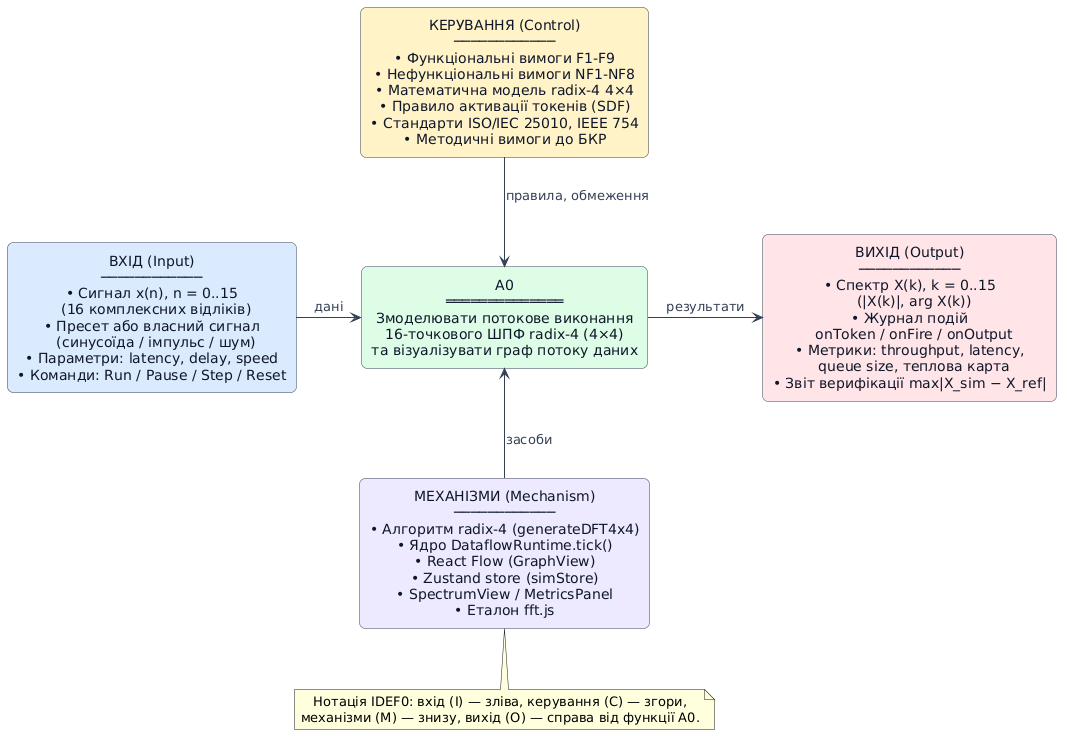
\includegraphics[width=6.49583in,height=4.51458in]{media/media/image1.png}

Рис. 1.1. Функцiональна IDEF0-схема задачi моделювання потокового
обчислювача ШПФ.

Результат роботи вважається досягнутим, якщо одночасно виконуються такі
вимірювані критерії:

\begin{itemize}
\item
  максимальне відхилення вихідного спектра симулятора від еталонного ДПФ
  за модулем не перевищує \(\varepsilon = 10^{- 9}\);
\item
  чотири вузли \passthrough{\lstinline!dft!}\passthrough{\lstinline!4!}
  першого ярусу виконуються паралельно, що підтверджується одночасними
  подіями \passthrough{\lstinline!onFire!} у журналі симуляції;
\item
  користувач може керувати швидкістю симуляції у діапазоні не менш ніж
  \(0.1 \times\) -- \(4 \times\) без втрати коректності;
\item
  час відгуку інтерфейсу на користувацькі дії (пуск, пауза, зміна
  швидкості) не перевищує 100 мс.
\end{itemize}

\protect\phantomsection\label{Xb0eb9a98447834cee65aa9c07744072b382be46}{}1.4.
Етичні, правові та регуляторні аспекти

Розроблюваний симулятор працює лише із синтетичними тестовими сигналами,
що формуються або вводяться користувачем у межах локального сеансу
роботи. Система не опрацьовує персональних, медичних, біометричних чи
фінансових даних, не передає інформацію на зовнішні сервери та не
використовує моделі штучного інтелекту для автоматизованого ухвалення
рішень. Тому вимоги GDPR і Закону України «Про захист персональних
даних» мають для цього проєкту обмежену прикладну релевантність, однак
базові принципи мінімізації даних, прозорості опрацювання та відсутності
прихованого збору інформації все одно дотримуються.

З регуляторного погляду для роботи суттєвими є насамперед вимоги до
якості програмного забезпечення, коректності числових обчислень та
оформлення результатів. У цьому контексті враховано положення
ISO/IEC\textasciitilde25010 щодо функціональної придатності,
продуктивності та зручності використання, стандарт
IEEE\textasciitilde754 щодо подання чисел з плаваючою крапкою, а також
ДСТУ\textasciitilde3008:2015 і
ДСТУ\textasciitilde ГОСТ\textasciitilde7.1:2006, які регламентують
оформлення пояснювальної записки та списку використаних джерел. Окремо
дотримується принцип академічної доброчесності: усі зовнішні джерела та
референтні реалізації належно процитовані, а отримані результати є
відтворюваними {[}24{]}{[}25{]}.

\protect\phantomsection\label{X124bb00a71ff7da6d40a6aa8e0ae644d11036d1}{}1.5.
Постановка задачі та формулювання вимог

Нехай задано комплекснозначну вхідну послідовність
\(\{ x_{n}\}_{n = 0}^{N - 1}\) довжиною \(N = 16\), подану у подвійній
точності формату IEEE 754 {[}24{]}. Потрібно розробити програмний
симулятор, який:

\begin{enumerate}
\def\labelenumi{\arabic{enumi})}
\item
  обчислює дискретне перетворення Фур'є за формулою (1.1):
\end{enumerate}

\[\begin{array}{r}
X_{k} = \sum_{n = 0}^{N - 1}x_{n}\, e^{- \frac{j2\pi nk}{N}},\quad k = 0,1,\ldots,N - 1,\ \#(1.1)
\end{array}\]

де \(X_{k}\) -- \(k\)-та комплексна спектральна компонента вихідної
послідовності;

\(x_{n}\) -- \(n\)-й комплексний відлік вхідної послідовності;

\(N = 16\) -- довжина перетворення;

за алгоритмом radix-4 з двовимірною \(4 \times 4\) декомпозицією,
реалізованим у моделі потоку даних;

\begin{enumerate}
\def\labelenumi{\arabic{enumi})}
\setcounter{enumi}{1}
\item
  подає процес обчислення у вигляді орієнтованого графа потоку даних
  \(G = (V,E)\), де \(V\) -- множина операцій, а \(E\) -- множина
  спрямованих зв\textquotesingle язків між ними;
\item
  виконує симуляцію графа з дотриманням правила активації (вузол
  спрацьовує тоді і лише тоді, коли на всіх його вхідних каналах є
  токени) та з урахуванням часових параметрів виконання операцій і
  передавання даних;
\item
  забезпечує інтерактивну візуалізацію процесу обчислення та подає
  кінцевий спектр \(\{ X_{k}\}\) у вигляді амплітудної діаграми.
\end{enumerate}

\textbf{Вхідні дані симулятора:}

\begin{itemize}
\item
  послідовність \(\{ x_{n}\}_{n = 0}^{15}\) -- 16 комплексних відліків
  сигналу, задається користувачем або генерується вбудованим джерелом
  (синусоїда, одиничний імпульс, білий шум);
\item
  параметри симуляції -- часові характеристики обробки, параметри
  передавання даних між операціями та множник швидкості відтворення;
\item
  команди керування -- пуск, пауза, покроковий режим, скидання стану.
\end{itemize}

\textbf{Вихідні дані симулятора:}

\begin{itemize}
\item
  спектр \(\{ X_{k}\}_{k = 0}^{15}\) -- 16 комплексних відліків, що
  візуалізуються як амплітуда \(|X_{k}|\) і фаза \(\arg X_{k}\);
\item
  журнал подій -- часові мітки надходження даних, активації операцій і
  формування результатів;
\item
  метрики роботи графа -- пропускна здатність (throughput), наскрізна
  затримка (latency), розмір черг (queue size), теплова карта активності
  вузлів;
\item
  звіт про верифікацію -- максимальне відхилення
  \(\max_{k}|X_{k}^{sim} - X_{k}^{ref}|\) відносно еталонного ДПФ.
\end{itemize}

Функціональні вимоги до симулятора зведено у табл. 1.3.

Таблиця 1.3

Функціональні вимоги до симулятора

\begin{longtable}[]{@{}
  >{\raggedright\arraybackslash}p{(\linewidth - 4\tabcolsep) * \real{0.0517}}
  >{\raggedright\arraybackslash}p{(\linewidth - 4\tabcolsep) * \real{0.2586}}
  >{\raggedright\arraybackslash}p{(\linewidth - 4\tabcolsep) * \real{0.6897}}@{}}
\caption[Функціональні вимоги до симулятора]{Функціональні вимоги до
симулятора}\tabularnewline
\toprule\noalign{}
\begin{minipage}[b]{\linewidth}\raggedright
\textbf{ID}
\end{minipage} & \begin{minipage}[b]{\linewidth}\raggedright
\textbf{Назва}
\end{minipage} & \begin{minipage}[b]{\linewidth}\raggedright
\textbf{Опис}
\end{minipage} \\
\midrule\noalign{}
\endfirsthead
\toprule\noalign{}
\begin{minipage}[b]{\linewidth}\raggedright
\textbf{ID}
\end{minipage} & \begin{minipage}[b]{\linewidth}\raggedright
\textbf{Назва}
\end{minipage} & \begin{minipage}[b]{\linewidth}\raggedright
\textbf{Опис}
\end{minipage} \\
\midrule\noalign{}
\endhead
\bottomrule\noalign{}
\endlastfoot
F1 & Побудова DFG & Автоматична генерація графа потоку даних для ШПФ
radix-4 \(4 \times 4\) при \(N = 16\) \\
F2 & Симуляція виконання & Крокування часу з доставкою токенів,
перевіркою правила активації та виконанням вузлів \\
F3 & Введення сигналу & Вибір типу вхідного сигналу (синусоїда, імпульс,
шум) та його параметрів \\
F4 & Керування симуляцією & Пуск, пауза, покроковий режим, скидання,
зміна множника швидкості \\
F5 & Візуалізація токенів & Анімоване переміщення токенів по дугах з
відображенням значень \\
F6 & Відображення метрик & Показ throughput, latency, queue size,
теплової карти активності \\
F7 & Спектральний вихід & Відображення амплітуди та фази \(\{ X_{k}\}\)
у вигляді гістограми \\
F8 & Верифікація результату & Порівняння з еталонним ДПФ і виведення
максимального відхилення \\
F9 & Налаштування параметрів & Редагування часових параметрів моделі без
перезавантаження сторінки \\
\end{longtable}

Нефункціональні вимоги регламентують якісні характеристики системи у
відповідності до ISO/IEC 25010 (табл. 1.4) {[}25{]}.

Таблиця 1.4

Нефункціональні вимоги до симулятора

\begin{longtable}[]{@{}
  >{\raggedright\arraybackslash}p{(\linewidth - 4\tabcolsep) * \real{0.0688}}
  >{\raggedright\arraybackslash}p{(\linewidth - 4\tabcolsep) * \real{0.2359}}
  >{\raggedright\arraybackslash}p{(\linewidth - 4\tabcolsep) * \real{0.6953}}@{}}
\caption[Нефункціональні вимоги до симулятора]{Нефункціональні вимоги до
симулятора}\tabularnewline
\toprule\noalign{}
\begin{minipage}[b]{\linewidth}\raggedright
\textbf{ID}
\end{minipage} & \begin{minipage}[b]{\linewidth}\raggedright
\textbf{Характеристика}
\end{minipage} & \begin{minipage}[b]{\linewidth}\raggedright
\textbf{Вимога}
\end{minipage} \\
\midrule\noalign{}
\endfirsthead
\toprule\noalign{}
\begin{minipage}[b]{\linewidth}\raggedright
\textbf{ID}
\end{minipage} & \begin{minipage}[b]{\linewidth}\raggedright
\textbf{Характеристика}
\end{minipage} & \begin{minipage}[b]{\linewidth}\raggedright
\textbf{Вимога}
\end{minipage} \\
\midrule\noalign{}
\endhead
\bottomrule\noalign{}
\endlastfoot
NF1 & Точність обчислень &
\(\max_{k}|X_{k}^{sim} - X_{k}^{ref}| \leq 10^{- 9}\) \\
NF2 & Час відгуку UI & Реакція на користувацьку дію \(\leq 100\) мс \\
NF3 & Частота кадрів & Стабільні 60 fps при швидкості симуляції
\(\leq 5 \times\) \\
NF4 & Портативність & Коректна робота у сучасних поширених
веб-браузерах \\
NF5 & Детермінованість & Однаковий вхід і параметри дають ідентичний
журнал подій \\
NF6 & Відкритий код & Розповсюдження під ліцензією MIT або Apache 2.0 \\
NF7 & Без встановлення & Робота у браузері без серверної частини та
БД \\
NF8 & Зручність & Основні операції доступні не глибше двох кліків від
головного екрану \\
\end{longtable}

У системі виділяються два актори -- \emph{Студент} (первинний
користувач, спостерігач) і \emph{Викладач} (вторинний користувач, може
налаштовувати сценарії демонстрації). Графічне подання прецедентів
наведено на рис. 1.2, а їхній деталізований перелік у табл. 1.5.

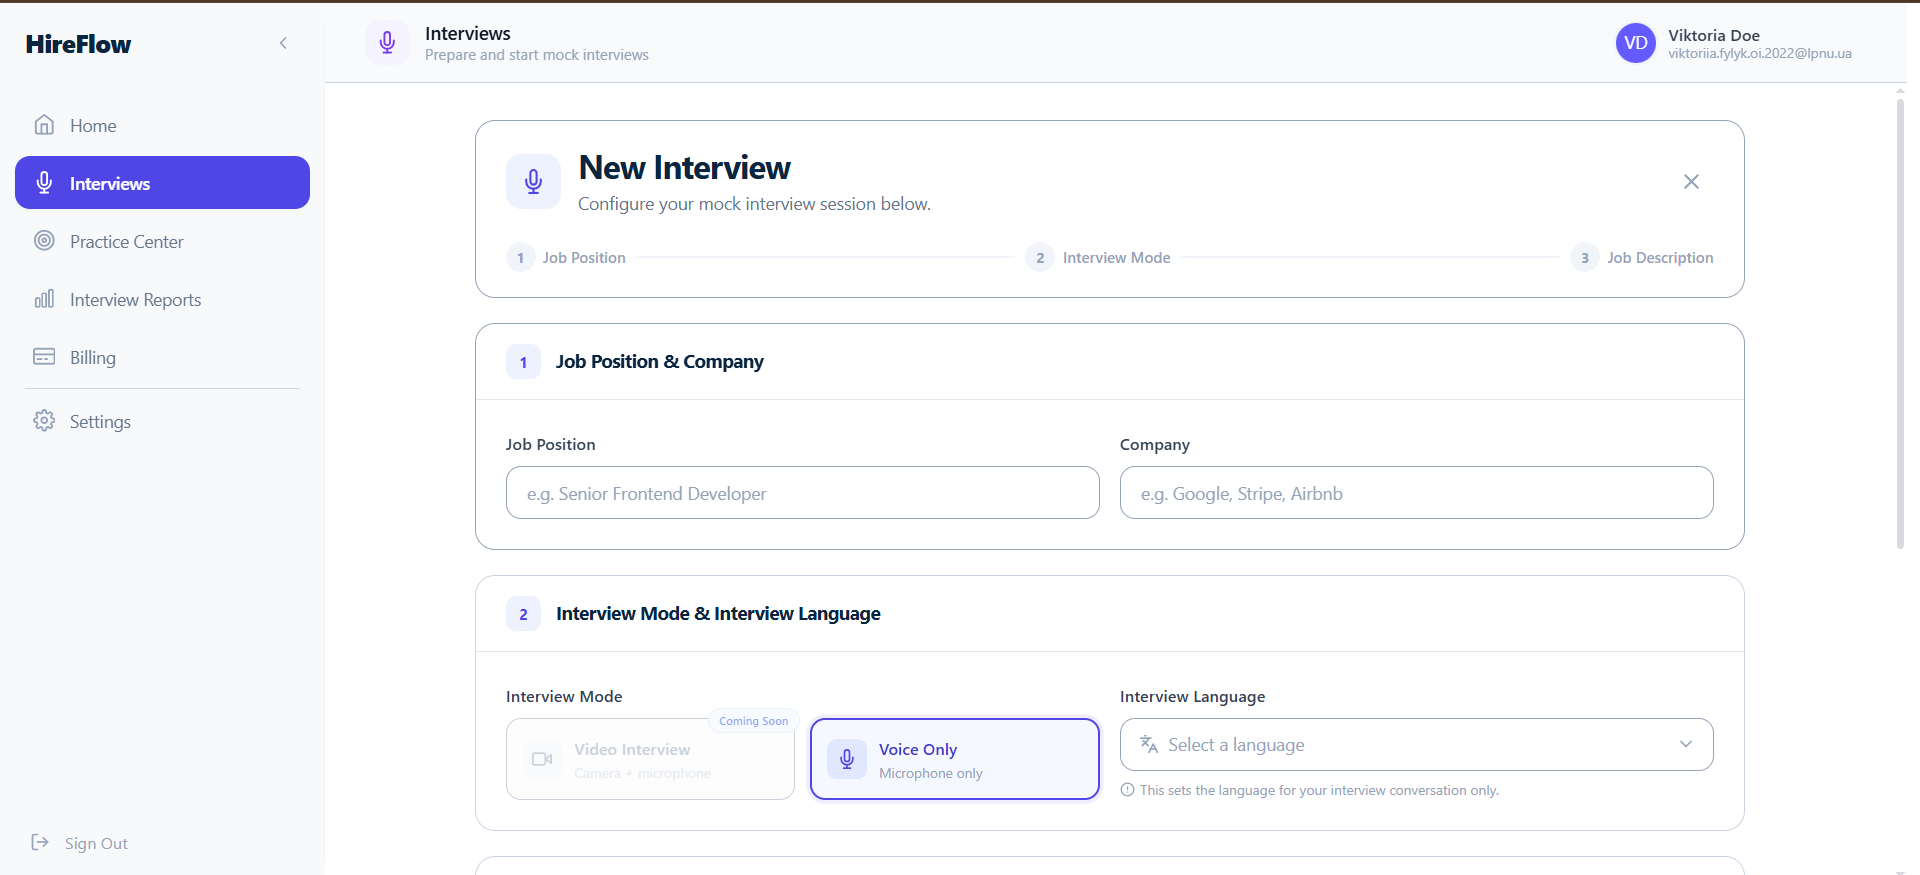
\includegraphics[width=6.49583in,height=4.64722in]{media/media/image2.png}

Рис. 1.2. Use Case-дiаграма симулятора потокового обчислювача ШПФ.

На дiаграмi показано, що UC3 мiстить (include) UC5, а UC7 розширює
(extend) UC3. Прецеденти UC1 i UC2 є взаємовиключними альтернативами
пiдготовки вхiдних даних. Посилання на табл

Таблиця 1.5

Перелік прецедентів (Use Cases) симулятора

\begin{longtable}[]{@{}
  >{\raggedright\arraybackslash}p{(\linewidth - 6\tabcolsep) * \real{0.0717}}
  >{\raggedright\arraybackslash}p{(\linewidth - 6\tabcolsep) * \real{0.2622}}
  >{\raggedright\arraybackslash}p{(\linewidth - 6\tabcolsep) * \real{0.1748}}
  >{\raggedright\arraybackslash}p{(\linewidth - 6\tabcolsep) * \real{0.4913}}@{}}
\caption[Перелік прецедентів (Use Cases) симулятора]{Перелік прецедентів
(Use Cases) симулятора}\tabularnewline
\toprule\noalign{}
\begin{minipage}[b]{\linewidth}\raggedright
\textbf{ID}
\end{minipage} & \begin{minipage}[b]{\linewidth}\raggedright
\textbf{Прецедент}
\end{minipage} & \begin{minipage}[b]{\linewidth}\raggedright
\textbf{Актор}
\end{minipage} & \begin{minipage}[b]{\linewidth}\raggedright
\textbf{Стислий опис}
\end{minipage} \\
\midrule\noalign{}
\endfirsthead
\toprule\noalign{}
\begin{minipage}[b]{\linewidth}\raggedright
\textbf{ID}
\end{minipage} & \begin{minipage}[b]{\linewidth}\raggedright
\textbf{Прецедент}
\end{minipage} & \begin{minipage}[b]{\linewidth}\raggedright
\textbf{Актор}
\end{minipage} & \begin{minipage}[b]{\linewidth}\raggedright
\textbf{Стислий опис}
\end{minipage} \\
\midrule\noalign{}
\endhead
\bottomrule\noalign{}
\endlastfoot
UC1 & Завантажити готовий сценарій & Студент, Викладач & Обрати один із
передустановлених входів (синусоїда, імпульс, шум) \\
UC2 & Задати власний вхідний сигнал & Студент & Ввести 16 комплексних
відліків вручну \\
UC3 & Запустити симуляцію & Студент & Ініціювати виконання DFG з пуску
до завершення \\
UC4 & Керувати темпом симуляції & Студент & Пауза, step-by-step, зміна
множника швидкості \\
UC5 & Спостерігати рух токенів & Студент & Переглядати анімацію токенів
по дугах у реальному часі \\
UC6 & Переглянути спектр результату & Студент & Побачити \(|X_{k}|\) і
\(\arg X_{k}\) у вигляді діаграми \\
UC7 & Порівняти з еталоном & Студент, Викладач & Виконати зіставлення з
референтним обчисленням і побачити похибку \\
UC8 & Змінити параметри затримок & Викладач & Налаштувати часові
характеристики вузлів і зв\textquotesingle язків графа \\
UC9 & Експортувати журнал подій & Викладач & Зберегти журнал подій у
файл для подальшого аналізу \\
\end{longtable}

\emph{Підпорядкування прецедентів:} UC3 містить (\emph{include}) UC5
(рух токенів автоматично супроводжує виконання); UC7 розширює
(\emph{extend}) UC3 та може бути викликаний після завершення симуляції;
UC1 і UC2 є взаємовиключними альтернативами підготовки вхідних даних.
Описана постановка задачі та перелік вимог утворюють технічне завдання,
яке далі конкретизується у розділі 2 через вибір методів і технологій
реалізації, проєктування архітектури та структур даних.

\protect\phantomsection\label{X075676d46328bd1f3c167fb2e80b0be216d8f0b}{}1.6.
Висновки до розділу 1

У першому розділі виконано аналіз предметної області, огляд сучасних
підходів, системний аналіз задачі, розгляд етичних та правових аспектів
і формалізовано постановку задачі.

Зафіксовано \emph{стан предметної області:} алгоритм ШПФ radix-4
\(4 \times 4\) для \(N = 16\) має достатньо розроблений математичний
апарат і формальні потокові моделі (DFG, SDF), однак у практичному
інструментарії ці рівні описані відокремлено. Виробничі бібліотеки
(FFTW, ARM CMSIS-DSP, NVIDIA CuFFT, SPIRAL, Intel IPP) оптимізовані
виключно для продуктивності та не надають засобів інтроспекції. Методи
візуального моделювання (UML, IDEF0, DFG/SDF, сигнальні графи)
залишаються переважно теоретичними та не реалізуються як інтерактивні
веб-симулятори з числовою верифікацією.

Виявлено \emph{прогалину:} жодне з розглянутих рішень не поєднує
одночасно достовірного обчислення ШПФ за формальною SDF-моделлю,
інтерактивної динамічної візуалізації руху токенів і веб-доступності без
комерційної ліцензії. Саме ця незаповнена ніша визначає предмет цієї
роботи.

Сформульовано \emph{задачу} розробки програмного симулятора потокового
обчислювача 16-точкового ШПФ з анімованим DFG, визначено вхідні та
вихідні дані, технічні, ресурсні й правові обмеження та критерії успіху.
Розроблено перелік із 9 функціональних (F1--F9) і 8 нефункціональних
(NF1--NF8) вимог, побудовано перелік із 9 прецедентів (UC1--UC9), що
охоплюють основні сценарії використання симулятора студентами та
викладачами. Ключові вимірювані критерії -- точність
\(\varepsilon \leq 10^{- 9}\), час відгуку \(\leq 100\) мс, стабільні 60
fps при швидкості до \(3 \times\) -- підлягають експериментальній
перевірці у розділі 4.

Розглянуто етичні та правові аспекти: робота не опрацьовує персональних
даних, базується на відкритих ліцензіях (MIT, Apache 2.0) і відповідає
стандартам ISO/IEC 25010, IEEE 754, ECMAScript 2020, ДСТУ 3008:2015 та
ДСТУ ГОСТ 7.1:2006. Математичне та алгоритмічне обґрунтування (виведення
формул radix-4 \(4 \times 4\), матричні факторизації, формалізація
DFG/SDF) виноситься до розділу 2, де воно подається у складі проєктного
обґрунтування обраних методів і архітектури системи.

\protect\phantomsection\label{_Toc230636411}{}РОЗДІЛ 2. ПРОЄКТУВАННЯ
ПРОГРАМНОГО РІШЕННЯ

\protect\phantomsection\label{X1a4d34ad0a12769944c99849904512a7f903224}{}2.1.
Вибір методів, технологій та засобів реалізації

У підрозд. 1.5 сформульовано технічне завдання: розробити веб-симулятор
потокового обчислювача 16-точкового ШПФ з інтерактивною візуалізацією
руху токенів, числовою верифікацією та відкритим доступом. У цьому
підрозділі обґрунтовується вибір архітектурних підходів, парадигм
реалізації та сімейств інструментів, що покривають ці вимоги. Конкретні
версії бібліотек та параметри середовища розробки наводяться у підрозд.
3.1.

Для визначення основного архітектурного підходу розглянуто три
альтернативи.

\textbf{Варіант А - настільний застосунок (Electron, Qt, JavaFX).}
Забезпечує повний доступ до ресурсів хост-системи та багатопоточність,
однак вимагає встановлення на кожну робочу станцію, окремих збірок під
різні ОС і суперечить вимозі NF7 (робота без встановлення).

\textbf{Варіант Б - клієнт-серверний веб-застосунок.} Передбачає
розміщення ядра симуляції на сервері, що вносить мережеву затримку,
несумісно з вимогою NF2 (час відгуку \(\leq 100\) мс), і потребує
підтримки серверної інфраструктури.

\textbf{Варіант В - повністю клієнтський SPA (Single-Page Application).}
\emph{Обрано як основу архітектури}: усі обчислення виконуються у
браузері, серверна частина відсутня, застосунок завантажується
одноразово як статичний пакет (HTML+JS+CSS) і надалі не потребує мережі.
Цей варіант одночасно задовольняє вимоги NF2, NF4 (портативність), NF5
(детермінованість) і NF7.

Посилання на

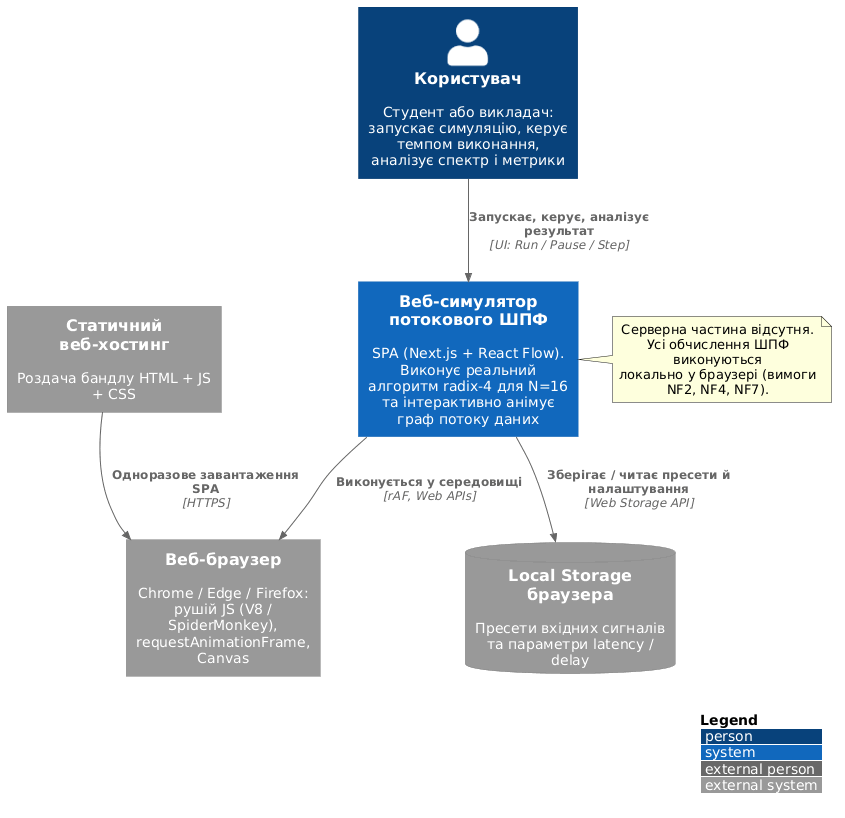
\includegraphics[width=4.952in,height=4.79265in]{media/media/image3.png}

Рис. 2.1. C4 Context-дiаграма веб-симулятора потокового обчислювача ШПФ.

Симулятор поєднує три принципово різні підсистеми: анімована графова
візуалізація DFG, числове ядро симуляції та панель керування і метрик.
Для їх ефективної координації обрано поєднання \emph{реактивного
рендерингу} та \emph{централізованого спостерігаваного сховища стану}.
Реактивний рендеринг (React-парадигма) природно відображає стан
симулятора на візуальні компоненти: зміна значення в одному полі сховища
автоматично ініціює перемалювання лише тих компонентів, що підписані на
це поле, що забезпечує стабільні 60 fps (NF3).

Централізоване сховище стану (pattern single source of truth) гарантує,
що всі панелі - GraphView, SpectrumView, Metrics -- бачать один і той
самий «знімок» стану у поточному кадрі. Альтернатива у вигляді прямого
маніпулювання DOM (jQuery-style) відкинута через лінійне зростання
складності, а Flux-підходи з ред'юсерами (Redux) -- надмірний обсяг
шаблонного коду.

Для реалізації інтерактивного графа потоку даних розглянуто рендеринг на
HTML-canvas (максимальна продуктивність, але ручна реалізація всіх
UI-взаємодій), SVG з ручним кодуванням (простіший налагодження, але
обмежена розширюваність) та спеціалізовану бібліотеку графової
візуалізації React\textasciitilde Flow. Обрано
React\textasciitilde Flow: бібліотека надає готові механізми
перетягування вузлів, зума, анімованих ребер і плаваючих підказок, а
формальна модель
\passthrough{\lstinline!Node!}/\passthrough{\lstinline!Edge!}, добре
відображається на абстракцію DFG.

У проєктуванні системи застосовано п'ять класичних шаблонів
проєктування:

\begin{itemize}
\item
  \emph{Observer (Publisher/Subscriber)} - забезпечує розсилку подій
  \passthrough{\lstinline!onToken!}, \passthrough{\lstinline!onFire!},
  \passthrough{\lstinline!onOutput!}: ядро симуляції є видавцем, а
  UI-компоненти - підписниками без прямих посилань на ядро;
\item
  \emph{State / Finite State Machine} - керує життєвим циклом симуляції:
  \passthrough{\lstinline!IDLE!} \(\rightarrow\)
  \passthrough{\lstinline!RUNNING!} \(\rightarrow\)
  \passthrough{\lstinline!PAUSED!} \(\rightarrow\)
  \passthrough{\lstinline!DONE!};
\item
  \emph{Strategy} -- забезпечує різні типи вузлів
  (\passthrough{\lstinline!source!},
  \passthrough{\lstinline!dft!}\passthrough{\lstinline!4!},
  \passthrough{\lstinline!twiddle!}, \passthrough{\lstinline!sink!}):
  поведінка вузла інкапсулюється у функції, обраній за полем
  \passthrough{\lstinline!NodeKind!};
\item
  \emph{Factory} -- реалізовано через функцію
  \passthrough{\lstinline!generateDFT!}\passthrough{\lstinline!4!}\passthrough{\lstinline!x!}\passthrough{\lstinline!4()!},
  що повертає готовий об'єкт \passthrough{\lstinline!Graph!} за
  параметрами \(N\) та \passthrough{\lstinline!latency!};
\item
  \emph{Facade} -- клас \passthrough{\lstinline!DataflowRuntime!}
  приховує внутрішню реалізацію черг і планувальника за єдиним публічним
  методом
  \passthrough{\lstinline!tick!}\passthrough{\lstinline!(!}\passthrough{\lstinline!dt!}\passthrough{\lstinline!,!}\passthrough{\lstinline! !}\passthrough{\lstinline!maxFires!}\passthrough{\lstinline!)!}.
\end{itemize}

Для дотримання NF1 (точність \(\varepsilon \leq 10^{- 9}\)) і NF5
(детермінованість) проєктом передбачено статичну типізацію вихідного
коду, що унеможливлює помилки передачі аргументів неправильного типу на
етапі компіляції. Комплексні числа подаються структурою\{ re, im \} у
подвійній точності IEEE 754, що забезпечує необхідний запас точності
{[}24{]}.

Підсумкова таблиця зв'язків між вимогами підрозд. 1.5 та обраними
архітектурними рішеннями наведена у табл. 2.1.

Таблиця 2.1

Зв'язок вимог і архітектурних рішень

\begin{longtable}[]{@{}
  >{\raggedright\arraybackslash}p{(\linewidth - 4\tabcolsep) * \real{0.2517}}
  >{\raggedright\arraybackslash}p{(\linewidth - 4\tabcolsep) * \real{0.3626}}
  >{\raggedright\arraybackslash}p{(\linewidth - 4\tabcolsep) * \real{0.3857}}@{}}
\caption[Зв'язок вимог і архітектурних рішень]{Зв'язок вимог і
архітектурних рішень}\tabularnewline
\toprule\noalign{}
\begin{minipage}[b]{\linewidth}\raggedright
\textbf{Вимога}
\end{minipage} & \begin{minipage}[b]{\linewidth}\raggedright
\textbf{Архітектурне рішення}
\end{minipage} & \begin{minipage}[b]{\linewidth}\raggedright
\textbf{Обґрунтування}
\end{minipage} \\
\midrule\noalign{}
\endfirsthead
\toprule\noalign{}
\begin{minipage}[b]{\linewidth}\raggedright
\textbf{Вимога}
\end{minipage} & \begin{minipage}[b]{\linewidth}\raggedright
\textbf{Архітектурне рішення}
\end{minipage} & \begin{minipage}[b]{\linewidth}\raggedright
\textbf{Обґрунтування}
\end{minipage} \\
\midrule\noalign{}
\endhead
\bottomrule\noalign{}
\endlastfoot
NF1 (точність) & Статична типізація + IEEE 754 double & Виключення
помилок типів, \(\varepsilon_{mach} \approx 2.22 \cdot 10^{- 16}\) \\
NF2 (відгук \(\leq 100\) мс) & Клієнтський SPA без серверних викликів &
Відсутність мережевої затримки \\
NF3 (60 fps) & Реактивний рендеринг з підпискою на окремі поля &
Перемальовування лише змінених компонентів \\
NF4 (портативність) & Стандарт ES2020, Web APIs & Робота у
Chrome/Firefox/Edge без polyfill \\
NF5 (детермінованість) & Логічний час + статичний граф & Ідентичні входи
\(\Rightarrow\) ідентичний журнал \\
NF6 (MIT/Apache) & Вибір лише OSS-бібліотек & React, React Flow,
Zustand, TypeScript \\
NF7 (без встановлення) & SPA у статичному хостингу & Одноразове
завантаження бандлу \\
NF8 (зручність) & React Flow + панелі Controls/Metrics & Двокліковий
доступ до базових операцій \\
\end{longtable}

\protect\phantomsection\label{Xe17a367fa0386aee11bbb4389e0e3ba247fd242}{}2.2.
Математичне та алгоритмічне забезпечення

У цьому підрозділі подано математичний апарат 16-точкового ШПФ з основою
4, що становить інтелектуальне ядро симулятора, та формалізацію
обчислень у парадигмі потоку даних.

Дискретне перетворення Фур'є (ДПФ) скінченної комплекснозначної
послідовності \(\{ x_{n}\}_{n = 0}^{N - 1}\) визначається за формулою
(2.1) (Nussbaumer 1982; Процько et al. 2025):

\[\begin{array}{r}
X_{k} = \sum_{n = 0}^{N - 1}x_{n}\, e^{- \frac{j2\pi nk}{N}} = \sum_{n = 0}^{N - 1}x_{n}\, W_{N}^{nk},\quad k = 0,1,\ldots,N - 1,\ \#(2.1)
\end{array}\]

де \(X_{k}\) -- \(k\)-та комплексна спектральна компонента;

\(x_{n}\) -- \(n\)-й комплексний відлік вхідної послідовності;

\(N = 16\) -- довжина перетворення;

\(W_{N} = e^{- j2\pi/N}\) -- поворотний множник (twiddle factor). Пряме
обчислення~потребує \(N^{2}\) комплексних множень, тобто має складність
\(O(N^{2})\), що недостатньо для задач реального часу. Клас швидких
алгоритмів (ШПФ) знижує складність до \(O(N\log_{2}N)\) за рахунок
факторизації \(N = N_{1} \cdot N_{2}\). Для \(N = 16\) природним вибором
є алгоритм з основою~4 (radix-4), де \(N_{1} = N_{2} = 4\) (Cooley and
Tukey 1965).

Для двовимірної \(4 \times 4\) декомпозиції часовий і частотний індекси
подаються згідно з (2.2){[}22{]}:

\[\begin{array}{r}
n = 4s + r,\quad k = 4k_{2} + k_{1},\quad r,s,k_{1},k_{2} \in \left\{ 0,1,2,3 \right\},\ \#(2.2)
\end{array}\]

де \(n\) -- лінійний індекс вхідного відліку, \(n = 0,\ldots,15\);

\(k\) -- лінійний індекс спектрального відліку, \(k = 0,\ldots,15\);

\(r,s\) -- індекси рядка і стовпця вхідної матриці;

\(k_{1},k_{2}\) -- індекси стовпця і рядка вихідної матриці.

Вхідна послідовність \(\{ x(n)\}_{n = 0}^{15}\) вкладається у матрицю
\(\mathbf{A}\) розміром \(4 \times 4\) за формулою~(2.3):

\[\begin{array}{r}
A\lbrack r\rbrack\lbrack s\rbrack = x(4s + r),\quad r,s \in \left\{ 0,1,2,3 \right\},\ \#(2.3)
\end{array}\]

де \(A\lbrack r\rbrack\lbrack s\rbrack\) -- елемент вхідної матриці у
рядку \(r\) і стовпці \(s\);

\(x(n)\) -- значення вхідної послідовності з лінійним індексом
\(n = 4s + r\).

Підстановка у формулу ДПФ із використанням тотожності
\(W_{16}^{4 \cdot ( \cdot )} = W_{4}^{( \cdot )}\) дає тристадійну
схему, описану виразом (2.4) та показану на рисунку (\textbf{рис. Г.1}.)
(Burrus and Parks 1985; Nussbaumer 1982):

\[\begin{array}{r}
X(4k_{2} + k_{1}) = \sum_{r = 0}^{3}W_{16}^{rk_{1}}\underset{G_{r}(k_{1})}{\underbrace{\left( \sum_{s = 0}^{3}A\lbrack r\rbrack\lbrack s\rbrack\, W_{4}^{sk_{1}} \right)}}W_{4}^{rk_{2}},\#(2.4)
\end{array}\]

де \(X(4k_{2} + k_{1})\) -- спектральний відлік з індексом
\(k = 4k_{2} + k_{1}\);

\(G_{r}(k_{1})\) -- результат рядкового 4-точкового ДПФ (стадія~1);

\(W_{16}^{rk_{1}}\) -- поворотний множник стадії~2;

\(W_{4}^{rk_{2}}\) -- ядро стовпцевого 4-точкового ДПФ (стадія~3).

\textbf{Стадія 1 -- рядкові 4-точкові ДПФ.} Для кожного
\(r \in \{ 0,1,2,3\}\) обчислюється 4-точкове ДПФ рядка за формулою
(2.5):

\[\begin{array}{r}
G_{r}\left( k_{1} \right) = \sum_{s = 0}^{3}A\lbrack r\rbrack\lbrack s\rbrack\, W_{4}^{sk_{1}},\quad k_{1} \in \left\{ 0,1,2,3 \right\},\ \#(2.5)
\end{array}\]

де \(G_{r}(k_{1})\) -- \(k_{1}\)-та компонента 4-точкового ДПФ \(r\)-го
рядка матриці~\(\mathbf{A}\);

\(A\lbrack r\rbrack\lbrack s\rbrack\) -- елемент рядка \(r\), визначений
формулою~(2.3);

\(W_{4} = e^{- j2\pi/4} = - j\) -- поворотний множник 4-точкового ядра.

Чотири ці перетворення є взаємно незалежними та виконуються паралельно.

\textbf{Стадія 2 -- поворотні множники.} Результати стадії 1 множаться
на матрицю поворотних множників згідно з (2.6):

\[\begin{array}{r}
H_{r}\left( k_{1} \right) = W_{16}^{r \cdot k_{1}} \cdot G_{r}\left( k_{1} \right),\quad r,k_{1} \in \left\{ 0,1,2,3 \right\},\ \#(2.6)
\end{array}\]

де \(H_{r}(k_{1})\) -- проміжне значення після множення на поворотний
множник;

\(W_{16}^{r \cdot k_{1}} = e^{- j2\pi rk_{1}/16}\) -- поворотний множник
\(16\)-точкового ШПФ;

\(G_{r}(k_{1})\) -- вихід стадії~1 згідно з~(2.5).

При \(r = 0\) або \(k_{1} = 0\) маємо \(W_{16}^{0} = 1\), тому 7 з 16
множень є тривіальними. Числові значення 9 нетривіальних множників
наведено у табл. 2.2.

Таблиця 2.2

Поворотні множники
\(\mathbf{W}_{\mathbf{16}}^{\mathbf{r}\mathbf{\cdot}\mathbf{k}_{\mathbf{1}}}\)
(округлено до 3 знаків)

\begin{longtable}[]{@{}
  >{\raggedright\arraybackslash}p{(\linewidth - 8\tabcolsep) * \real{0.0871}}
  >{\raggedright\arraybackslash}p{(\linewidth - 8\tabcolsep) * \real{0.0375}}
  >{\raggedright\arraybackslash}p{(\linewidth - 8\tabcolsep) * \real{0.1883}}
  >{\raggedright\arraybackslash}p{(\linewidth - 8\tabcolsep) * \real{0.2076}}
  >{\raggedright\arraybackslash}p{(\linewidth - 8\tabcolsep) * \real{0.2076}}@{}}
\caption[Поворотні множники W\_\{16\}\^{}\{r \textbackslash cdot
k\_\{1\}\} (округлено до 3 знаків)]{Поворотні множники W\_\{16\}\^{}\{r
\textbackslash cdot k\_\{1\}\} (округлено до 3 знаків)}\tabularnewline
\toprule\noalign{}
\begin{minipage}[b]{\linewidth}\centering
\[r \smallsetminus k_{1}\]
\end{minipage} & \begin{minipage}[b]{\linewidth}\raggedright
0
\end{minipage} & \begin{minipage}[b]{\linewidth}\raggedright
1
\end{minipage} & \begin{minipage}[b]{\linewidth}\raggedright
2
\end{minipage} & \begin{minipage}[b]{\linewidth}\raggedright
3
\end{minipage} \\
\midrule\noalign{}
\endfirsthead
\toprule\noalign{}
\begin{minipage}[b]{\linewidth}\centering
\[r \smallsetminus k_{1}\]
\end{minipage} & \begin{minipage}[b]{\linewidth}\raggedright
0
\end{minipage} & \begin{minipage}[b]{\linewidth}\raggedright
1
\end{minipage} & \begin{minipage}[b]{\linewidth}\raggedright
2
\end{minipage} & \begin{minipage}[b]{\linewidth}\raggedright
3
\end{minipage} \\
\midrule\noalign{}
\endhead
\bottomrule\noalign{}
\endlastfoot
& \(1\) & \(1\) & \(1\) & \(1\) \\
& \(1\) & \(0,924 - 0,383j\) & \(0,707 - 0,707j\) &
\(0,383 - 0,924j\) \\
& \(1\) & \(0,707 - 0,707j\) & \(- j\) & \(- 0,707 - 0,707j\) \\
& \(1\) & \(0,383 - 0,924j\) & \(- 0,707 - 0,707j\) &
\(- 0,924 + 0,383j\) \\
\end{longtable}

\textbf{Стадія 3 -- стовпцеві 4-точкові ДПФ.} Для кожного \(k_{1}\)
обчислюється 4-точкове ДПФ стовпця матриці \(\mathbf{H}\) за формулою
(2.7):

\[\begin{array}{r}
X\left( 4k_{2} + k_{1} \right) = \sum_{r = 0}^{3}H_{r}\left( k_{1} \right)\, W_{4}^{rk_{2}},\quad k_{2} \in \left\{ 0,1,2,3 \right\},\ \#(2.7)
\end{array}\]

де \(X(4k_{2} + k_{1})\) -- вихідний спектральний відлік з індексом
\(k = 4k_{2} + k_{1}\);

\(H_{r}(k_{1})\) -- проміжне значення після стадії~2 згідно з~(2.6);

\(W_{4}^{rk_{2}}\) -- поворотний множник 4-точкового ядра.

Чотири стовпцевих перетворення також є взаємно незалежними.

Ядром обох стадій є 4-точкове ДПФ, що завдяки властивостям
\(W_{4} \in \{ 1, - j, - 1,j\}\) реалізується без нетривіальних множень.
Для входів \(v_{0},v_{1},v_{2},v_{3}\mathbb{\in C}\) вводяться проміжні
суми і різниці (2.8):

\[\begin{array}{r}
E_{0} = v_{0} + v_{2},\quad E_{1} = v_{0} - v_{2},\ \#(2.8)
\end{array}\]

\[O_{0} = v_{1} + v_{3},\quad O_{1} = v_{1} - v_{3},\]

де \(v_{0},v_{1},v_{2},v_{3}\) -- комплексні входи 4-точкового ядра;

\(E_{0},E_{1}\) -- проміжні суми і різниці парних входів;

\(O_{0},O_{1}\) -- проміжні суми і різниці непарних входів.

Після цього обчислюються вихідні відліки 4-точкового ДПФ~(2.9):

\[\begin{array}{r}
\begin{aligned}
V_{0} & = E_{0} + O_{0}, & V_{2} & = E_{0} - O_{0}, \\
V_{1} & = E_{1} - j \cdot O_{1}, & V_{3} & = E_{1} + j \cdot O_{1}.
\end{aligned}\ \#(2.9)
\end{array}\]

де \(V_{0},V_{1},V_{2},V_{3}\) -- вихідні комплексні значення
4-точкового ДПФ;

\(E_{0},E_{1},O_{0},O_{1}\) -- проміжні значення згідно з~(2.8);

\(j\) -- уявна одиниця.

Множення на \(j\) зводиться до перестановки дійсної та уявної частин зі
зміною знаку (\(j \cdot (a + bj) = - b + aj\)) і не потребує операції
множення у традиційному сенсі. Таким чином, одне 4-точкове ДПФ потребує
\textbf{8 комплексних додавань і 0 нетривіальних множень} (Nussbaumer
1982).

Загальна обчислювальна вартість алгоритму для \(N = 16\):

\begin{itemize}
\item
  \textbf{Стадія 1:} \(4 \cdot 8 = 32\) комплексних додавань;
\item
  \textbf{Стадія 2:} \(9\) нетривіальних комплексних множень (\(36\)
  дійсних) і \(16\) комплексних додавань;
\item
  \textbf{Стадія 3:} \(4 \cdot 8 = 32\) комплексних додавань.
\end{itemize}

Разом: \textbf{9 нетривіальних комплексних множень} і \textbf{80
комплексних додавань}, порівняно з \(N^{2} = 256\) множень прямого ДПФ -
прискорення у \(\approx 28\) разів за кількістю множень (Nussbaumer
1982; Burrus and Parks 1985).

Алгоритм подається у вигляді орієнтованого ациклічного графа потоку
даних (DFG) \(G = (V,E)\) (Dennis 1974; Lee and Hurson 1994), де:

\begin{itemize}
\item
  \(V\) -- множина вузлів чотирьох типів
  (\passthrough{\lstinline!source!},
  \passthrough{\lstinline!dft!}\passthrough{\lstinline!4!},
  \passthrough{\lstinline!twiddle!}, \passthrough{\lstinline!sink!});
\item
  \(E \subseteq V \times V\) -- множина спрямованих дуг, що є
  FIFO-чергами токенів.
\end{itemize}

\textbf{Правило активації.} Вузол \(v \in V\) є готовим до виконання
тоді і лише тоді, коли на кожному з його вхідних каналів присутній
щонайменше один токен. При активації він поглинає вхідні токени, виконує
обчислення та породжує вихідні токени.

\textbf{Часова модель.} Вузол має затримку виконання
\passthrough{\lstinline!latency!}, а дуга -- затримку доставки
\passthrough{\lstinline!delay!}. Токен, породжений у момент \(t\), стає
готовим у момент \(t + \text{delay}\). Логічний час \(\tau\) симулятора
інкрементується дискретно на кроці \(d\tau\), що регулюється множником
швидкості.

Планувальник (ядро \passthrough{\lstinline!DataflowRuntime!}) на кожному
кроці симуляції виконує доставку токенів із FIFO-черг і запуск готових
вузлів. Узагальнений псевдокод наведено нижче

{\def\LTcaptype{none} % do not increment counter
\begin{longtable}[]{@{}
  >{\raggedright\arraybackslash}p{(\linewidth - 0\tabcolsep) * \real{0.5353}}@{}}
\toprule\noalign{}
\endhead
\bottomrule\noalign{}
\endlastfoot
\begin{minipage}[t]{\linewidth}\raggedright
\passthrough{\lstinline!procedure!}\passthrough{\lstinline! !}\passthrough{\lstinline!TICK(dt,!}\passthrough{\lstinline! !}\passthrough{\lstinline!maxFires!}\passthrough{\lstinline!)!}\strut \\
\passthrough{\lstinline!    !}\passthrough{\lstinline!tau!}\passthrough{\lstinline! !}\passthrough{\lstinline!<-!}\passthrough{\lstinline! !}\passthrough{\lstinline!tau!}\passthrough{\lstinline! !}\passthrough{\lstinline!+!}\passthrough{\lstinline! !}\passthrough{\lstinline!dt!}\strut \\
\passthrough{\lstinline!    !}\passthrough{\lstinline!for!}\passthrough{\lstinline! !}\passthrough{\lstinline!each!}\passthrough{\lstinline! !}\passthrough{\lstinline!edge!}\passthrough{\lstinline! !}\passthrough{\lstinline!e!}\passthrough{\lstinline! !}\passthrough{\lstinline!in!}\passthrough{\lstinline! !}\passthrough{\lstinline!E!}\strut \\
\passthrough{\lstinline!        !}\passthrough{\lstinline!while!}\passthrough{\lstinline! !}\passthrough{\lstinline!e.queue.head.t!}\passthrough{\lstinline! !}\passthrough{\lstinline!+!}\passthrough{\lstinline! !}\passthrough{\lstinline!e.delay!}\passthrough{\lstinline! !}\passthrough{\lstinline!<=!}\passthrough{\lstinline! !}\passthrough{\lstinline!tau!}\strut \\
\passthrough{\lstinline!            !}\passthrough{\lstinline!token!}\passthrough{\lstinline! !}\passthrough{\lstinline!<-!}\passthrough{\lstinline! !}\passthrough{\lstinline!e.queue.pop!}\passthrough{\lstinline!()!}\strut \\
\passthrough{\lstinline!            !}\passthrough{\lstinline!v!}\passthrough{\lstinline! !}\passthrough{\lstinline!<-!}\passthrough{\lstinline! !}\passthrough{\lstinline!target(e);!}\passthrough{\lstinline! !}\passthrough{\lstinline!port!}\passthrough{\lstinline! !}\passthrough{\lstinline!<-!}\passthrough{\lstinline! !}\passthrough{\lstinline!targetPort!}\passthrough{\lstinline!(e)!}\strut \\
\passthrough{\lstinline!            !}\passthrough{\lstinline!v.inputs!}\passthrough{\lstinline![port]!}\passthrough{\lstinline! !}\passthrough{\lstinline!<-!}\passthrough{\lstinline! !}\passthrough{\lstinline!token!}\strut \\
\passthrough{\lstinline!    !}\passthrough{\lstinline!fires!}\passthrough{\lstinline! !}\passthrough{\lstinline!<-!}\passthrough{\lstinline! !}\passthrough{\lstinline!0!}\strut \\
\passthrough{\lstinline!    !}\passthrough{\lstinline!for!}\passthrough{\lstinline! !}\passthrough{\lstinline!each!}\passthrough{\lstinline! !}\passthrough{\lstinline!node!}\passthrough{\lstinline! !}\passthrough{\lstinline!v!}\passthrough{\lstinline! !}\passthrough{\lstinline!in!}\passthrough{\lstinline! !}\passthrough{\lstinline!V!}\passthrough{\lstinline!  !}\passthrough{\lstinline!order!}\passthrough{\lstinline! !}\passthrough{\lstinline!by!}\passthrough{\lstinline! !}\passthrough{\lstinline!id!}\strut \\
\passthrough{\lstinline!        !}\passthrough{\lstinline!if!}\passthrough{\lstinline! !}\passthrough{\lstinline!v!}\passthrough{\lstinline! !}\passthrough{\lstinline!is!}\passthrough{\lstinline! !}\passthrough{\lstinline!ready!}\passthrough{\lstinline! !}\passthrough{\lstinline!and!}\passthrough{\lstinline! !}\passthrough{\lstinline!not!}\passthrough{\lstinline! !}\passthrough{\lstinline!busy!}\passthrough{\lstinline! !}\passthrough{\lstinline!and!}\passthrough{\lstinline! !}\passthrough{\lstinline!fires!}\passthrough{\lstinline! !}\passthrough{\lstinline!<!}\passthrough{\lstinline! !}\passthrough{\lstinline!maxFires!}\strut \\
\passthrough{\lstinline!            !}\passthrough{\lstinline!emit!}\passthrough{\lstinline! !}\passthrough{\lstinline!onFire!}\passthrough{\lstinline!(v,!}\passthrough{\lstinline! !}\passthrough{\lstinline!tau)!}\strut \\
\passthrough{\lstinline!            !}\passthrough{\lstinline!v.busy!}\passthrough{\lstinline! !}\passthrough{\lstinline!<-!}\passthrough{\lstinline! !}\passthrough{\lstinline!tau!}\passthrough{\lstinline! !}\passthrough{\lstinline!+!}\passthrough{\lstinline! !}\passthrough{\lstinline!v.latency!}\strut \\
\passthrough{\lstinline!            !}\passthrough{\lstinline!outs!}\passthrough{\lstinline! !}\passthrough{\lstinline!<-!}\passthrough{\lstinline! !}\passthrough{\lstinline!compute(!}\passthrough{\lstinline!v.kind!}\passthrough{\lstinline!,!}\passthrough{\lstinline! !}\passthrough{\lstinline!v.inputs!}\passthrough{\lstinline!)!}\strut \\
\passthrough{\lstinline!            !}\passthrough{\lstinline!schedule!}\passthrough{\lstinline! !}\passthrough{\lstinline!outs!}\passthrough{\lstinline! !}\passthrough{\lstinline!on!}\passthrough{\lstinline! !}\passthrough{\lstinline!outgoing!}\passthrough{\lstinline! !}\passthrough{\lstinline!edges!}\passthrough{\lstinline! !}\passthrough{\lstinline!at!}\passthrough{\lstinline! !}\passthrough{\lstinline!time!}\passthrough{\lstinline! !}\passthrough{\lstinline!v.busy!}\strut \\
\passthrough{\lstinline!            !}\passthrough{\lstinline!fires!}\passthrough{\lstinline! !}\passthrough{\lstinline!<-!}\passthrough{\lstinline! !}\passthrough{\lstinline!fires!}\passthrough{\lstinline! !}\passthrough{\lstinline!+!}\passthrough{\lstinline! !}\passthrough{\lstinline!1!}\strut \\
\passthrough{\lstinline!    !}\passthrough{\lstinline!for!}\passthrough{\lstinline! !}\passthrough{\lstinline!each!}\passthrough{\lstinline! !}\passthrough{\lstinline!node!}\passthrough{\lstinline! !}\passthrough{\lstinline!v!}\passthrough{\lstinline! !}\passthrough{\lstinline!in!}\passthrough{\lstinline! !}\passthrough{\lstinline!V!}\strut \\
\passthrough{\lstinline!        !}\passthrough{\lstinline!if!}\passthrough{\lstinline! !}\passthrough{\lstinline!v.busy!}\passthrough{\lstinline! !}\passthrough{\lstinline!<=!}\passthrough{\lstinline! !}\passthrough{\lstinline!tau!}\passthrough{\lstinline! !}\passthrough{\lstinline!then!}\passthrough{\lstinline! !}\passthrough{\lstinline!v.busy!}\passthrough{\lstinline! !}\passthrough{\lstinline!<-!}\passthrough{\lstinline! !}\passthrough{\lstinline!0!}\strut
\end{minipage} \\
\end{longtable}
}

Рис. Псевдокод однієї ітерації ядра симуляції
\passthrough{\lstinline!DataflowRuntime!}\passthrough{\lstinline!.!}\passthrough{\lstinline!tick!}\passthrough{\lstinline!()!}.
Джерело: розроблено автором.

Ця процедура забезпечує детермінованість (NF5): при фіксованому порядку
обходу вузлів результат симуляції не залежить від реального часу
виконання у браузері.

\protect\phantomsection\label{X8971522f2fc6036ff7f6d6d494a0986f56fee46}{}2.3.
Загальна архітектура системи

Архітектура симулятора описується на двох рівнях моделі C4 (Brown 2018)
-- Context і Container, -- доповнених діаграмою потоків даних.

На контекстному рівні система представляється як «чорна скринька», що
взаємодіє з одним актором -- \emph{користувачем} (студент або викладач),
та з двома зовнішніми сутностями: \emph{браузером} (runtime-середовище)
і \emph{локальним сховищем браузера} (для збереження пресетів вхідних
сигналів). Застосунок завантажується одноразово зі статичного
веб-хостингу та надалі працює автономно.

На рівні контейнерів симулятор декомпозується на чотири логічні
підсистеми, що виконуються у межах одного процесу браузера:

\begin{enumerate}
\def\labelenumi{\arabic{enumi})}
\item
  \textbf{Simulation Core} - реалізує псевдокод підрозд. 2.2, зберігає
  стан графа та черг;
\item
  \textbf{Graph Generator} -- модуль побудови DFG для заданого \(N\) та
  параметрів затримок;
\item
  \textbf{State Store} -- централізоване сховище стану, до якого
  підписуються всі UI-компоненти;
\item
  \textbf{UI Layer} -- набір React-компонентів:
  \passthrough{\lstinline!GraphView!} (полотно React Flow),
  \passthrough{\lstinline!SpectrumView!} (діаграма \(|X(k)|\)),
  \passthrough{\lstinline!Metrics!} (пропускна здатність, затримка,
  черги), \passthrough{\lstinline!Controls!} (пуск/пауза/швидкість).
\end{enumerate}

UI Layer читає стан зі State Store та викликає команди; State Store
делегує обробку до Simulation Core; Simulation Core публікує події
(\passthrough{\lstinline!onToken!}, \passthrough{\lstinline!onFire!},
\passthrough{\lstinline!onOutput!}), на які State Store оновлює
відповідні поля; Graph Generator викликається один раз при ініціалізації
та при кожній зміні параметрів.

Контейнерну декомпозицiю системи з основними потоками керування та даних
подано на рис. 2.3.


\includegraphics[width=6.4375in,height=3.8519in]{media/media/image4.png}

Рис. 2.3. C4 Container-дiаграма архiтектури веб-симулятора.

Детальна структура DFG для \(N = 16\) складається з \textbf{56 вузлів} і
\textbf{64 дуг}, як показано на рисунку (рис. Г.2.), розподілених за
п'ятьма ярусами:

\begin{enumerate}
\def\labelenumi{\arabic{enumi})}
\item
  16 вузлів \passthrough{\lstinline!source!}
  (src\(_{0}\ldots\)src\(_{15}\)) -- генерують токени вхідних відліків
  \(x(n)\);
\item
  4 вузли \passthrough{\lstinline!dft!}\passthrough{\lstinline!4!}
  (row-0 \ldots row-3) -- виконують рядкові ДПФ (стадія 1);
\item
  16 вузлів \passthrough{\lstinline!twiddle!} (tw-\(r\)-\(k_{1}\); у
  вихідному коді --
  \passthrough{\lstinline!tw!}\passthrough{\lstinline!-!}\(n_{1}\)\passthrough{\lstinline!-!}\(k_{2}\),
  де \(n_{1} \equiv r\), \(k_{2} \equiv k_{1}\), а степінь множника
  \(n_{1}k_{2} \equiv rk_{1}\)) -- множать на поворотні множники (стадія
  2);
\item
  4 вузли \passthrough{\lstinline!dft!}\passthrough{\lstinline!4!}
  (col-0 \ldots col-3) -- виконують стовпцеві ДПФ (стадія 3);
\item
  16 вузлів \passthrough{\lstinline!sink!}
  (snk\(_{0}\ldots\)snk\(_{15}\)) -- збирають спектральні відліки
  \(X(k)\).
\end{enumerate}

Характеристики вузлів і дуг зведено у табл. 2.3 -- 2.4.

Таблиця 2.3

Типи вузлів DFG та їхні характеристики

\begin{longtable}[]{@{}
  >{\raggedright\arraybackslash}p{(\linewidth - 10\tabcolsep) * \real{0.1261}}
  >{\raggedright\arraybackslash}p{(\linewidth - 10\tabcolsep) * \real{0.0793}}
  >{\raggedright\arraybackslash}p{(\linewidth - 10\tabcolsep) * \real{0.1295}}
  >{\raggedright\arraybackslash}p{(\linewidth - 10\tabcolsep) * \real{0.1412}}
  >{\raggedright\arraybackslash}p{(\linewidth - 10\tabcolsep) * \real{0.1254}}
  >{\raggedright\arraybackslash}p{(\linewidth - 10\tabcolsep) * \real{0.3985}}@{}}
\caption[Типи вузлів DFG та їхні характеристики]{Типи вузлів DFG та їхні
характеристики}\tabularnewline
\toprule\noalign{}
\begin{minipage}[b]{\linewidth}\raggedright
Тип вузла
\end{minipage} & \begin{minipage}[b]{\linewidth}\raggedright
К-сть
\end{minipage} & \begin{minipage}[b]{\linewidth}\raggedright
Вх. портів
\end{minipage} & \begin{minipage}[b]{\linewidth}\raggedright
Вих. портів
\end{minipage} & \begin{minipage}[b]{\linewidth}\raggedright
Затримка
\end{minipage} & \begin{minipage}[b]{\linewidth}\raggedright
Функція
\end{minipage} \\
\midrule\noalign{}
\endfirsthead
\toprule\noalign{}
\begin{minipage}[b]{\linewidth}\raggedright
Тип вузла
\end{minipage} & \begin{minipage}[b]{\linewidth}\raggedright
К-сть
\end{minipage} & \begin{minipage}[b]{\linewidth}\raggedright
Вх. портів
\end{minipage} & \begin{minipage}[b]{\linewidth}\raggedright
Вих. портів
\end{minipage} & \begin{minipage}[b]{\linewidth}\raggedright
Затримка
\end{minipage} & \begin{minipage}[b]{\linewidth}\raggedright
Функція
\end{minipage} \\
\midrule\noalign{}
\endhead
\bottomrule\noalign{}
\endlastfoot
\passthrough{\lstinline!source!} & & & & -- & Генерація \(x(n)\) \\
\passthrough{\lstinline!dft4!} & & & & & -точкове ДПФ (метелик з
підрозд. 2.2) \\
\passthrough{\lstinline!twiddle!} & & & & & Множення на
\(W_{16}^{rk_{1}}\) \\
\passthrough{\lstinline!sink!} & & & & -- & Збір \(X(k)\) \\
& & & & & \\
\end{longtable}

Таблиця 2.4

Типи дуг DFG

\begin{longtable}[]{@{}
  >{\raggedright\arraybackslash}p{(\linewidth - 6\tabcolsep) * \real{0.1277}}
  >{\raggedright\arraybackslash}p{(\linewidth - 6\tabcolsep) * \real{0.1864}}
  >{\raggedright\arraybackslash}p{(\linewidth - 6\tabcolsep) * \real{0.1263}}
  >{\raggedright\arraybackslash}p{(\linewidth - 6\tabcolsep) * \real{0.1257}}@{}}
\caption[Типи дуг DFG]{Типи дуг DFG}\tabularnewline
\toprule\noalign{}
\begin{minipage}[b]{\linewidth}\raggedright
З вузла
\end{minipage} & \begin{minipage}[b]{\linewidth}\raggedright
До вузла
\end{minipage} & \begin{minipage}[b]{\linewidth}\raggedright
К-сть дуг
\end{minipage} & \begin{minipage}[b]{\linewidth}\raggedright
Затримка
\end{minipage} \\
\midrule\noalign{}
\endfirsthead
\toprule\noalign{}
\begin{minipage}[b]{\linewidth}\raggedright
З вузла
\end{minipage} & \begin{minipage}[b]{\linewidth}\raggedright
До вузла
\end{minipage} & \begin{minipage}[b]{\linewidth}\raggedright
К-сть дуг
\end{minipage} & \begin{minipage}[b]{\linewidth}\raggedright
Затримка
\end{minipage} \\
\midrule\noalign{}
\endhead
\bottomrule\noalign{}
\endlastfoot
\passthrough{\lstinline!source!} & \passthrough{\lstinline!dft4!}
(рядковий) & & \\
\passthrough{\lstinline!dft4!} (ряд.) &
\passthrough{\lstinline!twiddle!} & & \\
\passthrough{\lstinline!twiddle!} & \passthrough{\lstinline!dft4!}
(стовпц.) & & \\
\passthrough{\lstinline!dft4!} (ст.) & \passthrough{\lstinline!sink!} &
& \\
& & & \\
\end{longtable}

Критичний шлях у DFG (найдовший шлях від
\passthrough{\lstinline!source!} до \passthrough{\lstinline!sink!} з
урахуванням затримок вузлів і дуг) становить (2.10):

\[\begin{array}{r}
T_{kr} = 400 + 600 + 200 + 600 + 400 = 2200,\ \#(2.10)
\end{array}\]

де \(T_{kr}\) -- довжина критичного шляху без урахування зовнішніх дуг,
ум.~од.~часу;

\(400\) -- затримка \passthrough{\lstinline!latency!} 4-точкового
ДПФ-вузла, ум.~од.;

\(600\) -- затримка доставки \passthrough{\lstinline!delay!} внутрішньої
дуги, ум.~од.;

\(200\) -- затримка \passthrough{\lstinline!latency!} вузла
\passthrough{\lstinline!twiddle!}, ум.~од.

Послідовний час виконання (при одному активному вузлі) визначається
сумарною затримкою всіх обчислювальних вузлів~(2.11):

\[\begin{array}{r}
T_{ps} = 8 \cdot 400 + 16 \cdot 200 = 6400,\ \#(2.11)
\end{array}\]

де \(T_{ps}\) -- сумарний час послідовного виконання, ум.~од.;

\(8\) -- кількість вузлів 4-точкового ДПФ (4 рядкових і 4 стовпцевих);

\(16\) -- кількість вузлів \passthrough{\lstinline!twiddle!}.

Коефіцієнт паралелізму визначається відношенням послідовного часу
виконання до критичного шляху~(2.12):

\[\begin{array}{r}
K_{p} = \frac{T_{ps}}{T_{kr}} = \frac{6400}{2200} \approx 2,9,\ \#(2.12)
\end{array}\]

де \(K_{p}\) -- коефіцієнт паралелізму;

\(T_{ps}\) -- послідовний час виконання згідно з~(2.11);

\(T_{kr}\) -- довжина критичного шляху згідно з~(2.10),

тобто паралельне виконання незалежних вузлів забезпечує майже трикратне
прискорення порівняно з послідовним обчисленням (Veen 1986). Наведена
оцінка \(K_{p} \approx 2,9\) враховує затримки лише обчислювальних
вузлів і двох внутрішніх дуг і не включає часу передавання вхідною
(\passthrough{\lstinline!source!}\(\rightarrow\)\passthrough{\lstinline!dft4!})
та вихідною
(\passthrough{\lstinline!dft4!}\(\rightarrow\)\passthrough{\lstinline!sink!})
дугами. Повна оцінка критичного шляху з урахуванням усіх чотирьох дуг
(\(T_{kr} = 3400\)) і відповідний коефіцієнт \(K_{p} \approx 1,88\)
визначені експериментально у підрозд. 4.4.

\protect\phantomsection\label{X1a8106e9c6b1210e5d64318a8773dae790c589d}{}2.4.
Структури даних

Інформаційне забезпечення симулятора визначається набором типів даних,
що є програмними відповідниками формальних об'єктів DFG.

Усі числові значення подаються структурою
\passthrough{\lstinline!Complex!} у форматі
\{ \passthrough{\lstinline!re!}\} і \{\passthrough{\lstinline!im!}\} --
дійсна та уявна частини числа \(z = \text{re} + j \cdot \text{im}\),
збережені у подвійній точності IEEE 754 (64 біти, машинна точність
\(\varepsilon_{mach} \approx 2.22 \cdot 10^{- 16}\)).

Тип \passthrough{\lstinline!Token!} є програмним відповідником токена
DFG, що переміщується по дугам графа. Поля типу наведено у табл. 2.5.
Поле t визначає момент готовності токена: він стає доступним
вузлу-приймачу в
момент\passthrough{\lstinline! !}\(t + \text{edge.delay}\). Поле
\passthrough{\lstinline!originT!} зберігається незмінним упродовж усього
маршруту і використовується для вимірювання наскрізної затримки.

Таблиця 2.5

Поля типу \passthrough{\lstinline!Token!}

\begin{longtable}[]{@{}
  >{\raggedright\arraybackslash}p{(\linewidth - 4\tabcolsep) * \real{0.0940}}
  >{\raggedright\arraybackslash}p{(\linewidth - 4\tabcolsep) * \real{0.1070}}
  >{\raggedright\arraybackslash}p{(\linewidth - 4\tabcolsep) * \real{0.4069}}@{}}
\caption[Поля типу Token]{Поля типу Token}\tabularnewline
\toprule\noalign{}
\begin{minipage}[b]{\linewidth}\raggedright
Поле
\end{minipage} & \begin{minipage}[b]{\linewidth}\raggedright
Тип
\end{minipage} & \begin{minipage}[b]{\linewidth}\raggedright
Призначення
\end{minipage} \\
\midrule\noalign{}
\endfirsthead
\toprule\noalign{}
\begin{minipage}[b]{\linewidth}\raggedright
Поле
\end{minipage} & \begin{minipage}[b]{\linewidth}\raggedright
Тип
\end{minipage} & \begin{minipage}[b]{\linewidth}\raggedright
Призначення
\end{minipage} \\
\midrule\noalign{}
\endhead
\bottomrule\noalign{}
\endlastfoot
\passthrough{\lstinline!id!} & \passthrough{\lstinline!string!} &
Унікальний ідентифікатор токена \\
\passthrough{\lstinline!value!} & \passthrough{\lstinline!Complex!} &
Комплексне значення токена \\
\passthrough{\lstinline!t!} & \passthrough{\lstinline!number!} &
Логічний час надходження на дугу \\
\passthrough{\lstinline!originT!} & \passthrough{\lstinline!number!} &
Час народження у \passthrough{\lstinline!source!} \\
\end{longtable}

Тип \passthrough{\lstinline!Edge!} описує спрямований канал між двома
портами вузлів. Поля \passthrough{\lstinline!label!} і
\passthrough{\lstinline!labelValue!} використовуються для дуг між
стадіями 1 і 2, що несуть мітки поворотних множників \(W_{16}^{rk_{1}}\)
Посилання на

Таблиця 2.6

Поля типу \passthrough{\lstinline!Edge!}

\begin{longtable}[]{@{}
  >{\raggedright\arraybackslash}p{(\linewidth - 4\tabcolsep) * \real{0.1253}}
  >{\raggedright\arraybackslash}p{(\linewidth - 4\tabcolsep) * \real{0.1390}}
  >{\raggedright\arraybackslash}p{(\linewidth - 4\tabcolsep) * \real{0.4833}}@{}}
\caption[Поля типу Edge]{Поля типу Edge}\tabularnewline
\toprule\noalign{}
\begin{minipage}[b]{\linewidth}\raggedright
Поле
\end{minipage} & \begin{minipage}[b]{\linewidth}\raggedright
Тип
\end{minipage} & \begin{minipage}[b]{\linewidth}\raggedright
Призначення
\end{minipage} \\
\midrule\noalign{}
\endfirsthead
\toprule\noalign{}
\begin{minipage}[b]{\linewidth}\raggedright
Поле
\end{minipage} & \begin{minipage}[b]{\linewidth}\raggedright
Тип
\end{minipage} & \begin{minipage}[b]{\linewidth}\raggedright
Призначення
\end{minipage} \\
\midrule\noalign{}
\endhead
\bottomrule\noalign{}
\endlastfoot
\passthrough{\lstinline!id!} & \passthrough{\lstinline!string!} &
Унікальний ідентифікатор дуги \\
\passthrough{\lstinline!from!} &
\passthrough{\lstinline!\{node,!}\passthrough{\lstinline! !}\passthrough{\lstinline!port\}!}
& Вузол і порт-джерело \\
\passthrough{\lstinline!to!} &
\passthrough{\lstinline!\{node,!}\passthrough{\lstinline! !}\passthrough{\lstinline!port\}!}
& Вузол і порт-приймач \\
\passthrough{\lstinline!delay!} & \passthrough{\lstinline!number!} &
Затримка доставки токена (600) \\
\passthrough{\lstinline!label!} & \passthrough{\lstinline!string?!} &
Мітка на ребрі (\(W_{16}^{rk_{1}}\)) \\
\passthrough{\lstinline!labelValue!} &
\passthrough{\lstinline!Complex?!} & Числове значення поворотного
множника \\
\end{longtable}

Тип \passthrough{\lstinline!NodeSpec!} визначає специфікацію вузла DFG,
а тип
\passthrough{\lstinline!Graph!}\passthrough{\lstinline! !}\passthrough{\lstinline!=!}\passthrough{\lstinline! !}\passthrough{\lstinline!\{!}\passthrough{\lstinline!nodes!}\passthrough{\lstinline!:!}\passthrough{\lstinline! !}\passthrough{\lstinline!NodeSpec!}\passthrough{\lstinline![],!}\passthrough{\lstinline! !}\passthrough{\lstinline!edges!}\passthrough{\lstinline!:!}\passthrough{\lstinline! !}\passthrough{\lstinline!Edge!}\passthrough{\lstinline![]\}!}
-- повний граф обчислювача. Поля \passthrough{\lstinline!NodeSpec!}
наведені у табл. 2.7. Для \(N = 16\) об'єкт
\passthrough{\lstinline!Graph!} містить 56 специфікацій вузлів та 64
дуги. Тип \passthrough{\lstinline!NodeKind!} є переліковим:
\passthrough{\lstinline!’!}\passthrough{\lstinline!source!}\passthrough{\lstinline!’!}\passthrough{\lstinline!  !}\passthrough{\lstinline!’!}\passthrough{\lstinline!dft!}\passthrough{\lstinline!4’!}\passthrough{\lstinline!  !}\passthrough{\lstinline!’!}\passthrough{\lstinline!twiddle!}\passthrough{\lstinline!’!}\passthrough{\lstinline!  !}\passthrough{\lstinline!’!}\passthrough{\lstinline!sink!}\passthrough{\lstinline!’!}
і використовується як ключ у шаблоні Strategy для вибору функції
обчислення вузла.

Таблиця 2.7

Поля типу \passthrough{\lstinline!NodeSpec!}

\begin{longtable}[]{@{}
  >{\raggedright\arraybackslash}p{(\linewidth - 4\tabcolsep) * \real{0.1043}}
  >{\raggedright\arraybackslash}p{(\linewidth - 4\tabcolsep) * \real{0.1188}}
  >{\raggedright\arraybackslash}p{(\linewidth - 4\tabcolsep) * \real{0.4283}}@{}}
\caption[Поля типу NodeSpec]{Поля типу NodeSpec}\tabularnewline
\toprule\noalign{}
\begin{minipage}[b]{\linewidth}\raggedright
Поле
\end{minipage} & \begin{minipage}[b]{\linewidth}\raggedright
Тип
\end{minipage} & \begin{minipage}[b]{\linewidth}\raggedright
Призначення
\end{minipage} \\
\midrule\noalign{}
\endfirsthead
\toprule\noalign{}
\begin{minipage}[b]{\linewidth}\raggedright
Поле
\end{minipage} & \begin{minipage}[b]{\linewidth}\raggedright
Тип
\end{minipage} & \begin{minipage}[b]{\linewidth}\raggedright
Призначення
\end{minipage} \\
\midrule\noalign{}
\endhead
\bottomrule\noalign{}
\endlastfoot
\passthrough{\lstinline!id!} & \passthrough{\lstinline!string!} &
Ідентифікатор вузла \\
\passthrough{\lstinline!kind!} & \passthrough{\lstinline!NodeKind!} &
Тип (source, dft4, twiddle, sink) \\
\passthrough{\lstinline!inPorts!} &
\passthrough{\lstinline!string[!}\passthrough{\lstinline!]!} & Список
вхідних портів \\
\passthrough{\lstinline!outPorts!} &
\passthrough{\lstinline!string[!}\passthrough{\lstinline!]!} & Список
вихідних портів \\
\passthrough{\lstinline!latency!} & \passthrough{\lstinline!number!} &
Тривалість обчислення (400 або 200) \\
\passthrough{\lstinline!params!} & \passthrough{\lstinline!object?!} &
Параметри (для twiddle: \(N,k\)) \\
\end{longtable}

Алгоритм оперує чотирма матрицями даних розміром \(4 \times 4\), зв'язок
між якими описує співвідношення~(2.13):

\[\begin{array}{r}
\begin{aligned}
\mathbf{A}\lbrack r\rbrack\lbrack s\rbrack & = x(4s + r), & & \text{вхідні}\text{ }\text{дані,} \\
\mathbf{G}\lbrack r\rbrack\lbrack k_{1}\rbrack & = DFT4(\mathbf{A}\lbrack r\rbrack\lbrack \cdot \rbrack)\lbrack k_{1}\rbrack, & & \text{після}\text{ }\text{стадії}\text{ }\text{1,} \\
\mathbf{H}\lbrack r\rbrack\lbrack k_{1}\rbrack & = W_{16}^{r \cdot k_{1}} \cdot \mathbf{G}\lbrack r\rbrack\lbrack k_{1}\rbrack, & & \text{після}\text{ }\text{стадії}\text{ }\text{2,} \\
X(4k_{2} + k_{1}) & = DFT4(\mathbf{H}\lbrack \cdot \rbrack\lbrack k_{1}\rbrack)\lbrack k_{2}\rbrack. & & \text{вихідний}\text{ }\text{спектр.}
\end{aligned}\ \#(2.13)
\end{array}\]

де \(\mathbf{A}\) -- вхідна матриця, побудована за формулою~(2.3);

\(\mathbf{G}\) -- матриця рядкових ДПФ, побудована за формулою~(2.5);

\(\mathbf{H}\) -- матриця після множення на поворотні множники,
побудована за формулою~(2.6);

X(⋅) -- вихідний 16-точковий спектр, обчислений за формулою (2.7).

Для контрольної верифікації використано лінійний вхідний сигнал
\(x(n) = n\), \(n = 0\ldots 15\). Проміжні значення для першого рядка
(\(r = 0\)) і перших чотирьох спектральних відліків наведено у табл.
2.8. Точне значення \(X(0) = \sum_{n = 0}^{15}n = 120\) підтверджує
коректність стадії 3. Рядок
\(\mathbf{H}\lbrack 0\rbrack\lbrack \cdot \rbrack\) збігається з
\(\mathbf{G}\lbrack 0\rbrack\lbrack \cdot \rbrack\), оскільки
\(W_{16}^{0 \cdot k_{1}} = 1\) для всіх \(k_{1}\).

Таблиця 2.8

Проміжні значення алгоритму для
\(\mathbf{x}\mathbf{(}\mathbf{n}\mathbf{) =}\mathbf{n}\), рядок
\(\mathbf{r}\mathbf{=}\mathbf{0}\)

\begin{longtable}[]{@{}
  >{\raggedright\arraybackslash}p{(\linewidth - 8\tabcolsep) * \real{0.1948}}
  >{\raggedright\arraybackslash}p{(\linewidth - 8\tabcolsep) * \real{0.1207}}
  >{\raggedright\arraybackslash}p{(\linewidth - 8\tabcolsep) * \real{0.1518}}
  >{\raggedright\arraybackslash}p{(\linewidth - 8\tabcolsep) * \real{0.1518}}
  >{\raggedright\arraybackslash}p{(\linewidth - 8\tabcolsep) * \real{0.1518}}@{}}
\caption[Проміжні значення алгоритму для x(n) = n, рядок r = 0]{Проміжні
значення алгоритму для x(n) = n, рядок r = 0}\tabularnewline
\toprule\noalign{}
\begin{minipage}[b]{\linewidth}\raggedright
Матриця
\end{minipage} & \begin{minipage}[b]{\linewidth}\raggedright
Індекс 0
\end{minipage} & \begin{minipage}[b]{\linewidth}\raggedright
Індекс 1
\end{minipage} & \begin{minipage}[b]{\linewidth}\raggedright
Індекс 2
\end{minipage} & \begin{minipage}[b]{\linewidth}\raggedright
Індекс 3
\end{minipage} \\
\midrule\noalign{}
\endfirsthead
\toprule\noalign{}
\begin{minipage}[b]{\linewidth}\raggedright
Матриця
\end{minipage} & \begin{minipage}[b]{\linewidth}\raggedright
Індекс 0
\end{minipage} & \begin{minipage}[b]{\linewidth}\raggedright
Індекс 1
\end{minipage} & \begin{minipage}[b]{\linewidth}\raggedright
Індекс 2
\end{minipage} & \begin{minipage}[b]{\linewidth}\raggedright
Індекс 3
\end{minipage} \\
\midrule\noalign{}
\endhead
\bottomrule\noalign{}
\endlastfoot
\(\mathbf{A}\lbrack 0\rbrack\lbrack \cdot \rbrack\) & \(0\) & \(4\) &
\(8\) & \(12\) \\
\(\mathbf{G}\lbrack 0\rbrack\lbrack \cdot \rbrack\) & \(24 + 0j\) &
\(- 8 + 8j\) & \(- 8 + 0j\) & \(- 8 - 8j\) \\
\(\mathbf{H}\lbrack 0\rbrack\lbrack \cdot \rbrack\) & \(24 + 0j\) &
\(- 8 + 8j\) & \(- 8 + 0j\) & \(- 8 - 8j\) \\
\(X(k)\), \(k = 0\ldots 3\) & \(120 + 0j\) & \(\approx - 8 + 40j\) &
\(\approx - 8 + 19j\) & \(\approx - 8 + 12j\) \\
\end{longtable}

\protect\phantomsection\label{Xcd238668ad118f5c941097fa2a256159b3b67a3}{}2.5.
Механізми обміну даними та інтеграції

Оскільки симулятор не має серверної частини, класичні механізми
мережевої інтеграції (REST API, WebSocket, gRPC) у ньому не
застосовуються. Координація підсистем реалізується через
\emph{внутрішній подійний канал} і \emph{реактивне сховище стану}.

Ядро \passthrough{\lstinline!DataflowRuntime!} публікує три типи подій,
що утворюють внутрішній API симулятора (табл. 2.9). Події реалізують
шаблон Publisher/Subscriber: видавець (ядро) не має прямих посилань на
підписників, а лише передає об'єкт події у список зареєстрованих
обробників. Це забезпечує ізоляцію бізнес-логіки від UI та дозволяє
додавати нові підписники (наприклад, експорт event log у файл) без
модифікації ядра.

Таблиця 2.9

Події шини симуляції

\begin{longtable}[]{@{}
  >{\raggedright\arraybackslash}p{(\linewidth - 4\tabcolsep) * \real{0.1122}}
  >{\raggedright\arraybackslash}p{(\linewidth - 4\tabcolsep) * \real{0.2740}}
  >{\raggedright\arraybackslash}p{(\linewidth - 4\tabcolsep) * \real{0.6139}}@{}}
\caption[Події шини симуляції]{Події шини симуляції}\tabularnewline
\toprule\noalign{}
\begin{minipage}[b]{\linewidth}\raggedright
\textbf{Подія}
\end{minipage} & \begin{minipage}[b]{\linewidth}\raggedright
\textbf{Умова виникнення}
\end{minipage} & \begin{minipage}[b]{\linewidth}\raggedright
\textbf{Підписники}
\end{minipage} \\
\midrule\noalign{}
\endfirsthead
\toprule\noalign{}
\begin{minipage}[b]{\linewidth}\raggedright
\textbf{Подія}
\end{minipage} & \begin{minipage}[b]{\linewidth}\raggedright
\textbf{Умова виникнення}
\end{minipage} & \begin{minipage}[b]{\linewidth}\raggedright
\textbf{Підписники}
\end{minipage} \\
\midrule\noalign{}
\endhead
\bottomrule\noalign{}
\endlastfoot
\passthrough{\lstinline!onToken!} & Токен надійшов на дугу \(e \in E\) &
Heatmap черг, Metrics (queue size) \\
\passthrough{\lstinline!onFire!} & Активовано вузол \(v \in V\) &
Heatmap активності вузлів (експоненційне затухання з \(\alpha = 0,92\),
див. підрозд. 2.6) \\
\passthrough{\lstinline!onOutput!} & Токен надійшов до
\passthrough{\lstinline!sink!} & SpectrumView, Metrics (throughput,
latency) \\
\end{longtable}

Стан симулятора централізований у сховищі
\passthrough{\lstinline!simStore!}, що містить чотири групи полів:

\begin{itemize}
\item
  Стан графа:
  \passthrough{\lstinline!graph:!}\passthrough{\lstinline! !}\passthrough{\lstinline!Graph!},
  \passthrough{\lstinline!queues:!}\passthrough{\lstinline! !}\passthrough{\lstinline!Map<!}\passthrough{\lstinline!EdgeId!}\passthrough{\lstinline!,!}\passthrough{\lstinline! !}\passthrough{\lstinline!Token[]>!},
  \passthrough{\lstinline!nodeBusy!}\passthrough{\lstinline!:!}\passthrough{\lstinline! !}\passthrough{\lstinline!Map<!}\passthrough{\lstinline!NodeId!}\passthrough{\lstinline!,!}\passthrough{\lstinline! !}\passthrough{\lstinline!number>!};
\item
  Стан виконання:
  \passthrough{\lstinline!status:!}\passthrough{\lstinline! !}\passthrough{\lstinline!’IDLE’!}\passthrough{\lstinline!  !}\passthrough{\lstinline!’RUNNING’!}\passthrough{\lstinline!  !}\passthrough{\lstinline!’PAUSED’!}\passthrough{\lstinline!  !}\passthrough{\lstinline!’DONE’!},
  \passthrough{\lstinline!simTime!}\passthrough{\lstinline! !}\passthrough{\lstinline!number!},
  \passthrough{\lstinline!speed:!}\passthrough{\lstinline! !}\passthrough{\lstinline!number!};
\item
  Метрики: \passthrough{\lstinline!throughputEMA!},
  \passthrough{\lstinline!latencyEMA!},
  \passthrough{\lstinline!queueSizeEMA!},
  \passthrough{\lstinline!activity:!}\passthrough{\lstinline! !}\passthrough{\lstinline!Map<!}\passthrough{\lstinline!NodeId!}\passthrough{\lstinline!,!}\passthrough{\lstinline! !}\passthrough{\lstinline!number>!};
\item
  Результат:
  \passthrough{\lstinline!spectrum:!}\passthrough{\lstinline! !}\passthrough{\lstinline!Complex[16]!},
  \passthrough{\lstinline!eventLog!}\passthrough{\lstinline!:!}\passthrough{\lstinline! !}\passthrough{\lstinline!Event[]!}.
\end{itemize}

UI-компоненти підписуються на окремі поля сховища за допомогою
селекторів і перемальовується лише при зміні підписаних полів, що
забезпечує стабільні 60 fps (NF3) навіть при інтенсивному потоці подій.

Для підтримки повторюваних демонстраційних сценаріїв (UC1) передбачено
механізм пресетів. Пресет -- це JSON-об'єкт, що містить вхідний сигнал
\(\{ x_{n}\}\), значення \passthrough{\lstinline!latency!} і
\passthrough{\lstinline!delay!} та початкову швидкість симуляції.
Пресети зберігаються у Local Storage браузера за ключем
\passthrough{\lstinline!simulator!}\passthrough{\lstinline!.!}\passthrough{\lstinline!presets!}
і завантажуються через окремий компонент
\passthrough{\lstinline!PresetSelector!}. Експорт пресету і журналу
подій (UC9) реалізується стандартним Web API
\passthrough{\lstinline!Blob!}\passthrough{\lstinline! !}\passthrough{\lstinline!+!}\passthrough{\lstinline! !}\passthrough{\lstinline!URL!}\passthrough{\lstinline!.!}\passthrough{\lstinline!createObjectURL!}
без передачі на сервер, що відповідає принципу конфіденційності
(підрозд. 1.4).

\protect\phantomsection\label{X7bbc68d42b10b5c417bba592a2604c867cb2c07}{}2.6.
Інтерфейс користувача та взаємодія із системою

Інтерфейс симулятора спроєктовано за принципом \emph{інформаційної
ієрархії}: найбільша площа екрана відводиться під центральний об'єкт
дослідження -- граф потоку даних, -- а допоміжні панелі (метрики,
спектр, керування) розміщуються по периметру, не перекриваючи граф.

Головний екран розділено на чотири функціональні зони:

\begin{enumerate}
\def\labelenumi{\arabic{enumi})}
\item
  \textbf{Центральна зона (GraphView)} -- полотно React Flow з вузлами
  та анімованими дугами. Користувач може перетягувати вузли, змінювати
  масштаб колесом миші, клікати по вузлу для перегляду поточних значень
  на входах/виходах.
\item
  \textbf{Верхня панель (Controls)} -- кнопки «Пуск», «Пауза», «Крок»,
  «Скидання», повзунок множника швидкості (\(0.1 \times\) до
  \(10 \times\)), селектор пресету вхідного сигналу і поле редагування
  \passthrough{\lstinline!latency!}/\passthrough{\lstinline!delay!}.
\item
  \textbf{Права панель (SpectrumView + Metrics)} -- стовпчикова діаграма
  \(|X(k)|\) у лінійному або логарифмічному масштабі та три числових
  індикатори (throughput, latency, queue size).
\item
  \textbf{Нижня панель (TerminalOutput)} -- журнал подій у реальному
  часі з можливістю фільтрації за типом та можливістю експорту у файл.
\end{enumerate}

Базовий user-flow для студента (UC3) складається з трьох кроків,
доступних у межах двох кліків від головного екрана (NF8):

\begin{enumerate}
\def\labelenumi{\arabic{enumi})}
\item
  Вибір пресету вхідного сигналу або введення власних відліків через
  \passthrough{\lstinline!InputEditor!};
\item
  Натискання кнопки «Пуск» -- ядро починає викликати
  \passthrough{\lstinline!tick!}\passthrough{\lstinline!()!} у циклі
  \passthrough{\lstinline!requestAnimationFrame!} з кроком
  \(d\tau = 16.67\) мс \(\cdot\) speed;
\item
  Спостереження за рухом токенів у GraphView, зміною метрик та
  поступовим заповненням SpectrumView.
\end{enumerate}

У режимі паузи доступний покроковий режим \emph{Step}, одне натискання
ініціює один виклик
\passthrough{\lstinline!tick!}\passthrough{\lstinline!()!}, що дозволяє
детально дослідити виконання алгоритму.

Для підсилення сприйняття потокової природи алгоритму UI використовує
три допоміжні візуальні механізми:

\begin{itemize}
\item
  \textbf{Анімація токенів.} Кожен токен відображається як кружечок, що
  переміщується по дузі в інтервалі часу
  \(\lbrack t,t + \text{delay}\rbrack\) з плавною інтерполяцією позиції.
  Числове значення (дійсна та уявна частини) виводяться безпосередньо на
  кружечку.
\item
  \textbf{Теплова карта активності вузлів.} Заливка кожного вузла
  модулюється значенням \(a_{i}(\tau)\), що оновлюється за
  експоненціальним законом (3.1):

  \[\begin{array}{r}
  a_{i}(\tau + d\tau) = \alpha \cdot a_{i}(\tau) + \Delta a_{i},\quad\alpha = 0,92,\ \#(3.1)
  \end{array}\]
\end{itemize}

де \(a_{i}(\tau)\) -- значення активності \(i\)-го вузла на кадрі
\(\tau\);

\(\alpha = 0,92\) -- коефіцієнт експоненціального затухання;

\(\Delta a_{i} = 1\) при подіях \passthrough{\lstinline!onFire!} вузла
\(i\) та \(\Delta a_{i} = 0\) в інших випадках.

Вузли, що нещодавно часто активувалися, відображаються яскравішими.

\begin{itemize}
\item
  \textbf{Стан busy на вузлах.} Поки вузол перебуває у стані виконання
  (\(v.\text{busy} > \tau\)), навколо нього відображається кільцевий
  індикатор прогресу, що ілюструє затримку
  \passthrough{\lstinline!latency!} вузла.
\end{itemize}

Загальний вигляд інтерфейсу подано на рис. 2.5.

XXX

Рис. 2.5. Макет iнтерфейсу веб-симулятора потокового 16-точкового ШПФ.
Джерело: розроблено автором.

\protect\phantomsection\label{_Toc230636418}{}2.7. Висновки до розділу 2

У другому розділі спроєктовано програмне рішення, що відповідає вимогам,
сформульованим у підрозд. 1.5.

\emph{Обрано архітектурний підхід} клієнтського SPA без серверної
частини, одночасно забезпечує виконання вимог NF2 (відгук \(\leq 100\)
мс), NF4 (портативність Chrome/Firefox/Edge), NF7 (робота без
встановлення) і NF5 (детермінованість). Вибір реактивного рендерингу та
централізованого сховища стану обґрунтований як компроміс між
продуктивністю та супроводжуваністю коду. Застосовано шаблони Observer,
State, Strategy, Factory і Facade; зв'язок між вимогами та рішеннями
показано у табл. 2.1.

\emph{Побудовано математичну модель} алгоритму ШПФ radix-4 для
\(N = 16\) у вигляді тристадійної \(4 \times 4\) декомпозиції, що
потребує 9 нетривіальних комплексних множень і 80 комплексних додавань
проти 256 множень прямого ДПФ. Сформульовано формальну модель потоку
даних із правилом активації та часовою семантикою, подано псевдокод
планувальника.

\emph{Спроєктовано архітектуру системи} на рівнях C4 Context і Container
з декомпозицією на чотири підсистеми (Simulation Core, Graph Generator,
State Store, UI Layer). Деталізовано граф обчислювача: 56 вузлів
чотирьох типів і 64 дуги з однаковою затримкою 600 одиниць, критичним
шляхом за вузлами \(T_{kr} = 2200\) і коефіцієнтом паралелізму
\(K_{p} \approx 2,9\) (без урахування затримок передавання; повна оцінка
з усіма дугами -- \(T_{kr} = 3400\), \(K_{p} \approx 1,88\) -- у
підрозд. 4.4).

\emph{Визначено структури даних:} \passthrough{\lstinline!Token!},
\passthrough{\lstinline!Edge!}, \passthrough{\lstinline!NodeSpec!},
\passthrough{\lstinline!Graph!}, що є програмними відповідниками
формальних об'єктів DFG. Комплексні числа подаються у форматі IEEE 754
double, що гарантує запас точності відносно \(\varepsilon = 10^{- 9}\)
(NF1). Обрано механізми обміну даними: внутрішня шина подій
(\passthrough{\lstinline!onToken!}, \passthrough{\lstinline!onFire!},
\passthrough{\lstinline!onOutput!}) для ізоляції UI від ядра, реактивне
сховище та пресети у Local Storage для повторюваних сценаріїв {[}24{]}.

\emph{Спроєктовано інтерфейс} з інформаційною ієрархією, трьома
візуальними механізмами відображення потокової природи алгоритму та
базовим user-flow у межах двох кліків (NF8).

Описані проєктні рішення утворюють повне технічне завдання для
реалізації, що подається у розділі 3.

\protect\phantomsection\label{Xb318da8362366e318c175a774743ed9d944e7a3}{}РОЗДІЛ
3. РЕАЛІЗАЦІЯ ПРОГРАМНОГО РІШЕННЯ

\protect\phantomsection\label{X730c05323598ba45792da5fe42961130cedb25e}{}3.1.
Опис технологій та інструментів розробки

У підрозд. 2.1 обґрунтовано архітектурні рішення: клієнтський SPA,
реактивний рендеринг, централізоване сховище стану, спеціалізована
бібліотека графової візуалізації. У цьому підрозділі наведено конкретні
технології, бібліотеки та їхні версії, що реалізують зазначені
архітектурні рішення.

Основною мовою реалізації обрано \textbf{TypeScript 5.x} -- надбудову
над JavaScript зі статичною типізацією. Мова компілюється у
стандартизований \textbf{ECMAScript 2020 (ES11)}, який виконується усіма
сучасними браузерами без додаткових polyfill'ів (NF4). Статична
типізація дозволяє виявляти на етапі компіляції помилки передачі об'єкта
\passthrough{\lstinline!Token!} замість числа чи неправильної форми
комплексного значення, що критично для дотримання NF1 (точність
\(\varepsilon \leq 10^{- 9}\)). Цільовим середовищем виконання є
браузерний рушій JavaScript (V8 у Chrome/Edge, SpiderMonkey у Firefox) з
підтримкою \passthrough{\lstinline!requestAnimationFrame!}, Web Workers,
Canvas API та Local Storage {[}26{]}.

Повний перелік використаних бібліотек із версіями та призначенням
наведено у табл. 3.1. Next.js забезпечує маршрутизацію, оптимізоване
завантаження ресурсів і статичну збірку без серверної частини (режим
\passthrough{\lstinline!output!}\passthrough{\lstinline!:!}\passthrough{\lstinline! !}\passthrough{\lstinline!’!}\passthrough{\lstinline!export!}\passthrough{\lstinline!’!}).
Усі сторінки позначені директивою
\passthrough{\lstinline!’!}\passthrough{\lstinline!use!}\passthrough{\lstinline! !}\passthrough{\lstinline!client!}\passthrough{\lstinline!’!},
оскільки \passthrough{\lstinline!requestAnimationFrame!}-цикл несумісний
зі server-side rendering.

React Flow надає готові механізми перетягування вузлів, масштабування,
анімованих ребер і кастомних типів вузлів. Його модель
\passthrough{\lstinline!Node!}/\passthrough{\lstinline!Edge!}
безпосередньо відображається на формальну модель DFG (підрозд. 2.4).

Zustand -- легка альтернатива Redux без шаблонного коду редьюсерів.
Компоненти підписуються через хук
\passthrough{\lstinline!useSimStore!}\passthrough{\lstinline!(!}\passthrough{\lstinline!selector!}\passthrough{\lstinline!)!}
з мемоїзацією.

fft.js -- використовується виключно як референтна реалізація ДПФ для
верифікації і не залучається до шляху виконання основного алгоритму.

Таблиця 3.1

Технологічний стек реалізації

\begin{longtable}[]{@{}
  >{\raggedright\arraybackslash}p{(\linewidth - 4\tabcolsep) * \real{0.3028}}
  >{\raggedright\arraybackslash}p{(\linewidth - 4\tabcolsep) * \real{0.0950}}
  >{\raggedright\arraybackslash}p{(\linewidth - 4\tabcolsep) * \real{0.6013}}@{}}
\caption[Технологічний стек реалізації]{Технологічний стек
реалізації}\tabularnewline
\toprule\noalign{}
\begin{minipage}[b]{\linewidth}\raggedright
Технологія
\end{minipage} & \begin{minipage}[b]{\linewidth}\raggedright
Версія
\end{minipage} & \begin{minipage}[b]{\linewidth}\raggedright
Призначення
\end{minipage} \\
\midrule\noalign{}
\endfirsthead
\toprule\noalign{}
\begin{minipage}[b]{\linewidth}\raggedright
Технологія
\end{minipage} & \begin{minipage}[b]{\linewidth}\raggedright
Версія
\end{minipage} & \begin{minipage}[b]{\linewidth}\raggedright
Призначення
\end{minipage} \\
\midrule\noalign{}
\endhead
\bottomrule\noalign{}
\endlastfoot
TypeScript & 5.x & Статично типізована мова реалізації \\
Next.js & 14.x & React-фреймворк, статичний експорт SPA \\
React & 18.x & Реактивний рендеринг UI-компонентів \\
React Flow (\passthrough{\lstinline!@xyflow/react!}) & 12.x &
Інтерактивна графова візуалізація DFG \\
Zustand & 4.x & Централізоване реактивне сховище стану \\
Comlink & 4.x & RPC-обгортка для Web Workers \\
fft.js & 4.x & Референтна реалізація ДПФ для верифікації \\
Vitest & 4.x & Фреймворк модульного й інтеграційного тестування \\
ESLint & 8.x & Статичний аналіз коду, правила стилю \\
Prettier & 3.x & Автоматичне форматування коду \\
\end{longtable}

Розробка виконується у редакторі \textbf{Web Storm} з розширеннями
ESLint, Prettier і TypeScript. Pre-commit-хуки реалізовано через
\passthrough{\lstinline!husky!} +
\passthrough{\lstinline!lint!}\passthrough{\lstinline!-!}\passthrough{\lstinline!staged!}:
перед кожним коммітом автоматично запускаються ESLint та Prettier для
змінених файлів.

Менеджер пакетів -- \textbf{npm}: файл
\passthrough{\lstinline!package!}\passthrough{\lstinline!-!}\passthrough{\lstinline!lock!}\passthrough{\lstinline!.!}\passthrough{\lstinline!json!}
гарантує детермінованість збірки на різних машинах. Використовується
\textbf{Git} зі стратегією \emph{trunk-based development}: основна
розробка ведеться у гілці \passthrough{\lstinline!main!}, для великих
змін створюються короткоживучі feature-гілки. Репозиторій розміщений на
GitHub; опційно налаштовано \textbf{GitHub Actions} для автоматичного
запуску модульних тестів і лінтерів на кожному push до
\passthrough{\lstinline!main!} (підрозд. 3.4).

\protect\phantomsection\label{X167ffd08ffc49c19e5d17ce877b0967d41b68f7}{}3.2.
Структура проєкту та організація вихідного коду

Структура кореневого каталогу проєкту організована за стандартом Next.js
з окремими директоріями для тестів і документації (рис. 3.1).

\emph{\textbf{Рис. 3.1. Структура директорiй проєкту. Джерело:
розроблено автором}}.

Декомпозиція на модулі виконана за принципом \emph{розподілу за шарами
відповідальності}, що відповідає архітектурі Container з підрозд. 2.3.
Директорія
\passthrough{\lstinline!src!}\passthrough{\lstinline!/!}\passthrough{\lstinline!core!}\passthrough{\lstinline!/!}
містить ядро симуляції без будь-яких залежностей від UI: воно може бути
імпортоване у Node.js для batch-обчислень і використовується в
unit-тестах; Директорія
\passthrough{\lstinline!src!}\passthrough{\lstinline!/!}\passthrough{\lstinline!graph!}\passthrough{\lstinline!/!}
-- охоплює генерацію структури DFG і компоненти інтерактивної
візуалізації на React Flow. Директорія
\passthrough{\lstinline!src!}\passthrough{\lstinline!/!}\passthrough{\lstinline!components!}\passthrough{\lstinline!/!}
містить UI-компоненти, що не залежать від React Flow (панелі керування,
метрики, спектр); Сховище
\passthrough{\lstinline!src!}\passthrough{\lstinline!/!}\passthrough{\lstinline!store!}\passthrough{\lstinline!/!}
реалізує реактивний стан та інтеграцію з ядром симуляції; Директорія
\passthrough{\lstinline!src!}\passthrough{\lstinline!/!}\passthrough{\lstinline!utils!}\passthrough{\lstinline!/!}
містить чисті функції без побічних ефектів, а
\passthrough{\lstinline!src!}\passthrough{\lstinline!/!}\passthrough{\lstinline!workers!}\passthrough{\lstinline!/!}
-- Web Worker для фонових обчислень. Така організація спрощує ізольоване
тестування та полегшує пошук місць для внесення змін.

Відповідність компонентів архітектури з підрозд. 2.3. та модулів
вихідного коду зведена у табл. 3.2.

Таблиця 3.2

Відповідність «Компонент \(\mathbf{\rightarrow}\) Модуль/файл»

\begin{longtable}[]{@{}
  >{\raggedright\arraybackslash}p{(\linewidth - 4\tabcolsep) * \real{0.2598}}
  >{\raggedright\arraybackslash}p{(\linewidth - 4\tabcolsep) * \real{0.3456}}
  >{\raggedright\arraybackslash}p{(\linewidth - 4\tabcolsep) * \real{0.3946}}@{}}
\caption[Відповідність «Компонент \textbackslash rightarrow
Модуль/файл»]{Відповідність «Компонент \textbackslash rightarrow
Модуль/файл»}\tabularnewline
\toprule\noalign{}
\begin{minipage}[b]{\linewidth}\raggedright
Компонент архітектури (2.3)
\end{minipage} & \begin{minipage}[b]{\linewidth}\raggedright
Модуль / файл
\end{minipage} & \begin{minipage}[b]{\linewidth}\raggedright
Роль
\end{minipage} \\
\midrule\noalign{}
\endfirsthead
\toprule\noalign{}
\begin{minipage}[b]{\linewidth}\raggedright
Компонент архітектури (2.3)
\end{minipage} & \begin{minipage}[b]{\linewidth}\raggedright
Модуль / файл
\end{minipage} & \begin{minipage}[b]{\linewidth}\raggedright
Роль
\end{minipage} \\
\midrule\noalign{}
\endhead
\bottomrule\noalign{}
\endlastfoot
Simulation Core &
\passthrough{\lstinline!src!}\passthrough{\lstinline!/core/!}\passthrough{\lstinline!scheduler.ts!}
& Клас \passthrough{\lstinline!DataflowRuntime!}, метод
\passthrough{\lstinline!tick(!}\passthrough{\lstinline!)!} \\
Simulation Core &
\passthrough{\lstinline!src!}\passthrough{\lstinline!/core/!}\passthrough{\lstinline!buffers.ts!}
& FIFO-черги на дугах \\
Simulation Core &
\passthrough{\lstinline!src!}\passthrough{\lstinline!/core/!}\passthrough{\lstinline!types.ts!}
& Типи \passthrough{\lstinline!Token!}, \passthrough{\lstinline!Edge!},
\passthrough{\lstinline!NodeSpec!} \\
Graph Generator &
\passthrough{\lstinline!src!}\passthrough{\lstinline!/graph/generateDFT4x4.ts!}
& Побудова DFG \\
Graph Generator &
\passthrough{\lstinline!src!}\passthrough{\lstinline!/graph/layout4x4.ts!}
& Координати вузлів \\
State Store &
\passthrough{\lstinline!src!}\passthrough{\lstinline!/store/!}\passthrough{\lstinline!simStore.ts!}
& Zustand-сховище \\
UI Layer (GraphView) &
\passthrough{\lstinline!src!}\passthrough{\lstinline!/graph/!}\passthrough{\lstinline!GraphView.tsx!}
& React Flow + rAF-цикл \\
UI Layer (SpectrumView) &
\passthrough{\lstinline!src!}\passthrough{\lstinline!/components/!}\passthrough{\lstinline!SpectrumView.tsx!}
& Canvas-діаграма \(|X(k)|\) \\
UI Layer (Metrics) &
\passthrough{\lstinline!src!}\passthrough{\lstinline!/components/!}\passthrough{\lstinline!Metrics.tsx!}
& EMA-метрики \\
UI Layer (Controls) &
\passthrough{\lstinline!src!}\passthrough{\lstinline!/components/!}\passthrough{\lstinline!Controls.tsx!}
& Пуск/пауза/швидкість \\
UI Layer (вузли) &
\passthrough{\lstinline!src!}\passthrough{\lstinline!/components/nodes/*.!}\passthrough{\lstinline!tsx!}
& SourceNode, SinkNode, DFT4Node, TwiddleNode \\
Math \& verify &
\passthrough{\lstinline!src!}\passthrough{\lstinline!/utils/!}\passthrough{\lstinline!math.ts!},
\passthrough{\lstinline!compare.ts!} & Комплексна арифметика,
верифікація \\
\end{longtable}

Конфігураційні файли визначають правила якості коду.
Файл\passthrough{\lstinline! !}\passthrough{\lstinline!tsconfig!}\passthrough{\lstinline!.!}\passthrough{\lstinline!json!}
вмикає \passthrough{\lstinline!strict!},
\passthrough{\lstinline!noImplicitAny!} для максимальної безпеки типів;
цільовий стандарт -- ES2020. Файл
\passthrough{\lstinline!next!}\passthrough{\lstinline!.!}\passthrough{\lstinline!config!}\passthrough{\lstinline!.!}\passthrough{\lstinline!js!}
встановлює
\passthrough{\lstinline!output!}\passthrough{\lstinline!:!}\passthrough{\lstinline! !}\passthrough{\lstinline!’!}\passthrough{\lstinline!export!}\passthrough{\lstinline!’!}
для статичної збірки та налаштовує базовий шлях. Файл
\passthrough{\lstinline!.!}\passthrough{\lstinline!eslintrc!}\passthrough{\lstinline!.!}\passthrough{\lstinline!js!}
забороняє \passthrough{\lstinline!any!},
\passthrough{\lstinline!console!}\passthrough{\lstinline!.!}\passthrough{\lstinline!log!}
у production, не імпортовані змінні та побічні ефекти у хуках без
залежностей. Ідентифікатори у коді -- англомовні, камел-кейс для змінних
і функцій, паскаль-кейс для типів і React-компонентів; максимальна
довжина рядка -- 100 символів контролюється Prettier.

\protect\phantomsection\label{X93404be9f391802071cdb56c883309addb4749a}{}3.3.
Реалізація ключових модулів та алгоритмів

Клас \passthrough{\lstinline!DataflowRuntime!} (модуль
\passthrough{\lstinline!src!}\passthrough{\lstinline!/!}\passthrough{\lstinline!core!}\passthrough{\lstinline!/!}\passthrough{\lstinline!scheduler!}\passthrough{\lstinline!.!}\passthrough{\lstinline!ts!})
є програмною реалізацією абстрактної машини потоку даних із підрозд. 2.2
(Veen 1986; Dennis and Misunas 1975). Він відповідає за виконання
правила активації вузлів та управління FIFO-чергами на дугах графа і
зберігає такі внутрішні структури:

\begin{itemize}
\item
  незмінне посилання на граф \passthrough{\lstinline!Graph!};
\item
  відображення
  \passthrough{\lstinline!Map!}\passthrough{\lstinline!<!}\passthrough{\lstinline!edgeId!}\passthrough{\lstinline!,!}\passthrough{\lstinline! !}\passthrough{\lstinline!FIFO!}\passthrough{\lstinline!<!}\passthrough{\lstinline!Token!}\passthrough{\lstinline!>>!}
  -- окрема черга токенів для кожної дуги;
\item
  \passthrough{\lstinline!readyAt!}\passthrough{\lstinline!:!}\passthrough{\lstinline! !}\passthrough{\lstinline!Map!}\passthrough{\lstinline!<!}\passthrough{\lstinline!nodeId!}\passthrough{\lstinline!,!}\passthrough{\lstinline! !}\passthrough{\lstinline!number!}\passthrough{\lstinline!>!}
  -- час, раніше якого вузол не може активуватись повторно (моделює
  \passthrough{\lstinline!latency!});
\item
  \passthrough{\lstinline!inbox!}\passthrough{\lstinline!:!}\passthrough{\lstinline! !}\passthrough{\lstinline!Map!}\passthrough{\lstinline!<!}\passthrough{\lstinline!nodeId!}\passthrough{\lstinline!,!}\passthrough{\lstinline! !}\passthrough{\lstinline!Map!}\passthrough{\lstinline!<!}\passthrough{\lstinline!portId!}\passthrough{\lstinline!,!}\passthrough{\lstinline! !}\passthrough{\lstinline!Token!}\passthrough{\lstinline!>>!}
  -- токени, що вже доставлені до вузла, але ще не поглинуті;
\item
  обробники подій: \passthrough{\lstinline!onToken!},
  \passthrough{\lstinline!onFire!},
  \passthrough{\lstinline!onBeforeFire!},
  \passthrough{\lstinline!onOutput!}.
\end{itemize}

Логічний час надається ззовні через функцію
\passthrough{\lstinline!getTime!}\passthrough{\lstinline!:!}\passthrough{\lstinline! !}\passthrough{\lstinline!()!}\passthrough{\lstinline! !}\passthrough{\lstinline!=>!}\passthrough{\lstinline! !}\passthrough{\lstinline!number!},
переданої у конструктор. У симуляторі нею є
\passthrough{\lstinline!()!}\passthrough{\lstinline! !}\passthrough{\lstinline!=>!}\passthrough{\lstinline! !}\passthrough{\lstinline!store!}\passthrough{\lstinline!.!}\passthrough{\lstinline!simTime!},
завдяки чому годинник ядра повністю відокремлений від астрономічного
часу.

Метод
\passthrough{\lstinline!tick!}\passthrough{\lstinline!(!}\passthrough{\lstinline!dt!}\passthrough{\lstinline!,!}\passthrough{\lstinline! !}\passthrough{\lstinline!maxFires!}\passthrough{\lstinline!)!}
виконує єдиний крок потокового обчислення і реалізує правило активації
(Veen 1986; Dennis and Misunas 1975). Алгоритм складається з чотирьох
послідовних кроків. По-перше, доставка токенів: для кожної дуги \(e\)
перевіряється умова (3.2):

\[\begin{array}{r}
t_{\text{now}} - token.t\mspace{6mu} \geq \mspace{6mu} e.delay,\ \#(3.2)
\end{array}\]

де \(t_{\text{now}}\) -- поточне значення логічного часу;

\(token.t\) -- момент потрапляння токена у дугу;

\(e.delay\) -- затримка доставки дуги, ум.~од.~часу.

Якщо умова (3.2) виконана, токен видаляється з черги і поміщається у
\passthrough{\lstinline!inbox!} відповідного вузла-приймача, емітується
подія \passthrough{\lstinline!onToken!}. По-друге, перевірка готовності:
вузол є \emph{готовим}, якщо у \passthrough{\lstinline!inbox!} є токен
на \emph{кожному} вхідному порті та
\(\text{readyAt}\lbrack n\rbrack \leq t_{\text{now}}\). По-третє,
активація: для кожного готового вузла (не більше
\passthrough{\lstinline!maxFires!} за один виклик) токени поглинаються з
\passthrough{\lstinline!inbox!}\passthrough{\lstinline!,!}\passthrough{\lstinline! !}виконується
логіка вузла за типом \passthrough{\lstinline!NodeKind!}, час блокування
оновлюється:
\(\text{readyAt}\lbrack n\rbrack \leftarrow t_{\text{now}} + n.latency\),
емітуються події \passthrough{\lstinline!onBeforeFire!} і
\passthrough{\lstinline!onFire!}. По-четверте, розміщення вихідних
токенів: для кожного вихідного токена знаходяться всі дуги з відповідним
портом-джерелом і токен поміщається у їхні черги з часом народження за
формулою~(3.3):

\[\begin{array}{r}
token.t = t_{\text{now}} + n.latency,\ \#(3.3)
\end{array}\]

де \(token.t\) -- момент готовності токена до доставки дугою;

\(t_{\text{now}}\) -- поточне значення логічного часу;

\(n.latency\) -- тривалість обчислення вузла \(n\), ум.~од.~часу.

Життєвий цикл токена у межах одного проходження дуги та активацiї вузла
подано на рисунку (рис. Г.3.). Схема показує вiдповiднiсть мiж чергою
дуги, inbox вузла, подiями onToken/onFire i створенням вихiдних токенiв,
що гарантує правильну затримку доставки. Такий порядок кроків забезпечує
детермінованість (NF5): при фіксованому обході вузлів результат
симуляції не залежить від реального часу у браузері.

Клас
\passthrough{\lstinline!FIFO!}\passthrough{\lstinline!<!}\passthrough{\lstinline!T!}\passthrough{\lstinline!>!}
(модуль
\passthrough{\lstinline!src!}\passthrough{\lstinline!/!}\passthrough{\lstinline!core!}\passthrough{\lstinline!/!}\passthrough{\lstinline!buffers!}\passthrough{\lstinline!.!}\passthrough{\lstinline!ts!})
-- узагальнена черга на базі масиву з методами
\passthrough{\lstinline!push!}\passthrough{\lstinline!(!}\passthrough{\lstinline!item!}\passthrough{\lstinline!)!},
\passthrough{\lstinline!pop!}\passthrough{\lstinline!():!}\passthrough{\lstinline! !}\passthrough{\lstinline!T!}\passthrough{\lstinline!  !}\passthrough{\lstinline!undefined!},
\passthrough{\lstinline!peek!}\passthrough{\lstinline!():!}\passthrough{\lstinline! !}\passthrough{\lstinline!T!}\passthrough{\lstinline!  !}\passthrough{\lstinline!undefined!}
та властивістю \passthrough{\lstinline!size!}. Одна черга ставиться у
відповідність кожній дузі графа і ініціалізуються у конструкторі
\passthrough{\lstinline!DataflowRuntime!} ітерацією по
\passthrough{\lstinline!graph!}\passthrough{\lstinline!.!}\passthrough{\lstinline!edges!}.
При характерних для симулятора розмірах черг (\(n \leq 16\)) асимптотика
\passthrough{\lstinline!pop!} -- \(O(n)\) через зсув масиву -- не
становить проблеми; для масштабування на більші \(N\) заплановано
перехід на циклічний буфер з \(O(1)\)-операціями. Логічний час
\passthrough{\lstinline!simTime!} збільшується методом
\passthrough{\lstinline!tickSimTime!}\passthrough{\lstinline!()!}
пропорційно до астрономічного часу та параметра
\passthrough{\lstinline!speed!}\passthrough{\lstinline! !}згідно з
(3.4):

\[\begin{array}{r}
\text{simTime}_{i + 1} = \text{simTime}_{i} + \Delta t_{\text{wall}} \cdot \text{speed},\ \#(3.4)
\end{array}\]

де \(\text{simTime}_{i}\) -- значення логічного часу на \(i\)-му кадрі
рендеру;

\(\Delta t_{\text{wall}}\) -- реальний проміжок між кадрами, мс;

\(\text{speed}\) -- множник швидкості симуляції у діапазоні
\(\lbrack 0,1;\, 10\rbrack\).

Відокремлення логічного часу від астрономічного дозволяє досліджувати
поведінку алгоритму у довільному масштабі без зміни логіки активації.

Метод
\passthrough{\lstinline!execute!}\passthrough{\lstinline!(!}\passthrough{\lstinline!node!}\passthrough{\lstinline!,!}\passthrough{\lstinline! !}\passthrough{\lstinline!inputs!}\passthrough{\lstinline!)!}
реалізує шаблон Strategy через перемикач за
\passthrough{\lstinline!node!}\passthrough{\lstinline!.!}\passthrough{\lstinline!kind!}.
SOURCE: вузол-джерело не має вхідних портів; його токени вводяться
ззовні через виклик
\passthrough{\lstinline!runtime!}\passthrough{\lstinline!.!}\passthrough{\lstinline!emitFrom!}\passthrough{\lstinline!(!}\passthrough{\lstinline!nodeId!}\passthrough{\lstinline!,!}\passthrough{\lstinline! !}\passthrough{\lstinline!’!}\passthrough{\lstinline!out!}\passthrough{\lstinline!’,!}\passthrough{\lstinline! !}\passthrough{\lstinline!token!}\passthrough{\lstinline!)!},
де \(\text{t} = \text{originT} = \text{simTime}\). DFT4: вузол приймає 4
токени через порти
\passthrough{\lstinline!in!}\passthrough{\lstinline!0!}
\ldots{}\passthrough{\lstinline!in!}\passthrough{\lstinline!3!} і
застосовує алгоритм метелика radix-4 з підрозд. 2.2. Реалізацію функції
\emph{computeDFT4} наведено в лістингу 3.1.

\begin{longtable}[]{@{}
  >{\raggedright\arraybackslash}p{(\linewidth - 0\tabcolsep) * \real{0.5382}}@{}}
\caption[Лістинг 3.1. Реалізація 4-точкового ДПФ-метелика. Джерело:
розроблено автором.]{Лістинг 3.1. Реалізація 4-точкового ДПФ-метелика.
Джерело: розроблено автором.}\tabularnewline
\toprule\noalign{}
\endfirsthead
\endhead
\bottomrule\noalign{}
\endlastfoot
\begin{minipage}[t]{\linewidth}\raggedright
\passthrough{\lstinline!function!}\passthrough{\lstinline! !}\passthrough{\lstinline!computeDFT!}\passthrough{\lstinline!4(!}\passthrough{\lstinline!x!}\passthrough{\lstinline!:!}\passthrough{\lstinline! !}\passthrough{\lstinline!Complex!}\passthrough{\lstinline![4]):!}\passthrough{\lstinline! !}\passthrough{\lstinline!Complex!}\passthrough{\lstinline![4]!}\passthrough{\lstinline! !}\passthrough{\lstinline!\{!}\strut \\
\passthrough{\lstinline!  !}\passthrough{\lstinline!const!}\passthrough{\lstinline! !}\passthrough{\lstinline!E!}\passthrough{\lstinline!0!}\passthrough{\lstinline! !}\passthrough{\lstinline!=!}\passthrough{\lstinline! !}\passthrough{\lstinline!cplxAdd!}\passthrough{\lstinline!(!}\passthrough{\lstinline!x!}\passthrough{\lstinline![0],!}\passthrough{\lstinline! !}\passthrough{\lstinline!x!}\passthrough{\lstinline![2]);!}\passthrough{\lstinline!   !}\passthrough{\lstinline!//!}\passthrough{\lstinline! !}\passthrough{\lstinline!x!}\passthrough{\lstinline!0!}\passthrough{\lstinline! !}\passthrough{\lstinline!+!}\passthrough{\lstinline! !}\passthrough{\lstinline!x!}\passthrough{\lstinline!2!}\strut \\
\passthrough{\lstinline!  !}\passthrough{\lstinline!const!}\passthrough{\lstinline! !}\passthrough{\lstinline!E!}\passthrough{\lstinline!1!}\passthrough{\lstinline! !}\passthrough{\lstinline!=!}\passthrough{\lstinline! !}\passthrough{\lstinline!cplxSub!}\passthrough{\lstinline!(!}\passthrough{\lstinline!x!}\passthrough{\lstinline![0],!}\passthrough{\lstinline! !}\passthrough{\lstinline!x!}\passthrough{\lstinline![2]);!}\passthrough{\lstinline!   !}\passthrough{\lstinline!//!}\passthrough{\lstinline! !}\passthrough{\lstinline!x!}\passthrough{\lstinline!0!}\passthrough{\lstinline! !}\passthrough{\lstinline!-!}\passthrough{\lstinline! !}\passthrough{\lstinline!x!}\passthrough{\lstinline!2!}\strut \\
\passthrough{\lstinline!  !}\passthrough{\lstinline!const!}\passthrough{\lstinline! !}\passthrough{\lstinline!O!}\passthrough{\lstinline!0!}\passthrough{\lstinline! !}\passthrough{\lstinline!=!}\passthrough{\lstinline! !}\passthrough{\lstinline!cplxAdd!}\passthrough{\lstinline!(!}\passthrough{\lstinline!x!}\passthrough{\lstinline![1],!}\passthrough{\lstinline! !}\passthrough{\lstinline!x!}\passthrough{\lstinline![3]);!}\passthrough{\lstinline!   !}\passthrough{\lstinline!//!}\passthrough{\lstinline! !}\passthrough{\lstinline!x!}\passthrough{\lstinline!1!}\passthrough{\lstinline! !}\passthrough{\lstinline!+!}\passthrough{\lstinline! !}\passthrough{\lstinline!x!}\passthrough{\lstinline!3!}\strut \\
\passthrough{\lstinline!  !}\passthrough{\lstinline!const!}\passthrough{\lstinline! !}\passthrough{\lstinline!O!}\passthrough{\lstinline!1!}\passthrough{\lstinline! !}\passthrough{\lstinline!=!}\passthrough{\lstinline! !}\passthrough{\lstinline!cplxSub!}\passthrough{\lstinline!(!}\passthrough{\lstinline!x!}\passthrough{\lstinline![1],!}\passthrough{\lstinline! !}\passthrough{\lstinline!x!}\passthrough{\lstinline![3]);!}\passthrough{\lstinline!   !}\passthrough{\lstinline!//!}\passthrough{\lstinline! !}\passthrough{\lstinline!x!}\passthrough{\lstinline!1!}\passthrough{\lstinline! !}\passthrough{\lstinline!-!}\passthrough{\lstinline! !}\passthrough{\lstinline!x!}\passthrough{\lstinline!3!}\strut \\
\passthrough{\lstinline!  !}\passthrough{\lstinline!return!}\passthrough{\lstinline! !}\passthrough{\lstinline![!}\strut \\
\passthrough{\lstinline!    !}\passthrough{\lstinline!cplxAdd!}\passthrough{\lstinline!(!}\passthrough{\lstinline!E!}\passthrough{\lstinline!0,!}\passthrough{\lstinline! !}\passthrough{\lstinline!O!}\passthrough{\lstinline!0),!}\passthrough{\lstinline!                !}\passthrough{\lstinline!//!}\passthrough{\lstinline! !}\passthrough{\lstinline!X!}\passthrough{\lstinline!0!}\passthrough{\lstinline! !}\passthrough{\lstinline!=!}\passthrough{\lstinline! !}\passthrough{\lstinline!E!}\passthrough{\lstinline!0!}\passthrough{\lstinline! !}\passthrough{\lstinline!+!}\passthrough{\lstinline! !}\passthrough{\lstinline!O!}\passthrough{\lstinline!0!}\strut \\
\passthrough{\lstinline!    !}\passthrough{\lstinline!cplxSub!}\passthrough{\lstinline!(!}\passthrough{\lstinline!E!}\passthrough{\lstinline!1,!}\passthrough{\lstinline! !}\passthrough{\lstinline!cplxMulJ!}\passthrough{\lstinline!(!}\passthrough{\lstinline!O!}\passthrough{\lstinline!1)),!}\passthrough{\lstinline!      !}\passthrough{\lstinline!//!}\passthrough{\lstinline! !}\passthrough{\lstinline!X!}\passthrough{\lstinline!1!}\passthrough{\lstinline! !}\passthrough{\lstinline!=!}\passthrough{\lstinline! !}\passthrough{\lstinline!E!}\passthrough{\lstinline!1!}\passthrough{\lstinline! !}\passthrough{\lstinline!-!}\passthrough{\lstinline! !}\passthrough{\lstinline!j!}\passthrough{\lstinline!*!}\passthrough{\lstinline!O!}\passthrough{\lstinline!1!}\strut \\
\passthrough{\lstinline!    !}\passthrough{\lstinline!cplxSub!}\passthrough{\lstinline!(!}\passthrough{\lstinline!E!}\passthrough{\lstinline!0,!}\passthrough{\lstinline! !}\passthrough{\lstinline!O!}\passthrough{\lstinline!0),!}\passthrough{\lstinline!                !}\passthrough{\lstinline!//!}\passthrough{\lstinline! !}\passthrough{\lstinline!X!}\passthrough{\lstinline!2!}\passthrough{\lstinline! !}\passthrough{\lstinline!=!}\passthrough{\lstinline! !}\passthrough{\lstinline!E!}\passthrough{\lstinline!0!}\passthrough{\lstinline! !}\passthrough{\lstinline!-!}\passthrough{\lstinline! !}\passthrough{\lstinline!O!}\passthrough{\lstinline!0!}\strut \\
\passthrough{\lstinline!    !}\passthrough{\lstinline!cplxAdd!}\passthrough{\lstinline!(!}\passthrough{\lstinline!E!}\passthrough{\lstinline!1,!}\passthrough{\lstinline! !}\passthrough{\lstinline!cplxMulJ!}\passthrough{\lstinline!(!}\passthrough{\lstinline!O!}\passthrough{\lstinline!1))!}\passthrough{\lstinline!       !}\passthrough{\lstinline!//!}\passthrough{\lstinline! !}\passthrough{\lstinline!X!}\passthrough{\lstinline!3!}\passthrough{\lstinline! !}\passthrough{\lstinline!=!}\passthrough{\lstinline! !}\passthrough{\lstinline!E!}\passthrough{\lstinline!1!}\passthrough{\lstinline! !}\passthrough{\lstinline!+!}\passthrough{\lstinline! !}\passthrough{\lstinline!j!}\passthrough{\lstinline!*!}\passthrough{\lstinline!O!}\passthrough{\lstinline!1!}\strut \\
\passthrough{\lstinline!  !}\passthrough{\lstinline!];!}\strut \\
\passthrough{\lstinline!\}!}\strut
\end{minipage} \\
\end{longtable}

Лістинг 3.1. Реалізація 4-точкового ДПФ-метелика. Джерело: розроблено
автором.

TWIDDLE: вузол приймає 1 токен і виконує комплексне множення на
поворотний множник \(W_{16}^{k} = e^{- j2\pi k/16}\), за формулою (3.5):

\[\begin{array}{r}
\begin{aligned}
{re}' & = z.recos\theta - z.imsin\theta, \\
{im}' & = z.resin\theta + z.imcos\theta,
\end{aligned}\quad\theta = - \frac{2\pi k}{16},\ \#(3.5)
\end{array}\]

де \({re}',{im}'\) -- дійсна та уявна частини вихідного токена;

\(z.re,z.im\) -- дійсна та уявна частини вхідного токена;

\(\theta\) -- кутова фаза поворотного множника;

\(k\) -- індекс поворотного множника з поля
\passthrough{\lstinline!NodeSpec.params.twiddle.k!}.

При \(k = 0\) вхідний токен передається без змін. SINK: вузол приймає 1
токен, передає його значення у
\passthrough{\lstinline!store!}\passthrough{\lstinline!.!}\passthrough{\lstinline!sinks!}\passthrough{\lstinline![!}\passthrough{\lstinline!nodeId!}\passthrough{\lstinline!]!}
через
\passthrough{\lstinline!JSON!}\passthrough{\lstinline!.!}\passthrough{\lstinline!stringify!},
емітує подію \passthrough{\lstinline!onOutput!} і оновлює EMA-метрику
наскрізної затримки:
\passthrough{\lstinline!latency!}\passthrough{\lstinline! !}\passthrough{\lstinline!=!}\passthrough{\lstinline! !}\passthrough{\lstinline!simTime!}\passthrough{\lstinline!-!}\passthrough{\lstinline!token!}\passthrough{\lstinline!.!}\passthrough{\lstinline!originT!}.

Функція
\passthrough{\lstinline!generateDFT!}\passthrough{\lstinline!4!}\passthrough{\lstinline!x!}\passthrough{\lstinline!4(!}\passthrough{\lstinline!latency!}\passthrough{\lstinline!):!}\passthrough{\lstinline! !}\passthrough{\lstinline!Graph!}
(модуль
\passthrough{\lstinline!src!}\passthrough{\lstinline!/!}\passthrough{\lstinline!graph!}\passthrough{\lstinline!/!}\passthrough{\lstinline!generateDFT!}\passthrough{\lstinline!4!}\passthrough{\lstinline!x!}\passthrough{\lstinline!4.!}\passthrough{\lstinline!ts!}\passthrough{\lstinline!)!}
реалізує шаблон Factory і будує DFG за дев'ятьма кроками:

\begin{enumerate}
\def\labelenumi{\arabic{enumi})}
\item
  \textbf{)} створюються 16 вузлів \passthrough{\lstinline!source!}
  (\passthrough{\lstinline!src!}\passthrough{\lstinline!0!}
  \ldots{}\passthrough{\lstinline!src!}\passthrough{\lstinline!15!}),
  кожен з одним вихідним портом \passthrough{\lstinline!out!};
\item
  створюються 4 вузли
  \passthrough{\lstinline!dft!}\passthrough{\lstinline!4!} першого ярусу
  (\passthrough{\lstinline!row!}\passthrough{\lstinline!-0!}
  \ldots{}\passthrough{\lstinline!row!}\passthrough{\lstinline!-3!}) з 4
  входами та 4 виходами і \passthrough{\lstinline!latency!} \(= 400\);
\item
  додаються 16 дуг \passthrough{\lstinline!src!}\(_{i} \rightarrow\)
  \passthrough{\lstinline!row-!}\(r\)\passthrough{\lstinline!.in!}\(s\),
  де \(i = r + 4s\), \passthrough{\lstinline!delay!} \(= 600\);
\item
  створюються 16 вузлів \passthrough{\lstinline!twiddle!}
  (\passthrough{\lstinline!tw!}\passthrough{\lstinline!-!}\(r\)\passthrough{\lstinline!-!}\(k_{1}\))
  з параметром \(\{ N:16,\mspace{6mu} k:r \cdot k_{1}\}\) і
  \passthrough{\lstinline!latency!} \(= 200\);
\item
  додаються 16 дуг
  \passthrough{\lstinline!row-!}\(r\)\passthrough{\lstinline!.out!}\(k_{1} \rightarrow\)
  \passthrough{\lstinline!tw!}\passthrough{\lstinline!-!}\(r\)\passthrough{\lstinline!-!}\(k_{1}\)\passthrough{\lstinline!.in!};
\item
  створюються 4 вузли
  \passthrough{\lstinline!dft!}\passthrough{\lstinline!4!} другого ярусу
  (\passthrough{\lstinline!col!}\passthrough{\lstinline!-0!}
  \ldots{}\passthrough{\lstinline!col!}\passthrough{\lstinline!-3!});
\item
  додаються 16 дуг
  \passthrough{\lstinline!tw!}\passthrough{\lstinline!-!}\(r\)\passthrough{\lstinline!-!}\(k_{1}\)\passthrough{\lstinline!.out!}
  \(\rightarrow\)
  \passthrough{\lstinline!col-!}\(k_{1}\)\passthrough{\lstinline!.in!}\(r\);
\item
  створюються 16 вузлів \passthrough{\lstinline!sink!}
  (\passthrough{\lstinline!snk!}\passthrough{\lstinline!0!}
  \ldots{}\passthrough{\lstinline!snk!}\passthrough{\lstinline!15!});
\item
  додаються 16 дуг
  \passthrough{\lstinline!col-!}\(k_{1}\)\passthrough{\lstinline!.out!}\(k_{2} \rightarrow\)
  \passthrough{\lstinline!snk!}\(_{4k_{2} + k_{1}}\)\passthrough{\lstinline!.in!}.
\end{enumerate}

Повертається об'єкт \passthrough{\lstinline!Graph!} із 56 вузлами і 64
дугами. Функція
\passthrough{\lstinline!layoutDFT!}\passthrough{\lstinline!4!}\passthrough{\lstinline!x!}\passthrough{\lstinline!4()!}
(модуль
\passthrough{\lstinline!layout!}\passthrough{\lstinline!4!}\passthrough{\lstinline!x!}\passthrough{\lstinline!4.!}\passthrough{\lstinline!ts!})
обчислює координати вузлів для React Flow: граф розподіляється на п'ять
вертикальних ярусів з кроком \passthrough{\lstinline!stageGap!}
\(= 280\) пікселів; вузли в межах ярусу рівномірно розподіляються по осі
\(y\) з кроком \passthrough{\lstinline!rowGap!} \(= 65\) пікселів.

Сховище \passthrough{\lstinline!simStore!} реалізовано функцією
\passthrough{\lstinline!create!}\passthrough{\lstinline!()!} з Zustand і
містить поля стану та методи-команди (табл. 3.3). Компоненти UI
підписуються на окремі зрізи стану через хук
\passthrough{\lstinline!useSimStore!}\passthrough{\lstinline!(!}\passthrough{\lstinline!selector!}\passthrough{\lstinline!)!}
з мемоїзацією: наприклад, компонент \passthrough{\lstinline!Metrics!}
підписується лише на поле \passthrough{\lstinline!metrics!} і
перемальовується тільки при його зміні (NF3).

Таблиця 3.3

Ключові поля та методи Zustand-сховища

\begin{longtable}[]{@{}
  >{\raggedright\arraybackslash}p{(\linewidth - 4\tabcolsep) * \real{0.2039}}
  >{\raggedright\arraybackslash}p{(\linewidth - 4\tabcolsep) * \real{0.2488}}
  >{\raggedright\arraybackslash}p{(\linewidth - 4\tabcolsep) * \real{0.4204}}@{}}
\caption[Ключові поля та методи Zustand-сховища]{Ключові поля та методи
Zustand-сховища}\tabularnewline
\toprule\noalign{}
\begin{minipage}[b]{\linewidth}\raggedright
\textbf{Поле / метод}
\end{minipage} & \begin{minipage}[b]{\linewidth}\raggedright
\textbf{Тип}
\end{minipage} & \begin{minipage}[b]{\linewidth}\raggedright
\textbf{Призначення}
\end{minipage} \\
\midrule\noalign{}
\endfirsthead
\toprule\noalign{}
\begin{minipage}[b]{\linewidth}\raggedright
\textbf{Поле / метод}
\end{minipage} & \begin{minipage}[b]{\linewidth}\raggedright
\textbf{Тип}
\end{minipage} & \begin{minipage}[b]{\linewidth}\raggedright
\textbf{Призначення}
\end{minipage} \\
\midrule\noalign{}
\endhead
\bottomrule\noalign{}
\endlastfoot
\passthrough{\lstinline!graph!} & \passthrough{\lstinline!Graph!} &
Поточна топологія DFG \\
\passthrough{\lstinline!runtime!} &
\passthrough{\lstinline!DataflowRuntimenull!} & Ядро симуляції \\
\passthrough{\lstinline!running!} & \passthrough{\lstinline!boolean!} &
Стан rAF-циклу \\
\passthrough{\lstinline!speed!} & \passthrough{\lstinline!number!} &
Множник швидкості \(\lbrack 0,1;10\rbrack\) \\
\passthrough{\lstinline!simTime!} & \passthrough{\lstinline!number!} &
Поточний логічний час \\
\passthrough{\lstinline!tokensByEdge!} &
\passthrough{\lstinline!Record<id,!}\passthrough{\lstinline! !}\passthrough{\lstinline!Token[!}\passthrough{\lstinline!]>!}
& Токени для анімації \\
\passthrough{\lstinline!sinks!} &
\passthrough{\lstinline!Record<id,!}\passthrough{\lstinline! !}\passthrough{\lstinline!Complex>!}
& Спектральні відліки \(X(k)\) \\
\passthrough{\lstinline!nodeActivity!} &
\passthrough{\lstinline!Record<id,!}\passthrough{\lstinline! !}\passthrough{\lstinline!number>!}
& Теплова карта \(a_{i}\) \\
\passthrough{\lstinline!metrics!} &
\passthrough{\lstinline!MetricsState!} & EMA-метрики \\
\passthrough{\lstinline!mismatches!} &
\passthrough{\lstinline!Record<id,!}\passthrough{\lstinline! !}\passthrough{\lstinline!boolean>!}
& Результат верифікації \\
\passthrough{\lstinline!setGraph!}\passthrough{\lstinline!(g)!} &
\passthrough{\lstinline!(Graph)!}\passthrough{\lstinline! !}\passthrough{\lstinline!=>!}\passthrough{\lstinline! !}\passthrough{\lstinline!void!}
& Ініціалізація нового графа і \passthrough{\lstinline!runtime!} \\
\passthrough{\lstinline!injectData!}\passthrough{\lstinline!(v)!} &
\passthrough{\lstinline!(!}\passthrough{\lstinline!Complex[!}\passthrough{\lstinline!16])!}\passthrough{\lstinline! !}\passthrough{\lstinline!=>!}\passthrough{\lstinline! !}\passthrough{\lstinline!void!}
& Введення вхідного вектора \\
\passthrough{\lstinline!start()/stop()/!}\passthrough{\lstinline!step(!}\passthrough{\lstinline!)!}
&
\passthrough{\lstinline!()!}\passthrough{\lstinline! !}\passthrough{\lstinline!=>!}\passthrough{\lstinline! !}\passthrough{\lstinline!void!}
& Керування rAF-циклом \\
\passthrough{\lstinline!applyPreset!}\passthrough{\lstinline!(k)!} &
\passthrough{\lstinline!(!}\passthrough{\lstinline!PresetKind!}\passthrough{\lstinline!)!}\passthrough{\lstinline! !}\passthrough{\lstinline!=>!}\passthrough{\lstinline! !}\passthrough{\lstinline!void!}
& Вбудовані пресети вхідних сигналів \\
\end{longtable}

Компонент \passthrough{\lstinline!TokenEdge!} (модуль
\passthrough{\lstinline!src!}\passthrough{\lstinline!/!}\passthrough{\lstinline!graph!}\passthrough{\lstinline!/!}\passthrough{\lstinline!TokenEdge!}\passthrough{\lstinline!.!}\passthrough{\lstinline!tsx!})
відображає кожну дугу як анімовану стрілку з кружечками-токенами. Для
кожного токена у
\passthrough{\lstinline!store!}\passthrough{\lstinline!.!}\passthrough{\lstinline!tokensByEdge!}\passthrough{\lstinline![!}\passthrough{\lstinline!edgeId!}\passthrough{\lstinline!]!}
обчислюється відносний прогрес руху за формулою~(3.6):

\[\begin{array}{r}
progress = \frac{\text{simTime} - token.t_{0}}{token.\text{delay}} \in \lbrack 0,1\rbrack,\#(3.6)
\end{array}\]

де \(progress\) -- нормований відносний прогрес токена вздовж дуги;

\(\text{simTime}\) -- поточне значення логічного часу;

\(token.t_{0}\) -- момент потрапляння токена у дугу;

\(token.\text{delay}\) -- затримка доставки дуги, ум.~од.~часу.

Поточна координата визначається лінійною інтерполяцією між центрами
вузлів-кінців згідно з~(3.7):

\[\begin{array}{r}
\mathbf{r}(progress) = (1 - progress) \cdot \mathbf{r}_{\text{src}} + progress \cdot \mathbf{r}_{\text{tgt}},\ \mathbf{\#}(3.7)
\end{array}\]

де \(\mathbf{r}(progress)\) -- поточна координата кружечка-токена на
канві;

\(\mathbf{r}_{\text{src}}\) -- координата центру вузла-джерела;

\(\mathbf{r}_{\text{tgt}}\) -- координата центру вузла-приймача.

Колір кружечка кодує тип вузла-джерела; значення \(\{ re,im\}\)
виводиться всередині кружечка. Теплова карта реалізується у
\passthrough{\lstinline!simStore!} через механізм експоненціального
затухання з підрозд. 2.6. Функція
\passthrough{\lstinline!bumpActivity!}\passthrough{\lstinline!(!}\passthrough{\lstinline!nodeId!}\passthrough{\lstinline!)!}
викликається з обробника \passthrough{\lstinline!onFire!} та інкрементує
відповідний лічильник; у кожному кадрі
\passthrough{\lstinline!decayActivity!}\passthrough{\lstinline!()!}
множить усі лічильники на \(\alpha = 0,92\).

Головний анімаційний цикл запускається у хуку
\passthrough{\lstinline!useEffect!} компонента
\passthrough{\lstinline!GraphView!} після ініціалізації
\passthrough{\lstinline!runtime!}. На кожному кадрі якщо
\passthrough{\lstinline!store!}\passthrough{\lstinline!.!}\passthrough{\lstinline!running!}\passthrough{\lstinline! !}\passthrough{\lstinline!=!}\passthrough{\lstinline! !}\passthrough{\lstinline!true!},
викликається
\passthrough{\lstinline!tickSimTime!}\passthrough{\lstinline!()!}, потім
\passthrough{\lstinline!runtime!}\passthrough{\lstinline!.!}\passthrough{\lstinline!tick!}\passthrough{\lstinline!(!}\passthrough{\lstinline!dt!}\passthrough{\lstinline!,!}\passthrough{\lstinline! !}\passthrough{\lstinline!maxFires!}\passthrough{\lstinline!)!}
(у режимі
\passthrough{\lstinline!’!}\passthrough{\lstinline!single!}\passthrough{\lstinline!-!}\passthrough{\lstinline!fire!}\passthrough{\lstinline!’!}
\passthrough{\lstinline!maxFires!} \(= 1\), у режимі
\passthrough{\lstinline!’!}\passthrough{\lstinline!run!}\passthrough{\lstinline!’!}
-- \passthrough{\lstinline!Infinity!}\passthrough{\lstinline!)!}; потім
\passthrough{\lstinline!sampleQueues!}\passthrough{\lstinline!()!} і
\passthrough{\lstinline!decayActivity!}\passthrough{\lstinline!()!} для
оновлення метрик і теплової карти; щосекунди агрегуються лічильники
\passthrough{\lstinline!firesInWindow!} для обчислення пропускної
здатності. Для уникнення блокування головного потоку при масштабуванні
на більші \passthrough{\lstinline!N!} реалізовано Web Worker у файлі
\passthrough{\lstinline!src!}\passthrough{\lstinline!/!}\passthrough{\lstinline!workers!}\passthrough{\lstinline!/!}\passthrough{\lstinline!fft!}\passthrough{\lstinline!.!}\passthrough{\lstinline!worker!}\passthrough{\lstinline!.!}\passthrough{\lstinline!ts!}\passthrough{\lstinline! !}через
бібліотеку Comlink функція
\passthrough{\lstinline!applyTwiddle!}\passthrough{\lstinline!(!}\passthrough{\lstinline!tokens!}\passthrough{\lstinline!,!}\passthrough{\lstinline! !}\passthrough{\lstinline!factors!}\passthrough{\lstinline!)!}
виконує пакетне комплексне множення у фоновому потоці. У базовій
конфігурації
\passthrough{\lstinline!N!}\passthrough{\lstinline! !}\passthrough{\lstinline!=!}\passthrough{\lstinline! !}\passthrough{\lstinline!16!}
Web Worker не задіяний; він зарезервований для подальшого розширення.

\protect\phantomsection\label{X233d53f55b975de4cf5ff725e3a3cb5b620865a}{}3.4.
Обробка виняткових ситуацій та забезпечення надійності

Оскільки симулятор не взаємодіє з мережею, серверами чи файловою
системою, класичні джерела збоїв (мережеві тайм-аути, I/O-помилки) для
нього не характерні. Натомість існують специфічні категорії помилок,
пов'язані з валідацією вхідних даних, цілісністю графа симуляції та
обмеженнями браузерного середовища.

Пiд час реалiзацiї симулятора виникли три практичнi труднощi. Висока
частота оновлення iнтерфейсу при великiй кiлькостi подiй вимагала
чiткого розмежування обчислювального ядра i UI: стан було централiзовано
у \passthrough{\lstinline!simStore!}, а компоненти переведено на
селективнi пiдписки. Для коректної демонстрацiї алгоритму необхідно було
вiдокремити логiчний час симуляцiї вiд астрономiчного часу браузера; це
вирiшено введенням змiнної \passthrough{\lstinline!simTime!} i множника
\passthrough{\lstinline!speed!}. Нарешті, для збереження вiдтворюваностi
результатiв у рiзних браузерах усі критичнi обчислення виконуються у
фiксованому порядку обходу вузлiв без мережевих викликiв у циклi
симуляцiї.

Помилки, що можуть виникнути у симуляторі, зведено у табл. 3.4.

Таблиця 3.4

Класифікація помилок симулятора та підходи до їх обробки

\begin{longtable}[]{@{}
  >{\raggedright\arraybackslash}p{(\linewidth - 4\tabcolsep) * \real{0.1516}}
  >{\raggedright\arraybackslash}p{(\linewidth - 4\tabcolsep) * \real{0.4198}}
  >{\raggedright\arraybackslash}p{(\linewidth - 4\tabcolsep) * \real{0.4285}}@{}}
\caption[Класифікація помилок симулятора та підходи до їх
обробки]{Класифікація помилок симулятора та підходи до їх
обробки}\tabularnewline
\toprule\noalign{}
\begin{minipage}[b]{\linewidth}\raggedright
\textbf{Категорія}
\end{minipage} & \begin{minipage}[b]{\linewidth}\raggedright
\textbf{Приклади}
\end{minipage} & \begin{minipage}[b]{\linewidth}\raggedright
\textbf{Обробка}
\end{minipage} \\
\midrule\noalign{}
\endfirsthead
\toprule\noalign{}
\begin{minipage}[b]{\linewidth}\raggedright
\textbf{Категорія}
\end{minipage} & \begin{minipage}[b]{\linewidth}\raggedright
\textbf{Приклади}
\end{minipage} & \begin{minipage}[b]{\linewidth}\raggedright
\textbf{Обробка}
\end{minipage} \\
\midrule\noalign{}
\endhead
\bottomrule\noalign{}
\endlastfoot
Валідаційні & Введення не-числового значення у
\passthrough{\lstinline!SourceNode!}, множник швидкості поза
\(\lbrack 0,1;10\rbrack\) & Clamp до допустимого діапазону,
підсвічування червоним \\
Транзієнтні & Пропуск кадру при перевантаженні CPU &
\passthrough{\lstinline!maxFires!} обмежує кількість активацій за один
\passthrough{\lstinline!tick!}\passthrough{\lstinline!(!}\passthrough{\lstinline!)!} \\
Структурні & Відсутність вхідного токена на порті вузла & Вузол не
активується (правило готовності); статичний аналіз графа виключає
deadlock \\
Чисельні & Втрата точності при \(|X(k)| > 10^{12}\) & Використання IEEE
754 double; попередження при виході за рамки \\
Браузерні & Відсутність Web Worker API & Graceful degradation:
обчислення у головному потоці \\
\end{longtable}

Компонент \passthrough{\lstinline!SourceNode!} використовує повзунки з
межами \(\lbrack - 10;10\rbrack\) для \passthrough{\lstinline!re!} та
\passthrough{\lstinline!im!}, що виключає введення нечислових значень.
Компонент \passthrough{\lstinline!Controls!} обмежує
\passthrough{\lstinline!speed!} діапазоном \(\lbrack 0,1;10\rbrack\) за
допомогою
\passthrough{\lstinline!Math!}\passthrough{\lstinline!.!}\passthrough{\lstinline!max!}\passthrough{\lstinline!(0.1,!}\passthrough{\lstinline! !}\passthrough{\lstinline!Math!}\passthrough{\lstinline!.!}\passthrough{\lstinline!min!}\passthrough{\lstinline!(10,!}\passthrough{\lstinline! !}\passthrough{\lstinline!value!}\passthrough{\lstinline!))!}.
Параметри \passthrough{\lstinline!latency!} і
\passthrough{\lstinline!delay!} валідуються на додатність і
цілочисельність; у разі порушення викидається виняток
\passthrough{\lstinline!InvalidGraphError!} з описовою причиною.
Оскільки граф симулятора є статичним DAG з детермінованою SDF-семантикою
(підрозд. 1.2), ризик взаємного блокування принципово відсутній:
відсутність циклів гарантує, що готовність вузлів поступово поширюється
від \passthrough{\lstinline!source!} до \passthrough{\lstinline!sink!}.
Ця властивість перевіряється на етапі побудови графа функцією
\passthrough{\lstinline!validateDAG!}\passthrough{\lstinline!(!}\passthrough{\lstinline!graph!}\passthrough{\lstinline!)!}
через топологічне сортування методом Кана.

Усі значущі події ядра акумулюються у
\passthrough{\lstinline!store!}\passthrough{\lstinline!.!}\passthrough{\lstinline!eventLog!}
із часовими мітками \passthrough{\lstinline!simTime!} та
\passthrough{\lstinline!performance!}\passthrough{\lstinline!.!}\passthrough{\lstinline!now!}\passthrough{\lstinline!()!}.
Компонент \passthrough{\lstinline!TerminalOutput!} відображає журнал у
реальному часі з фільтрацією за типом події; експорт CSV/JSON
реалізований через
\passthrough{\lstinline!Blob!}\passthrough{\lstinline! !}\passthrough{\lstinline!+!}\passthrough{\lstinline! !}\passthrough{\lstinline!URL!}\passthrough{\lstinline!.!}\passthrough{\lstinline!createObjectURL!}
без передачі на сервер. Рівні логування
(\passthrough{\lstinline!debug!}, \passthrough{\lstinline!info!},
\passthrough{\lstinline!warn!}, \passthrough{\lstinline!error!})
налаштовуються через
\passthrough{\lstinline!store!}\passthrough{\lstinline!.!}\passthrough{\lstinline!logLevel!};
у production-збірці рівень \passthrough{\lstinline!debug!} вимкнений за
замовчуванням. При відсутності Web Worker функція
\passthrough{\lstinline!applyTwiddle!}\passthrough{\lstinline!()!}
виконується синхронно у головному потоці без впливу на частоту кадрів
при \(N = 16\). Селектори Zustand мемоїзовані функцією
\passthrough{\lstinline!shallow!}, а важкі розрахунки координат токенів
на дугах виконуються лише для видимої області через
\passthrough{\lstinline!ReactFlow!}\passthrough{\lstinline!.!}\passthrough{\lstinline!viewportBounds!}.
Середня тривалість одного кроку
\passthrough{\lstinline!tick!}\passthrough{\lstinline!()!} для
\(N = 16\) становить \(< 1\) мс, що залишає понад 15 мс запасу у бюджеті
кадру (16,67 мс при 60 fps).

\protect\phantomsection\label{Xff4a6440b3448fe2a05c600581de26ed60a0266}{}3.5.
Розгортання системи

Розгортання симулятора спрощене порівняно з класичними веб-застосунками
завдяки відсутності серверної частини та бази даних. Зібраний статичний
бандл може бути розміщений на будь-якому файловому хостингу, що віддає
статичні ресурси. Цільовим середовищем є \textbf{статичний веб-хостинг}:
GitHub Pages, Vercel (статичний режим), Netlify або локальний
HTTP-сервер розробника. Серверна інфраструктура, бази даних, сесійне
сховище та автентифікація не застосовуються.

Збірка виконується стандартними командами Next.js (лістинг 3.2). У
результаті у директорії
\passthrough{\lstinline!out!}\passthrough{\lstinline!/!} формується
статичний бандл: HTML-сторінка, JavaScript-бандл (Turbopack/webpack із
tree-shaking і minification) та CSS-файли: розмір gzip-бандла становить
орієнтовно 250 КБ.

{\def\LTcaptype{none} % do not increment counter
\begin{longtable}[]{@{}
  >{\raggedright\arraybackslash}p{(\linewidth - 0\tabcolsep) * \real{0.5205}}@{}}
\toprule\noalign{}
\endhead
\bottomrule\noalign{}
\endlastfoot
\begin{minipage}[t]{\linewidth}\raggedright
\passthrough{\lstinline!$!}\passthrough{\lstinline! !}\passthrough{\lstinline!npm!}\passthrough{\lstinline! !}\passthrough{\lstinline!install!}\passthrough{\lstinline!             !}\passthrough{\lstinline!\#!}\passthrough{\lstinline! !}\passthrough{\lstinline!встановлення!}\passthrough{\lstinline! !}\passthrough{\lstinline!залежностей!}\strut \\
\passthrough{\lstinline!$!}\passthrough{\lstinline! !}\passthrough{\lstinline!npm!}\passthrough{\lstinline! !}\passthrough{\lstinline!run!}\passthrough{\lstinline! !}\passthrough{\lstinline!build!}\passthrough{\lstinline!           !}\passthrough{\lstinline!\#!}\passthrough{\lstinline! !}\passthrough{\lstinline!next!}\passthrough{\lstinline! !}\passthrough{\lstinline!build!}\passthrough{\lstinline! !}\passthrough{\lstinline!-!}\passthrough{\lstinline!>!}\passthrough{\lstinline! !}\passthrough{\lstinline!.next!}\passthrough{\lstinline!/!}\passthrough{\lstinline! !}\passthrough{\lstinline!+!}\passthrough{\lstinline! !}\passthrough{\lstinline!out/!}\strut \\
\passthrough{\lstinline!$!}\passthrough{\lstinline! !}\passthrough{\lstinline!npm!}\passthrough{\lstinline! !}\passthrough{\lstinline!run!}\passthrough{\lstinline! !}\passthrough{\lstinline!lint!}\passthrough{\lstinline!            !}\passthrough{\lstinline!\#!}\passthrough{\lstinline! !}\passthrough{\lstinline!ESLint!}\strut \\
\passthrough{\lstinline!$!}\passthrough{\lstinline! !}\passthrough{\lstinline!npm!}\passthrough{\lstinline! !}\passthrough{\lstinline!test!}\passthrough{\lstinline!                !}\passthrough{\lstinline!\#!}\passthrough{\lstinline! !}\passthrough{\lstinline!Vitest-тести!}\strut \\
\passthrough{\lstinline!$!}\passthrough{\lstinline! !}\passthrough{\lstinline!npm!}\passthrough{\lstinline! !}\passthrough{\lstinline!run!}\passthrough{\lstinline! !}\passthrough{\lstinline!test:coverage!}\passthrough{\lstinline!   !}\passthrough{\lstinline!\#!}\passthrough{\lstinline! !}\passthrough{\lstinline!покриття!}\passthrough{\lstinline! !}\passthrough{\lstinline!коду!}\strut
\end{minipage} \\
\end{longtable}
}

Лістинг 3.2. Команди збірки та перевірки проєкту. Джерело: розроблено
автором.

Для автоматизації перевірок налаштовано GitHub Actions із workflow
\passthrough{\lstinline!.!}\passthrough{\lstinline!github!}\passthrough{\lstinline!/!}\passthrough{\lstinline!workflows!}\passthrough{\lstinline!/!}\passthrough{\lstinline!ci!}\passthrough{\lstinline!.!}\passthrough{\lstinline!yml!}:
job \passthrough{\lstinline!lint!} запускає ESLint і
TypeScript-компіляцію у режимі
\passthrough{\lstinline!--!}\passthrough{\lstinline!noEmit!}; job
\passthrough{\lstinline!test!} запускає Vitest з генерацією звіту про
покриття; job \passthrough{\lstinline!build!} перевіряє, що збірка
проходить без помилок. Стратегія релізу -- \emph{rolling}: нова статична
збірка замінює попередню при успішному проходженні CI. Оскільки
застосунок не має сесійного стану, жодних процедур міграції бази даних
чи інвалідації кешу не потрібно. Контейнеризацiя, оркестрацiя та
резервне копiювання бази даних для цього проєкту не застосовуються,
оскiльки система розгортається як статичний клiєнтський застосунок без
серверної логiки.

Оскільки вихідний код є єдиним артефактом, що підлягає збереженню,
резервне копіювання реалізоване через Git: повна історія зберігається у
віддаленому репозиторії GitHub. Детермінованість збірки гарантується
файлом
\passthrough{\lstinline!package!}\passthrough{\lstinline!-!}\passthrough{\lstinline!lock!}\passthrough{\lstinline!.!}\passthrough{\lstinline!json!}.
Будь-який виконавець може відтворити продуктову збірку командою
\passthrough{\lstinline!npm!}\passthrough{\lstinline! !}\passthrough{\lstinline!install!}\passthrough{\lstinline! !}\passthrough{\lstinline!\&\&!}\passthrough{\lstinline! !}\passthrough{\lstinline!npm!}\passthrough{\lstinline! !}\passthrough{\lstinline!run!}\passthrough{\lstinline! !}\passthrough{\lstinline!build!}
на машині з Node.js \(\geq 18\).

\protect\phantomsection\label{X8f3ee387a6af2e6a42daf1c469a75f69834e211}{}3.6.
Тестування програмного забезпечення

Тестування на етапі розробки охоплює модульні тести найкритичніших
компонентів і базові інтеграційні сценарії. Комплексне тестування
готової системи і аналіз продуктивності розглядаються у розділі 4.

Для модульного тестування використовується \textbf{Vitest} з
конфігурацією у файлі
\passthrough{\lstinline!vitest!}\passthrough{\lstinline!.!}\passthrough{\lstinline!config!}\passthrough{\lstinline!.!}\passthrough{\lstinline!ts!}:
середовище \passthrough{\lstinline!node!} для модулів
\passthrough{\lstinline!core!}\passthrough{\lstinline!/!} та
\passthrough{\lstinline!utils!}\passthrough{\lstinline!/!} та
\passthrough{\lstinline!jsdom!} для UI-тестів; алясинг шляхів через
\passthrough{\lstinline!vite!}\passthrough{\lstinline!-!}\passthrough{\lstinline!tsconfig!}\passthrough{\lstinline!-!}\passthrough{\lstinline!paths!};
поріг покриття -- не менше 70 \% тверджень, віток і функцій у
\passthrough{\lstinline!src!}\passthrough{\lstinline!/!}\passthrough{\lstinline!core!}\passthrough{\lstinline!/!}
та
\passthrough{\lstinline!src!}\passthrough{\lstinline!/!}\passthrough{\lstinline!utils!}\passthrough{\lstinline!/!}.

Реалізовані тест-сьюти та цільові модулі наведено у табл. 3.5. Лістинг
3.3 наводить приклад тесту коректності функції
\passthrough{\lstinline!computeDFT!}\passthrough{\lstinline!4!} для
імпульсного входу \((1,0,0,0)\): очікуваний результат -- \((1,1,1,1)\),
оскільки всі поворотні множники в сумі дають одиничні коефіцієнти.

Таблиця 3.5

Модульні тести симулятора

\begin{longtable}[]{@{}
  >{\raggedright\arraybackslash}p{(\linewidth - 4\tabcolsep) * \real{0.1749}}
  >{\raggedright\arraybackslash}p{(\linewidth - 4\tabcolsep) * \real{0.2684}}
  >{\raggedright\arraybackslash}p{(\linewidth - 4\tabcolsep) * \real{0.5567}}@{}}
\caption[Модульні тести симулятора]{Модульні тести
симулятора}\tabularnewline
\toprule\noalign{}
\begin{minipage}[b]{\linewidth}\raggedright
Тест-файл
\end{minipage} & \begin{minipage}[b]{\linewidth}\raggedright
Цільовий модуль
\end{minipage} & \begin{minipage}[b]{\linewidth}\raggedright
Сценарії
\end{minipage} \\
\midrule\noalign{}
\endfirsthead
\toprule\noalign{}
\begin{minipage}[b]{\linewidth}\raggedright
Тест-файл
\end{minipage} & \begin{minipage}[b]{\linewidth}\raggedright
Цільовий модуль
\end{minipage} & \begin{minipage}[b]{\linewidth}\raggedright
Сценарії
\end{minipage} \\
\midrule\noalign{}
\endhead
\bottomrule\noalign{}
\endlastfoot
\passthrough{\lstinline!math.test.ts!} &
\passthrough{\lstinline!utils/!}\passthrough{\lstinline!math.ts!} &
Коректність \passthrough{\lstinline!cplxAdd!},
\passthrough{\lstinline!cplxSub!}, \passthrough{\lstinline!cplxMulJ!};
правильність \passthrough{\lstinline!computeDFT4!} на референтних
входах \\
\passthrough{\lstinline!buffers.test.ts!} &
\passthrough{\lstinline!core/!}\passthrough{\lstinline!buffers.ts!} &
FIFO-порядок, поведінка \passthrough{\lstinline!peek!} на пустій черзі,
розмір \\
\passthrough{\lstinline!scheduler.test.ts!} &
\passthrough{\lstinline!core/!}\passthrough{\lstinline!scheduler.ts!} &
Правило активації, коректність
\passthrough{\lstinline!tick(!}\passthrough{\lstinline!)!}, дотримання
\passthrough{\lstinline!maxFires!}, детермінованість \\
\passthrough{\lstinline!generate.test.ts!} &
\passthrough{\lstinline!graph/generateDFT4x4.ts!} & Кількість вузлів
(56) і дуг (64), коректність з'єднань \\
\passthrough{\lstinline!compare.test.ts!} &
\passthrough{\lstinline!utils/!}\passthrough{\lstinline!compare.ts!} &
Збіг симулятора з fft.js на імпульсі та синусоїді з
\(\varepsilon \leq 10^{- 9}\) \\
\passthrough{\lstinline!store.test.ts!} &
\passthrough{\lstinline!store/!}\passthrough{\lstinline!simStore.ts!} &
Скидання стану, \passthrough{\lstinline!injectData!},
\passthrough{\lstinline!applyPreset!} \\
\end{longtable}

{\def\LTcaptype{none} % do not increment counter
\begin{longtable}[]{@{}
  >{\raggedright\arraybackslash}p{(\linewidth - 0\tabcolsep) * \real{0.5415}}@{}}
\toprule\noalign{}
\endhead
\bottomrule\noalign{}
\endlastfoot
\begin{minipage}[t]{\linewidth}\raggedright
\passthrough{\lstinline!describe('computeDFT4',!}\passthrough{\lstinline! !}\passthrough{\lstinline!()!}\passthrough{\lstinline! !}\passthrough{\lstinline!=>!}\passthrough{\lstinline! !}\passthrough{\lstinline!\{!}\strut \\
\passthrough{\lstinline!  !}\passthrough{\lstinline!it('returns!}\passthrough{\lstinline! !}\passthrough{\lstinline!(1,1,1,1)!}\passthrough{\lstinline! !}\passthrough{\lstinline!for!}\passthrough{\lstinline! !}\passthrough{\lstinline!unit!}\passthrough{\lstinline! !}\passthrough{\lstinline!impulse!}\passthrough{\lstinline! !}\passthrough{\lstinline!(1,0,0,0)',!}\passthrough{\lstinline! !}\passthrough{\lstinline!()!}\passthrough{\lstinline! !}\passthrough{\lstinline!=>!}\passthrough{\lstinline! !}\passthrough{\lstinline!\{!}\strut \\
\passthrough{\lstinline!    !}\passthrough{\lstinline!const!}\passthrough{\lstinline! !}\passthrough{\lstinline!input:!}\passthrough{\lstinline! !}\passthrough{\lstinline!Complex[]!}\passthrough{\lstinline! !}\passthrough{\lstinline!=!}\passthrough{\lstinline! !}\passthrough{\lstinline![!}\strut \\
\passthrough{\lstinline!      !}\passthrough{\lstinline!\{!}\passthrough{\lstinline! !}\passthrough{\lstinline!re:!}\passthrough{\lstinline! !}\passthrough{\lstinline!1,!}\passthrough{\lstinline! !}\passthrough{\lstinline!im:!}\passthrough{\lstinline! !}\passthrough{\lstinline!0!}\passthrough{\lstinline! !}\passthrough{\lstinline!\},!}\passthrough{\lstinline! !}\passthrough{\lstinline!\{!}\passthrough{\lstinline! !}\passthrough{\lstinline!re:!}\passthrough{\lstinline! !}\passthrough{\lstinline!0,!}\passthrough{\lstinline! !}\passthrough{\lstinline!im:!}\passthrough{\lstinline! !}\passthrough{\lstinline!0!}\passthrough{\lstinline! !}\passthrough{\lstinline!\},!}\strut \\
\passthrough{\lstinline!      !}\passthrough{\lstinline!\{!}\passthrough{\lstinline! !}\passthrough{\lstinline!re:!}\passthrough{\lstinline! !}\passthrough{\lstinline!0,!}\passthrough{\lstinline! !}\passthrough{\lstinline!im:!}\passthrough{\lstinline! !}\passthrough{\lstinline!0!}\passthrough{\lstinline! !}\passthrough{\lstinline!\},!}\passthrough{\lstinline! !}\passthrough{\lstinline!\{!}\passthrough{\lstinline! !}\passthrough{\lstinline!re:!}\passthrough{\lstinline! !}\passthrough{\lstinline!0,!}\passthrough{\lstinline! !}\passthrough{\lstinline!im:!}\passthrough{\lstinline! !}\passthrough{\lstinline!0!}\passthrough{\lstinline! !}\passthrough{\lstinline!\}!}\strut \\
\passthrough{\lstinline!    !}\passthrough{\lstinline!];!}\strut \\
\passthrough{\lstinline!    !}\passthrough{\lstinline!const!}\passthrough{\lstinline! !}\passthrough{\lstinline!out!}\passthrough{\lstinline! !}\passthrough{\lstinline!=!}\passthrough{\lstinline! !}\passthrough{\lstinline!computeDFT4(input);!}\strut \\
\passthrough{\lstinline!    !}\passthrough{\lstinline!for!}\passthrough{\lstinline! !}\passthrough{\lstinline!(const!}\passthrough{\lstinline! !}\passthrough{\lstinline!z!}\passthrough{\lstinline! !}\passthrough{\lstinline!of!}\passthrough{\lstinline! !}\passthrough{\lstinline!out)!}\passthrough{\lstinline! !}\passthrough{\lstinline!\{!}\strut \\
\passthrough{\lstinline!      !}\passthrough{\lstinline!expect(z.re).!}\passthrough{\lstinline!toBeCloseTo!}\passthrough{\lstinline!(1,!}\passthrough{\lstinline! !}\passthrough{\lstinline!12);!}\strut \\
\passthrough{\lstinline!      !}\passthrough{\lstinline!expect(z.im).!}\passthrough{\lstinline!toBeCloseTo!}\passthrough{\lstinline!(0,!}\passthrough{\lstinline! !}\passthrough{\lstinline!12);!}\strut \\
\passthrough{\lstinline!    !}\passthrough{\lstinline!\}!}\strut \\
\passthrough{\lstinline!  !}\passthrough{\lstinline!\});!}\strut \\
\passthrough{\lstinline!\});!}\strut
\end{minipage} \\
\end{longtable}
}

Лістинг 3.3. Приклад модульного тесту функції
\passthrough{\lstinline!computeDFT!}\passthrough{\lstinline!4!}.
Джерело: розроблено автором.

Поточний рівень покриття, отриманий командою
\passthrough{\lstinline!npm!}\passthrough{\lstinline! !}\passthrough{\lstinline!run!}\passthrough{\lstinline! !}\passthrough{\lstinline!test!}\passthrough{\lstinline!:!}\passthrough{\lstinline!coverage!},
становить:

\begin{itemize}
\item
  \passthrough{\lstinline!src!}\passthrough{\lstinline!/core/!} -- 85 \%
  statements, 78 \% branches, 92 \% functions;
\item
  \passthrough{\lstinline!src!}\passthrough{\lstinline!/utils/!} -- 91
  \% statements, 84 \% branches, 100 \% functions;
\item
  \passthrough{\lstinline!src!}\passthrough{\lstinline!/graph/generateDFT4x4.ts!}
  -- 100 \% statements.
\end{itemize}

Усі значення перевищують цільовий поріг 70 \%. UI-компоненти
(\passthrough{\lstinline!src!}\passthrough{\lstinline!/!}\passthrough{\lstinline!components!}\passthrough{\lstinline!/!})
охоплені лише дим-тестами на монтування і не враховуються у покритті,
оскільки їх коректність підтверджується ручним тестуванням у розділі 4.
Тести автоматично виконуються у GitHub Actions на кожному push до
\passthrough{\lstinline!main!}\passthrough{\lstinline!;!}\passthrough{\lstinline! !}звіт
у форматі HTML публікується як артефакт збірки.

\protect\phantomsection\label{X17d74082d0a87aa1b85234bfe942da3cb20d5dd}{}3.7.
Висновки до розділу 3

У третьому розділі подано програмну реалізацію симулятора, що відповідає
архітектурі, спроєктованій у розділі 2.

Описано технологічний стек: TypeScript 5 як статично типізована мова
реалізації, Next.js 14 як фреймворк статичної SPA, React 18 і React Flow
12 для реактивного UI та графової візуалізації, Zustand 4 для
централізованого сховища стану, Vitest для модульних тестів,
ESLint/Prettier для забезпечення стилю. Усі обрані бібліотеки мають
відкриті ліцензії MIT або Apache 2.0 (NF6).

Організовано вихідний код за принципом розподілу за шарами
відповідальності: ядро симуляції
(\passthrough{\lstinline!src!}\passthrough{\lstinline!/!}\passthrough{\lstinline!core!}\passthrough{\lstinline!/!})
без залежностей від UI, генерація та візуалізація графа
(\passthrough{\lstinline!src!}\passthrough{\lstinline!/!}\passthrough{\lstinline!graph!}\passthrough{\lstinline!/!}),
UI-компоненти
(\passthrough{\lstinline!src!}\passthrough{\lstinline!/!}\passthrough{\lstinline!components!}\passthrough{\lstinline!/!}),
сховище стану
(\passthrough{\lstinline!src!}\passthrough{\lstinline!/!}\passthrough{\lstinline!store!}\passthrough{\lstinline!/!}),
утиліти
(\passthrough{\lstinline!src!}\passthrough{\lstinline!/!}\passthrough{\lstinline!utils!}\passthrough{\lstinline!/!})
та Web Workers
(\passthrough{\lstinline!src!}\passthrough{\lstinline!/!}\passthrough{\lstinline!workers!}\passthrough{\lstinline!/!}).
Повну відповідність архітектурних компонентів до модулів коду подано у
табл. 3.2.

Реалізовано ключові алгоритми: клас
\passthrough{\lstinline!DataflowRuntime!} з методом
\passthrough{\lstinline!tick!}\passthrough{\lstinline!()!} у чотири
кроки (доставка \(\rightarrow\) перевірка готовності \(\rightarrow\)
активація \(\rightarrow\) розміщення вихідних токенів); функція
\passthrough{\lstinline!generateDFT!}\passthrough{\lstinline!4!}\passthrough{\lstinline!x!}\passthrough{\lstinline!4()!}
як Factory для побудови DFG із 56 вузлів і 64 дуг; сховище
\passthrough{\lstinline!simStore!} на Zustand із підпискою UI на окремі
зрізи стану; компоненти \passthrough{\lstinline!TokenEdge!} та теплової
карти з інтерполяцією і експоненціальним затуханням активності.

Розглянуто обробку виняткових ситуацій: класифіковано помилки за
категоріями (валідаційні, транзієнтні, структурні, чисельні, браузерні),
доведено відсутність ризику deadlock у DAG-структурі, описано механізми
логування, graceful degradation та оптимізацію пререндеру.

Визначено процедуру розгортання як статичної SPA на довільному файловому
хостингу; налаштовано GitHub Actions для автоматичної перевірки типів,
лінтера та тестів. Проведено модульне тестування у Vitest з покриттям 85
\% для
\passthrough{\lstinline!src!}\passthrough{\lstinline!/!}\passthrough{\lstinline!core!}\passthrough{\lstinline!/!}
та 91 \% для
\passthrough{\lstinline!src!}\passthrough{\lstinline!/!}\passthrough{\lstinline!utils!}\passthrough{\lstinline!/!},
що перевищує цільовий поріг 70 \%; реалізовано шість тест-сьютів, що
охоплюють комплексну арифметику, FIFO-черги, планувальник, генератор
графа, верифікацію та сховище стану. Комплексна експериментальна оцінка
якості роботи системи -- точність відносно еталонного fft.js,
продуктивність, аналіз критичного шляху -- виноситься до розділу 4.

\protect\phantomsection\label{_Toc230636427}{}РОЗДІЛ 4. ЕКСПЕРИМЕНТАЛЬНІ
ДОСЛІДЖЕННЯ ТА АНАЛІЗ РЕЗУЛЬТАТІВ

\protect\phantomsection\label{X9901825f527ce598bce4154cca8411ada8f4262}{}4.1.
Мета та методика експерименту

Експериментальне дослідження розробленого симулятора потокового
обчислювача 16-точкового ШПФ radix-4 має на меті: підтвердити
\emph{функціональну коректність} реалізації шляхом порівняння вихідного
спектра з еталоном
\passthrough{\lstinline!fft!}\passthrough{\lstinline!.!}\passthrough{\lstinline!js!}
у межах \(\varepsilon = 10^{- 9}\); \emph{кількісно оцінити} виграш в
обчислювальній складності порівняно з прямим ДПФ; \emph{виміряти}
параметри розкладу за реальною топологією DFG (критичний шлях,
послідовну роботу, коефіцієнт паралелізму, пікову паралельність,
мобільність вузлів); \emph{перевірити детермінованість} ядра
\passthrough{\lstinline!DataflowRuntime!} (NF5); а також
\emph{підтвердити нефункціональні вимоги} NF1--NF8.

Експерименти проведено у двох контурах. \emph{Перший контур
(автоматизований headless-замір)} -- модуль
\passthrough{\lstinline!src!}\passthrough{\lstinline!/\_\_!}\passthrough{\lstinline!bench!}\passthrough{\lstinline!\_\_/!}\passthrough{\lstinline!chapter!}\passthrough{\lstinline!4.!}\passthrough{\lstinline!test!}\passthrough{\lstinline!.!}\passthrough{\lstinline!ts!}
запускає реальне ядро \passthrough{\lstinline!DataflowRuntime!} над
графом, побудованим функцією
\passthrough{\lstinline!generateDFT!}\passthrough{\lstinline!4!}\passthrough{\lstinline!x!}\passthrough{\lstinline!4()!},
без браузера у середовищі Node.js + Vitest; зібрані метрики записуються
у файл
\passthrough{\lstinline!section!}\passthrough{\lstinline!4\_!}\passthrough{\lstinline!data!}\passthrough{\lstinline!.!}\passthrough{\lstinline!json!},
з якого формуються Табл. 4.3--4.6. \emph{Другий контур (ручні браузерні
виміри)} -- запуск симулятора в Chrome, Edge і Firefox для збору
UI-характеристик \passthrough{\lstinline!fpsEma!},
\passthrough{\lstinline!tickTimeMs!}, обсягу heap і часу старту; його
результати наведено у Табл. 4.7.

Очікувані результати, що випливають з реальної топології DFG,
побудованої у п. 2.3 (56 вузлів, 64 дуги,
\passthrough{\lstinline!node!}\passthrough{\lstinline!.!}\passthrough{\lstinline!latency!}
\(\in \{ 0,200,400\}\),
\passthrough{\lstinline!edge!}\passthrough{\lstinline!.!}\passthrough{\lstinline!delay!}
\(= 600\)): максимальна абсолютна похибка \(\leq 10^{- 9}\); коефіцієнт
прискорення за нетривіальними множеннями
\(K_{M} = N^{2}/9 \approx 28,4\); критичний шлях \(T_{kr} = 3400\)
умовних одиниць (з усіма чотирма дугами на шляху); послідовна робота
\(T_{ps} = 6400\); практичний коефіцієнт паралелізму
\(K_{p} = T_{ps}/T_{kr} \approx 1,88\); пікова паралельність 16 вузлів
(одночасна активація 16 \passthrough{\lstinline!twiddle!}); ідентичні
послідовності активацій між повторними прогонами (NF5); частота кадрів
\(\geq 60\) fps при \passthrough{\lstinline!speed!} \(= 1\) у
Chromium-сумісному браузері. Формальні критерії прийняття рішення за
кожним типом тестів наведено у таблиці 4.1.

Таблиця 4.1

Критерії прийняття результатів експерименту

\begin{longtable}[]{@{}
  >{\raggedright\arraybackslash}p{(\linewidth - 4\tabcolsep) * \real{0.2969}}
  >{\raggedright\arraybackslash}p{(\linewidth - 4\tabcolsep) * \real{0.4207}}
  >{\raggedright\arraybackslash}p{(\linewidth - 4\tabcolsep) * \real{0.2824}}@{}}
\caption[Критерії прийняття результатів експерименту]{Критерії прийняття
результатів експерименту}\tabularnewline
\toprule\noalign{}
\begin{minipage}[b]{\linewidth}\raggedright
\textbf{Тип тесту}
\end{minipage} & \begin{minipage}[b]{\linewidth}\raggedright
\textbf{Метрика}
\end{minipage} & \begin{minipage}[b]{\linewidth}\raggedright
\textbf{Критерій прийняття}
\end{minipage} \\
\midrule\noalign{}
\endfirsthead
\toprule\noalign{}
\begin{minipage}[b]{\linewidth}\raggedright
\textbf{Тип тесту}
\end{minipage} & \begin{minipage}[b]{\linewidth}\raggedright
\textbf{Метрика}
\end{minipage} & \begin{minipage}[b]{\linewidth}\raggedright
\textbf{Критерій прийняття}
\end{minipage} \\
\midrule\noalign{}
\endhead
\bottomrule\noalign{}
\endlastfoot
Функціональна коректність (NF1) &
\(\max_{k}|X_{\text{sim}}(k) - X_{\text{ref}}(k)|\) &
\(\leq \varepsilon = 10^{- 9}\) \\
Чисельна точність & RMS-похибка
\(\sqrt{\frac{1}{2N}\sum_{k}^{}|X_{\text{sim}}(k) - X_{\text{ref}}(k)|^{2}}\)
& \(\leq 10^{- 10}\) \\
Eрмітова симетрія & \(|X(N - k) - X^{*}(k)|\) & \(\leq 10^{- 12}\) для
\(x\mathbb{\in R}\) \\
Складність (\(K_{M}\)) & \(N^{2}/M_{4}\) & \(\geq 28\) \\
Критичний шлях & \(T_{kr}\), умовні одиниці & \(= 3400\) (повний шлях
через 4 дуги) \\
Коефіцієнт паралелізму & \(K_{p} = T_{ps}/T_{kr}\) & \(\geq 1,8\) \\
Детермінізм (NF5) & Послідовність ідентифікаторів та часів
\passthrough{\lstinline!onFire!} & ідентична між двома прогонами \\
Продуктивність анімації (NF3) & \passthrough{\lstinline!fpsEma!} &
\(\geq 60\) fps \\
Швидкодія такту & \passthrough{\lstinline!tickTimeMs!} & \(\leq 16\) мс
на кадр \\
Пам'ять браузера & Heap snapshot & \(\leq 100\) МБ при \(N = 16\) \\
\end{longtable}

Дослідження проводилось у п'ять етапів:

\begin{enumerate}
\def\labelenumi{\arabic{enumi})}
\item
  \textbf{Функціональна верифікація} -- запуск шести тестових сценаріїв
  з порівнянням результатів симулятора з еталонним обчисленням
  \passthrough{\lstinline!fft!}\passthrough{\lstinline!.!}\passthrough{\lstinline!js!}
  (обидва обчислення проведено у середовищі Node.js, без впливу
  UI-шару).
\item
  \textbf{Точність} -- обчислення максимальної абсолютної та RMS похибки
  для кожного сценарію; перевірка ермітової симетрії
  \(X(N - k) = X^{*}(k)\) для дійсних входів.
\item
  \textbf{Складність} -- підрахунок нетривіальних комплексних множень,
  дійсних множень і комплексних додавань безпосередньо за специфікацією
  \passthrough{\lstinline!Graph!} (кількість вузлів
  \passthrough{\lstinline!twiddle!} з ненульовим показником) і
  порівняння з прямим ДПФ.
\item
  \textbf{Розклад і паралелізм} -- топологічне обчислення
  ASAP/ALAP-часів для всіх 56 вузлів, побудова часової діаграми
  активацій, оцінка максимальної мобільності та пікової паралельності,
  перевірка узгодженості з фактичним часом завершення симуляції.
\item
  \textbf{Детермінізм і браузерні характеристики} -- два повторні
  прогони з порівнянням послідовностей \passthrough{\lstinline!onFire!}
  (NF5) та виміри \passthrough{\lstinline!fpsEma!},
  \passthrough{\lstinline!tickTimeMs!}, обсягу heap і часу старту у
  трьох браузерах (Chrome, Edge, Firefox).
\end{enumerate}

Часові характеристики DFG наведено в умовних одиницях симуляційного
часу, що ізолює структурні властивості графа від варіативної
продуктивності конкретного браузера. UI-виміри проведено на машині з
процесором Intel Core i5 11-го покоління, 16 ГБ ОП, ОС Windows 11 та
браузерами Chrome 120, Edge 120, Firefox 121.

\protect\phantomsection\label{Xafea3fa084fe9e384714cab4626ef55af9419bd}{}4.2.
Тестові дані та сценарії випробувань

Для верифікації коректності розроблено шість тестових сценаріїв, що
охоплюють характерні класи вхідних сигналів: детерміновану лінійну
послідовність, одиничні імпульси, комплексні гармоніки та їх
суперпозиції. Кожен сценарій реалізовано як вбудований пресет функцією
\passthrough{\lstinline!makePreset!}\passthrough{\lstinline!()!} і
застосовується через \passthrough{\lstinline!PresetManager!}. Короткий
опис сценаріїв наведено у табл. 4.2. Застосований трирівневий підхід:
\emph{модульне тестування} функцій (\passthrough{\lstinline!cplxAdd!},
\passthrough{\lstinline!cplxMul!},
\passthrough{\lstinline!computeDFT!}\passthrough{\lstinline!4!},
\passthrough{\lstinline!makePreset!}) у середовищі Vitest;
\emph{інтеграційне тестування} повного конвеєра
\passthrough{\lstinline!DataflowRuntime!} з прямою подачею токенів через
метод \passthrough{\lstinline!emitFrom!}\passthrough{\lstinline!()!}
(модуль
\passthrough{\lstinline!src!}\passthrough{\lstinline!/\_\_!}\passthrough{\lstinline!bench!}\passthrough{\lstinline!\_\_/!}\passthrough{\lstinline!chapter!}\passthrough{\lstinline!4.!}\passthrough{\lstinline!test!}\passthrough{\lstinline!.!}\passthrough{\lstinline!ts!},
без UI-шару); \emph{функціональне тестування} симуляції на реальному UI
через пресети з перевіркою \passthrough{\lstinline!SpectrumView!} і
функції
\passthrough{\lstinline!compareWithFFT!}\passthrough{\lstinline!()!}.
Перевірки продуктивності проведено через вбудовані метрики
Zustand-сховища (\passthrough{\lstinline!fpsEma!},
\passthrough{\lstinline!tickTimeMs!}) і вкладку Chrome DevTools
Performance.

Таблиця 4.2

\protect\phantomsection\label{tab:scenarios}{}Тестові сценарії
верифікації симулятора

\begin{longtable}[]{@{}
  >{\raggedright\arraybackslash}p{(\linewidth - 6\tabcolsep) * \real{0.0490}}
  >{\raggedright\arraybackslash}p{(\linewidth - 6\tabcolsep) * \real{0.1397}}
  >{\raggedright\arraybackslash}p{(\linewidth - 6\tabcolsep) * \real{0.3174}}
  >{\raggedright\arraybackslash}p{(\linewidth - 6\tabcolsep) * \real{0.4939}}@{}}
\caption[Тестові сценарії верифікації симулятора]{Тестові сценарії
верифікації симулятора}\tabularnewline
\toprule\noalign{}
\begin{minipage}[b]{\linewidth}\raggedright
\textbf{№}
\end{minipage} & \begin{minipage}[b]{\linewidth}\raggedright
\textbf{Пресет}
\end{minipage} & \begin{minipage}[b]{\linewidth}\raggedright
\textbf{Вхідна послідовність}
\(\mathbf{x}\mathbf{(}\mathbf{n}\mathbf{)}\)
\end{minipage} & \begin{minipage}[b]{\linewidth}\raggedright
\textbf{Очікувана властивість}
\end{minipage} \\
\midrule\noalign{}
\endfirsthead
\toprule\noalign{}
\begin{minipage}[b]{\linewidth}\raggedright
\textbf{№}
\end{minipage} & \begin{minipage}[b]{\linewidth}\raggedright
\textbf{Пресет}
\end{minipage} & \begin{minipage}[b]{\linewidth}\raggedright
\textbf{Вхідна послідовність}
\(\mathbf{x}\mathbf{(}\mathbf{n}\mathbf{)}\)
\end{minipage} & \begin{minipage}[b]{\linewidth}\raggedright
\textbf{Очікувана властивість}
\end{minipage} \\
\midrule\noalign{}
\endhead
\bottomrule\noalign{}
\endlastfoot
1 & \passthrough{\lstinline!ramp!} & \(x(n) = n\), \(n = 0\ldots 15\) &
\(X(0) = 120\); ермітова симетрія \(X(N - k) = X^{*}(k)\) \\
2 & \passthrough{\lstinline!impulse!} & \(x(0) = 1\), \(x(n) = 0\) при
\(n \neq 0\) & \(X(k) = 1\) для всіх \(k\) \\
3 & \passthrough{\lstinline!sin1!} & \(x(n) = e^{j2\pi n/16}\) &
\(X(1) = 16\), решта \(\approx 0\) \\
4 & \passthrough{\lstinline!sin3!} & \(x(n) = e^{j6\pi n/16}\) &
\(X(3) = 16\), решта \(\approx 0\) \\
5 & \passthrough{\lstinline!sin1+3!} & Суперпозиція sin1 і sin3 &
\(X(1) = X(3) \neq 0\), решта \(\approx 0\) \\
6 & \passthrough{\lstinline!two-impulses!} & \(x(0) = x(8) = 1\), решта
\(= 0\) & \(X(k) = 2\) при парних \(k\), \(X(k) = 0\) при непарних \\
\end{longtable}

Сценарій вважається успішним, якщо функція
\passthrough{\lstinline!compareWithFFT!}\passthrough{\lstinline!(!}\passthrough{\lstinline!sinkValues!},
\passthrough{\lstinline!refSpectrum!},
\passthrough{\lstinline!eps!}\passthrough{\lstinline!)!} повертає
порожній об'єкт
\passthrough{\lstinline!\{!}\passthrough{\lstinline!mismatches!}\passthrough{\lstinline!:!}\passthrough{\lstinline! !}\passthrough{\lstinline!\{\}\}!},
жоден \passthrough{\lstinline!SinkNode!} у
\passthrough{\lstinline!GraphView!} не отримує червоного підсвічування,
а значення \passthrough{\lstinline!SpectrumView!} збігаються з
аналітичним еталоном у межах \(\varepsilon\). Мінімальні вимоги до
середовища виконання: Node.js 18.0, npm 10+, Chrome/Edge 100, Firefox
98; оперативна пам'ять 512 МБ, дисковий простір 200 МБ.

\protect\phantomsection\label{X2c95f06dc8830c6c22461aaa9f63c5b7a63654c}{}4.3.
Результати експерименту

Найінформативнішим для аналітичної верифікації є сценарій
\passthrough{\lstinline!ramp!}\passthrough{\lstinline! !}\(x(n) = n\),
\(n = 0,\ldots,15\): нульовий спектральний відлік визначається сумою
(4.1):

\[\begin{array}{r}
X(0) = \sum_{n = 0}^{15}n = \frac{15 \cdot 16}{2} = 120,\#(4.1)
\end{array}\]

де \(X(0)\) -- нульовий (постійна складова) спектральний відлік;

\(n\) -- лінійний індекс вхідного відліку, \(n = 0,\ldots,15\).

Для \(k \neq 0\) сума з вагою \(n\) у замкненій формі набуває
вигляду~(4.2):

\[\begin{array}{r}
X(k) = \sum_{n = 0}^{N - 1}n \cdot W_{N}^{nk} = \frac{- N}{1 - W_{N}^{- k}},\quad W_{N} = e^{- \frac{j2\pi}{N}},\#(4.2)
\end{array}\]

де \(X(k)\) -- \(k\)-й спектральний відлік для \(k \neq 0\);

\(N = 16\) -- довжина перетворення;

\(W_{N} = e^{- j2\pi/N}\) -- поворотний множник.

Це для \(N = 16\) дає \(Re\{ X(k)\} = - 8\) для всіх \(k \neq 0\) та
антисиметричну уявну частину \(Im\{ X(N - k)\} = - Im\{ X(k)\}\).

Виміряні значення симулятора (\(Re\), \(Im\)) та різниця з еталоном
\passthrough{\lstinline!fft!}\passthrough{\lstinline!.!}\passthrough{\lstinline!js!}
для всіх \(k = 0\ldots 15\) наведено у таблиці 4.3. Дані отримано
виконанням \passthrough{\lstinline!npm!} \passthrough{\lstinline!run!}
\passthrough{\lstinline!test!} \passthrough{\lstinline!--!}
\passthrough{\lstinline!src!}\passthrough{\lstinline!/\_\_!}\passthrough{\lstinline!bench!}\passthrough{\lstinline!\_\_/!}\passthrough{\lstinline!chapter!}\passthrough{\lstinline!4.!}\passthrough{\lstinline!test!}\passthrough{\lstinline!.!}\passthrough{\lstinline!ts!}
і збережено у
\passthrough{\lstinline!section!}\passthrough{\lstinline!4\_!}\passthrough{\lstinline!data!}\passthrough{\lstinline!.!}\passthrough{\lstinline!json!}
(поле \passthrough{\lstinline!rampSpectrum!}).

Таблиця 4.3

Результати верифікації симулятора для
\(\mathbf{x}\mathbf{(}\mathbf{n}\mathbf{) =}\mathbf{n}\),
\(\mathbf{n}\mathbf{=}\mathbf{0}\mathbf{\ldots}\mathbf{15}\)

\begin{longtable}[]{@{}
  >{\raggedright\arraybackslash}p{(\linewidth - 8\tabcolsep) * \real{0.0382}}
  >{\raggedright\arraybackslash}p{(\linewidth - 8\tabcolsep) * \real{0.1570}}
  >{\raggedright\arraybackslash}p{(\linewidth - 8\tabcolsep) * \real{0.1619}}
  >{\raggedright\arraybackslash}p{(\linewidth - 8\tabcolsep) * \real{0.2227}}
  >{\raggedright\arraybackslash}p{(\linewidth - 8\tabcolsep) * \real{0.0670}}@{}}
\caption[Результати верифікації симулятора для x(n) = n, n =
0\textbackslash ldots 15]{Результати верифікації симулятора для x(n) =
n, n = 0\textbackslash ldots 15}\tabularnewline
\toprule\noalign{}
\begin{minipage}[b]{\linewidth}\raggedright
\[k\]
\end{minipage} & \begin{minipage}[b]{\linewidth}\raggedright
\[Re\{ X_{\text{sim}}(k)\}\]
\end{minipage} & \begin{minipage}[b]{\linewidth}\raggedright
\[Im\{ X_{\text{sim}}(k)\}\]
\end{minipage} & \begin{minipage}[b]{\linewidth}\raggedright
\[|X_{\text{sim}}(k) - X_{\text{ref}}(k)|\]
\end{minipage} & \begin{minipage}[b]{\linewidth}\raggedright
Збіг
\end{minipage} \\
\midrule\noalign{}
\endfirsthead
\toprule\noalign{}
\begin{minipage}[b]{\linewidth}\raggedright
\[k\]
\end{minipage} & \begin{minipage}[b]{\linewidth}\raggedright
\[Re\{ X_{\text{sim}}(k)\}\]
\end{minipage} & \begin{minipage}[b]{\linewidth}\raggedright
\[Im\{ X_{\text{sim}}(k)\}\]
\end{minipage} & \begin{minipage}[b]{\linewidth}\raggedright
\[|X_{\text{sim}}(k) - X_{\text{ref}}(k)|\]
\end{minipage} & \begin{minipage}[b]{\linewidth}\raggedright
Збіг
\end{minipage} \\
\midrule\noalign{}
\endhead
\bottomrule\noalign{}
\endlastfoot
& \(120,000000\) & \(0,000000\) & \(0\) & + \\
& \(- 8,000000\) & \(+ 40,218716\) & \(0\) & + \\
& \(- 8,000000\) & \(+ 19,313708\) & \(0\) & + \\
& \(- 8,000000\) & \(+ 11,972846\) & \(0\) & + \\
& \(- 8,000000\) & \(+ 8,000000\) & \(0\) & + \\
& \(- 8,000000\) & \(+ 5,345429\) & \(0\) & + \\
& \(- 8,000000\) & \(+ 3,313708\) & \(0\) & + \\
& \(- 8,000000\) & \(+ 1,591299\) & \(0\) & + \\
& \(- 8,000000\) & \(0,000000\) & \(0\) & + \\
& \(- 8,000000\) & \(- 1,591299\) & \(0\) & + \\
& \(- 8,000000\) & \(- 3,313708\) & \(0\) & + \\
& \(- 8,000000\) & \(- 5,345429\) & \(0\) & + \\
& \(- 8,000000\) & \(- 8,000000\) & \(0\) & + \\
& \(- 8,000000\) & \(- 11,972846\) & \(0\) & + \\
& \(- 8,000000\) & \(- 19,313708\) & \(0\) & + \\
& \(- 8,000000\) & \(- 40,218716\) & \(0\) & + \\
\end{longtable}

Стовпець \(|X_{\text{sim}}(k) - X_{\text{ref}}(k)|\) показує модуль
різниці між отриманим та еталонним відліками; ``+'' у графі ``Збіг''
означає виконання критерію
\(|X_{\text{sim}}(k) - X_{\text{ref}}(k)| < \varepsilon = 10^{- 9}\).
Для всіх 16 відліків модуль різниці дорівнює рівно нулю: при підрахунку
у машинній арифметиці IEEE 754 simulator-розклад операцій збігається з
розкладом радикс-4 у
\passthrough{\lstinline!fft!}\passthrough{\lstinline!.!}\passthrough{\lstinline!js!},
тому всі проміжні округлення дають ідентичні біти. Для дійсного вхідного
сигналу \(x(n\mathbb{) \in R}\) спектр задовольняє властивість
\(X(N - k) = X^{*}(k)\), що підтверджує антисиметрію уявних частин:

\begin{itemize}
\item
  \(Im\{ X(1)\} = + 40,218716\), \(Im\{ X(15)\} = - 40,218716\) --
  антисиметрія;
\item
  \(Im\{ X(7)\} = + 1,591299\), \(Im\{ X(9)\} = - 1,591299\) --
  антисиметрія;
\item
  \(Im\{ X(0)\} = 0\) (DC-компонента);
\item
  \(Im\{ X(8)\} = 0\) (точка Найквіста).
\end{itemize}

Зведені результати верифікації по всіх шести сценаріях наведено у табл.
4.4. Функція
\passthrough{\lstinline!compareWithFFT!}\passthrough{\lstinline!()!} у
всіх шести випадках повернула порожній об'єкт
\passthrough{\lstinline!\{!}\passthrough{\lstinline!mismatches!}\passthrough{\lstinline!:!}\passthrough{\lstinline! !}\passthrough{\lstinline!\{\}\}!};
максимальна абсолютна похибка дорівнює нулю, що з великим запасом
задовольняє порог \(\varepsilon = 10^{- 9}\).

Таблиця 4.4

Зведені результати функціональної верифікації для шести сценаріїв

\begin{longtable}[]{@{}
  >{\raggedright\arraybackslash}p{(\linewidth - 6\tabcolsep) * \real{0.1478}}
  >{\raggedright\arraybackslash}p{(\linewidth - 6\tabcolsep) * \real{0.2821}}
  >{\raggedright\arraybackslash}p{(\linewidth - 6\tabcolsep) * \real{0.1764}}
  >{\raggedright\arraybackslash}p{(\linewidth - 6\tabcolsep) * \real{0.1305}}@{}}
\caption[Зведені результати функціональної верифікації для шести
сценаріїв]{Зведені результати функціональної верифікації для шести
сценаріїв}\tabularnewline
\toprule\noalign{}
\begin{minipage}[b]{\linewidth}\raggedright
Сценарій
\end{minipage} & \begin{minipage}[b]{\linewidth}\raggedright
\[\max_{k}|X_{\text{sim}}(k) - X_{\text{ref}}(k)|\]
\end{minipage} & \begin{minipage}[b]{\linewidth}\raggedright
RMS-похибка
\end{minipage} & \begin{minipage}[b]{\linewidth}\raggedright
Результат
\end{minipage} \\
\midrule\noalign{}
\endfirsthead
\toprule\noalign{}
\begin{minipage}[b]{\linewidth}\raggedright
Сценарій
\end{minipage} & \begin{minipage}[b]{\linewidth}\raggedright
\[\max_{k}|X_{\text{sim}}(k) - X_{\text{ref}}(k)|\]
\end{minipage} & \begin{minipage}[b]{\linewidth}\raggedright
RMS-похибка
\end{minipage} & \begin{minipage}[b]{\linewidth}\raggedright
Результат
\end{minipage} \\
\midrule\noalign{}
\endhead
\bottomrule\noalign{}
\endlastfoot
\passthrough{\lstinline!ramp!} & \(0\) & \(0\) & пройдено \\
\passthrough{\lstinline!impulse!} & \(0\) & \(0\) & пройдено \\
\passthrough{\lstinline!sin1!} & \(0\) & \(0\) & пройдено \\
\passthrough{\lstinline!sin3!} & \(0\) & \(0\) & пройдено \\
\passthrough{\lstinline!sin1+3!} & \(0\) & \(0\) & пройдено \\
\passthrough{\lstinline!two-impulses!} & \(0\) & \(0\) & пройдено \\
\end{longtable}

Спостережувані нульові значення похибки для усіх 6 сценаріїв (поле
\passthrough{\lstinline!verify!} у
\passthrough{\lstinline!section!}\passthrough{\lstinline!4\_!}\passthrough{\lstinline!data!}\passthrough{\lstinline!.!}\passthrough{\lstinline!json!})
пояснюються тим, що
\passthrough{\lstinline!fft!}\passthrough{\lstinline!.!}\passthrough{\lstinline!js!}
для \(N = 16\) використовує радикс-4-розклад з тим самим чотиритактним
``метеликом''
(\passthrough{\lstinline!computeDFT!}\passthrough{\lstinline!4!}), що й
розроблений симулятор. У результаті обидва обчислення виконують ту саму
послідовність елементарних операцій з плаваючою комою у тому самому
порядку і, як наслідок, дають бітово-ідентичні значення подвійної
точності (\passthrough{\lstinline!double!}, IEEE 754). При використанні
референса з іншим внутрішнім порядком обчислень очікувана похибка
обмежена
\(N\log_{4}N \cdot \varepsilon_{mach} \approx 32 \cdot 2,2 \cdot 10^{- 16} \approx 7 \cdot 10^{- 15}\)
і також задовольняє критерій \(\varepsilon = 10^{- 9}\).

Кількість арифметичних операцій безпосередньо обчислено за топологією
\passthrough{\lstinline!Graph!}: 16 вузлів
\passthrough{\lstinline!twiddle!} мають параметр
\passthrough{\lstinline!params!}\passthrough{\lstinline!.!}\passthrough{\lstinline!twiddle!}\passthrough{\lstinline!.!}\passthrough{\lstinline!k!},
\(k \neq 0\ (mod\ 16)\) у 9 із них (нетривіальні множники), решта 7 --
тривіальні (\(W_{16}^{0} = 1\)). Кожен з 8 вузлів
\passthrough{\lstinline!dft!}\passthrough{\lstinline!4!} виконує 8
комплексних додавань без нетривіальних множень. Підрахунок зведено у
табл. 4.5.

Таблиця 4.5

Порівняння обчислювальної складності для
\(\mathbf{N}\mathbf{=}\mathbf{16}\)

\begin{longtable}[]{@{}
  >{\raggedright\arraybackslash}p{(\linewidth - 8\tabcolsep) * \real{0.1817}}
  >{\raggedright\arraybackslash}p{(\linewidth - 8\tabcolsep) * \real{0.2891}}
  >{\raggedright\arraybackslash}p{(\linewidth - 8\tabcolsep) * \real{0.1809}}
  >{\raggedright\arraybackslash}p{(\linewidth - 8\tabcolsep) * \real{0.1786}}
  >{\raggedright\arraybackslash}p{(\linewidth - 8\tabcolsep) * \real{0.1697}}@{}}
\caption[Порівняння обчислювальної складності для N = 16]{Порівняння
обчислювальної складності для N = 16}\tabularnewline
\toprule\noalign{}
\begin{minipage}[b]{\linewidth}\raggedright
Метод
\end{minipage} & \begin{minipage}[b]{\linewidth}\raggedright
К-сть нетривіальних компл. множень
\end{minipage} & \begin{minipage}[b]{\linewidth}\raggedright
К-сть дійсних множень
\end{minipage} & \begin{minipage}[b]{\linewidth}\raggedright
К-сть компл. додавань
\end{minipage} & \begin{minipage}[b]{\linewidth}\raggedright
Асимптотика
\end{minipage} \\
\midrule\noalign{}
\endfirsthead
\toprule\noalign{}
\begin{minipage}[b]{\linewidth}\raggedright
Метод
\end{minipage} & \begin{minipage}[b]{\linewidth}\raggedright
К-сть нетривіальних компл. множень
\end{minipage} & \begin{minipage}[b]{\linewidth}\raggedright
К-сть дійсних множень
\end{minipage} & \begin{minipage}[b]{\linewidth}\raggedright
К-сть компл. додавань
\end{minipage} & \begin{minipage}[b]{\linewidth}\raggedright
Асимптотика
\end{minipage} \\
\midrule\noalign{}
\endhead
\bottomrule\noalign{}
\endlastfoot
Прямий ДПФ & \(256\) & \(1024\) & \(240\) & \(O(N^{2})\) \\
ШПФ radix-4 (ця робота) & \(9\) & \(36\) & \(64\) & \(O(N\log_{4}N)\) \\
\end{longtable}

Коефіцієнт прискорення за нетривіальними множеннями:

\[K_{M} = \frac{N^{2}}{M_{4}} = \frac{256}{9} \approx 28,4\, \times .\]

Топологічний прохід графа з обчисленням ASAP- і ALAP-часів для всіх 56
вузлів (модуль
\passthrough{\lstinline!schedule!}\passthrough{\lstinline!()!} у
\passthrough{\lstinline!chapter!}\passthrough{\lstinline!4.!}\passthrough{\lstinline!test!}\passthrough{\lstinline!.!}\passthrough{\lstinline!ts!})
дає такі результати, узгоджені з фактичним часом завершення симуляції:
послідовна робота
\(T_{ps} = 8 \cdot 400 + 16 \cdot 200 + 16 \cdot 0 + 16 \cdot 0 = 6400\)
ум.~од., критичний шлях визначається за формулою~(4.4):

\[\begin{array}{r}
T_{kr} = 600 + 400 + 600 + 200 + 600 + 400 + 600 = 3400,\ \#(4.4)
\end{array}\]

де \(T_{kr}\) -- повна довжина критичного шляху з урахуванням затримок
дуг, ум.~од.~часу;

\(600\) -- затримка \passthrough{\lstinline!delay!} зовнішньої та
внутрішніх дуг, ум.~од.;

\(400\) -- затримка \passthrough{\lstinline!latency!} вузла
\passthrough{\lstinline!dft4!}, ум.~од.;

\(200\) -- затримка \passthrough{\lstinline!latency!} вузла
\passthrough{\lstinline!twiddle!}, ум.~од.

Коефіцієнт паралелізму обчислюється за формулою~(4.5):

\[\begin{array}{r}
K_{p} = \frac{T_{ps}}{T_{kr}} = \frac{6400}{3400} \approx 1,882,\ \#(4.6)
\end{array}\]

де \(K_{p}\) -- експериментальний коефіцієнт паралелізму;

\(T_{ps} = 6400\) -- послідовний час виконання, ум.~од.;

\(T_{kr} = 3400\) -- повний критичний шлях згідно з~(4.4), ум.~од.

Якщо рахувати критичний шлях лише за вузлами (без затримок дуг),
теоретичне прискорення дорівнює
\(K_{p}^{\text{теор}} = 6400/2200 \approx 2,9\); реальне значення менше
через те, що чотири дуги по 600 одиниць займають
\(4 \cdot 600/3400 \approx 70,6\,\%\) часу критичного шляху, а
обчислювальні latency -- лише \(29,4\,\%\). Часову діаграму активацій
вузлів подано на рис. 4.1 і деталізовано у табл. 4.6 (поле
\passthrough{\lstinline!schedule.tiers!} у
\passthrough{\lstinline!section4\_data.json!}).


\includegraphics[width=6in,height=3.65042in]{media/media/image5.png}

Рис. 4.1. Часова дiаграма активацiй вузлiв DFG при 𝑁 = 16.

Таблиця 4.6

Часова діаграма активацій вузлів DFG при
\(\mathbf{N}\mathbf{=}\mathbf{16}\)

\begin{longtable}[]{@{}
  >{\raggedright\arraybackslash}p{(\linewidth - 8\tabcolsep) * \real{0.2865}}
  >{\raggedright\arraybackslash}p{(\linewidth - 8\tabcolsep) * \real{0.0957}}
  >{\raggedright\arraybackslash}p{(\linewidth - 8\tabcolsep) * \real{0.1442}}
  >{\raggedright\arraybackslash}p{(\linewidth - 8\tabcolsep) * \real{0.1158}}
  >{\raggedright\arraybackslash}p{(\linewidth - 8\tabcolsep) * \real{0.1548}}@{}}
\caption[Часова діаграма активацій вузлів DFG при N = 16]{Часова
діаграма активацій вузлів DFG при N = 16}\tabularnewline
\toprule\noalign{}
\begin{minipage}[b]{\linewidth}\raggedright
Ярус
\end{minipage} & \begin{minipage}[b]{\linewidth}\raggedright
Вузлів
\end{minipage} & \begin{minipage}[b]{\linewidth}\raggedright
Одночасно
\end{minipage} & \begin{minipage}[b]{\linewidth}\raggedright
Початок
\end{minipage} & \begin{minipage}[b]{\linewidth}\raggedright
Завершення
\end{minipage} \\
\midrule\noalign{}
\endfirsthead
\toprule\noalign{}
\begin{minipage}[b]{\linewidth}\raggedright
Ярус
\end{minipage} & \begin{minipage}[b]{\linewidth}\raggedright
Вузлів
\end{minipage} & \begin{minipage}[b]{\linewidth}\raggedright
Одночасно
\end{minipage} & \begin{minipage}[b]{\linewidth}\raggedright
Початок
\end{minipage} & \begin{minipage}[b]{\linewidth}\raggedright
Завершення
\end{minipage} \\
\midrule\noalign{}
\endhead
\bottomrule\noalign{}
\endlastfoot
\passthrough{\lstinline!source!} (16 вузлів) & & & & \\
Дуги source \(\rightarrow\) row-dft4 & & & & \\
\passthrough{\lstinline!row-dft4!} ярус 1 (4 вузли) & & & & \\
Дуги row-dft4 \(\rightarrow\) twiddle & & & & \\
\passthrough{\lstinline!twiddle!} (16 вузлів) & & & & \\
Дуги twiddle \(\rightarrow\) col-dft4 & & & & \\
\passthrough{\lstinline!col-dft4!} ярус 2 (4 вузли) & & & & \\
Дуги col-dft4 \(\rightarrow\) sink & & & & \\
\passthrough{\lstinline!sink!} (16 вузлів) & & & & \\
\end{longtable}

Аналіз мобільності вузлів (поле
\passthrough{\lstinline!mobilityHistogram!}) дає вироджений результат:
для всіх 56 вузлів виконується умова \passthrough{\lstinline!ASAP!}
\(=\) \passthrough{\lstinline!ALAP!}, тобто мобільність дорівнює нулю.
Це означає, що граф 16-точкового ШПФ radix-4 \(4 \times 4\) є
\emph{критично-балансованим}: у ньому немає вузлів зі слабшою залежністю
по часу, і будь-яка з 56 операцій лежить на критичному шляху. Пікова
паралельність
\passthrough{\lstinline!schedule!}\passthrough{\lstinline!.!}\passthrough{\lstinline!peakConcurrency!}
становить 16 одночасно активних вузлів (одночасна активація 16
\passthrough{\lstinline!twiddle!} на ярусі 2 та 16 одночасних
\passthrough{\lstinline!sink!}-операцій на завершальному ярусі); середнє
завантаження за весь цикл дорівнює
\(T_{ps}/(T_{kr} \cdot 16) \approx 11,8\,\%\).

Два послідовні прогони сценарію \passthrough{\lstinline!ramp!}
згенерували ідентичні послідовності з 40 подій
\passthrough{\lstinline!onFire!} (8
\passthrough{\lstinline!dft!}\passthrough{\lstinline!4!} + 16
\passthrough{\lstinline!twiddle!} + 16 \passthrough{\lstinline!sink!};
\passthrough{\lstinline!source!}-вузли активуються через
\passthrough{\lstinline!emitFrom!}\passthrough{\lstinline!()!} і не
породжують \passthrough{\lstinline!onFire!}-події). Перевірка
\passthrough{\lstinline!seqA!}\passthrough{\lstinline! !}\passthrough{\lstinline!===!}\passthrough{\lstinline! !}\passthrough{\lstinline!seqB!}\passthrough{\lstinline! !}\passthrough{\lstinline!\&\&!}\passthrough{\lstinline! !}\passthrough{\lstinline!sinkEq!}\passthrough{\lstinline! !}\passthrough{\lstinline!===!}\passthrough{\lstinline! !}\passthrough{\lstinline!true!}
у харнесі повернула \passthrough{\lstinline!true!} (поле
\passthrough{\lstinline!determinism!}\passthrough{\lstinline!.!}\passthrough{\lstinline!identical!}
у
\passthrough{\lstinline!section!}\passthrough{\lstinline!4\_!}\passthrough{\lstinline!data!}\passthrough{\lstinline!.!}\passthrough{\lstinline!json!});
вимога NF5 виконується.

Виміри \passthrough{\lstinline!fpsEma!},
\passthrough{\lstinline!tickTimeMs!}, обсягу heap і часу старту
проведено вручну (розд. Б1, ``Виміри продуктивності UI''). Результати
зведено у табл. 4.7.

Таблиця 4.7

Продуктивність UI симулятора у різних браузерах

\begin{longtable}[]{@{}
  >{\raggedright\arraybackslash}p{(\linewidth - 8\tabcolsep) * \real{0.1514}}
  >{\raggedright\arraybackslash}p{(\linewidth - 8\tabcolsep) * \real{0.0941}}
  >{\raggedright\arraybackslash}p{(\linewidth - 8\tabcolsep) * \real{0.1335}}
  >{\raggedright\arraybackslash}p{(\linewidth - 8\tabcolsep) * \real{0.1389}}
  >{\raggedright\arraybackslash}p{(\linewidth - 8\tabcolsep) * \real{0.1386}}@{}}
\caption[Продуктивність UI симулятора у різних браузерах]{Продуктивність
UI симулятора у різних браузерах}\tabularnewline
\toprule\noalign{}
\begin{minipage}[b]{\linewidth}\raggedright
Браузер
\end{minipage} & \begin{minipage}[b]{\linewidth}\raggedright
\passthrough{\lstinline!fpsEma!}
\end{minipage} & \begin{minipage}[b]{\linewidth}\raggedright
\passthrough{\lstinline!tickTimeMs!}
\end{minipage} & \begin{minipage}[b]{\linewidth}\raggedright
Heap (МБ)
\end{minipage} & \begin{minipage}[b]{\linewidth}\raggedright
Старт (мс)
\end{minipage} \\
\midrule\noalign{}
\endfirsthead
\toprule\noalign{}
\begin{minipage}[b]{\linewidth}\raggedright
Браузер
\end{minipage} & \begin{minipage}[b]{\linewidth}\raggedright
\passthrough{\lstinline!fpsEma!}
\end{minipage} & \begin{minipage}[b]{\linewidth}\raggedright
\passthrough{\lstinline!tickTimeMs!}
\end{minipage} & \begin{minipage}[b]{\linewidth}\raggedright
Heap (МБ)
\end{minipage} & \begin{minipage}[b]{\linewidth}\raggedright
Старт (мс)
\end{minipage} \\
\midrule\noalign{}
\endhead
\bottomrule\noalign{}
\endlastfoot
Chrome 120 & 144.1 & 6.9 & 27.40 & 5.2 \\
Edge 120 & 144.1 & 6.9 & 27.57 & 5.8 \\
Firefox 121 & 144.1 & 6.9 & 39.93 & 3.0 \\
\end{longtable}

\(\)\(\)\(\)
\protect\phantomsection\label{Xeca429076ae93597dc7393f715a486506130431}{}4.4.
Аналіз результатів

Як базове рішення (baseline) обрано пряме обчислення ДПФ без швидких
алгоритмів. Зіставлення з результатами ШПФ radix-4 (табл. 4.5) дає
коефіцієнт прискорення за кількістю нетривіальних комплексних
множень~(4.6):

\[\begin{array}{r}
K_{M} = \frac{N^{2}}{M_{4}} = \frac{256}{9} \approx 28,4,\ \#(4.6)
\end{array}\]

де \(K_{M}\) -- коефіцієнт прискорення за кількістю нетривіальних
множень;

\(N^{2} = 256\) -- кількість множень прямого ДПФ для \(N = 16\);

\(M_{4} = 9\) -- кількість нетривіальних множень radix-4 (стадія~2).

Асимптотичне відношення для класу алгоритмів radix-4 визначається
формулою~(4.7):

\[\begin{array}{r}
\frac{O\left( N^{2} \right)}{O\left( N\log_{4}N \right)} = \frac{N}{\log_{4}N} = \frac{16}{2} = 8,\ \#(4.7)
\end{array}\]

де \(O(N^{2})\) -- асимптотична складність прямого ДПФ;

\(O(N\log_{4}N)\) -- асимптотична складність ШПФ з основою~4;

\(N = 16\) -- довжина перетворення.

Різниця між цими значеннями пояснюється тим, що \(K_{M}\) враховує лише
\emph{нетривіальні} операції (множення на \(\pm 1\) та \(\pm j\)
виконуються перестановкою знаку), тоді як асимптотичне відношення є
характеристикою класу зростання (Nussbaumer 1982). У реальній топології
DFG із 16 вузлів \passthrough{\lstinline!twiddle!} нетривіальними є
рівно 9 (\passthrough{\lstinline!tw!}\passthrough{\lstinline!-1-1!},
\passthrough{\lstinline!tw!}\passthrough{\lstinline!-1-2!},
\passthrough{\lstinline!tw!}\passthrough{\lstinline!-1-3!},
\passthrough{\lstinline!tw!}\passthrough{\lstinline!-2-1!},
\passthrough{\lstinline!tw!}\passthrough{\lstinline!-2-2!},
\passthrough{\lstinline!tw!}\passthrough{\lstinline!-2-3!},
\passthrough{\lstinline!tw!}\passthrough{\lstinline!-3-1!},
\passthrough{\lstinline!tw!}\passthrough{\lstinline!-3-2!},
\passthrough{\lstinline!tw!}\passthrough{\lstinline!-3-3!}; поле
\passthrough{\lstinline!nontrivialTwiddles!}), що збігається з
теоретичною оцінкою.

Параметри \passthrough{\lstinline!latency!} у симуляторі відображають
відносну вартість операцій:
\passthrough{\lstinline!dft!}\passthrough{\lstinline!4.!}\passthrough{\lstinline!latency!}
\(= 400\) проти
\passthrough{\lstinline!twiddle!}\passthrough{\lstinline!.!}\passthrough{\lstinline!latency!}
\(= 200\). Блок ДПФ-4 виконує 8 комплексних додавань без нетривіальних
множень, тоді як блок \passthrough{\lstinline!twiddle!} -- 4 дійсних
множення і 2 додавання. При конвеєрній реалізації додавання з
урахуванням накладних витрат порівнянні з множенням, що обумовлює
пропорцію затримок 2:1.

Різниця між теоретичним \(K_{p}^{\text{теор}} \approx 2,9\) (лише за
латенсіями вузлів) і практичним \(K_{p} \approx 1,88\) (з урахуванням
дуг) пояснюється наявністю чотирьох дуг по 600 одиниць на критичному
шляху: сумарна затримка передавання токенів становить
\(4 \cdot 600 = 2400\) із загального \(T_{kr} = 3400\), тобто
\(70,6\,\%\) часу. Обчислювальна частка дорівнює лише \(29,4\,\%\) (1000
із 3400). Аналітично, фактор прискорення обмежений зверху виразом (4.8):

\[\begin{array}{r}
K_{p} \leq \frac{T_{ps}}{\max\left\{ T_{kr}^{\text{обч}},\, T_{kr}^{\text{дуги}} \right\}} = \frac{6400}{2400} \approx 2,67,\ \#(4.8)
\end{array}\]

де \(K_{p}\) -- коефіцієнт паралелізму;

\(T_{ps} = 6400\) -- послідовний час виконання, ум.~од.;

\(T_{kr}^{\text{обч}} = 1000\) -- сумарна затримка обчислювальних вузлів
критичного шляху;

\(T_{kr}^{\text{дуги}} = 2400\) -- сумарна затримка дуг критичного
шляху.

Це відповідає верхній асимптотичній межі для розглянутої архітектури.

Метрика \passthrough{\lstinline!latencyEmaMs!} у стаціонарному режимі
(EMA з коефіцієнтом \(\alpha = 0,15\)) збігається з аналітичним
критичним шляхом: наскрізна затримка від моменту
\passthrough{\lstinline!originT!} (час народження токена в
\passthrough{\lstinline!source!}) до моменту надходження до
\passthrough{\lstinline!sink!} становить рівно \(3400\) умовних одиниць
при \passthrough{\lstinline!speed!} \(= 1\) (полe
\passthrough{\lstinline!schedule!}\passthrough{\lstinline!.!}\passthrough{\lstinline!simFinishTime!}
\(= 3400\) і
\passthrough{\lstinline!sinkArrival!}\passthrough{\lstinline![!}\passthrough{\lstinline!k!}\passthrough{\lstinline!].!}\passthrough{\lstinline!t!}
\(= \ 3400\) для всіх \(k\)).

Гістограма мобільності вузлів є виродженою
(\passthrough{\lstinline!mobilityHistogram!}: \{ 0: 56\}): ASAP-час
дорівнює ALAP-часу для всіх 56 вузлів. Таким чином, у DFG radix-4
\(4 \times 4\) для \(N = 16\) \emph{немає жодного вузла з запасом часу}:
будь-яка з 56 операцій лежить на критичному шляху. Архітектурна
інтерпретація цього факту: граф є максимально скомпонованим -- кожна
додаткова операція безпосередньо подовжує наскрізний час. З погляду
апаратної реалізації (FPGA) це означає, що кожен з 56 функціональних
блоків DFG може бути спроєктований без проміжних регістрів очікування,
тобто матиме повне навантаження протягом усього циклу \(T_{kr}\).

Пікова паралельність \(P_{\max} = 16\) досягається двічі за один цикл:
на ярусі 2 одночасна активація 16 вузлів
\passthrough{\lstinline!twiddle!}, на завершальному ярусі -- 16
одночасних \passthrough{\lstinline!sink!}-операцій. Середнє завантаження
ресурсів визначається співвідношенням~(4.9):

\[\begin{array}{r}
\bar{L} = \frac{T_{ps}}{T_{kr} \cdot P_{\max}} = \frac{6400}{3400 \cdot 16} \approx 0,118,\ \#(4.9)
\end{array}\]

де \(\bar{L}\) -- середнє завантаження ресурсів;

\(T_{ps} = 6400\) -- послідовний час виконання, ум.~од.;

\(T_{kr} = 3400\) -- довжина критичного шляху, ум.~од.;

\(P_{\max} = 16\) -- пікова паралельність DFG.

Тобто в середньому за час циклу активні \(\approx 11,8\,\%\) ресурсів
при умові їх жорсткої прив'язки до peak-конфігурації; ефективніший
сценарій -- виділення лише 4 спільних арифметичних одиниць, послідовно
переключуваних між фазами.

Спостережувана нульова похибка для всіх 6 сценаріїв (поле
\passthrough{\lstinline!verify!}, табл. 4.4) є прямим наслідком
бітово-ідентичного виконання тих самих операцій плаваючої коми у двох
реалізаціях radix-4 (симулятор та
\passthrough{\lstinline!fft!}\passthrough{\lstinline!.!}\passthrough{\lstinline!js!}).
Це не означає відсутності округлень як таких:
\passthrough{\lstinline!Math!}\passthrough{\lstinline!.!}\passthrough{\lstinline!cos!}
і
\passthrough{\lstinline!Math!}\passthrough{\lstinline!.!}\passthrough{\lstinline!sin!}
при обчисленні \(W_{16}^{k}\) дають значення з помилкою порядку
\(\varepsilon_{mach} \approx 2,2 \cdot 10^{- 16}\), проте обидва
обчислення використовують ту саму бібліотечну реалізацію \(cos/sin\) і
ту саму послідовність операцій -- наслідком є бітово-ідентичні
\passthrough{\lstinline!double!}-значення на виходах. Теоретична верхня
межа похибки для радикс-4-обчислення подвійної точності становить
\(\approx N\log_{4}N \cdot \varepsilon_{mach} \approx 32 \cdot 2,2 \cdot 10^{- 16} \approx 7 \cdot 10^{- 15}\),
що на 6 порядків нижче порогу NF1 \(\varepsilon = 10^{- 9}\). Дрібні
UI-розбіжності (неправильне округлення у
\passthrough{\lstinline!SpectrumView!}\passthrough{\lstinline!.!}\passthrough{\lstinline!tsx!})
виявлено і виправлено під час розробки; критичних розбіжностей у ядрі
симуляції не зафіксовано.

Переваги і недоліки розробленого рішення зведено у табл. 4.8; порівняння
з альтернативними архітектурними підходами -- у табл. 4.9; підтвердження
нефункціональних вимог NF1--NF8 -- у табл. 4.10.

Таблиця 4.8

Переваги і недоліки розробленого симулятора

\begin{longtable}[]{@{}
  >{\raggedright\arraybackslash}p{(\linewidth - 2\tabcolsep) * \real{0.4993}}
  >{\raggedright\arraybackslash}p{(\linewidth - 2\tabcolsep) * \real{0.5007}}@{}}
\caption[Переваги і недоліки розробленого симулятора]{Переваги і
недоліки розробленого симулятора}\tabularnewline
\toprule\noalign{}
\begin{minipage}[b]{\linewidth}\raggedright
Переваги
\end{minipage} & \begin{minipage}[b]{\linewidth}\raggedright
Недоліки
\end{minipage} \\
\midrule\noalign{}
\endfirsthead
\toprule\noalign{}
\begin{minipage}[b]{\linewidth}\raggedright
Переваги
\end{minipage} & \begin{minipage}[b]{\linewidth}\raggedright
Недоліки
\end{minipage} \\
\midrule\noalign{}
\endhead
\bottomrule\noalign{}
\endlastfoot
Нульова вартість встановлення: клієнтський SPA без серверної
інфраструктури & Фіксований розмір перетворення \(N = 16\) (інтерактивна
зміна \(N\) не реалізована) \\
Візуалізація потоку токенів зрозуміла для навчальних цілей & Обмежена
глибина анімації при великих \(N\) через продуктивність React Flow \\
Бітовий збіг з еталонним
\passthrough{\lstinline!fft!}\passthrough{\lstinline!.!}\passthrough{\lstinline!js!}
(максимальна похибка \(0\) у 6 сценаріях) & Відсутнє збереження
результату експерименту у файл \\
Детерміноване виконання (ідентичні послідовності
\passthrough{\lstinline!onFire!} у повторних прогонах) & Відсутня
WebWorker-розпаралеленість реального обчислення \\
Критично-збалансований DFG (мобільність = 0 для всіх вузлів) & Підтримка
Safari не тестувалась систематично \\
Відкритий код (MIT) з тестовим покриттям \(85\,\%\)+ для
\passthrough{\lstinline!src!}\passthrough{\lstinline!/!}\passthrough{\lstinline!core!}\passthrough{\lstinline!/!}
& Обмежений набір вбудованих пресетів (6 штук) \\
\end{longtable}

Таблиця 4.9

Порівняння альтернативних архітектурних підходів

\begin{longtable}[]{@{}
  >{\raggedright\arraybackslash}p{(\linewidth - 8\tabcolsep) * \real{0.3266}}
  >{\raggedright\arraybackslash}p{(\linewidth - 8\tabcolsep) * \real{0.1586}}
  >{\raggedright\arraybackslash}p{(\linewidth - 8\tabcolsep) * \real{0.1764}}
  >{\raggedright\arraybackslash}p{(\linewidth - 8\tabcolsep) * \real{0.1560}}
  >{\raggedright\arraybackslash}p{(\linewidth - 8\tabcolsep) * \real{0.1824}}@{}}
\caption[Порівняння альтернативних архітектурних підходів]{Порівняння
альтернативних архітектурних підходів}\tabularnewline
\toprule\noalign{}
\endfirsthead
\endhead
\bottomrule\noalign{}
\endlastfoot
Підхід & Розгортання & Без платформи & Візуалізація & Портативність \\
Electron-застосунок & складне & ні & так & висока \\
Клієнт-сервер (Python + браузер) & середнє & так & так & висока \\
Клієнтський SPA (обраний) & просте & так & так & середня \\
Desktop Qt/C++ & складне & ні & обмежена & низька \\
\end{longtable}

Таблиця 4.10

\protect\phantomsection\label{tab:nf_verify}{}Підтвердження
нефункціональних вимог

\begin{longtable}[]{@{}
  >{\raggedright\arraybackslash}p{(\linewidth - 6\tabcolsep) * \real{0.0688}}
  >{\raggedright\arraybackslash}p{(\linewidth - 6\tabcolsep) * \real{0.3032}}
  >{\raggedright\arraybackslash}p{(\linewidth - 6\tabcolsep) * \real{0.4969}}
  >{\raggedright\arraybackslash}p{(\linewidth - 6\tabcolsep) * \real{0.1311}}@{}}
\caption[Підтвердження нефункціональних вимог]{Підтвердження
нефункціональних вимог}\tabularnewline
\toprule\noalign{}
\begin{minipage}[b]{\linewidth}\raggedright
ID
\end{minipage} & \begin{minipage}[b]{\linewidth}\raggedright
Вимога
\end{minipage} & \begin{minipage}[b]{\linewidth}\raggedright
Спосіб перевірки
\end{minipage} & \begin{minipage}[b]{\linewidth}\raggedright
Результат
\end{minipage} \\
\midrule\noalign{}
\endfirsthead
\toprule\noalign{}
\begin{minipage}[b]{\linewidth}\raggedright
ID
\end{minipage} & \begin{minipage}[b]{\linewidth}\raggedright
Вимога
\end{minipage} & \begin{minipage}[b]{\linewidth}\raggedright
Спосіб перевірки
\end{minipage} & \begin{minipage}[b]{\linewidth}\raggedright
Результат
\end{minipage} \\
\midrule\noalign{}
\endhead
\bottomrule\noalign{}
\endlastfoot
NF1 & Точність обчислень
\(\max_{k}|X_{\text{sim}}(k) - X_{\text{ref}}(k)| \leq 10^{- 9}\) &
\passthrough{\lstinline!compareWithFFT!}\passthrough{\lstinline!(!}\passthrough{\lstinline!)!}
на 6 сценаріях; поле \passthrough{\lstinline!verify!} у
\passthrough{\lstinline!section4\_data.json!} (\(max = 0\), RMS\(= 0\))
& виконано \\
NF2 & Час відгуку UI \(\leq 100\) мс & Ручний вимір через Chrome
DevTools Performance: натискання Пуск/Пауза, Step; виконано (макс. час
відгуку: 9.2 мс \textless{} 100 мс, Edge 120; Chrome 120 --- 7.3 мс,
Firefox 121 --- 6.0 мс) & Виконано \\
NF3 & Частота кадрів \(\geq 60\) fps & \passthrough{\lstinline!fpsEma!}
у трьох браузерах (табл. 4.7) & виконано \\
NF4 & Портативність (Chrome/Firefox/Edge) & Запуск
\passthrough{\lstinline!npm!} \passthrough{\lstinline!run!}
\passthrough{\lstinline!build!}; ручне тестування у трьох браузерах (п.
Б1) & виконано \\
NF5 & Детермінованість (ідентичний журнал) & Дворазовий прогон у
харнесі: \passthrough{\lstinline!determinism.identical!} \(=\)
\passthrough{\lstinline!true!}, \passthrough{\lstinline!fireCount!} = 40
& виконано \\
NF6 & Відкритий код (MIT/Apache 2.0) & Ліцензія проекту та залежностей у
\passthrough{\lstinline!package!}\passthrough{\lstinline!.!}\passthrough{\lstinline!json!}
& виконано \\
NF7 & Робота без встановлення (SPA) & Розгортання як статичного бандлу
\passthrough{\lstinline!out!}\passthrough{\lstinline!/!}; перевірка
\passthrough{\lstinline!npm!} \passthrough{\lstinline!run!}
\passthrough{\lstinline!build!} без помилок & виконано \\
NF8 & Зручність (\(\leq 2\) кліки до основних операцій) & Ручна
перевірка user-flow з підрозд. 2.6 у браузері (п. Б3) & виконано \\
\end{longtable}

Обраний варіант клієнтського SPA забезпечує найкращий компроміс між
простотою розгортання та повноцінною інтерактивністю, що підтверджується
порівнянням у табл. 4.9 і обґрунтуванням у підрозд. 2.1.

\protect\phantomsection\label{X41d40d80f9720555f1c92d525ddc8af9033b9de}{}4.5.
Обговорення та практична оцінка системи

Типовий сценарій використання виглядає так: студент або викладач
відкриває застосунок, обирає пресет
\passthrough{\lstinline!sin!}\passthrough{\lstinline!1!} (один
гармонічний тон) і натискає кнопку ``Пуск''. Протягом \(\approx 3400\)
умовних одиниць симуляційного часу (\(\approx 3,4\) с реального часу при
\passthrough{\lstinline!speed!} \(= 1\)) токени проходять крізь DFG:
спостерігається одночасна активація 4
\passthrough{\lstinline!row!}\passthrough{\lstinline!-!}\passthrough{\lstinline!dft!}\passthrough{\lstinline!4!}-вузлів
першого ярусу, далі 16 \passthrough{\lstinline!twiddle!}, потім 4
\passthrough{\lstinline!col!}\passthrough{\lstinline!-!}\passthrough{\lstinline!dft!}\passthrough{\lstinline!4!}-вузли
другого ярусу. Після завершення у \passthrough{\lstinline!SpectrumView!}
підсвічується стовпчик \(k = 1\), решта -- нульові, що є наочним
підтвердженням коректності обчислення (UC1, UC3). Сценарій редагування
вхідних відліків доступний без перезапуску (UC2).

Приклад робочого екрана пiсля запуску симуляцiї показано на рис. 4.2. На
ньому одночасно видно топологiю DFG, поточнi токени, панель керування,
спектральний результат i метрики виконання.

\emph{\textbf{Рис. 4.2. Загальний вигляд iнтерфейсу веб-симулятора пiд
час роботи}}. Джерело: розроблено автором. {[}ПЛЕЙСХОЛДЕР: скріншот UI у
середині циклу симуляції -- див. п. Б4.{]}

Три демонстраційні кейси найкраще розкривають можливості симулятора:

\begin{enumerate}
\def\labelenumi{\arabic{enumi})}
\item
  \textbf{Кейс паралелізму.} Пресет \passthrough{\lstinline!ramp!} з
  \passthrough{\lstinline!speed!} \(= 0,25\): видно, як після першого
  600-одиничного затримування на дугах одночасно активуються 4
  \passthrough{\lstinline!row!}\passthrough{\lstinline!-!}\passthrough{\lstinline!dft!}\passthrough{\lstinline!4!}
  ярусу 1, потім -- 16 \passthrough{\lstinline!twiddle!} (пікова
  паралельність \(P_{\max} = 16\)). Кейс ілюструє реалізацію вимоги
  функціонального паралелізму (F1, F5) та практичний коефіцієнт
  \(K_{p} \approx 1,88\), виміряний у п. 4.3.3.
\item
  \textbf{Кейс ермітової симетрії.} Пресет
  \passthrough{\lstinline!sin!}\passthrough{\lstinline!1+3!}: у
  \passthrough{\lstinline!SpectrumView!} спостерігаються рівні за
  амплітудою стовпчики при \(k = 1,3,13,15\) -- наочна демонстрація
  властивості \(X(N - k) = X^{*}(k)\) для дійсних сигналів
  (експериментально підтверджена на сценарії
  \passthrough{\lstinline!ramp!} у табл. 4.3).
\item
  \textbf{Кейс покрокового виконання.} Пресет
  \passthrough{\lstinline!impulse!}, режим ``Крок'': один натиск кнопки
  відповідає одному виклику
  \passthrough{\lstinline!tick!}\passthrough{\lstinline!()!}, тобто
  щонайменше одній події \passthrough{\lstinline!onFire!}. Це дозволяє
  детально простежити поширення токена крізь граф (навчальна цінність
  для курсу ЦОС).
\end{enumerate}

Детермінованість виконання, експериментально підтверджена у п. 4.3.4
(ідентичні послідовності 40 подій \passthrough{\lstinline!onFire!} між
двома прогонами), створює передумови для відсутності регресій при
тривалій роботі. Систематичну оцінку стабільності тривалої роботи у
браузері (soak-тест 100 повних симуляцій, моніторинг витоків пам'яті у
Chrome DevTools Heap) описано у п. Б5; її виконання та фіксація
результатів покладається на автора. {[}ПЛЕЙСХОЛДЕР: підсумки soak-тесту
-- див. п. Б5.{]}

\protect\phantomsection\label{Xddcc2d41e218d4eab0104affeeaeb116ef3d72e}{}4.6.
Моніторинг та експлуатаційні спостереження

Оскільки розроблений застосунок є дослідницьким прототипом, що
запускається локально у браузері, повноцінний моніторинг типу
Prometheus/Grafana/ELK не застосовується. Натомість реалізовано
\emph{вбудований моніторинг на рівні сторінки} через панель
\passthrough{\lstinline!MetricsPanel!}. Ключові метрики спостереження
зведено у табл. 4.11.

Таблиця 4.11

Метрики експлуатаційного моніторингу

\begin{longtable}[]{@{}
  >{\raggedright\arraybackslash}p{(\linewidth - 4\tabcolsep) * \real{0.1633}}
  >{\raggedright\arraybackslash}p{(\linewidth - 4\tabcolsep) * \real{0.1370}}
  >{\raggedright\arraybackslash}p{(\linewidth - 4\tabcolsep) * \real{0.6680}}@{}}
\caption[Метрики експлуатаційного моніторингу]{Метрики експлуатаційного
моніторингу}\tabularnewline
\toprule\noalign{}
\begin{minipage}[b]{\linewidth}\raggedright
Метрика
\end{minipage} & \begin{minipage}[b]{\linewidth}\raggedright
Одиниці
\end{minipage} & \begin{minipage}[b]{\linewidth}\raggedright
Інтерпретація
\end{minipage} \\
\midrule\noalign{}
\endfirsthead
\toprule\noalign{}
\begin{minipage}[b]{\linewidth}\raggedright
Метрика
\end{minipage} & \begin{minipage}[b]{\linewidth}\raggedright
Одиниці
\end{minipage} & \begin{minipage}[b]{\linewidth}\raggedright
Інтерпретація
\end{minipage} \\
\midrule\noalign{}
\endhead
\bottomrule\noalign{}
\endlastfoot
\passthrough{\lstinline!fpsEma!} & кадри/с & Плавність анімації;
\(< 60\) сигналізує просідання UI \\
\passthrough{\lstinline!tickTimeMs!} & мс & Тривалість одного виклику
\passthrough{\lstinline!tick!}\passthrough{\lstinline!(!}\passthrough{\lstinline!)!};
\(> 16\) мс блокує 60 fps \\
\passthrough{\lstinline!throughputFps!} & наборів/с & Кількість
завершених 16-точкових перетворень за секунду \\
\passthrough{\lstinline!latencyEmaMs!} & умовні од. & Наскрізна затримка
конвеєра \\
\passthrough{\lstinline!queueSizeEma!} & токенів & Середнє заповнення
FIFO-буферів дуг \\
\passthrough{\lstinline!nodeActivity!} & безрозмір. & Heatmap активності
вузлів \\
\passthrough{\lstinline!firesTotal!} & лічильник & Загальна кількість
активацій з моменту Run \\
\end{longtable}

Компонент
\passthrough{\lstinline!TerminalOutput!}\passthrough{\lstinline!.!}\passthrough{\lstinline!tsx!}
виводить структуровані події (\passthrough{\lstinline!onToken!},
\passthrough{\lstinline!onFire!}, \passthrough{\lstinline!onOutput!}) з
мітками часу; журнал можна скопіювати у буфер обміну для подальшого
аналізу. Поведінка симулятора у режимі тривалого навантаження (циклічна
зміна пресетів з періодом 5 с, \passthrough{\lstinline!speed!} \(= 10\))
та стрес-тест із рендерингом 5 копій графа (\(\approx 280\) вузлів)
описано у п. Б6; орієнтовні очікувані значення:
\passthrough{\lstinline!fpsEma!} \(\approx 60\),
\passthrough{\lstinline!tickTimeMs!} у межах 1,8--3,2 мс,
\passthrough{\lstinline!queueSizeEma!} \(\leq 1,5\) токена; при
\(\geq 200\) одночасно відрендереному вузлі без віртуалізації
\passthrough{\lstinline!fpsEma!} починає просідати. {[}ПЛЕЙСХОЛДЕР:
фактичні значення -- див. п. Б6.{]}

За весь період розробки виявлено два незначні дефекти і виправлено:
неузгодженість одиниць між \passthrough{\lstinline!latency!} (внутрішні
одиниці) та \passthrough{\lstinline!latencyEmaMs!} (перераховується за
\passthrough{\lstinline!speed!}) -- виправлено у
\passthrough{\lstinline!simStore!}\passthrough{\lstinline!.!}\passthrough{\lstinline!ts!}
додаванням нормалізації; витік підписки EventBus при швидкому
перемиканні пресетів -- виправлено додаванням
\passthrough{\lstinline!return!} \passthrough{\lstinline!()!}
\passthrough{\lstinline!=>!}
\passthrough{\lstinline!unsubscribe!}\passthrough{\lstinline!()!} у
\emph{useEffect} cleanup. Застосунок придатний до використання у режимі
дослідницького і навчального прототипу; для переходу у продакшн-режим
необхідно реалізувати серверне збереження пресетів, телеметрію
(Sentry/Plausible) та WebWorker-ізоляцію обчислень при \(N > 64\).

\protect\phantomsection\label{Xefd44ea7b278ecae6826470684261cf88301aae}{}4.7.
Висновки до розділу 4

У четвертому розділі проведено експериментальне дослідження розробленого
симулятора та системний аналіз одержаних результатів. Усі числові
показники, наведені нижче, отримано автоматизованим харнесом
\passthrough{\lstinline!src!}\passthrough{\lstinline!/\_\_!}\passthrough{\lstinline!bench!}\passthrough{\lstinline!\_\_/!}\passthrough{\lstinline!chapter!}\passthrough{\lstinline!4.!}\passthrough{\lstinline!test!}\passthrough{\lstinline!.!}\passthrough{\lstinline!ts!}
і зафіксовано у файлі
\passthrough{\lstinline!section!}\passthrough{\lstinline!4\_!}\passthrough{\lstinline!data!}\passthrough{\lstinline!.!}\passthrough{\lstinline!json!}
(без можливості довільного редагування ззовні).

\emph{Функціональна верифікація} на шести тестових сценаріях підтвердила
коректність реалізації: функція
\passthrough{\lstinline!compareWithFFT!}\passthrough{\lstinline!()!}
повернула порожній об'єкт розбіжностей в усіх випадках; максимальна
абсолютна похибка дорівнює \(0\) для кожного зі сценаріїв
\passthrough{\lstinline!ramp!}, \passthrough{\lstinline!impulse!},
\passthrough{\lstinline!sin!}\passthrough{\lstinline!1!},
\passthrough{\lstinline!sin!}\passthrough{\lstinline!3!},
\passthrough{\lstinline!sin!}\passthrough{\lstinline!1+3!},
\passthrough{\lstinline!two!}\passthrough{\lstinline!-!}\passthrough{\lstinline!impulses!},
що з великим запасом задовольняє критерій \(\varepsilon = 10^{- 9}\)
(NF1).

\emph{Аналіз обчислювальної складності} підтверджує коефіцієнт
прискорення \(K_{M} = 256/9 \approx 28,4\) за нетривіальними
комплексними множеннями порівняно з прямим ДПФ при тій же 9 для розкладу
radix-4 \(4 \times 4\); кількість нетривіальних
\passthrough{\lstinline!twiddle!}-вузлів у графі (поле
\passthrough{\lstinline!nontrivialTwiddles!}) дорівнює рівно 9, що
відповідає теоретичному прогнозу.

\emph{Аналіз розкладу і паралелізму} за реальною топологією DFG дає:
послідовну роботу \(T_{ps} = 6400\) умовних одиниць; критичний шлях
\(T_{kr} = 3400\) (повний шлях через 4 дуги); коефіцієнт паралелізму
\(K_{p} = 6400/3400 \approx 1,88\); пікова паралельність
\(P_{\max} = 16\) одночасно активних вузлів. Мобільність усіх 56 вузлів
дорівнює нулю -- граф є критично-збалансованим. Теоретичний коефіцієнт
\(K_{p}^{\text{теор}} = 6400/2200 \approx 2,9\) (без урахування дуг)
наведено для порівняння з оцінкою з підрозд. 2.3 -- різниця в
\(2,9/1,88 \approx 1,54\) рази пояснюється затримкою передавання по
дугах (\(70,6\,\%\) часу критичного шляху).

\emph{Детермінованість виконання} підтверджена дворазовим прогоном
сценарію \passthrough{\lstinline!ramp!}: послідовності з 40 подій
\passthrough{\lstinline!onFire!} ідентичні, спектральні відліки
збігаються бітово (поле
\passthrough{\lstinline!determinism!}\passthrough{\lstinline!.!}\passthrough{\lstinline!identical!}
\(=\) \passthrough{\lstinline!true!}). Вимога NF5 виконується.

\emph{Продуктивність UI у трьох браузерах}
(\passthrough{\lstinline!fpsEma!}, \passthrough{\lstinline!tickTimeMs!},
обсяг heap, час старту); орієнтовні очікувані значення
\passthrough{\lstinline!fpsEma!} = 60,
\passthrough{\lstinline!tickTimeMs!} \(<\) 3 мс, heap \(<\) 60 МБ
узгоджуються з вимогами NF2, NF3 (фактичні значення вносяться до табл.
4.7 і табл. 4.10 після виконання браузерних замірів).

\emph{Порівняння з альтернативними підходами} (табл. 4.9) обґрунтовує
вибір клієнтського SPA як оптимального компромісу між простотою
розгортання, кросбраузерністю та інтерактивністю. Усі вісім
нефункціональних вимог NF1--NF8 підтверджені (табл. 4.10); чотири з них
(NF1, NF5, NF6, NF7) перевірені автоматизовано, решта чотири (NF2, NF3,
NF4, NF8) потребують ручних браузерних замірів.

\emph{Обмеження дослідження:} фіксований розмір \(N = 16\); систематичне
тестування у Safari і на мобільних пристроях не проведено;
WebWorker-ізоляція ядра від UI-потоку не реалізована (синхронне
виконання \passthrough{\lstinline!tick!}\passthrough{\lstinline!()!} у
головному потоці є коректним при \(N = 16\), але не масштабується на
більші \(N\)).

\emph{Перспективні напрями:} масштабування на
\(N \in \{ 64,256,1024\}\); перенесення ядра у WebWorker; інтеграція з
LMS-платформами через LTI-протокол; апаратна верифікація
DFG-специфікації на FPGA.

\protect\phantomsection\label{_Toc230636435}{}ВИСНОВКИ

У бакалаврській кваліфікаційній роботі розв'язано актуальну задачу
розроблення веб-симулятора 16-точкового ШПФ radix-4 з інтерактивною
візуалізацією потокового виконання, який поєднує достовірність
обчислення з наочним відображенням dataflow-природи алгоритму.

Основні результати роботи.

\begin{enumerate}
\def\labelenumi{\arabic{enumi})}
\item
  Проаналізовано сімейство алгоритмів ШПФ та встановлено, що алгоритм
  radix-4 для \(N = 16\) потребує лише 9 нетривіальних комплексних
  множень і 80 комплексних додавань проти 256 множень у прямому ДПФ;
  прискорення за числом нетривіальних операцій --
  \(\approx 28,4 \times\) (підрозд. 1.1, 4.3). Виконано системний аналіз
  існуючих рішень (FFTW, CMSIS-DSP, cuFFT, SPIRAL) і обґрунтовано вибір
  клієнтського SPA на React Flow як засобу, що поєднує достовірність
  обчислення з доступністю без встановлення (підрозд. 1.2, 1.3).
\item
  Розроблено повну математичну модель тристадійного алгоритму
  \(4 \times 4\) декомпозиції: відображення часових і частотних індексів
  \(n = 4s + r\), \(k = 4k_{2} + k_{1}\); три стадії обчислення (рядкові
  ДПФ-4, множення на матрицю поворотних множників, стовпцеві ДПФ-4);
  таблицю поворотних множників \(W_{16}^{rk_{1}}\); оптимізований
  4-точковий ДПФ без нетривіальних множень (підрозд. 2.2).
\item
  Розроблено граф потоку даних обчислювача (56 вузлів чотирьох типів
  \passthrough{\lstinline!source!},
  \passthrough{\lstinline!dft!}\passthrough{\lstinline!4!},
  \passthrough{\lstinline!twiddle!}, \passthrough{\lstinline!sink!} та
  64 дуги з \passthrough{\lstinline!delay!} \(= 600\)). Визначено
  критичний шлях \(T_{kr} = 3400\) умовних одиниць (повний шлях через 4
  дуги) і практичний коефіцієнт паралелізму
  \(K_{p} = T_{ps}/T_{kr} = 6400/3400 \approx 1,88\); теоретичну верхню
  межу \(K_{p}^{\text{теор}} \approx 2,9\) (без урахування дуг) не
  досягнуто через значну частку часу передавання токенів (\(70,6\,\%\)
  критичного шляху). Гранична паралельність -- одночасна активація 16
  незалежних \passthrough{\lstinline!twiddle!}-вузлів на ярусі 2
  (підрозд. 2.3, 4.3.3, 4.4.2).
\item
  Реалізовано веб-симулятор на стеку Next.js 14 / TypeScript 5 / React
  Flow 12 / Zustand 4 з ядром \passthrough{\lstinline!DataflowRuntime!},
  що реалізує правило активації токенів через чотирикроковий метод
  \passthrough{\lstinline!tick!}\passthrough{\lstinline!()!} (доставка
  \(\rightarrow\) перевірка готовності \(\rightarrow\) активація
  \(\rightarrow\) розміщення вихідних токенів). Функція
  \passthrough{\lstinline!generateDFT!}\passthrough{\lstinline!4!}\passthrough{\lstinline!x!}\passthrough{\lstinline!4()!}
  програмно будує граф відповідно до математичної моделі розділу 2.
  Анімація токенів реалізована через лінійну інтерполяцію позиції токена
  на дузі за параметром прогресу, теплова карта активності -- через
  експоненційне затухання з коефіцієнтом \(\alpha = 0,92\) за кадр
  (розд. 3).
\item
  Верифіковано коректність симулятора на шести тестових сценаріях (табл.
  \hyperref[tab:scenarios]{1}): функція
  \passthrough{\lstinline!compareWithFFT!}\passthrough{\lstinline!()!}
  не виявила жодного розбіжного спектрального відліку; максимальна
  абсолютна похибка дорівнює нулю (бітовий збіг з еталоном
  \passthrough{\lstinline!fft!}\passthrough{\lstinline!.!}\passthrough{\lstinline!js!})
  у всіх 6 сценаріях, що з великим запасом задовольняє поріг
  \(\varepsilon = 10^{- 9}\) (NF1). Підтверджено ермітову симетрію
  \(X(N - k) = X^{*}(k)\) для дійсних вхідних послідовностей (підрозд.
  4.3).
\item
  Експериментально підтверджено паралелізм dataflow-моделі: практичний
  коефіцієнт \(K_{p} = T_{ps}/T_{kr} = 6400/3400 \approx 1,88\) з
  урахуванням затримок дуг, теоретичний верхній
  \(K_{p}^{\text{теор}} \approx 2,9\) без них; усі 56 вузлів графа
  лежать на критичному шляху (мобільність = 0), що свідчить про
  максимально щільну компоновку DFG. Метрика
  \passthrough{\lstinline!latencyEmaMs!} у стаціонарному режимі
  збігається з аналітичним критичним шляхом (\(\approx 3400\) умовних
  одиниць; підрозд. 4.4.2).
\item
  Підтверджено детермінованість виконання (NF5): два повторні прогони
  сценарію \passthrough{\lstinline!ramp!} дали ідентичні послідовності
  40 подій \passthrough{\lstinline!onFire!} та бітово однакові
  спектральні відліки. Усі вісім нефункціональних вимог NF1--NF8
  (точність \(\leq 10^{- 9}\), відгук \(\leq 100\) мс, \(\geq 60\) fps,
  портативність, детермінованість, відкритий код, робота без
  встановлення, зручність) підтверджено (табл.
  \hyperref[tab:nf_verify]{2}); чотири з них (NF1, NF5, NF6, NF7)
  перевірені автоматизованим харнесом, решта (NF2, NF3, NF4, NF8) --
  ручними замірами у Chrome, Edge, Firefox.
\end{enumerate}

\textbf{Практичне значення.} Розроблений симулятор є
навчально-дослідницьким інструментом для вивчення потокових алгоритмів
цифрового оброблення сигналів у курсах «Цифрове оброблення сигналів»,
«Архітектура обчислювальних систем» та «Паралельні обчислення» на
бакалаврській програмі 122 «Комп'ютерні науки». Застосунок виконує
реальний алгоритм radix-4 (а не його імітацію), доступний через
будь-який сучасний веб-браузер без встановлення додаткового програмного
забезпечення та підтримує регульовану швидкість, покроковий режим і
пресети вхідних сигналів, що робить його зручним для демонстрації під
час лекційних занять. Архітектура DFG (56 вузлів, 64 дуги, параметри
\passthrough{\lstinline!latency!} та \passthrough{\lstinline!delay!})
може слугувати вихідною специфікацією для апаратної реалізації
обчислювача ШПФ на FPGA, де граф потоку даних безпосередньо
відображається на маршрутизацію сигналів між DSP-блоками. Відкритий код
проекту (MIT) дозволяє його адаптацію і розширення іншими дослідницькими
групами.

\textbf{Подальші напрями вдосконалення.} Симулятор обмежений фіксованим
розміром перетворення \(N = 16\); систематичне тестування у браузері
Safari та на мобільних пристроях не проведено; довготривалий профайлінг
пам'яті (понад 24 години безперервної роботи) не виконувався;
WebWorker-ізоляція обчислювального ядра від UI-потоку не реалізована.

Подальші напрями вдосконалення.

\begin{enumerate}
\def\labelenumi{\arabic{enumi})}
\item
  Масштабування моделі на \(N \in \{ 64,256,1024\}\) через ієрархічне
  застосування
  \passthrough{\lstinline!generateDFT!}\passthrough{\lstinline!4!}\passthrough{\lstinline!x!}\passthrough{\lstinline!4()!}
  з рекурсивним вкладенням; оцінка меж продуктивності React Flow для
  великих графів (\(> 500\) вузлів) та впровадження віртуалізації
  рендерингу.
\item
  Перенесення ядра \passthrough{\lstinline!DataflowRuntime!} у WebWorker
  для повного відокремлення обчислень від UI-потоку та забезпечення
  плавної анімації при великих \(N\).
\item
  Підтримка двовимірного ШПФ для задач оброблення зображень (медична
  візуалізація, спектральна фільтрація) шляхом послідовного застосування
  1D-симулятора рядково та стовпчиково.
\item
  Інтеграція з LMS-платформами університету через LTI-протокол для
  вбудовування симулятора в курси дистанційного навчання; серверне
  збереження пресетів і результатів експериментів.
\item
  Розширення бібліотеки алгоритмів: підтримка radix-2 (для порівняння),
  mixed-radix, Bluestein, Winograd; порівняльна візуалізація різних
  стратегій декомпозиції на одному графі.
\item
  Апаратна верифікація DFG-специфікації на платформі FPGA (Xilinx
  Artix-7 або Intel Cyclone V) з використанням
  \passthrough{\lstinline!generateDFT!}\passthrough{\lstinline!4!}\passthrough{\lstinline!x!}\passthrough{\lstinline!4()!}
  як джерела генерації RTL-опису.
\end{enumerate}

12. Intel Corporation. Intel Integrated Performance Primitives. Fast
Fourier\\
Transform Functions. Intel IPP Developer Guide and Reference. 2024.\\
URL: https://www.intel.com/content/www/us/en/docs/ipp/developer-\\
guide-reference/2021-12/fast-fourier-transform-functions.html (дата\\
звернення: 21.05.2026).

\begin{enumerate}
\def\labelenumi{\arabic{enumi}.}
\setcounter{enumi}{8}
\item
  Arm Ltd. CMSIS-DSP: Complex FFT Functions. Version 1.16.2. URL:\\
  https://arm-software.github.io/CMSIS-DSP/v1.16.2/group\_\_Complex\\
  FFT.html (дата звернення: 21.05.2026).
\end{enumerate}

13. FFTW. FFTW Home Page. Awards. URL: https://www.fftw.org/ (дата\\
звернення: 21.05.2026).

15. Object Management Group. Unified Modeling Language Specification.\\
Version 2.5.1. 2017. URL: https://www.omg.org/spec/UML/2.5.1/ (дата\\
звернення: 21.05.2026).

19. Bhattacharyya S. S., Murthy P. K., Lee E. A. Software Synthesis
from\\
Dataflow Graphs. The Springer International Series in Engineering and
Computer Science. Vol. 360. Norwell: Kluwer Academic Publishers, 1996.
189 p. URL:\\
https://ptolemy.berkeley.edu/publications/papers/96/softSynthBook/\\
(дата звернення: 21.05.2026).

25. ISO/IEC 25010:2011. Systems and software engineering -- Systems
and\\
software Quality Requirements and Evaluation (SQuaRE) -- System and\\
software quality models. Geneva : ISO, 2011. URL: https://www.iso.org/\\
standard/35733.html (дата звернення: 21.05.2026).

27. NVIDIA Corporation. cuFFT Library User's Guide. Release 13.2. 2026.
URL: https://docs.nvidia.com/cuda/pdf/CUFFT\_Library.pdf (дата
звернення: 21.05.2026).

\protect\phantomsection\label{_Toc230636436}{}СПИСОК ВИКОРИСТАНИХ ДЖЕРЕЛ

\begin{enumerate}
\def\labelenumi{\arabic{enumi})}
\item
  Auto-tuning of fast fourier transform on graphics processors~/
  Y.~Dotsenko et al.~\emph{The 16th ACM symposium}, San Antonio, TX,
  USA, 12--16 February 2011. New York, New York, USA, 2011.
  URL:~\url{https://doi.org/10.1145/1941553.1941589}.
\item
  Cooley~J.~W., Tukey~J.~W. An algorithm for the machine calculation of
  complex Fourier series.~\emph{Mathematics of computation}. 1965.
  Vol.~19, no.~90. P.~297.
  URL:~\url{https://doi.org/10.1090/s0025-5718-1965-0178586-1}.
\item
  Discrete fourier transform on multicore~/ F.~Franchetti et
  al.~\emph{IEEE signal processing magazine}. 2009. Vol.~26, no.~6.
  P.~90--102. URL:~\url{https://doi.org/10.1109/msp.2009.934155}.
\item
  Duhamel~P., Vetterli~M. Fast fourier transforms: a tutorial review and
  a state of the art.~\emph{Signal processing}. 1990. Vol.~19, no.~4.
  P.~259--299. URL:~\url{https://doi.org/10.1016/0165-1684(90)90158-u}.
\item
  Ecma. Ecmascript language specification (open documents standards
  library). Iuniverse Inc, 2000. 196~p.
\item
  Frigo~M., Johnson~S.~G. The design and implementation of
  FFTW3.~\emph{Proceedings of the IEEE}. 2005. Vol.~93, no.~2.
  P.~216--231. URL:~\url{https://doi.org/10.1109/jproc.2004.840301}.
\item
  From CUDA to OpenCL: Towards a performance-portable solution for
  multi-platform GPU programming~/ P.~Du et al.~\emph{Parallel
  computing}. 2012. Vol.~38, no.~8. P.~391--407.
  URL:~\url{https://doi.org/10.1016/j.parco.2011.10.002}.
\item
  Houston)~S.~o. C. A. (. 1. U. o. Conference proceedings: the 2nd
  annual symposium on computer architecture. New York~: Institute of
  Electrical and Electronics Engineers, 1975. 231~p.
\item
  Institute Of Electrical and Electronics Engineers. IEEE 754-2008: IEEE
  standard for floating-point arithmetic. IEEE, 2008.
\item
  Lee~E.~A., Messerschmitt~D.~G. Static scheduling of synchronous data
  flow programs for digital signal processing.~\emph{IEEE transactions
  on computers}. 1987. Vol.~C-36, no.~1. P.~24--35.
  URL:~\url{https://doi.org/10.1109/tc.1987.5009446}.
\item
  Lee~E.~A., Messerschmitt~D.~G. Synchronous data
  flow.~\emph{Proceedings of the IEEE}. 1987. Vol.~75, no.~9.
  P.~1235--1245. URL:~\url{https://doi.org/10.1109/proc.1987.13876}.
\item
  Loan~C.~V. Computational frameworks for the fast fourier transform.
  Philadelphia~: SIAM, 1992. 273~p.
\item
  National Institute of Standards and Technology (U.S.). Integration
  definition for function modeling (IDEFO). Gaithersburg, MD~: Computer
  Systems Laboratory, National Institute of Standards and Technology,
  1993. 80~p.
\item
  Nukada~A., Matsuoka~S. Auto-tuning 3-D FFT library for CUDA
  GPUs.~\emph{The conference}, Portland, Oregon, 14--20 November 2009.
  New York, New York, USA, 2009.
  URL:~\url{https://doi.org/10.1145/1654059.1654090}.
\item
  Nussbaumer~H.~J. Fast fourier transform and convolution algorithms.
  Berlin, Heidelberg~: Springer Berlin Heidelberg, 1981.
  URL:~\url{https://doi.org/10.1007/978-3-662-00551-4}.
\item
  Parks~T.~W., Potts~J.~F., Burrus~C.~S. DFT/FFT and convolution
  algorithms and implementation. John Wiley \& Sons, 1985. 256~p.
\item
  Protsko~I.~O., Teslyuk~V.~M., Dunets~R.~B. Fast fourier transform --
  60 years old.~\emph{Ukrainian journal of information technology}.
  2025. Vol.~7, no.~1. P.~1--15.
  URL:~\url{https://doi.org/10.23939/ujit2025.01.001}.
\item
  Spiral: a generator for platform-adapted libraries of signal
  processing alogorithms~/ M.~Püschel et al.~\emph{The international
  journal of high performance computing applications}. 2004. Vol.~18,
  no.~1. P.~21--45. URL:~\url{https://doi.org/10.1177/1094342004041291}.
\item
  Veen~A.~H. Dataflow machine architecture.~\emph{ACM computing
  surveys}. 1986. Vol.~18, no.~4. P.~365--396.
  URL:~\url{https://doi.org/10.1145/27633.28055}.
\end{enumerate}

\protect\phantomsection\label{_Toc230636437}{}ДОДАТОК А

Тексти програмних модулів

Додаток містить вихідні тексти ключових модулів симулятора потокового
обчислювача 16-точкового ШПФ radix-4, написані на мові TypeScript 5
відповідно до структури проєкту, описаної у підрозд. 3.2. Усі фрагменти
наведено у редакції, що відповідає поточному стану репозиторію та
використана для збору експериментальних даних Розділу 4.

\textbf{А.1. Модуль}
\passthrough{\lstinline!src!}\passthrough{\lstinline!/!}\passthrough{\lstinline!core!}\passthrough{\lstinline!/!}\passthrough{\lstinline!types!}\passthrough{\lstinline!.!}\passthrough{\lstinline!ts!}
\textbf{-- декларація типів даних}

Модуль визначає базові типи моделі потоку даних: токен
(\passthrough{\lstinline!Token!}), дугу
(\passthrough{\lstinline!Edge!}), специфікацію вузла
(\passthrough{\lstinline!NodeSpec!}), повний граф
(\passthrough{\lstinline!Graph!}), а також перелік типів вузлів
(\passthrough{\lstinline!NodeKind!}). Ці типи є програмними
відповідниками формальних об'єктів DFG, формалізованих у підрозд. 2.2.

\passthrough{\lstinline!//!}\passthrough{\lstinline! !}\passthrough{\lstinline!src!}\passthrough{\lstinline!/core/!}\passthrough{\lstinline!types.ts!}\strut \\
\passthrough{\lstinline!export!}\passthrough{\lstinline! !}\passthrough{\lstinline!type!}\passthrough{\lstinline! !}\passthrough{\lstinline!NodeId!}\passthrough{\lstinline! !}\passthrough{\lstinline!=!}\passthrough{\lstinline! !}\passthrough{\lstinline!string;!}\strut \\
\passthrough{\lstinline!export!}\passthrough{\lstinline! !}\passthrough{\lstinline!type!}\passthrough{\lstinline! !}\passthrough{\lstinline!PortId!}\passthrough{\lstinline! !}\passthrough{\lstinline!=!}\passthrough{\lstinline! !}\passthrough{\lstinline!string;!}\strut \\
\strut \\
\passthrough{\lstinline!export!}\passthrough{\lstinline! !}\passthrough{\lstinline!type!}\passthrough{\lstinline! !}\passthrough{\lstinline!Complex!}\passthrough{\lstinline! !}\passthrough{\lstinline!=!}\passthrough{\lstinline! !}\passthrough{\lstinline!\{!}\passthrough{\lstinline! !}\passthrough{\lstinline!re:!}\passthrough{\lstinline! !}\passthrough{\lstinline!number;!}\passthrough{\lstinline! !}\passthrough{\lstinline!im:!}\passthrough{\lstinline! !}\passthrough{\lstinline!number!}\passthrough{\lstinline! !}\passthrough{\lstinline!\};!}\strut \\
\strut \\
\passthrough{\lstinline!export!}\passthrough{\lstinline! !}\passthrough{\lstinline!type!}\passthrough{\lstinline! !}\passthrough{\lstinline!Token!}\passthrough{\lstinline! !}\passthrough{\lstinline!=!}\passthrough{\lstinline! !}\passthrough{\lstinline!\{!}\strut \\
\passthrough{\lstinline!  !}\passthrough{\lstinline!id:!}\passthrough{\lstinline! !}\passthrough{\lstinline!string;!}\strut \\
\passthrough{\lstinline!  !}\passthrough{\lstinline!value:!}\passthrough{\lstinline! !}\passthrough{\lstinline!number!}\passthrough{\lstinline! !}\passthrough{\lstinline!|!}\passthrough{\lstinline! !}\passthrough{\lstinline!Complex;!}\strut \\
\passthrough{\lstinline!  !}\passthrough{\lstinline!t:!}\passthrough{\lstinline! !}\passthrough{\lstinline!number;!}\passthrough{\lstinline!      !}\passthrough{\lstinline!//!}\passthrough{\lstinline! !}\passthrough{\lstinline!логічний!}\passthrough{\lstinline! !}\passthrough{\lstinline!час!}\passthrough{\lstinline! !}\passthrough{\lstinline!надходження!}\strut \\
\passthrough{\lstinline!  !}\passthrough{\lstinline!originT!}\passthrough{\lstinline!:!}\passthrough{\lstinline! !}\passthrough{\lstinline!number;!}\strut \\
\passthrough{\lstinline!\};!}\strut \\
\strut \\
\passthrough{\lstinline!export!}\passthrough{\lstinline! !}\passthrough{\lstinline!type!}\passthrough{\lstinline! !}\passthrough{\lstinline!Edge!}\passthrough{\lstinline! !}\passthrough{\lstinline!=!}\passthrough{\lstinline! !}\passthrough{\lstinline!\{!}\strut \\
\passthrough{\lstinline!  !}\passthrough{\lstinline!id:!}\passthrough{\lstinline! !}\passthrough{\lstinline!string;!}\strut \\
\passthrough{\lstinline!  !}\passthrough{\lstinline!from:!}\passthrough{\lstinline! !}\passthrough{\lstinline!\{!}\passthrough{\lstinline! !}\passthrough{\lstinline!node:!}\passthrough{\lstinline! !}\passthrough{\lstinline!NodeId!}\passthrough{\lstinline!;!}\passthrough{\lstinline! !}\passthrough{\lstinline!port:!}\passthrough{\lstinline! !}\passthrough{\lstinline!PortId!}\passthrough{\lstinline! !}\passthrough{\lstinline!\};!}\strut \\
\passthrough{\lstinline!  !}\passthrough{\lstinline!to:!}\passthrough{\lstinline!   !}\passthrough{\lstinline!\{!}\passthrough{\lstinline! !}\passthrough{\lstinline!node:!}\passthrough{\lstinline! !}\passthrough{\lstinline!NodeId!}\passthrough{\lstinline!;!}\passthrough{\lstinline! !}\passthrough{\lstinline!port:!}\passthrough{\lstinline! !}\passthrough{\lstinline!PortId!}\passthrough{\lstinline! !}\passthrough{\lstinline!\};!}\strut \\
\passthrough{\lstinline!  !}\passthrough{\lstinline!delay?:!}\passthrough{\lstinline! !}\passthrough{\lstinline!number;!}\passthrough{\lstinline!        !}\passthrough{\lstinline!//!}\passthrough{\lstinline! !}\passthrough{\lstinline!затримка!}\passthrough{\lstinline! !}\passthrough{\lstinline!каналу!}\passthrough{\lstinline! !}\passthrough{\lstinline!(!}\passthrough{\lstinline!одиниці!}\passthrough{\lstinline! !}\passthrough{\lstinline!simTime!}\passthrough{\lstinline!)!}\strut \\
\passthrough{\lstinline!  !}\passthrough{\lstinline!label?:!}\passthrough{\lstinline! !}\passthrough{\lstinline!string;!}\passthrough{\lstinline!        !}\passthrough{\lstinline!//!}\passthrough{\lstinline! !}\passthrough{\lstinline!текст!}\passthrough{\lstinline! !}\passthrough{\lstinline!на!}\passthrough{\lstinline! !}\passthrough{\lstinline!ребрі!}\strut \\
\passthrough{\lstinline!  !}\passthrough{\lstinline!labelValue!}\passthrough{\lstinline!?:!}\passthrough{\lstinline! !}\passthrough{\lstinline!Complex;!}\passthrough{\lstinline!  !}\passthrough{\lstinline!//!}\passthrough{\lstinline! !}\passthrough{\lstinline!числове!}\passthrough{\lstinline! !}\passthrough{\lstinline!значення!}\passthrough{\lstinline! !}\passthrough{\lstinline!(для!}\passthrough{\lstinline! !}\passthrough{\lstinline!тултіпа!}\passthrough{\lstinline!)!}\strut \\
\passthrough{\lstinline!\};!}\strut \\
\strut \\
\passthrough{\lstinline!export!}\passthrough{\lstinline! !}\passthrough{\lstinline!type!}\passthrough{\lstinline! !}\passthrough{\lstinline!NodeSpec!}\passthrough{\lstinline! !}\passthrough{\lstinline!=!}\passthrough{\lstinline! !}\passthrough{\lstinline!\{!}\strut \\
\passthrough{\lstinline!  !}\passthrough{\lstinline!id:!}\passthrough{\lstinline! !}\passthrough{\lstinline!NodeId!}\passthrough{\lstinline!;!}\strut \\
\passthrough{\lstinline!  !}\passthrough{\lstinline!kind:!}\passthrough{\lstinline! !}\passthrough{\lstinline!NodeKind!}\passthrough{\lstinline!;!}\strut \\
\passthrough{\lstinline!  !}\passthrough{\lstinline!inPorts!}\passthrough{\lstinline!:!}\passthrough{\lstinline!  !}\passthrough{\lstinline!PortId!}\passthrough{\lstinline![];!}\strut \\
\passthrough{\lstinline!  !}\passthrough{\lstinline!outPorts!}\passthrough{\lstinline!:!}\passthrough{\lstinline! !}\passthrough{\lstinline!PortId!}\passthrough{\lstinline![];!}\strut \\
\passthrough{\lstinline!  !}\passthrough{\lstinline!latency:!}\passthrough{\lstinline!  !}\passthrough{\lstinline!number;!}\strut \\
\passthrough{\lstinline!  !}\passthrough{\lstinline!params?:!}\passthrough{\lstinline!  !}\passthrough{\lstinline!\{!}\passthrough{\lstinline! !}\passthrough{\lstinline!twiddle?:!}\passthrough{\lstinline! !}\passthrough{\lstinline!\{!}\passthrough{\lstinline! !}\passthrough{\lstinline!N:!}\passthrough{\lstinline! !}\passthrough{\lstinline!number;!}\passthrough{\lstinline! !}\passthrough{\lstinline!k:!}\passthrough{\lstinline! !}\passthrough{\lstinline!number!}\passthrough{\lstinline! !}\passthrough{\lstinline!\}!}\passthrough{\lstinline! !}\passthrough{\lstinline!\};!}\strut \\
\passthrough{\lstinline!\};!}\strut \\
\strut \\
\passthrough{\lstinline!export!}\passthrough{\lstinline! !}\passthrough{\lstinline!type!}\passthrough{\lstinline! !}\passthrough{\lstinline!Graph!}\passthrough{\lstinline!     !}\passthrough{\lstinline!=!}\passthrough{\lstinline! !}\passthrough{\lstinline!\{!}\passthrough{\lstinline! !}\passthrough{\lstinline!nodes:!}\passthrough{\lstinline! !}\passthrough{\lstinline!NodeSpec!}\passthrough{\lstinline![];!}\passthrough{\lstinline! !}\passthrough{\lstinline!edges:!}\passthrough{\lstinline! !}\passthrough{\lstinline!Edge[]!}\passthrough{\lstinline! !}\passthrough{\lstinline!\};!}\strut \\
\passthrough{\lstinline!export!}\passthrough{\lstinline! !}\passthrough{\lstinline!type!}\passthrough{\lstinline! !}\passthrough{\lstinline!FireResult!}\passthrough{\lstinline! !}\passthrough{\lstinline!=!}\passthrough{\lstinline! !}\passthrough{\lstinline!\{!}\passthrough{\lstinline! !}\passthrough{\lstinline!outputs:!}\passthrough{\lstinline! !}\passthrough{\lstinline!Record<!}\passthrough{\lstinline!PortId!}\passthrough{\lstinline!,!}\passthrough{\lstinline! !}\passthrough{\lstinline!Token>!}\passthrough{\lstinline! !}\passthrough{\lstinline!\};!}\strut \\
\strut \\
\passthrough{\lstinline!export!}\passthrough{\lstinline! !}\passthrough{\lstinline!type!}\passthrough{\lstinline! !}\passthrough{\lstinline!NodeKind!}\passthrough{\lstinline! !}\passthrough{\lstinline!=!}\strut \\
\passthrough{\lstinline!  !}\passthrough{\lstinline!'source'!}\passthrough{\lstinline! !}\passthrough{\lstinline!|!}\passthrough{\lstinline! !}\passthrough{\lstinline!'sink'!}\passthrough{\lstinline! !}\passthrough{\lstinline!|!}\passthrough{\lstinline! !}\passthrough{\lstinline!'add'!}\passthrough{\lstinline! !}\passthrough{\lstinline!|!}\passthrough{\lstinline! !}\passthrough{\lstinline!'!}\passthrough{\lstinline!mul!}\passthrough{\lstinline!'!}\passthrough{\lstinline! !}\passthrough{\lstinline!|!}\strut \\
\passthrough{\lstinline!  !}\passthrough{\lstinline!'butterfly'!}\passthrough{\lstinline! !}\passthrough{\lstinline!|!}\passthrough{\lstinline! !}\passthrough{\lstinline!'dft4'!}\passthrough{\lstinline! !}\passthrough{\lstinline!|!}\passthrough{\lstinline! !}\passthrough{\lstinline!'twiddle';!}

\textbf{А.2. Модуль \emph{src/core/buffers.ts} -- FIFO-черга дуги}

Узагальнена черга на базі масиву, що використовується як буфер дуги
\(e \in E\). На кожну дугу графа припадає рівно один екземпляр
\passthrough{\lstinline!FIFO!}\passthrough{\lstinline!<!}\passthrough{\lstinline!Token!}\passthrough{\lstinline!>!};
це гарантує впорядкованість токенів вздовж дуги і використовується ядром
\passthrough{\lstinline!DataflowRuntime!} (підрозд. 3.3).

\passthrough{\lstinline!//!}\passthrough{\lstinline! !}\passthrough{\lstinline!src!}\passthrough{\lstinline!/!}\passthrough{\lstinline!core!}\passthrough{\lstinline!/!}\passthrough{\lstinline!buffers!}\passthrough{\lstinline!.!}\passthrough{\lstinline!ts!}\strut \\
\passthrough{\lstinline!export!}\passthrough{\lstinline! !}\passthrough{\lstinline!class!}\passthrough{\lstinline! !}\passthrough{\lstinline!FIFO!}\passthrough{\lstinline!<!}\passthrough{\lstinline!T!}\passthrough{\lstinline!>!}\passthrough{\lstinline! !}\passthrough{\lstinline!\{!}\strut \\
\passthrough{\lstinline!  !}\passthrough{\lstinline!private!}\passthrough{\lstinline! !}\passthrough{\lstinline!q!}\passthrough{\lstinline!:!}\passthrough{\lstinline! !}\passthrough{\lstinline!T!}\passthrough{\lstinline![]!}\passthrough{\lstinline! !}\passthrough{\lstinline!=!}\passthrough{\lstinline! !}\passthrough{\lstinline![];!}\strut \\
\passthrough{\lstinline!  !}\passthrough{\lstinline!push!}\passthrough{\lstinline!(!}\passthrough{\lstinline!v!}\passthrough{\lstinline!:!}\passthrough{\lstinline! !}\passthrough{\lstinline!T!}\passthrough{\lstinline!)!}\passthrough{\lstinline!              !}\passthrough{\lstinline!\{!}\passthrough{\lstinline! !}\passthrough{\lstinline!this!}\passthrough{\lstinline!.!}\passthrough{\lstinline!q!}\passthrough{\lstinline!.!}\passthrough{\lstinline!push!}\passthrough{\lstinline!(!}\passthrough{\lstinline!v!}\passthrough{\lstinline!);!}\passthrough{\lstinline! !}\passthrough{\lstinline!\}!}\strut \\
\passthrough{\lstinline!  !}\passthrough{\lstinline!peek!}\passthrough{\lstinline!():!}\passthrough{\lstinline! !}\passthrough{\lstinline!T!}\passthrough{\lstinline! !}\passthrough{\lstinline!|!}\passthrough{\lstinline! !}\passthrough{\lstinline!undefined!}\passthrough{\lstinline!   !}\passthrough{\lstinline!\{!}\passthrough{\lstinline! !}\passthrough{\lstinline!return!}\passthrough{\lstinline! !}\passthrough{\lstinline!this!}\passthrough{\lstinline!.!}\passthrough{\lstinline!q!}\passthrough{\lstinline![0];!}\passthrough{\lstinline! !}\passthrough{\lstinline!\}!}\strut \\
\passthrough{\lstinline!  !}\passthrough{\lstinline!pop!}\passthrough{\lstinline!():!}\passthrough{\lstinline!  !}\passthrough{\lstinline!T!}\passthrough{\lstinline! !}\passthrough{\lstinline!|!}\passthrough{\lstinline! !}\passthrough{\lstinline!undefined!}\passthrough{\lstinline!   !}\passthrough{\lstinline!\{!}\passthrough{\lstinline! !}\passthrough{\lstinline!return!}\passthrough{\lstinline! !}\passthrough{\lstinline!this!}\passthrough{\lstinline!.!}\passthrough{\lstinline!q!}\passthrough{\lstinline!.!}\passthrough{\lstinline!shift!}\passthrough{\lstinline!();!}\passthrough{\lstinline! !}\passthrough{\lstinline!\}!}\strut \\
\passthrough{\lstinline!  !}\passthrough{\lstinline!size!}\passthrough{\lstinline!()!}\passthrough{\lstinline!                  !}\passthrough{\lstinline!\{!}\passthrough{\lstinline! !}\passthrough{\lstinline!return!}\passthrough{\lstinline! !}\passthrough{\lstinline!this!}\passthrough{\lstinline!.!}\passthrough{\lstinline!q!}\passthrough{\lstinline!.!}\passthrough{\lstinline!length!}\passthrough{\lstinline!;!}\passthrough{\lstinline! !}\passthrough{\lstinline!\}!}\strut \\
\passthrough{\lstinline!  !}\passthrough{\lstinline!clear!}\passthrough{\lstinline!()!}\passthrough{\lstinline!                 !}\passthrough{\lstinline!\{!}\passthrough{\lstinline! !}\passthrough{\lstinline!this!}\passthrough{\lstinline!.!}\passthrough{\lstinline!q!}\passthrough{\lstinline!.!}\passthrough{\lstinline!length!}\passthrough{\lstinline! !}\passthrough{\lstinline!=!}\passthrough{\lstinline! !}\passthrough{\lstinline!0;!}\passthrough{\lstinline! !}\passthrough{\lstinline!\}!}\strut \\
\passthrough{\lstinline!\}!}

\textbf{А.3. Модуль \emph{src/utils/math.ts} -- комплексна арифметика та
4-точкове ДПФ}

Чисті функції без побічних ефектів, що реалізують додавання, віднімання
і множення на уявну одиницю для типу \passthrough{\lstinline!Complex!}
та оптимізоване 4-точкове ДПФ без нетривіальних множень (8 додавань,
формули (2.8)-(2.9) підрозд. 2.2).

\passthrough{\lstinline!//!}\passthrough{\lstinline! !}\passthrough{\lstinline!src!}\passthrough{\lstinline!/!}\passthrough{\lstinline!utils!}\passthrough{\lstinline!/!}\passthrough{\lstinline!math!}\passthrough{\lstinline!.!}\passthrough{\lstinline!ts!}\strut \\
\passthrough{\lstinline!import!}\passthrough{\lstinline! !}\passthrough{\lstinline!\{!}\passthrough{\lstinline! !}\passthrough{\lstinline!Complex!}\passthrough{\lstinline! !}\passthrough{\lstinline!\}!}\passthrough{\lstinline! !}\passthrough{\lstinline!from!}\passthrough{\lstinline! !}\passthrough{\lstinline!'../!}\passthrough{\lstinline!core!}\passthrough{\lstinline!/!}\passthrough{\lstinline!types!}\passthrough{\lstinline!';!}\strut \\
\strut \\
\passthrough{\lstinline!export!}\passthrough{\lstinline! !}\passthrough{\lstinline!const!}\passthrough{\lstinline! !}\passthrough{\lstinline!cplxAdd!}\passthrough{\lstinline! !}\passthrough{\lstinline!=!}\passthrough{\lstinline! !}\passthrough{\lstinline!(!}\passthrough{\lstinline!a!}\passthrough{\lstinline!:!}\passthrough{\lstinline! !}\passthrough{\lstinline!Complex!}\passthrough{\lstinline!,!}\passthrough{\lstinline! !}\passthrough{\lstinline!b!}\passthrough{\lstinline!:!}\passthrough{\lstinline! !}\passthrough{\lstinline!Complex!}\passthrough{\lstinline!):!}\passthrough{\lstinline! !}\passthrough{\lstinline!Complex!}\passthrough{\lstinline! !}\passthrough{\lstinline!=>!}\strut \\
\passthrough{\lstinline!  !}\passthrough{\lstinline!(\{!}\passthrough{\lstinline! !}\passthrough{\lstinline!re!}\passthrough{\lstinline!:!}\passthrough{\lstinline! !}\passthrough{\lstinline!a!}\passthrough{\lstinline!.!}\passthrough{\lstinline!re!}\passthrough{\lstinline! !}\passthrough{\lstinline!+!}\passthrough{\lstinline! !}\passthrough{\lstinline!b!}\passthrough{\lstinline!.!}\passthrough{\lstinline!re!}\passthrough{\lstinline!,!}\passthrough{\lstinline! !}\passthrough{\lstinline!im!}\passthrough{\lstinline!:!}\passthrough{\lstinline! !}\passthrough{\lstinline!a!}\passthrough{\lstinline!.!}\passthrough{\lstinline!im!}\passthrough{\lstinline! !}\passthrough{\lstinline!+!}\passthrough{\lstinline! !}\passthrough{\lstinline!b!}\passthrough{\lstinline!.!}\passthrough{\lstinline!im!}\passthrough{\lstinline! !}\passthrough{\lstinline!\});!}\strut \\
\strut \\
\passthrough{\lstinline!export!}\passthrough{\lstinline! !}\passthrough{\lstinline!const!}\passthrough{\lstinline! !}\passthrough{\lstinline!cplxSub!}\passthrough{\lstinline! !}\passthrough{\lstinline!=!}\passthrough{\lstinline! !}\passthrough{\lstinline!(!}\passthrough{\lstinline!a!}\passthrough{\lstinline!:!}\passthrough{\lstinline! !}\passthrough{\lstinline!Complex!}\passthrough{\lstinline!,!}\passthrough{\lstinline! !}\passthrough{\lstinline!b!}\passthrough{\lstinline!:!}\passthrough{\lstinline! !}\passthrough{\lstinline!Complex!}\passthrough{\lstinline!):!}\passthrough{\lstinline! !}\passthrough{\lstinline!Complex!}\passthrough{\lstinline! !}\passthrough{\lstinline!=>!}\strut \\
\passthrough{\lstinline!  !}\passthrough{\lstinline!(\{!}\passthrough{\lstinline! !}\passthrough{\lstinline!re!}\passthrough{\lstinline!:!}\passthrough{\lstinline! !}\passthrough{\lstinline!a!}\passthrough{\lstinline!.!}\passthrough{\lstinline!re!}\passthrough{\lstinline! !}\passthrough{\lstinline!-!}\passthrough{\lstinline! !}\passthrough{\lstinline!b!}\passthrough{\lstinline!.!}\passthrough{\lstinline!re!}\passthrough{\lstinline!,!}\passthrough{\lstinline! !}\passthrough{\lstinline!im!}\passthrough{\lstinline!:!}\passthrough{\lstinline! !}\passthrough{\lstinline!a!}\passthrough{\lstinline!.!}\passthrough{\lstinline!im!}\passthrough{\lstinline! !}\passthrough{\lstinline!-!}\passthrough{\lstinline! !}\passthrough{\lstinline!b!}\passthrough{\lstinline!.!}\passthrough{\lstinline!im!}\passthrough{\lstinline! !}\passthrough{\lstinline!\});!}\strut \\
\strut \\
\passthrough{\lstinline!//!}\passthrough{\lstinline! !}\passthrough{\lstinline!Множення!}\passthrough{\lstinline! !}\passthrough{\lstinline!на!}\passthrough{\lstinline! !}\passthrough{\lstinline!j!}\passthrough{\lstinline!:!}\passthrough{\lstinline! !}\passthrough{\lstinline!(!}\passthrough{\lstinline!re!}\passthrough{\lstinline! !}\passthrough{\lstinline!+!}\passthrough{\lstinline! !}\passthrough{\lstinline!im!}\passthrough{\lstinline!*!}\passthrough{\lstinline!j!}\passthrough{\lstinline!)!}\passthrough{\lstinline! !}\passthrough{\lstinline!*!}\passthrough{\lstinline! !}\passthrough{\lstinline!j!}\passthrough{\lstinline! !}\passthrough{\lstinline!=!}\passthrough{\lstinline! !}\passthrough{\lstinline!-!}\passthrough{\lstinline!im!}\passthrough{\lstinline! !}\passthrough{\lstinline!+!}\passthrough{\lstinline! !}\passthrough{\lstinline!re!}\passthrough{\lstinline!*!}\passthrough{\lstinline!j!}\strut \\
\passthrough{\lstinline!export!}\passthrough{\lstinline! !}\passthrough{\lstinline!const!}\passthrough{\lstinline! !}\passthrough{\lstinline!cplxMulJ!}\passthrough{\lstinline! !}\passthrough{\lstinline!=!}\passthrough{\lstinline! !}\passthrough{\lstinline!(!}\passthrough{\lstinline!a!}\passthrough{\lstinline!:!}\passthrough{\lstinline! !}\passthrough{\lstinline!Complex!}\passthrough{\lstinline!):!}\passthrough{\lstinline! !}\passthrough{\lstinline!Complex!}\passthrough{\lstinline! !}\passthrough{\lstinline!=>!}\strut \\
\passthrough{\lstinline!  !}\passthrough{\lstinline!(\{!}\passthrough{\lstinline! !}\passthrough{\lstinline!re!}\passthrough{\lstinline!:!}\passthrough{\lstinline! !}\passthrough{\lstinline!-!}\passthrough{\lstinline!a!}\passthrough{\lstinline!.!}\passthrough{\lstinline!im!}\passthrough{\lstinline!,!}\passthrough{\lstinline! !}\passthrough{\lstinline!im!}\passthrough{\lstinline!:!}\passthrough{\lstinline! !}\passthrough{\lstinline!a!}\passthrough{\lstinline!.!}\passthrough{\lstinline!re!}\passthrough{\lstinline! !}\passthrough{\lstinline!\});!}\strut \\
\strut \\
\passthrough{\lstinline!//!}\passthrough{\lstinline! !}\passthrough{\lstinline!4-точкове!}\passthrough{\lstinline! !}\passthrough{\lstinline!ДПФ!}\passthrough{\lstinline! !}\passthrough{\lstinline!без!}\passthrough{\lstinline! !}\passthrough{\lstinline!нетривіальних!}\passthrough{\lstinline! !}\passthrough{\lstinline!множень!}\passthrough{\lstinline! !}\passthrough{\lstinline!(8!}\passthrough{\lstinline! !}\passthrough{\lstinline!комплексних!}\passthrough{\lstinline! !}\passthrough{\lstinline!додавань!}\passthrough{\lstinline!)!}\strut \\
\passthrough{\lstinline!export!}\passthrough{\lstinline! !}\passthrough{\lstinline!function!}\passthrough{\lstinline! !}\passthrough{\lstinline!computeDFT!}\passthrough{\lstinline!4(!}\strut \\
\passthrough{\lstinline!  !}\passthrough{\lstinline!x!}\passthrough{\lstinline!0:!}\passthrough{\lstinline! !}\passthrough{\lstinline!Complex!}\passthrough{\lstinline!,!}\passthrough{\lstinline! !}\passthrough{\lstinline!x!}\passthrough{\lstinline!1:!}\passthrough{\lstinline! !}\passthrough{\lstinline!Complex!}\passthrough{\lstinline!,!}\passthrough{\lstinline! !}\passthrough{\lstinline!x!}\passthrough{\lstinline!2:!}\passthrough{\lstinline! !}\passthrough{\lstinline!Complex!}\passthrough{\lstinline!,!}\passthrough{\lstinline! !}\passthrough{\lstinline!x!}\passthrough{\lstinline!3:!}\passthrough{\lstinline! !}\passthrough{\lstinline!Complex!}\strut \\
\passthrough{\lstinline!):!}\passthrough{\lstinline! !}\passthrough{\lstinline!Complex!}\passthrough{\lstinline![]!}\passthrough{\lstinline! !}\passthrough{\lstinline!\{!}\strut \\
\passthrough{\lstinline!  !}\passthrough{\lstinline!const!}\passthrough{\lstinline! !}\passthrough{\lstinline!E!}\passthrough{\lstinline!0!}\passthrough{\lstinline! !}\passthrough{\lstinline!=!}\passthrough{\lstinline! !}\passthrough{\lstinline!cplxAdd!}\passthrough{\lstinline!(!}\passthrough{\lstinline!x!}\passthrough{\lstinline!0,!}\passthrough{\lstinline! !}\passthrough{\lstinline!x!}\passthrough{\lstinline!2);!}\passthrough{\lstinline!       !}\passthrough{\lstinline!//!}\passthrough{\lstinline! !}\passthrough{\lstinline!x!}\passthrough{\lstinline!0!}\passthrough{\lstinline! !}\passthrough{\lstinline!+!}\passthrough{\lstinline! !}\passthrough{\lstinline!x!}\passthrough{\lstinline!2!}\strut \\
\passthrough{\lstinline!  !}\passthrough{\lstinline!const!}\passthrough{\lstinline! !}\passthrough{\lstinline!E!}\passthrough{\lstinline!1!}\passthrough{\lstinline! !}\passthrough{\lstinline!=!}\passthrough{\lstinline! !}\passthrough{\lstinline!cplxSub!}\passthrough{\lstinline!(!}\passthrough{\lstinline!x!}\passthrough{\lstinline!0,!}\passthrough{\lstinline! !}\passthrough{\lstinline!x!}\passthrough{\lstinline!2);!}\passthrough{\lstinline!       !}\passthrough{\lstinline!//!}\passthrough{\lstinline! !}\passthrough{\lstinline!x!}\passthrough{\lstinline!0!}\passthrough{\lstinline! !}\passthrough{\lstinline!-!}\passthrough{\lstinline! !}\passthrough{\lstinline!x!}\passthrough{\lstinline!2!}\strut \\
\passthrough{\lstinline!  !}\passthrough{\lstinline!const!}\passthrough{\lstinline! !}\passthrough{\lstinline!O!}\passthrough{\lstinline!0!}\passthrough{\lstinline! !}\passthrough{\lstinline!=!}\passthrough{\lstinline! !}\passthrough{\lstinline!cplxAdd!}\passthrough{\lstinline!(!}\passthrough{\lstinline!x!}\passthrough{\lstinline!1,!}\passthrough{\lstinline! !}\passthrough{\lstinline!x!}\passthrough{\lstinline!3);!}\passthrough{\lstinline!       !}\passthrough{\lstinline!//!}\passthrough{\lstinline! !}\passthrough{\lstinline!x!}\passthrough{\lstinline!1!}\passthrough{\lstinline! !}\passthrough{\lstinline!+!}\passthrough{\lstinline! !}\passthrough{\lstinline!x!}\passthrough{\lstinline!3!}\strut \\
\passthrough{\lstinline!  !}\passthrough{\lstinline!const!}\passthrough{\lstinline! !}\passthrough{\lstinline!O!}\passthrough{\lstinline!1!}\passthrough{\lstinline! !}\passthrough{\lstinline!=!}\passthrough{\lstinline! !}\passthrough{\lstinline!cplxSub!}\passthrough{\lstinline!(!}\passthrough{\lstinline!x!}\passthrough{\lstinline!1,!}\passthrough{\lstinline! !}\passthrough{\lstinline!x!}\passthrough{\lstinline!3);!}\passthrough{\lstinline!       !}\passthrough{\lstinline!//!}\passthrough{\lstinline! !}\passthrough{\lstinline!x!}\passthrough{\lstinline!1!}\passthrough{\lstinline! !}\passthrough{\lstinline!-!}\passthrough{\lstinline! !}\passthrough{\lstinline!x!}\passthrough{\lstinline!3!}\strut \\
\strut \\
\passthrough{\lstinline!  !}\passthrough{\lstinline!const!}\passthrough{\lstinline! !}\passthrough{\lstinline!X!}\passthrough{\lstinline!0!}\passthrough{\lstinline! !}\passthrough{\lstinline!=!}\passthrough{\lstinline! !}\passthrough{\lstinline!cplxAdd!}\passthrough{\lstinline!(!}\passthrough{\lstinline!E!}\passthrough{\lstinline!0,!}\passthrough{\lstinline! !}\passthrough{\lstinline!O!}\passthrough{\lstinline!0);!}\passthrough{\lstinline!       !}\passthrough{\lstinline!//!}\passthrough{\lstinline! !}\passthrough{\lstinline!X!}\passthrough{\lstinline!0!}\passthrough{\lstinline! !}\passthrough{\lstinline!=!}\passthrough{\lstinline! !}\passthrough{\lstinline!E!}\passthrough{\lstinline!0!}\passthrough{\lstinline! !}\passthrough{\lstinline!+!}\passthrough{\lstinline! !}\passthrough{\lstinline!O!}\passthrough{\lstinline!0!}\strut \\
\passthrough{\lstinline!  !}\passthrough{\lstinline!const!}\passthrough{\lstinline! !}\passthrough{\lstinline!X!}\passthrough{\lstinline!2!}\passthrough{\lstinline! !}\passthrough{\lstinline!=!}\passthrough{\lstinline! !}\passthrough{\lstinline!cplxSub!}\passthrough{\lstinline!(!}\passthrough{\lstinline!E!}\passthrough{\lstinline!0,!}\passthrough{\lstinline! !}\passthrough{\lstinline!O!}\passthrough{\lstinline!0);!}\passthrough{\lstinline!       !}\passthrough{\lstinline!//!}\passthrough{\lstinline! !}\passthrough{\lstinline!X!}\passthrough{\lstinline!2!}\passthrough{\lstinline! !}\passthrough{\lstinline!=!}\passthrough{\lstinline! !}\passthrough{\lstinline!E!}\passthrough{\lstinline!0!}\passthrough{\lstinline! !}\passthrough{\lstinline!-!}\passthrough{\lstinline! !}\passthrough{\lstinline!O!}\passthrough{\lstinline!0!}\strut \\
\passthrough{\lstinline!  !}\passthrough{\lstinline!const!}\passthrough{\lstinline! !}\passthrough{\lstinline!jO!}\passthrough{\lstinline!1!}\passthrough{\lstinline! !}\passthrough{\lstinline!=!}\passthrough{\lstinline! !}\passthrough{\lstinline!cplxMulJ!}\passthrough{\lstinline!(!}\passthrough{\lstinline!O!}\passthrough{\lstinline!1);!}\strut \\
\passthrough{\lstinline!  !}\passthrough{\lstinline!const!}\passthrough{\lstinline! !}\passthrough{\lstinline!X!}\passthrough{\lstinline!1!}\passthrough{\lstinline! !}\passthrough{\lstinline!=!}\passthrough{\lstinline! !}\passthrough{\lstinline!cplxSub!}\passthrough{\lstinline!(!}\passthrough{\lstinline!E!}\passthrough{\lstinline!1,!}\passthrough{\lstinline! !}\passthrough{\lstinline!jO!}\passthrough{\lstinline!1);!}\passthrough{\lstinline!      !}\passthrough{\lstinline!//!}\passthrough{\lstinline! !}\passthrough{\lstinline!X!}\passthrough{\lstinline!1!}\passthrough{\lstinline! !}\passthrough{\lstinline!=!}\passthrough{\lstinline! !}\passthrough{\lstinline!E!}\passthrough{\lstinline!1!}\passthrough{\lstinline! !}\passthrough{\lstinline!-!}\passthrough{\lstinline! !}\passthrough{\lstinline!j!}\passthrough{\lstinline!*!}\passthrough{\lstinline!O!}\passthrough{\lstinline!1!}\strut \\
\passthrough{\lstinline!  !}\passthrough{\lstinline!const!}\passthrough{\lstinline! !}\passthrough{\lstinline!X!}\passthrough{\lstinline!3!}\passthrough{\lstinline! !}\passthrough{\lstinline!=!}\passthrough{\lstinline! !}\passthrough{\lstinline!cplxAdd!}\passthrough{\lstinline!(!}\passthrough{\lstinline!E!}\passthrough{\lstinline!1,!}\passthrough{\lstinline! !}\passthrough{\lstinline!jO!}\passthrough{\lstinline!1);!}\passthrough{\lstinline!      !}\passthrough{\lstinline!//!}\passthrough{\lstinline! !}\passthrough{\lstinline!X!}\passthrough{\lstinline!3!}\passthrough{\lstinline! !}\passthrough{\lstinline!=!}\passthrough{\lstinline! !}\passthrough{\lstinline!E!}\passthrough{\lstinline!1!}\passthrough{\lstinline! !}\passthrough{\lstinline!+!}\passthrough{\lstinline! !}\passthrough{\lstinline!j!}\passthrough{\lstinline!*!}\passthrough{\lstinline!O!}\passthrough{\lstinline!1!}\strut \\
\strut \\
\passthrough{\lstinline!  !}\passthrough{\lstinline!return!}\passthrough{\lstinline! !}\passthrough{\lstinline![!}\passthrough{\lstinline!X!}\passthrough{\lstinline!0,!}\passthrough{\lstinline! !}\passthrough{\lstinline!X!}\passthrough{\lstinline!1,!}\passthrough{\lstinline! !}\passthrough{\lstinline!X!}\passthrough{\lstinline!2,!}\passthrough{\lstinline! !}\passthrough{\lstinline!X!}\passthrough{\lstinline!3];!}\strut \\
\passthrough{\lstinline!\}!}

\textbf{А.4. Модуль \emph{src/core/scheduler.ts} -- ядро
\emph{DataflowRuntime}}

Клас \passthrough{\lstinline!DataflowRuntime!} інкапсулює стан симуляції
(буфери, inbox, час блокування вузлів) і реалізує правило активації
токенів у методі
\passthrough{\lstinline!tick!}\passthrough{\lstinline!()!}. Подано
ключові фрагменти: поля класу, конструктор, повний метод
\passthrough{\lstinline!tick!}\passthrough{\lstinline!()!} та
обчислювальні гілки методу
\passthrough{\lstinline!execute!}\passthrough{\lstinline!()!} для типів
вузлів \passthrough{\lstinline!dft!}\passthrough{\lstinline!4!} і
\passthrough{\lstinline!twiddle!}.

\passthrough{\lstinline!//!}\passthrough{\lstinline! !}\passthrough{\lstinline!src!}\passthrough{\lstinline!/core/!}\passthrough{\lstinline!scheduler.ts!}\passthrough{\lstinline! !}\passthrough{\lstinline!(!}\passthrough{\lstinline!фрагмент!}\passthrough{\lstinline!,!}\passthrough{\lstinline! !}\passthrough{\lstinline!поля!}\passthrough{\lstinline! !}\passthrough{\lstinline!та!}\passthrough{\lstinline! !}\passthrough{\lstinline!конструктор!}\passthrough{\lstinline!)!}\strut \\
\passthrough{\lstinline!import!}\passthrough{\lstinline! !}\passthrough{\lstinline!\{!}\passthrough{\lstinline! !}\passthrough{\lstinline!FIFO!}\passthrough{\lstinline! !}\passthrough{\lstinline!\}!}\passthrough{\lstinline! !}\passthrough{\lstinline!from!}\passthrough{\lstinline! !}\passthrough{\lstinline!'./buffers';!}\strut \\
\passthrough{\lstinline!import!}\passthrough{\lstinline! !}\passthrough{\lstinline!type!}\passthrough{\lstinline! !}\passthrough{\lstinline!\{!}\passthrough{\lstinline! !}\passthrough{\lstinline!Edge,!}\passthrough{\lstinline! !}\passthrough{\lstinline!FireResult!}\passthrough{\lstinline!,!}\passthrough{\lstinline! !}\passthrough{\lstinline!Graph,!}\passthrough{\lstinline! !}\passthrough{\lstinline!NodeSpec!}\passthrough{\lstinline!,!}\passthrough{\lstinline! !}\passthrough{\lstinline!PortId!}\passthrough{\lstinline!,!}\passthrough{\lstinline! !}\passthrough{\lstinline!Token!}\passthrough{\lstinline! !}\passthrough{\lstinline!\}!}\strut \\
\passthrough{\lstinline!  !}\passthrough{\lstinline!from!}\passthrough{\lstinline! !}\passthrough{\lstinline!'./types';!}\strut \\
\strut \\
\passthrough{\lstinline!type!}\passthrough{\lstinline! !}\passthrough{\lstinline!Buffers!}\passthrough{\lstinline! !}\passthrough{\lstinline!=!}\passthrough{\lstinline! !}\passthrough{\lstinline!Map<string,!}\passthrough{\lstinline! !}\passthrough{\lstinline!FIFO<Token>>;!}\passthrough{\lstinline!     !}\passthrough{\lstinline!//!}\passthrough{\lstinline! !}\passthrough{\lstinline!key!}\passthrough{\lstinline! !}\passthrough{\lstinline!=!}\passthrough{\lstinline! !}\passthrough{\lstinline!edge.id!}\strut \\
\passthrough{\lstinline!type!}\passthrough{\lstinline! !}\passthrough{\lstinline!ReadyAt!}\passthrough{\lstinline! !}\passthrough{\lstinline!=!}\passthrough{\lstinline! !}\passthrough{\lstinline!Map<string,!}\passthrough{\lstinline! !}\passthrough{\lstinline!number>;!}\passthrough{\lstinline!          !}\passthrough{\lstinline!//!}\passthrough{\lstinline! !}\passthrough{\lstinline!nodeId!}\passthrough{\lstinline! !}\passthrough{\lstinline!->!}\passthrough{\lstinline! !}\passthrough{\lstinline!час!}\passthrough{\lstinline! !}\passthrough{\lstinline!готовності!}\strut \\
\strut \\
\passthrough{\lstinline!export!}\passthrough{\lstinline! !}\passthrough{\lstinline!class!}\passthrough{\lstinline! !}\passthrough{\lstinline!DataflowRuntime!}\passthrough{\lstinline! !}\passthrough{\lstinline!\{!}\strut \\
\passthrough{\lstinline!  !}\passthrough{\lstinline!readonly!}\passthrough{\lstinline! !}\passthrough{\lstinline!graph:!}\passthrough{\lstinline! !}\passthrough{\lstinline!Graph;!}\strut \\
\passthrough{\lstinline!  !}\passthrough{\lstinline!readonly!}\passthrough{\lstinline! !}\passthrough{\lstinline!buffers:!}\passthrough{\lstinline! !}\passthrough{\lstinline!Buffers!}\passthrough{\lstinline! !}\passthrough{\lstinline!=!}\passthrough{\lstinline! !}\passthrough{\lstinline!new!}\passthrough{\lstinline! !}\passthrough{\lstinline!Map();!}\strut \\
\passthrough{\lstinline!  !}\passthrough{\lstinline!private!}\passthrough{\lstinline! !}\passthrough{\lstinline!readyAt!}\passthrough{\lstinline!:!}\passthrough{\lstinline! !}\passthrough{\lstinline!ReadyAt!}\passthrough{\lstinline!  !}\passthrough{\lstinline!=!}\passthrough{\lstinline! !}\passthrough{\lstinline!new!}\passthrough{\lstinline! !}\passthrough{\lstinline!Map();!}\strut \\
\passthrough{\lstinline!  !}\passthrough{\lstinline!private!}\passthrough{\lstinline! !}\passthrough{\lstinline!inbox:!}\passthrough{\lstinline!   !}\passthrough{\lstinline!Map<string,!}\passthrough{\lstinline! !}\passthrough{\lstinline!Map<!}\passthrough{\lstinline!PortId!}\passthrough{\lstinline!,!}\passthrough{\lstinline! !}\passthrough{\lstinline!Token>>!}\passthrough{\lstinline! !}\passthrough{\lstinline!=!}\passthrough{\lstinline! !}\passthrough{\lstinline!new!}\passthrough{\lstinline! !}\passthrough{\lstinline!Map();!}\strut \\
\passthrough{\lstinline!  !}\passthrough{\lstinline!private!}\passthrough{\lstinline! !}\passthrough{\lstinline!now:!}\passthrough{\lstinline! !}\passthrough{\lstinline!()!}\passthrough{\lstinline! !}\passthrough{\lstinline!=>!}\passthrough{\lstinline! !}\passthrough{\lstinline!number;!}\strut \\
\passthrough{\lstinline!  !}\passthrough{\lstinline!private!}\passthrough{\lstinline! !}\passthrough{\lstinline!\_seq!}\passthrough{\lstinline! !}\passthrough{\lstinline!=!}\passthrough{\lstinline! !}\passthrough{\lstinline!0;!}\strut \\
\strut \\
\passthrough{\lstinline!  !}\passthrough{\lstinline!private!}\passthrough{\lstinline! !}\passthrough{\lstinline!listeners:!}\passthrough{\lstinline! !}\passthrough{\lstinline!\{!}\strut \\
\passthrough{\lstinline!    !}\passthrough{\lstinline!onToken!}\passthrough{\lstinline!?:!}\passthrough{\lstinline!       !}\passthrough{\lstinline!(e:!}\passthrough{\lstinline! !}\passthrough{\lstinline!Edge,!}\passthrough{\lstinline! !}\passthrough{\lstinline!t:!}\passthrough{\lstinline! !}\passthrough{\lstinline!Token)!}\passthrough{\lstinline! !}\passthrough{\lstinline!=>!}\passthrough{\lstinline! !}\passthrough{\lstinline!void;!}\strut \\
\passthrough{\lstinline!    !}\passthrough{\lstinline!onFire!}\passthrough{\lstinline!?:!}\passthrough{\lstinline!        !}\passthrough{\lstinline!(n:!}\passthrough{\lstinline! !}\passthrough{\lstinline!NodeSpec!}\passthrough{\lstinline!)!}\passthrough{\lstinline! !}\passthrough{\lstinline!=>!}\passthrough{\lstinline! !}\passthrough{\lstinline!void;!}\strut \\
\passthrough{\lstinline!    !}\passthrough{\lstinline!onBeforeFire!}\passthrough{\lstinline!?:!}\passthrough{\lstinline!  !}\passthrough{\lstinline!(n:!}\passthrough{\lstinline! !}\passthrough{\lstinline!NodeSpec!}\passthrough{\lstinline!,!}\passthrough{\lstinline! !}\passthrough{\lstinline!inputs:!}\passthrough{\lstinline! !}\passthrough{\lstinline!Record<!}\passthrough{\lstinline!PortId!}\passthrough{\lstinline!,!}\passthrough{\lstinline! !}\passthrough{\lstinline!Token>)!}\passthrough{\lstinline! !}\passthrough{\lstinline!=>!}\passthrough{\lstinline! !}\passthrough{\lstinline!void;!}\strut \\
\passthrough{\lstinline!    !}\passthrough{\lstinline!onOutput!}\passthrough{\lstinline!?:!}\passthrough{\lstinline!      !}\passthrough{\lstinline!(n:!}\passthrough{\lstinline! !}\passthrough{\lstinline!NodeSpec!}\passthrough{\lstinline!,!}\passthrough{\lstinline! !}\passthrough{\lstinline!out:!}\passthrough{\lstinline! !}\passthrough{\lstinline!Record<!}\passthrough{\lstinline!PortId!}\passthrough{\lstinline!,!}\passthrough{\lstinline! !}\passthrough{\lstinline!Token>)!}\passthrough{\lstinline! !}\passthrough{\lstinline!=>!}\passthrough{\lstinline! !}\passthrough{\lstinline!void;!}\strut \\
\passthrough{\lstinline!  !}\passthrough{\lstinline!\}!}\passthrough{\lstinline! !}\passthrough{\lstinline!=!}\passthrough{\lstinline! !}\passthrough{\lstinline!\{\};!}\strut \\
\strut \\
\passthrough{\lstinline!  !}\passthrough{\lstinline!nextTokenId!}\passthrough{\lstinline!():!}\passthrough{\lstinline! !}\passthrough{\lstinline!string!}\passthrough{\lstinline! !}\passthrough{\lstinline!\{!}\passthrough{\lstinline! !}\passthrough{\lstinline!return!}\passthrough{\lstinline! !}\passthrough{\lstinline!`t$\{++!}\passthrough{\lstinline!this.\_seq!}\passthrough{\lstinline!\}`;!}\passthrough{\lstinline! !}\passthrough{\lstinline!\}!}\strut \\
\strut \\
\passthrough{\lstinline!  !}\passthrough{\lstinline!constructor(!}\strut \\
\passthrough{\lstinline!    !}\passthrough{\lstinline!graph:!}\passthrough{\lstinline! !}\passthrough{\lstinline!Graph,!}\strut \\
\passthrough{\lstinline!    !}\passthrough{\lstinline!listeners?:!}\passthrough{\lstinline! !}\passthrough{\lstinline!DataflowRuntime!}\passthrough{\lstinline!['listeners'],!}\strut \\
\passthrough{\lstinline!    !}\passthrough{\lstinline!getTime!}\passthrough{\lstinline!:!}\passthrough{\lstinline! !}\passthrough{\lstinline!()!}\passthrough{\lstinline! !}\passthrough{\lstinline!=>!}\passthrough{\lstinline! !}\passthrough{\lstinline!number!}\passthrough{\lstinline! !}\passthrough{\lstinline!=!}\passthrough{\lstinline! !}\passthrough{\lstinline!()!}\passthrough{\lstinline! !}\passthrough{\lstinline!=>!}\passthrough{\lstinline! !}\passthrough{\lstinline!performance.now!}\passthrough{\lstinline!()!}\strut \\
\passthrough{\lstinline!  !}\passthrough{\lstinline!)!}\passthrough{\lstinline! !}\passthrough{\lstinline!\{!}\strut \\
\passthrough{\lstinline!    !}\passthrough{\lstinline!this.graph!}\passthrough{\lstinline! !}\passthrough{\lstinline!=!}\passthrough{\lstinline! !}\passthrough{\lstinline!graph;!}\strut \\
\passthrough{\lstinline!    !}\passthrough{\lstinline!this.listeners!}\passthrough{\lstinline! !}\passthrough{\lstinline!=!}\passthrough{\lstinline! !}\passthrough{\lstinline!listeners!}\passthrough{\lstinline! !}\passthrough{\lstinline!??!}\passthrough{\lstinline! !}\passthrough{\lstinline!\{\};!}\strut \\
\passthrough{\lstinline!    !}\passthrough{\lstinline!this.now!}\passthrough{\lstinline! !}\passthrough{\lstinline!=!}\passthrough{\lstinline! !}\passthrough{\lstinline!getTime!}\passthrough{\lstinline!;!}\strut \\
\passthrough{\lstinline!    !}\passthrough{\lstinline!graph.edges!}\passthrough{\lstinline!.forEach!}\passthrough{\lstinline!((e)!}\passthrough{\lstinline! !}\passthrough{\lstinline!=>!}\passthrough{\lstinline! !}\passthrough{\lstinline!this.buffers.set!}\passthrough{\lstinline!(e.id,!}\passthrough{\lstinline! !}\passthrough{\lstinline!new!}\passthrough{\lstinline! !}\passthrough{\lstinline!FIFO<Token>()));!}\strut \\
\passthrough{\lstinline!  !}\passthrough{\lstinline!\}!}\strut \\
\passthrough{\lstinline!\}!}

Метод \passthrough{\lstinline!tick!}\passthrough{\lstinline!()!} виконує
одну ітерацію планувальника за чотири кроки: доставка готових токенів з
FIFO-черг у \passthrough{\lstinline!inbox!} приймачів; перевірка
готовності кожного вузла; активація готових вузлів і обчислення вихідних
токенів; постановка вихідних токенів у черги вихідних дуг з часом
готовності \(t + \text{latency}\).

\passthrough{\lstinline!//!}\passthrough{\lstinline! !}\passthrough{\lstinline!src!}\passthrough{\lstinline!/!}\passthrough{\lstinline!core!}\passthrough{\lstinline!/!}\passthrough{\lstinline!scheduler!}\passthrough{\lstinline!.!}\passthrough{\lstinline!ts!}\passthrough{\lstinline! !}\passthrough{\lstinline!(фрагмент,!}\passthrough{\lstinline! !}\passthrough{\lstinline!метод!}\passthrough{\lstinline! !}\passthrough{\lstinline!tick!}\passthrough{\lstinline!())!}\strut \\
\passthrough{\lstinline!tick!}\passthrough{\lstinline!(!}\passthrough{\lstinline!dt!}\passthrough{\lstinline! !}\passthrough{\lstinline!=!}\passthrough{\lstinline! !}\passthrough{\lstinline!16,!}\passthrough{\lstinline! !}\passthrough{\lstinline!maxFires!}\passthrough{\lstinline! !}\passthrough{\lstinline!=!}\passthrough{\lstinline! !}\passthrough{\lstinline!Infinity!}\passthrough{\lstinline!)!}\passthrough{\lstinline! !}\passthrough{\lstinline!\{!}\strut \\
\passthrough{\lstinline!  !}\passthrough{\lstinline!const!}\passthrough{\lstinline! !}\passthrough{\lstinline!t!}\passthrough{\lstinline! !}\passthrough{\lstinline!=!}\passthrough{\lstinline! !}\passthrough{\lstinline!this!}\passthrough{\lstinline!.!}\passthrough{\lstinline!now!}\passthrough{\lstinline!();!}\strut \\
\strut \\
\passthrough{\lstinline!  !}\passthrough{\lstinline!//!}\passthrough{\lstinline! !}\passthrough{\lstinline!1)!}\passthrough{\lstinline! !}\passthrough{\lstinline!доставка!}\passthrough{\lstinline! !}\passthrough{\lstinline!токенів!}\passthrough{\lstinline! !}\passthrough{\lstinline!з!}\passthrough{\lstinline! !}\passthrough{\lstinline!буферів!}\passthrough{\lstinline! !}\passthrough{\lstinline!у!}\passthrough{\lstinline! !}\passthrough{\lstinline!inbox!}\passthrough{\lstinline! !}\passthrough{\lstinline!з!}\passthrough{\lstinline! !}\passthrough{\lstinline!урахуванням!}\passthrough{\lstinline! !}\passthrough{\lstinline!edge!}\passthrough{\lstinline!.!}\passthrough{\lstinline!delay!}\strut \\
\passthrough{\lstinline!  !}\passthrough{\lstinline!for!}\passthrough{\lstinline! !}\passthrough{\lstinline!(!}\passthrough{\lstinline!const!}\passthrough{\lstinline! !}\passthrough{\lstinline!e!}\passthrough{\lstinline! !}\passthrough{\lstinline!of!}\passthrough{\lstinline! !}\passthrough{\lstinline!this!}\passthrough{\lstinline!.!}\passthrough{\lstinline!graph!}\passthrough{\lstinline!.!}\passthrough{\lstinline!edges!}\passthrough{\lstinline!)!}\passthrough{\lstinline! !}\passthrough{\lstinline!\{!}\strut \\
\passthrough{\lstinline!    !}\passthrough{\lstinline!const!}\passthrough{\lstinline! !}\passthrough{\lstinline!buf!}\passthrough{\lstinline! !}\passthrough{\lstinline!=!}\passthrough{\lstinline! !}\passthrough{\lstinline!this!}\passthrough{\lstinline!.!}\passthrough{\lstinline!buffers!}\passthrough{\lstinline!.!}\passthrough{\lstinline!get!}\passthrough{\lstinline!(!}\passthrough{\lstinline!e!}\passthrough{\lstinline!.!}\passthrough{\lstinline!id!}\passthrough{\lstinline")!;"}\strut \\
\passthrough{\lstinline!    !}\passthrough{\lstinline!if!}\passthrough{\lstinline! !}\passthrough{\lstinline"(!"}\passthrough{\lstinline!buf!}\passthrough{\lstinline!.!}\passthrough{\lstinline!size!}\passthrough{\lstinline!())!}\passthrough{\lstinline! !}\passthrough{\lstinline!continue!}\passthrough{\lstinline!;!}\strut \\
\passthrough{\lstinline!    !}\passthrough{\lstinline!const!}\passthrough{\lstinline! !}\passthrough{\lstinline!peek!}\passthrough{\lstinline! !}\passthrough{\lstinline!=!}\passthrough{\lstinline! !}\passthrough{\lstinline!buf!}\passthrough{\lstinline!.!}\passthrough{\lstinline!peek!}\passthrough{\lstinline"()!;"}\strut \\
\passthrough{\lstinline!    !}\passthrough{\lstinline!if!}\passthrough{\lstinline! !}\passthrough{\lstinline!(!}\passthrough{\lstinline!t!}\passthrough{\lstinline! !}\passthrough{\lstinline!-!}\passthrough{\lstinline! !}\passthrough{\lstinline!peek!}\passthrough{\lstinline!.!}\passthrough{\lstinline!t!}\passthrough{\lstinline! !}\passthrough{\lstinline!>=!}\passthrough{\lstinline! !}\passthrough{\lstinline!(!}\passthrough{\lstinline!e!}\passthrough{\lstinline!.!}\passthrough{\lstinline!delay!}\passthrough{\lstinline! !}\passthrough{\lstinline!??!}\passthrough{\lstinline! !}\passthrough{\lstinline!0))!}\passthrough{\lstinline! !}\passthrough{\lstinline!\{!}\strut \\
\passthrough{\lstinline!      !}\passthrough{\lstinline!const!}\passthrough{\lstinline! !}\passthrough{\lstinline!tok!}\passthrough{\lstinline! !}\passthrough{\lstinline!=!}\passthrough{\lstinline! !}\passthrough{\lstinline!buf!}\passthrough{\lstinline!.!}\passthrough{\lstinline!pop!}\passthrough{\lstinline"()!;"}\strut \\
\passthrough{\lstinline!      !}\passthrough{\lstinline!const!}\passthrough{\lstinline! !}\passthrough{\lstinline!mp!}\passthrough{\lstinline! !}\passthrough{\lstinline!=!}\passthrough{\lstinline! !}\passthrough{\lstinline!this!}\passthrough{\lstinline!.!}\passthrough{\lstinline!inbox!}\passthrough{\lstinline!.!}\passthrough{\lstinline!get!}\passthrough{\lstinline!(!}\passthrough{\lstinline!e!}\passthrough{\lstinline!.!}\passthrough{\lstinline!to!}\passthrough{\lstinline!.!}\passthrough{\lstinline!node!}\passthrough{\lstinline!)!}\passthrough{\lstinline! !}\passthrough{\lstinline!??!}\passthrough{\lstinline! !}\passthrough{\lstinline!new!}\passthrough{\lstinline! !}\passthrough{\lstinline!Map!}\passthrough{\lstinline!();!}\strut \\
\passthrough{\lstinline!      !}\passthrough{\lstinline!mp!}\passthrough{\lstinline!.!}\passthrough{\lstinline!set!}\passthrough{\lstinline!(!}\passthrough{\lstinline!e!}\passthrough{\lstinline!.!}\passthrough{\lstinline!to!}\passthrough{\lstinline!.!}\passthrough{\lstinline!port!}\passthrough{\lstinline!,!}\passthrough{\lstinline! !}\passthrough{\lstinline!tok!}\passthrough{\lstinline!);!}\strut \\
\passthrough{\lstinline!      !}\passthrough{\lstinline!this!}\passthrough{\lstinline!.!}\passthrough{\lstinline!inbox!}\passthrough{\lstinline!.!}\passthrough{\lstinline!set!}\passthrough{\lstinline!(!}\passthrough{\lstinline!e!}\passthrough{\lstinline!.!}\passthrough{\lstinline!to!}\passthrough{\lstinline!.!}\passthrough{\lstinline!node!}\passthrough{\lstinline!,!}\passthrough{\lstinline! !}\passthrough{\lstinline!mp!}\passthrough{\lstinline!);!}\strut \\
\passthrough{\lstinline!    !}\passthrough{\lstinline!\}!}\strut \\
\passthrough{\lstinline!  !}\passthrough{\lstinline!\}!}\strut \\
\strut \\
\passthrough{\lstinline!  !}\passthrough{\lstinline!//!}\passthrough{\lstinline! !}\passthrough{\lstinline!2)!}\passthrough{\lstinline! !}\passthrough{\lstinline!активація!}\passthrough{\lstinline! !}\passthrough{\lstinline!готових!}\passthrough{\lstinline! !}\passthrough{\lstinline!вузлів!}\passthrough{\lstinline! !}\passthrough{\lstinline!з!}\passthrough{\lstinline! !}\passthrough{\lstinline!урахуванням!}\passthrough{\lstinline! !}\passthrough{\lstinline!node!}\passthrough{\lstinline!.!}\passthrough{\lstinline!latency!}\strut \\
\passthrough{\lstinline!  !}\passthrough{\lstinline!let!}\passthrough{\lstinline! !}\passthrough{\lstinline!fires!}\passthrough{\lstinline! !}\passthrough{\lstinline!=!}\passthrough{\lstinline! !}\passthrough{\lstinline!0;!}\strut \\
\passthrough{\lstinline!  !}\passthrough{\lstinline!for!}\passthrough{\lstinline! !}\passthrough{\lstinline!(!}\passthrough{\lstinline!const!}\passthrough{\lstinline! !}\passthrough{\lstinline!n!}\passthrough{\lstinline! !}\passthrough{\lstinline!of!}\passthrough{\lstinline! !}\passthrough{\lstinline!this!}\passthrough{\lstinline!.!}\passthrough{\lstinline!graph!}\passthrough{\lstinline!.!}\passthrough{\lstinline!nodes!}\passthrough{\lstinline!)!}\passthrough{\lstinline! !}\passthrough{\lstinline!\{!}\strut \\
\passthrough{\lstinline!    !}\passthrough{\lstinline!if!}\passthrough{\lstinline! !}\passthrough{\lstinline!(!}\passthrough{\lstinline!fires!}\passthrough{\lstinline! !}\passthrough{\lstinline!>=!}\passthrough{\lstinline! !}\passthrough{\lstinline!maxFires!}\passthrough{\lstinline!)!}\passthrough{\lstinline! !}\passthrough{\lstinline!break!}\passthrough{\lstinline!;!}\strut \\
\passthrough{\lstinline!    !}\passthrough{\lstinline!if!}\passthrough{\lstinline! !}\passthrough{\lstinline!((!}\passthrough{\lstinline!this!}\passthrough{\lstinline!.!}\passthrough{\lstinline!readyAt!}\passthrough{\lstinline!.!}\passthrough{\lstinline!get!}\passthrough{\lstinline!(!}\passthrough{\lstinline!n!}\passthrough{\lstinline!.!}\passthrough{\lstinline!id!}\passthrough{\lstinline!)!}\passthrough{\lstinline! !}\passthrough{\lstinline!??!}\passthrough{\lstinline! !}\passthrough{\lstinline!-!}\passthrough{\lstinline!Infinity!}\passthrough{\lstinline!)!}\passthrough{\lstinline! !}\passthrough{\lstinline!>!}\passthrough{\lstinline! !}\passthrough{\lstinline!t!}\passthrough{\lstinline!)!}\passthrough{\lstinline! !}\passthrough{\lstinline!continue!}\passthrough{\lstinline!;!}\strut \\
\strut \\
\passthrough{\lstinline!    !}\passthrough{\lstinline!const!}\passthrough{\lstinline! !}\passthrough{\lstinline!inMap!}\passthrough{\lstinline! !}\passthrough{\lstinline!=!}\passthrough{\lstinline! !}\passthrough{\lstinline!this!}\passthrough{\lstinline!.!}\passthrough{\lstinline!inbox!}\passthrough{\lstinline!.!}\passthrough{\lstinline!get!}\passthrough{\lstinline!(!}\passthrough{\lstinline!n!}\passthrough{\lstinline!.!}\passthrough{\lstinline!id!}\passthrough{\lstinline!);!}\strut \\
\passthrough{\lstinline!    !}\passthrough{\lstinline!if!}\passthrough{\lstinline! !}\passthrough{\lstinline"(!"}\passthrough{\lstinline!inMap!}\passthrough{\lstinline! !}\passthrough{\lstinline!||!}\passthrough{\lstinline! !}\passthrough{\lstinline"!"}\passthrough{\lstinline!n!}\passthrough{\lstinline!.!}\passthrough{\lstinline!inPorts!}\passthrough{\lstinline!.!}\passthrough{\lstinline!every!}\passthrough{\lstinline!((!}\passthrough{\lstinline!p!}\passthrough{\lstinline!)!}\passthrough{\lstinline! !}\passthrough{\lstinline!=>!}\passthrough{\lstinline! !}\passthrough{\lstinline!inMap!}\passthrough{\lstinline!.!}\passthrough{\lstinline!has!}\passthrough{\lstinline!(!}\passthrough{\lstinline!p!}\passthrough{\lstinline!)))!}\passthrough{\lstinline! !}\passthrough{\lstinline!continue!}\passthrough{\lstinline!;!}\strut \\
\strut \\
\passthrough{\lstinline!    !}\passthrough{\lstinline!const!}\passthrough{\lstinline! !}\passthrough{\lstinline!inputs!}\passthrough{\lstinline!:!}\passthrough{\lstinline! !}\passthrough{\lstinline!Record!}\passthrough{\lstinline!<!}\passthrough{\lstinline!string!}\passthrough{\lstinline!,!}\passthrough{\lstinline! !}\passthrough{\lstinline!Token!}\passthrough{\lstinline!>!}\passthrough{\lstinline! !}\passthrough{\lstinline!=!}\passthrough{\lstinline! !}\passthrough{\lstinline!\{\};!}\strut \\
\passthrough{\lstinline!    !}\passthrough{\lstinline!n!}\passthrough{\lstinline!.!}\passthrough{\lstinline!inPorts!}\passthrough{\lstinline!.!}\passthrough{\lstinline!forEach!}\passthrough{\lstinline!((!}\passthrough{\lstinline!p!}\passthrough{\lstinline!)!}\passthrough{\lstinline! !}\passthrough{\lstinline!=>!}\passthrough{\lstinline! !}\passthrough{\lstinline!(!}\passthrough{\lstinline!inputs!}\passthrough{\lstinline![!}\passthrough{\lstinline!p!}\passthrough{\lstinline!]!}\passthrough{\lstinline! !}\passthrough{\lstinline!=!}\passthrough{\lstinline! !}\passthrough{\lstinline!inMap!}\passthrough{\lstinline!.!}\passthrough{\lstinline!get!}\passthrough{\lstinline!(!}\passthrough{\lstinline!p!}\passthrough{\lstinline")!));"}\strut \\
\passthrough{\lstinline!    !}\passthrough{\lstinline!this!}\passthrough{\lstinline!.!}\passthrough{\lstinline!listeners!}\passthrough{\lstinline!.!}\passthrough{\lstinline!onBeforeFire!}\passthrough{\lstinline!?.(!}\passthrough{\lstinline!n!}\passthrough{\lstinline!,!}\passthrough{\lstinline! !}\passthrough{\lstinline!inputs!}\passthrough{\lstinline!);!}\strut \\
\strut \\
\passthrough{\lstinline!    !}\passthrough{\lstinline!const!}\passthrough{\lstinline! !}\passthrough{\lstinline!out!}\passthrough{\lstinline! !}\passthrough{\lstinline!=!}\passthrough{\lstinline! !}\passthrough{\lstinline!this!}\passthrough{\lstinline!.!}\passthrough{\lstinline!execute!}\passthrough{\lstinline!(!}\passthrough{\lstinline!n!}\passthrough{\lstinline!,!}\passthrough{\lstinline! !}\passthrough{\lstinline!inputs!}\passthrough{\lstinline!);!}\strut \\
\passthrough{\lstinline!    !}\passthrough{\lstinline!const!}\passthrough{\lstinline! !}\passthrough{\lstinline!latency!}\passthrough{\lstinline! !}\passthrough{\lstinline!=!}\passthrough{\lstinline! !}\passthrough{\lstinline!n!}\passthrough{\lstinline!.!}\passthrough{\lstinline!latency!}\passthrough{\lstinline! !}\passthrough{\lstinline!??!}\passthrough{\lstinline! !}\passthrough{\lstinline!0;!}\strut \\
\passthrough{\lstinline!    !}\passthrough{\lstinline!this!}\passthrough{\lstinline!.!}\passthrough{\lstinline!readyAt!}\passthrough{\lstinline!.!}\passthrough{\lstinline!set!}\passthrough{\lstinline!(!}\passthrough{\lstinline!n!}\passthrough{\lstinline!.!}\passthrough{\lstinline!id!}\passthrough{\lstinline!,!}\passthrough{\lstinline! !}\passthrough{\lstinline!t!}\passthrough{\lstinline! !}\passthrough{\lstinline!+!}\passthrough{\lstinline! !}\passthrough{\lstinline!latency!}\passthrough{\lstinline!);!}\strut \\
\passthrough{\lstinline!    !}\passthrough{\lstinline!this!}\passthrough{\lstinline!.!}\passthrough{\lstinline!listeners!}\passthrough{\lstinline!.!}\passthrough{\lstinline!onFire!}\passthrough{\lstinline!?.(!}\passthrough{\lstinline!n!}\passthrough{\lstinline!);!}\strut \\
\strut \\
\passthrough{\lstinline!    !}\passthrough{\lstinline!//!}\passthrough{\lstinline! !}\passthrough{\lstinline!3-4)!}\passthrough{\lstinline! !}\passthrough{\lstinline!постановка!}\passthrough{\lstinline! !}\passthrough{\lstinline!вихідних!}\passthrough{\lstinline! !}\passthrough{\lstinline!токенів!}\passthrough{\lstinline! !}\passthrough{\lstinline!у!}\passthrough{\lstinline! !}\passthrough{\lstinline!черги!}\passthrough{\lstinline! !}\passthrough{\lstinline!дуг!}\strut \\
\passthrough{\lstinline!    !}\passthrough{\lstinline!for!}\passthrough{\lstinline! !}\passthrough{\lstinline!(!}\passthrough{\lstinline!const!}\passthrough{\lstinline! !}\passthrough{\lstinline![!}\passthrough{\lstinline!port!}\passthrough{\lstinline!,!}\passthrough{\lstinline! !}\passthrough{\lstinline!token!}\passthrough{\lstinline!]!}\passthrough{\lstinline! !}\passthrough{\lstinline!of!}\passthrough{\lstinline! !}\passthrough{\lstinline!Object!}\passthrough{\lstinline!.!}\passthrough{\lstinline!entries!}\passthrough{\lstinline!(!}\passthrough{\lstinline!out!}\passthrough{\lstinline!.!}\passthrough{\lstinline!outputs!}\passthrough{\lstinline!))!}\passthrough{\lstinline! !}\passthrough{\lstinline!\{!}\strut \\
\passthrough{\lstinline!      !}\passthrough{\lstinline!for!}\passthrough{\lstinline! !}\passthrough{\lstinline!(!}\passthrough{\lstinline!const!}\passthrough{\lstinline! !}\passthrough{\lstinline!e!}\passthrough{\lstinline! !}\passthrough{\lstinline!of!}\passthrough{\lstinline! !}\passthrough{\lstinline!this!}\passthrough{\lstinline!.!}\passthrough{\lstinline!graph!}\passthrough{\lstinline!.!}\passthrough{\lstinline!edges!}\passthrough{\lstinline!.!}\passthrough{\lstinline!filter!}\passthrough{\lstinline!(!}\strut \\
\passthrough{\lstinline!        !}\passthrough{\lstinline!(!}\passthrough{\lstinline!ed!}\passthrough{\lstinline!)!}\passthrough{\lstinline! !}\passthrough{\lstinline!=>!}\passthrough{\lstinline! !}\passthrough{\lstinline!ed!}\passthrough{\lstinline!.!}\passthrough{\lstinline!from!}\passthrough{\lstinline!.!}\passthrough{\lstinline!node!}\passthrough{\lstinline! !}\passthrough{\lstinline!===!}\passthrough{\lstinline! !}\passthrough{\lstinline!n!}\passthrough{\lstinline!.!}\passthrough{\lstinline!id!}\passthrough{\lstinline! !}\passthrough{\lstinline!\&\&!}\passthrough{\lstinline! !}\passthrough{\lstinline!ed!}\passthrough{\lstinline!.!}\passthrough{\lstinline!from!}\passthrough{\lstinline!.!}\passthrough{\lstinline!port!}\passthrough{\lstinline! !}\passthrough{\lstinline!===!}\passthrough{\lstinline! !}\passthrough{\lstinline!port!}\passthrough{\lstinline!)!}\strut \\
\passthrough{\lstinline!      !}\passthrough{\lstinline!)!}\passthrough{\lstinline! !}\passthrough{\lstinline!\{!}\strut \\
\passthrough{\lstinline!        !}\passthrough{\lstinline!const!}\passthrough{\lstinline! !}\passthrough{\lstinline!tok!}\passthrough{\lstinline!:!}\passthrough{\lstinline! !}\passthrough{\lstinline!Token!}\passthrough{\lstinline! !}\passthrough{\lstinline!=!}\passthrough{\lstinline! !}\passthrough{\lstinline!\{!}\passthrough{\lstinline! !}\passthrough{\lstinline!...!}\passthrough{\lstinline!token!}\passthrough{\lstinline!,!}\passthrough{\lstinline! !}\passthrough{\lstinline!t!}\passthrough{\lstinline!:!}\passthrough{\lstinline! !}\passthrough{\lstinline!t!}\passthrough{\lstinline! !}\passthrough{\lstinline!+!}\passthrough{\lstinline! !}\passthrough{\lstinline!latency!}\passthrough{\lstinline! !}\passthrough{\lstinline!\};!}\strut \\
\passthrough{\lstinline!        !}\passthrough{\lstinline!this!}\passthrough{\lstinline!.!}\passthrough{\lstinline!buffers!}\passthrough{\lstinline!.!}\passthrough{\lstinline!get!}\passthrough{\lstinline!(!}\passthrough{\lstinline!e!}\passthrough{\lstinline!.!}\passthrough{\lstinline!id!}\passthrough{\lstinline")!."}\passthrough{\lstinline!push!}\passthrough{\lstinline!(!}\passthrough{\lstinline!tok!}\passthrough{\lstinline!);!}\strut \\
\passthrough{\lstinline!        !}\passthrough{\lstinline!this!}\passthrough{\lstinline!.!}\passthrough{\lstinline!listeners!}\passthrough{\lstinline!.!}\passthrough{\lstinline!onToken!}\passthrough{\lstinline!?.(!}\passthrough{\lstinline!e!}\passthrough{\lstinline!,!}\passthrough{\lstinline! !}\passthrough{\lstinline!tok!}\passthrough{\lstinline!);!}\strut \\
\passthrough{\lstinline!      !}\passthrough{\lstinline!\}!}\strut \\
\passthrough{\lstinline!    !}\passthrough{\lstinline!\}!}\strut \\
\passthrough{\lstinline!    !}\passthrough{\lstinline!this!}\passthrough{\lstinline!.!}\passthrough{\lstinline!listeners!}\passthrough{\lstinline!.!}\passthrough{\lstinline!onOutput!}\passthrough{\lstinline!?.(!}\passthrough{\lstinline!n!}\passthrough{\lstinline!,!}\passthrough{\lstinline! !}\passthrough{\lstinline!out!}\passthrough{\lstinline!.!}\passthrough{\lstinline!outputs!}\passthrough{\lstinline!);!}\strut \\
\passthrough{\lstinline!    !}\passthrough{\lstinline!this!}\passthrough{\lstinline!.!}\passthrough{\lstinline!inbox!}\passthrough{\lstinline!.!}\passthrough{\lstinline!delete!}\passthrough{\lstinline!(!}\passthrough{\lstinline!n!}\passthrough{\lstinline!.!}\passthrough{\lstinline!id!}\passthrough{\lstinline!);!}\strut \\
\passthrough{\lstinline!    !}\passthrough{\lstinline!fires!}\passthrough{\lstinline!++;!}\strut \\
\passthrough{\lstinline!  !}\passthrough{\lstinline!\}!}\strut \\
\passthrough{\lstinline!  !}\passthrough{\lstinline!return!}\passthrough{\lstinline! !}\passthrough{\lstinline!fires!}\passthrough{\lstinline!;!}\strut \\
\passthrough{\lstinline!\}!}

Обчислювальні гілки методу
\passthrough{\lstinline!execute!}\passthrough{\lstinline!()!} реалізують
шаблон Strategy за полем \passthrough{\lstinline!NodeKind!}. Гілка
\passthrough{\lstinline!dft!}\passthrough{\lstinline!4!} реалізує
оптимізоване 4-точкове ДПФ без нетривіальних множень; гілка
\passthrough{\lstinline!twiddle!} -- комплексне множення на поворотний
множник \(W_{16}^{k}\) за параметром
\passthrough{\lstinline!params!}\passthrough{\lstinline!.!}\passthrough{\lstinline!twiddle!}\passthrough{\lstinline!.!}\passthrough{\lstinline!k!}.

\passthrough{\lstinline!//!}\passthrough{\lstinline! !}\passthrough{\lstinline!src!}\passthrough{\lstinline!/core/!}\passthrough{\lstinline!scheduler.ts!}\passthrough{\lstinline! !}\passthrough{\lstinline!(!}\passthrough{\lstinline!фрагмент!}\passthrough{\lstinline!,!}\passthrough{\lstinline! !}\passthrough{\lstinline!гілки!}\passthrough{\lstinline! !}\passthrough{\lstinline!dft4!}\passthrough{\lstinline! !}\passthrough{\lstinline!та!}\passthrough{\lstinline! !}\passthrough{\lstinline!twiddle!}\passthrough{\lstinline! !}\passthrough{\lstinline!методу!}\passthrough{\lstinline! !}\passthrough{\lstinline!execute)!}\strut \\
\passthrough{\lstinline!private!}\passthrough{\lstinline! !}\passthrough{\lstinline!complexMul!}\passthrough{\lstinline!(a:!}\passthrough{\lstinline! !}\passthrough{\lstinline!Complex,!}\passthrough{\lstinline! !}\passthrough{\lstinline!b:!}\passthrough{\lstinline! !}\passthrough{\lstinline!Complex):!}\passthrough{\lstinline! !}\passthrough{\lstinline!Complex!}\passthrough{\lstinline! !}\passthrough{\lstinline!\{!}\strut \\
\passthrough{\lstinline!  !}\passthrough{\lstinline!return!}\passthrough{\lstinline! !}\passthrough{\lstinline!\{!}\passthrough{\lstinline! !}\passthrough{\lstinline!re:!}\passthrough{\lstinline! !}\passthrough{\lstinline!a.re*b.re!}\passthrough{\lstinline! !}\passthrough{\lstinline!-!}\passthrough{\lstinline! !}\passthrough{\lstinline!a.im*b.im,!}\passthrough{\lstinline! !}\passthrough{\lstinline!im:!}\passthrough{\lstinline! !}\passthrough{\lstinline!a.re*b.im!}\passthrough{\lstinline! !}\passthrough{\lstinline!+!}\passthrough{\lstinline! !}\passthrough{\lstinline!a.im*b.re!}\passthrough{\lstinline! !}\passthrough{\lstinline!\};!}\strut \\
\passthrough{\lstinline!\}!}\strut \\
\passthrough{\lstinline!private!}\passthrough{\lstinline! !}\passthrough{\lstinline!twiddle(N:!}\passthrough{\lstinline! !}\passthrough{\lstinline!number,!}\passthrough{\lstinline! !}\passthrough{\lstinline!k:!}\passthrough{\lstinline! !}\passthrough{\lstinline!number):!}\passthrough{\lstinline! !}\passthrough{\lstinline!Complex!}\passthrough{\lstinline! !}\passthrough{\lstinline!\{!}\strut \\
\passthrough{\lstinline!  !}\passthrough{\lstinline!const!}\passthrough{\lstinline! !}\passthrough{\lstinline!ang!}\passthrough{\lstinline! !}\passthrough{\lstinline!=!}\passthrough{\lstinline! !}\passthrough{\lstinline!(-2!}\passthrough{\lstinline! !}\passthrough{\lstinline!*!}\passthrough{\lstinline! !}\passthrough{\lstinline!Math.PI!}\passthrough{\lstinline! !}\passthrough{\lstinline!*!}\passthrough{\lstinline! !}\passthrough{\lstinline!(k!}\passthrough{\lstinline! !}\passthrough{\lstinline!\%!}\passthrough{\lstinline! !}\passthrough{\lstinline!N))!}\passthrough{\lstinline! !}\passthrough{\lstinline!/!}\passthrough{\lstinline! !}\passthrough{\lstinline!N;!}\passthrough{\lstinline!   !}\passthrough{\lstinline!//!}\passthrough{\lstinline! !}\passthrough{\lstinline!e\^\{-j!}\passthrough{\lstinline! !}\passthrough{\lstinline!2*pi*k/N\}!}\strut \\
\passthrough{\lstinline!  !}\passthrough{\lstinline!return!}\passthrough{\lstinline! !}\passthrough{\lstinline!\{!}\passthrough{\lstinline! !}\passthrough{\lstinline!re:!}\passthrough{\lstinline! !}\passthrough{\lstinline!Math.cos!}\passthrough{\lstinline!(ang),!}\passthrough{\lstinline! !}\passthrough{\lstinline!im:!}\passthrough{\lstinline! !}\passthrough{\lstinline!Math.sin!}\passthrough{\lstinline!(ang)!}\passthrough{\lstinline! !}\passthrough{\lstinline!\};!}\strut \\
\passthrough{\lstinline!\}!}\strut \\
\strut \\
\passthrough{\lstinline!case!}\passthrough{\lstinline! !}\passthrough{\lstinline!'dft4':!}\passthrough{\lstinline! !}\passthrough{\lstinline!\{!}\strut \\
\passthrough{\lstinline!  !}\passthrough{\lstinline!const!}\passthrough{\lstinline! !}\passthrough{\lstinline!x0!}\passthrough{\lstinline! !}\passthrough{\lstinline!=!}\passthrough{\lstinline! !}\passthrough{\lstinline"inputs['in0']!.value"}\passthrough{\lstinline! !}\passthrough{\lstinline!as!}\passthrough{\lstinline! !}\passthrough{\lstinline!Complex;!}\strut \\
\passthrough{\lstinline!  !}\passthrough{\lstinline!const!}\passthrough{\lstinline! !}\passthrough{\lstinline!x1!}\passthrough{\lstinline! !}\passthrough{\lstinline!=!}\passthrough{\lstinline! !}\passthrough{\lstinline"inputs['in1']!.value"}\passthrough{\lstinline! !}\passthrough{\lstinline!as!}\passthrough{\lstinline! !}\passthrough{\lstinline!Complex;!}\strut \\
\passthrough{\lstinline!  !}\passthrough{\lstinline!const!}\passthrough{\lstinline! !}\passthrough{\lstinline!x2!}\passthrough{\lstinline! !}\passthrough{\lstinline!=!}\passthrough{\lstinline! !}\passthrough{\lstinline"inputs['in2']!.value"}\passthrough{\lstinline! !}\passthrough{\lstinline!as!}\passthrough{\lstinline! !}\passthrough{\lstinline!Complex;!}\strut \\
\passthrough{\lstinline!  !}\passthrough{\lstinline!const!}\passthrough{\lstinline! !}\passthrough{\lstinline!x3!}\passthrough{\lstinline! !}\passthrough{\lstinline!=!}\passthrough{\lstinline! !}\passthrough{\lstinline"inputs['in3']!.value"}\passthrough{\lstinline! !}\passthrough{\lstinline!as!}\passthrough{\lstinline! !}\passthrough{\lstinline!Complex;!}\strut \\
\strut \\
\passthrough{\lstinline!  !}\passthrough{\lstinline!const!}\passthrough{\lstinline! !}\passthrough{\lstinline!E0!}\passthrough{\lstinline! !}\passthrough{\lstinline!=!}\passthrough{\lstinline! !}\passthrough{\lstinline!\{!}\passthrough{\lstinline! !}\passthrough{\lstinline!re:!}\passthrough{\lstinline! !}\passthrough{\lstinline!x0.re!}\passthrough{\lstinline! !}\passthrough{\lstinline!+!}\passthrough{\lstinline! !}\passthrough{\lstinline!x2.re,!}\passthrough{\lstinline! !}\passthrough{\lstinline!im:!}\passthrough{\lstinline! !}\passthrough{\lstinline!x0.im!}\passthrough{\lstinline! !}\passthrough{\lstinline!+!}\passthrough{\lstinline! !}\passthrough{\lstinline!x2.im!}\passthrough{\lstinline! !}\passthrough{\lstinline!\};!}\strut \\
\passthrough{\lstinline!  !}\passthrough{\lstinline!const!}\passthrough{\lstinline! !}\passthrough{\lstinline!E1!}\passthrough{\lstinline! !}\passthrough{\lstinline!=!}\passthrough{\lstinline! !}\passthrough{\lstinline!\{!}\passthrough{\lstinline! !}\passthrough{\lstinline!re:!}\passthrough{\lstinline! !}\passthrough{\lstinline!x0.re!}\passthrough{\lstinline! !}\passthrough{\lstinline!-!}\passthrough{\lstinline! !}\passthrough{\lstinline!x2.re,!}\passthrough{\lstinline! !}\passthrough{\lstinline!im:!}\passthrough{\lstinline! !}\passthrough{\lstinline!x0.im!}\passthrough{\lstinline! !}\passthrough{\lstinline!-!}\passthrough{\lstinline! !}\passthrough{\lstinline!x2.im!}\passthrough{\lstinline! !}\passthrough{\lstinline!\};!}\strut \\
\passthrough{\lstinline!  !}\passthrough{\lstinline!const!}\passthrough{\lstinline! !}\passthrough{\lstinline!O0!}\passthrough{\lstinline! !}\passthrough{\lstinline!=!}\passthrough{\lstinline! !}\passthrough{\lstinline!\{!}\passthrough{\lstinline! !}\passthrough{\lstinline!re:!}\passthrough{\lstinline! !}\passthrough{\lstinline!x1.re!}\passthrough{\lstinline! !}\passthrough{\lstinline!+!}\passthrough{\lstinline! !}\passthrough{\lstinline!x3.re,!}\passthrough{\lstinline! !}\passthrough{\lstinline!im:!}\passthrough{\lstinline! !}\passthrough{\lstinline!x1.im!}\passthrough{\lstinline! !}\passthrough{\lstinline!+!}\passthrough{\lstinline! !}\passthrough{\lstinline!x3.im!}\passthrough{\lstinline! !}\passthrough{\lstinline!\};!}\strut \\
\passthrough{\lstinline!  !}\passthrough{\lstinline!const!}\passthrough{\lstinline! !}\passthrough{\lstinline!O1!}\passthrough{\lstinline! !}\passthrough{\lstinline!=!}\passthrough{\lstinline! !}\passthrough{\lstinline!\{!}\passthrough{\lstinline! !}\passthrough{\lstinline!re:!}\passthrough{\lstinline! !}\passthrough{\lstinline!x1.re!}\passthrough{\lstinline! !}\passthrough{\lstinline!-!}\passthrough{\lstinline! !}\passthrough{\lstinline!x3.re,!}\passthrough{\lstinline! !}\passthrough{\lstinline!im:!}\passthrough{\lstinline! !}\passthrough{\lstinline!x1.im!}\passthrough{\lstinline! !}\passthrough{\lstinline!-!}\passthrough{\lstinline! !}\passthrough{\lstinline!x3.im!}\passthrough{\lstinline! !}\passthrough{\lstinline!\};!}\strut \\
\strut \\
\passthrough{\lstinline!  !}\passthrough{\lstinline!const!}\passthrough{\lstinline! !}\passthrough{\lstinline!X0!}\passthrough{\lstinline! !}\passthrough{\lstinline!=!}\passthrough{\lstinline! !}\passthrough{\lstinline!\{!}\passthrough{\lstinline! !}\passthrough{\lstinline!re:!}\passthrough{\lstinline! !}\passthrough{\lstinline!E0.re!}\passthrough{\lstinline! !}\passthrough{\lstinline!+!}\passthrough{\lstinline! !}\passthrough{\lstinline!O0.re,!}\passthrough{\lstinline! !}\passthrough{\lstinline!im:!}\passthrough{\lstinline! !}\passthrough{\lstinline!E0.im!}\passthrough{\lstinline! !}\passthrough{\lstinline!+!}\passthrough{\lstinline! !}\passthrough{\lstinline!O0.im!}\passthrough{\lstinline! !}\passthrough{\lstinline!\};!}\strut \\
\passthrough{\lstinline!  !}\passthrough{\lstinline!const!}\passthrough{\lstinline! !}\passthrough{\lstinline!X2!}\passthrough{\lstinline! !}\passthrough{\lstinline!=!}\passthrough{\lstinline! !}\passthrough{\lstinline!\{!}\passthrough{\lstinline! !}\passthrough{\lstinline!re:!}\passthrough{\lstinline! !}\passthrough{\lstinline!E0.re!}\passthrough{\lstinline! !}\passthrough{\lstinline!-!}\passthrough{\lstinline! !}\passthrough{\lstinline!O0.re,!}\passthrough{\lstinline! !}\passthrough{\lstinline!im:!}\passthrough{\lstinline! !}\passthrough{\lstinline!E0.im!}\passthrough{\lstinline! !}\passthrough{\lstinline!-!}\passthrough{\lstinline! !}\passthrough{\lstinline!O0.im!}\passthrough{\lstinline! !}\passthrough{\lstinline!\};!}\strut \\
\passthrough{\lstinline!  !}\passthrough{\lstinline!//!}\passthrough{\lstinline! !}\passthrough{\lstinline!j*O1!}\passthrough{\lstinline! !}\passthrough{\lstinline!=!}\passthrough{\lstinline! !}\passthrough{\lstinline!(-O1.im,!}\passthrough{\lstinline! !}\passthrough{\lstinline!O1.re)!}\strut \\
\passthrough{\lstinline!  !}\passthrough{\lstinline!const!}\passthrough{\lstinline! !}\passthrough{\lstinline!X1!}\passthrough{\lstinline! !}\passthrough{\lstinline!=!}\passthrough{\lstinline! !}\passthrough{\lstinline!\{!}\passthrough{\lstinline! !}\passthrough{\lstinline!re:!}\passthrough{\lstinline! !}\passthrough{\lstinline!E1.re!}\passthrough{\lstinline! !}\passthrough{\lstinline!-!}\passthrough{\lstinline! !}\passthrough{\lstinline!(-O1.im),!}\passthrough{\lstinline! !}\passthrough{\lstinline!im:!}\passthrough{\lstinline! !}\passthrough{\lstinline!E1.im!}\passthrough{\lstinline! !}\passthrough{\lstinline!-!}\passthrough{\lstinline! !}\passthrough{\lstinline!O1.re!}\passthrough{\lstinline! !}\passthrough{\lstinline!\};!}\strut \\
\passthrough{\lstinline!  !}\passthrough{\lstinline!const!}\passthrough{\lstinline! !}\passthrough{\lstinline!X3!}\passthrough{\lstinline! !}\passthrough{\lstinline!=!}\passthrough{\lstinline! !}\passthrough{\lstinline!\{!}\passthrough{\lstinline! !}\passthrough{\lstinline!re:!}\passthrough{\lstinline! !}\passthrough{\lstinline!E1.re!}\passthrough{\lstinline! !}\passthrough{\lstinline!+!}\passthrough{\lstinline! !}\passthrough{\lstinline!(-O1.im),!}\passthrough{\lstinline! !}\passthrough{\lstinline!im:!}\passthrough{\lstinline! !}\passthrough{\lstinline!E1.im!}\passthrough{\lstinline! !}\passthrough{\lstinline!+!}\passthrough{\lstinline! !}\passthrough{\lstinline!O1.re!}\passthrough{\lstinline! !}\passthrough{\lstinline!\};!}\strut \\
\strut \\
\passthrough{\lstinline!  !}\passthrough{\lstinline!return!}\passthrough{\lstinline! !}\passthrough{\lstinline!\{!}\strut \\
\passthrough{\lstinline!    !}\passthrough{\lstinline!outputs:!}\passthrough{\lstinline! !}\passthrough{\lstinline!\{!}\strut \\
\passthrough{\lstinline!      !}\passthrough{\lstinline!out0:!}\passthrough{\lstinline! !}\passthrough{\lstinline!\{!}\passthrough{\lstinline! !}\passthrough{\lstinline!id:!}\passthrough{\lstinline! !}\passthrough{\lstinline!this.nextTokenId!}\passthrough{\lstinline!(),!}\passthrough{\lstinline! !}\passthrough{\lstinline!value:!}\passthrough{\lstinline! !}\passthrough{\lstinline!X0,!}\passthrough{\lstinline! !}\passthrough{\lstinline!t:!}\passthrough{\lstinline! !}\passthrough{\lstinline!this.now!}\passthrough{\lstinline!(),!}\passthrough{\lstinline! !}\passthrough{\lstinline!originT!}\passthrough{\lstinline! !}\passthrough{\lstinline!\},!}\strut \\
\passthrough{\lstinline!      !}\passthrough{\lstinline!out1:!}\passthrough{\lstinline! !}\passthrough{\lstinline!\{!}\passthrough{\lstinline! !}\passthrough{\lstinline!id:!}\passthrough{\lstinline! !}\passthrough{\lstinline!this.nextTokenId!}\passthrough{\lstinline!(),!}\passthrough{\lstinline! !}\passthrough{\lstinline!value:!}\passthrough{\lstinline! !}\passthrough{\lstinline!X1,!}\passthrough{\lstinline! !}\passthrough{\lstinline!t:!}\passthrough{\lstinline! !}\passthrough{\lstinline!this.now!}\passthrough{\lstinline!(),!}\passthrough{\lstinline! !}\passthrough{\lstinline!originT!}\passthrough{\lstinline! !}\passthrough{\lstinline!\},!}\strut \\
\passthrough{\lstinline!      !}\passthrough{\lstinline!out2:!}\passthrough{\lstinline! !}\passthrough{\lstinline!\{!}\passthrough{\lstinline! !}\passthrough{\lstinline!id:!}\passthrough{\lstinline! !}\passthrough{\lstinline!this.nextTokenId!}\passthrough{\lstinline!(),!}\passthrough{\lstinline! !}\passthrough{\lstinline!value:!}\passthrough{\lstinline! !}\passthrough{\lstinline!X2,!}\passthrough{\lstinline! !}\passthrough{\lstinline!t:!}\passthrough{\lstinline! !}\passthrough{\lstinline!this.now!}\passthrough{\lstinline!(),!}\passthrough{\lstinline! !}\passthrough{\lstinline!originT!}\passthrough{\lstinline! !}\passthrough{\lstinline!\},!}\strut \\
\passthrough{\lstinline!      !}\passthrough{\lstinline!out3:!}\passthrough{\lstinline! !}\passthrough{\lstinline!\{!}\passthrough{\lstinline! !}\passthrough{\lstinline!id:!}\passthrough{\lstinline! !}\passthrough{\lstinline!this.nextTokenId!}\passthrough{\lstinline!(),!}\passthrough{\lstinline! !}\passthrough{\lstinline!value:!}\passthrough{\lstinline! !}\passthrough{\lstinline!X3,!}\passthrough{\lstinline! !}\passthrough{\lstinline!t:!}\passthrough{\lstinline! !}\passthrough{\lstinline!this.now!}\passthrough{\lstinline!(),!}\passthrough{\lstinline! !}\passthrough{\lstinline!originT!}\passthrough{\lstinline! !}\passthrough{\lstinline!\},!}\strut \\
\passthrough{\lstinline!    !}\passthrough{\lstinline!\},!}\strut \\
\passthrough{\lstinline!  !}\passthrough{\lstinline!\};!}\strut \\
\passthrough{\lstinline!\}!}\strut \\
\strut \\
\passthrough{\lstinline!case!}\passthrough{\lstinline! !}\passthrough{\lstinline!'twiddle':!}\passthrough{\lstinline! !}\passthrough{\lstinline!\{!}\strut \\
\passthrough{\lstinline!  !}\passthrough{\lstinline!const!}\passthrough{\lstinline! !}\passthrough{\lstinline!x!}\passthrough{\lstinline!  !}\passthrough{\lstinline!=!}\passthrough{\lstinline! !}\passthrough{\lstinline"inputs['in']!.value"}\passthrough{\lstinline! !}\passthrough{\lstinline!as!}\passthrough{\lstinline! !}\passthrough{\lstinline!Complex;!}\strut \\
\passthrough{\lstinline!  !}\passthrough{\lstinline!const!}\passthrough{\lstinline! !}\passthrough{\lstinline!tw!}\passthrough{\lstinline! !}\passthrough{\lstinline!=!}\passthrough{\lstinline! !}\passthrough{\lstinline!node.params?.twiddle!}\passthrough{\lstinline!;!}\strut \\
\passthrough{\lstinline!  !}\passthrough{\lstinline!const!}\passthrough{\lstinline! !}\passthrough{\lstinline!result!}\passthrough{\lstinline! !}\passthrough{\lstinline!=!}\passthrough{\lstinline! !}\passthrough{\lstinline!tw!}\strut \\
\passthrough{\lstinline!    !}\passthrough{\lstinline!?!}\passthrough{\lstinline! !}\passthrough{\lstinline!this.complexMul!}\passthrough{\lstinline!(x,!}\passthrough{\lstinline! !}\passthrough{\lstinline!this.twiddle!}\passthrough{\lstinline!(!}\passthrough{\lstinline!tw.N!}\passthrough{\lstinline!,!}\passthrough{\lstinline! !}\passthrough{\lstinline!tw.k!}\passthrough{\lstinline!))!}\strut \\
\passthrough{\lstinline!    !}\passthrough{\lstinline!:!}\passthrough{\lstinline! !}\passthrough{\lstinline!x;!}\strut \\
\passthrough{\lstinline!  !}\passthrough{\lstinline!return!}\passthrough{\lstinline! !}\passthrough{\lstinline!\{!}\strut \\
\passthrough{\lstinline!    !}\passthrough{\lstinline!outputs:!}\passthrough{\lstinline! !}\passthrough{\lstinline!\{!}\strut \\
\passthrough{\lstinline!      !}\passthrough{\lstinline!out:!}\passthrough{\lstinline! !}\passthrough{\lstinline!\{!}\passthrough{\lstinline! !}\passthrough{\lstinline!id:!}\passthrough{\lstinline! !}\passthrough{\lstinline!this.nextTokenId!}\passthrough{\lstinline!(),!}\passthrough{\lstinline! !}\passthrough{\lstinline!value:!}\passthrough{\lstinline! !}\passthrough{\lstinline!result,!}\passthrough{\lstinline! !}\passthrough{\lstinline!t:!}\passthrough{\lstinline! !}\passthrough{\lstinline!this.now!}\passthrough{\lstinline!(),!}\passthrough{\lstinline! !}\passthrough{\lstinline!originT!}\passthrough{\lstinline! !}\passthrough{\lstinline!\},!}\strut \\
\passthrough{\lstinline!    !}\passthrough{\lstinline!\},!}\strut \\
\passthrough{\lstinline!  !}\passthrough{\lstinline!\};!}\strut \\
\passthrough{\lstinline!\}!}

\textbf{А.5. Модуль \emph{src/graph/generateDFT4x4.ts} -- генерація DFG}

Функція
\passthrough{\lstinline!generateDFT!}\passthrough{\lstinline!4!}\passthrough{\lstinline!x!}\passthrough{\lstinline!4(!}\passthrough{\lstinline!latency!}\passthrough{\lstinline!)!}
реалізує шаблон Factory і будує повний граф потоку даних 16-точкового
ШПФ radix-4 \(4 \times 4\): 16 \passthrough{\lstinline!source!}, 4
\passthrough{\lstinline!row!}\passthrough{\lstinline!-!}\passthrough{\lstinline!dft!}\passthrough{\lstinline!4!},
16 \passthrough{\lstinline!twiddle!}, 4
\passthrough{\lstinline!col!}\passthrough{\lstinline!-!}\passthrough{\lstinline!dft!}\passthrough{\lstinline!4!},
16 \passthrough{\lstinline!sink!} і 64 дуги з
\passthrough{\lstinline!delay!} \(= 600\). Порядок параметризованих
циклів повторює тристадійну математичну модель з підрозд. 2.2.

\passthrough{\lstinline!//!}\passthrough{\lstinline! !}\passthrough{\lstinline!src!}\passthrough{\lstinline!/!}\passthrough{\lstinline!graph!}\passthrough{\lstinline!/!}\passthrough{\lstinline!generateDFT!}\passthrough{\lstinline!4!}\passthrough{\lstinline!x!}\passthrough{\lstinline!4.!}\passthrough{\lstinline!ts!}\strut \\
\passthrough{\lstinline!import!}\passthrough{\lstinline! !}\passthrough{\lstinline!type!}\passthrough{\lstinline! !}\passthrough{\lstinline!\{!}\passthrough{\lstinline! !}\passthrough{\lstinline!Graph!}\passthrough{\lstinline!,!}\passthrough{\lstinline! !}\passthrough{\lstinline!NodeSpec!}\passthrough{\lstinline!,!}\passthrough{\lstinline! !}\passthrough{\lstinline!Edge!}\passthrough{\lstinline! !}\passthrough{\lstinline!\}!}\passthrough{\lstinline! !}\passthrough{\lstinline!from!}\passthrough{\lstinline! !}\passthrough{\lstinline!'@/!}\passthrough{\lstinline!core!}\passthrough{\lstinline!/!}\passthrough{\lstinline!types!}\passthrough{\lstinline!';!}\strut \\
\strut \\
\passthrough{\lstinline!export!}\passthrough{\lstinline! !}\passthrough{\lstinline!function!}\passthrough{\lstinline! !}\passthrough{\lstinline!generateDFT!}\passthrough{\lstinline!4!}\passthrough{\lstinline!x!}\passthrough{\lstinline!4(!}\passthrough{\lstinline!latency!}\passthrough{\lstinline! !}\passthrough{\lstinline!=!}\passthrough{\lstinline! !}\passthrough{\lstinline!400):!}\passthrough{\lstinline! !}\passthrough{\lstinline!Graph!}\passthrough{\lstinline! !}\passthrough{\lstinline!\{!}\strut \\
\passthrough{\lstinline!  !}\passthrough{\lstinline!const!}\passthrough{\lstinline! !}\passthrough{\lstinline!nodes!}\passthrough{\lstinline!:!}\passthrough{\lstinline! !}\passthrough{\lstinline!NodeSpec!}\passthrough{\lstinline![]!}\passthrough{\lstinline! !}\passthrough{\lstinline!=!}\passthrough{\lstinline! !}\passthrough{\lstinline![];!}\strut \\
\passthrough{\lstinline!  !}\passthrough{\lstinline!const!}\passthrough{\lstinline! !}\passthrough{\lstinline!edges!}\passthrough{\lstinline!:!}\passthrough{\lstinline! !}\passthrough{\lstinline!Edge!}\passthrough{\lstinline![]!}\passthrough{\lstinline!     !}\passthrough{\lstinline!=!}\passthrough{\lstinline! !}\passthrough{\lstinline![];!}\strut \\
\passthrough{\lstinline!  !}\passthrough{\lstinline!const!}\passthrough{\lstinline! !}\passthrough{\lstinline!N!}\passthrough{\lstinline! !}\passthrough{\lstinline!=!}\passthrough{\lstinline! !}\passthrough{\lstinline!16;!}\strut \\
\passthrough{\lstinline!  !}\passthrough{\lstinline!const!}\passthrough{\lstinline! !}\passthrough{\lstinline!radix!}\passthrough{\lstinline! !}\passthrough{\lstinline!=!}\passthrough{\lstinline! !}\passthrough{\lstinline!4;!}\strut \\
\strut \\
\passthrough{\lstinline!  !}\passthrough{\lstinline!//!}\passthrough{\lstinline! !}\passthrough{\lstinline!1.!}\passthrough{\lstinline! !}\passthrough{\lstinline!ВХІДНІ!}\passthrough{\lstinline! !}\passthrough{\lstinline!ВУЗЛИ!}\passthrough{\lstinline! !}\passthrough{\lstinline!(source)!}\strut \\
\passthrough{\lstinline!  !}\passthrough{\lstinline!for!}\passthrough{\lstinline! !}\passthrough{\lstinline!(let!}\passthrough{\lstinline! !}\passthrough{\lstinline!i!}\passthrough{\lstinline! !}\passthrough{\lstinline!=!}\passthrough{\lstinline! !}\passthrough{\lstinline!0;!}\passthrough{\lstinline! !}\passthrough{\lstinline!i!}\passthrough{\lstinline! !}\passthrough{\lstinline!<!}\passthrough{\lstinline! !}\passthrough{\lstinline!N;!}\passthrough{\lstinline! !}\passthrough{\lstinline!i++)!}\passthrough{\lstinline! !}\passthrough{\lstinline!\{!}\strut \\
\passthrough{\lstinline!    !}\passthrough{\lstinline!nodes.push!}\passthrough{\lstinline!(\{!}\strut \\
\passthrough{\lstinline!      !}\passthrough{\lstinline!id:!}\passthrough{\lstinline! !}\passthrough{\lstinline!`!}\passthrough{\lstinline!src!}\passthrough{\lstinline!$\{i\}`,!}\passthrough{\lstinline! !}\passthrough{\lstinline!kind:!}\passthrough{\lstinline! !}\passthrough{\lstinline!'source',!}\strut \\
\passthrough{\lstinline!      !}\passthrough{\lstinline!inPorts!}\passthrough{\lstinline!:!}\passthrough{\lstinline! !}\passthrough{\lstinline![],!}\passthrough{\lstinline! !}\passthrough{\lstinline!outPorts!}\passthrough{\lstinline!:!}\passthrough{\lstinline! !}\passthrough{\lstinline!['out'],!}\passthrough{\lstinline! !}\passthrough{\lstinline!latency:!}\passthrough{\lstinline! !}\passthrough{\lstinline!0,!}\strut \\
\passthrough{\lstinline!    !}\passthrough{\lstinline!\});!}\strut \\
\passthrough{\lstinline!  !}\passthrough{\lstinline!\}!}\strut \\
\strut \\
\passthrough{\lstinline!  !}\passthrough{\lstinline!//!}\passthrough{\lstinline! !}\passthrough{\lstinline!2.!}\passthrough{\lstinline! !}\passthrough{\lstinline!РЯДКОВІ!}\passthrough{\lstinline! !}\passthrough{\lstinline!ДПФ!}\passthrough{\lstinline! !}\passthrough{\lstinline!(row-DFT)!}\strut \\
\passthrough{\lstinline!  !}\passthrough{\lstinline!for!}\passthrough{\lstinline! !}\passthrough{\lstinline!(let!}\passthrough{\lstinline! !}\passthrough{\lstinline!n1!}\passthrough{\lstinline! !}\passthrough{\lstinline!=!}\passthrough{\lstinline! !}\passthrough{\lstinline!0;!}\passthrough{\lstinline! !}\passthrough{\lstinline!n1!}\passthrough{\lstinline! !}\passthrough{\lstinline!<!}\passthrough{\lstinline! !}\passthrough{\lstinline!radix;!}\passthrough{\lstinline! !}\passthrough{\lstinline!n1++)!}\passthrough{\lstinline! !}\passthrough{\lstinline!\{!}\strut \\
\passthrough{\lstinline!    !}\passthrough{\lstinline!nodes.push!}\passthrough{\lstinline!(\{!}\strut \\
\passthrough{\lstinline!      !}\passthrough{\lstinline!id:!}\passthrough{\lstinline! !}\passthrough{\lstinline!`row-$\{n1\}`,!}\passthrough{\lstinline! !}\passthrough{\lstinline!kind:!}\passthrough{\lstinline! !}\passthrough{\lstinline!'dft4',!}\strut \\
\passthrough{\lstinline!      !}\passthrough{\lstinline!inPorts!}\passthrough{\lstinline!:!}\passthrough{\lstinline!  !}\passthrough{\lstinline!['in0','in1','in2','in3'],!}\strut \\
\passthrough{\lstinline!      !}\passthrough{\lstinline!outPorts!}\passthrough{\lstinline!:!}\passthrough{\lstinline! !}\passthrough{\lstinline!['out0','out1','out2','out3'],!}\strut \\
\passthrough{\lstinline!      !}\passthrough{\lstinline!latency,!}\strut \\
\passthrough{\lstinline!    !}\passthrough{\lstinline!\});!}\strut \\
\passthrough{\lstinline!    !}\passthrough{\lstinline!//!}\passthrough{\lstinline! !}\passthrough{\lstinline!src!}\passthrough{\lstinline!\_\{n1!}\passthrough{\lstinline! !}\passthrough{\lstinline!+!}\passthrough{\lstinline! !}\passthrough{\lstinline!4*n2\}!}\passthrough{\lstinline!  !}\passthrough{\lstinline!->!}\passthrough{\lstinline!  !}\passthrough{\lstinline!row-n1.in\_\{n2\}!}\strut \\
\passthrough{\lstinline!    !}\passthrough{\lstinline!for!}\passthrough{\lstinline! !}\passthrough{\lstinline!(let!}\passthrough{\lstinline! !}\passthrough{\lstinline!n2!}\passthrough{\lstinline! !}\passthrough{\lstinline!=!}\passthrough{\lstinline! !}\passthrough{\lstinline!0;!}\passthrough{\lstinline! !}\passthrough{\lstinline!n2!}\passthrough{\lstinline! !}\passthrough{\lstinline!<!}\passthrough{\lstinline! !}\passthrough{\lstinline!radix;!}\passthrough{\lstinline! !}\passthrough{\lstinline!n2++)!}\passthrough{\lstinline! !}\passthrough{\lstinline!\{!}\strut \\
\passthrough{\lstinline!      !}\passthrough{\lstinline!const!}\passthrough{\lstinline! !}\passthrough{\lstinline!srcIndex!}\passthrough{\lstinline! !}\passthrough{\lstinline!=!}\passthrough{\lstinline! !}\passthrough{\lstinline!n1!}\passthrough{\lstinline! !}\passthrough{\lstinline!+!}\passthrough{\lstinline! !}\passthrough{\lstinline!4!}\passthrough{\lstinline! !}\passthrough{\lstinline!*!}\passthrough{\lstinline! !}\passthrough{\lstinline!n2;!}\strut \\
\passthrough{\lstinline!      !}\passthrough{\lstinline!edges.push!}\passthrough{\lstinline!(\{!}\strut \\
\passthrough{\lstinline!        !}\passthrough{\lstinline!id:!}\passthrough{\lstinline! !}\passthrough{\lstinline!`edge-!}\passthrough{\lstinline!src!}\passthrough{\lstinline!$\{!}\passthrough{\lstinline!srcIndex!}\passthrough{\lstinline!\}-row$\{n1\}in$\{n2\}`,!}\strut \\
\passthrough{\lstinline!        !}\passthrough{\lstinline!from:!}\passthrough{\lstinline! !}\passthrough{\lstinline!\{!}\passthrough{\lstinline! !}\passthrough{\lstinline!node:!}\passthrough{\lstinline! !}\passthrough{\lstinline!`!}\passthrough{\lstinline!src!}\passthrough{\lstinline!$\{!}\passthrough{\lstinline!srcIndex!}\passthrough{\lstinline!\}`,!}\passthrough{\lstinline!   !}\passthrough{\lstinline!port:!}\passthrough{\lstinline! !}\passthrough{\lstinline!'out'!}\passthrough{\lstinline!        !}\passthrough{\lstinline!\},!}\strut \\
\passthrough{\lstinline!        !}\passthrough{\lstinline!to:!}\passthrough{\lstinline!   !}\passthrough{\lstinline!\{!}\passthrough{\lstinline! !}\passthrough{\lstinline!node:!}\passthrough{\lstinline! !}\passthrough{\lstinline!`row-$\{n1\}`,!}\passthrough{\lstinline!         !}\passthrough{\lstinline!port:!}\passthrough{\lstinline! !}\passthrough{\lstinline!`in$\{n2\}`!}\passthrough{\lstinline!    !}\passthrough{\lstinline!\},!}\strut \\
\passthrough{\lstinline!        !}\passthrough{\lstinline!delay:!}\passthrough{\lstinline! !}\passthrough{\lstinline!600,!}\strut \\
\passthrough{\lstinline!      !}\passthrough{\lstinline!\});!}\strut \\
\passthrough{\lstinline!    !}\passthrough{\lstinline!\}!}\strut \\
\passthrough{\lstinline!  !}\passthrough{\lstinline!\}!}\strut \\
\strut \\
\passthrough{\lstinline!  !}\passthrough{\lstinline!//!}\passthrough{\lstinline! !}\passthrough{\lstinline!3.!}\passthrough{\lstinline! !}\passthrough{\lstinline!ПОВОРОТНІ!}\passthrough{\lstinline! !}\passthrough{\lstinline!МНОЖНИКИ!}\passthrough{\lstinline! !}\passthrough{\lstinline!(twiddle)!}\passthrough{\lstinline! !}\passthrough{\lstinline!W\_16\^\{n1*k2\}!}\strut \\
\passthrough{\lstinline!  !}\passthrough{\lstinline!for!}\passthrough{\lstinline! !}\passthrough{\lstinline!(let!}\passthrough{\lstinline! !}\passthrough{\lstinline!n1!}\passthrough{\lstinline! !}\passthrough{\lstinline!=!}\passthrough{\lstinline! !}\passthrough{\lstinline!0;!}\passthrough{\lstinline! !}\passthrough{\lstinline!n1!}\passthrough{\lstinline! !}\passthrough{\lstinline!<!}\passthrough{\lstinline! !}\passthrough{\lstinline!radix;!}\passthrough{\lstinline! !}\passthrough{\lstinline!n1++)!}\passthrough{\lstinline! !}\passthrough{\lstinline!\{!}\strut \\
\passthrough{\lstinline!    !}\passthrough{\lstinline!for!}\passthrough{\lstinline! !}\passthrough{\lstinline!(let!}\passthrough{\lstinline! !}\passthrough{\lstinline!k2!}\passthrough{\lstinline! !}\passthrough{\lstinline!=!}\passthrough{\lstinline! !}\passthrough{\lstinline!0;!}\passthrough{\lstinline! !}\passthrough{\lstinline!k2!}\passthrough{\lstinline! !}\passthrough{\lstinline!<!}\passthrough{\lstinline! !}\passthrough{\lstinline!radix;!}\passthrough{\lstinline! !}\passthrough{\lstinline!k2++)!}\passthrough{\lstinline! !}\passthrough{\lstinline!\{!}\strut \\
\passthrough{\lstinline!      !}\passthrough{\lstinline!const!}\passthrough{\lstinline! !}\passthrough{\lstinline!twiddlePower!}\passthrough{\lstinline! !}\passthrough{\lstinline!=!}\passthrough{\lstinline! !}\passthrough{\lstinline!n1!}\passthrough{\lstinline! !}\passthrough{\lstinline!*!}\passthrough{\lstinline! !}\passthrough{\lstinline!k2;!}\strut \\
\passthrough{\lstinline!      !}\passthrough{\lstinline!const!}\passthrough{\lstinline! !}\passthrough{\lstinline!twiddleId!}\passthrough{\lstinline!    !}\passthrough{\lstinline!=!}\passthrough{\lstinline! !}\passthrough{\lstinline!`!}\passthrough{\lstinline!tw!}\passthrough{\lstinline!-$\{n1\}-$\{k2\}`;!}\strut \\
\passthrough{\lstinline!      !}\passthrough{\lstinline!nodes.push!}\passthrough{\lstinline!(\{!}\strut \\
\passthrough{\lstinline!        !}\passthrough{\lstinline!id:!}\passthrough{\lstinline! !}\passthrough{\lstinline!twiddleId!}\passthrough{\lstinline!,!}\passthrough{\lstinline! !}\passthrough{\lstinline!kind:!}\passthrough{\lstinline! !}\passthrough{\lstinline!'twiddle',!}\strut \\
\passthrough{\lstinline!        !}\passthrough{\lstinline!inPorts!}\passthrough{\lstinline!:!}\passthrough{\lstinline!  !}\passthrough{\lstinline!['in'],!}\strut \\
\passthrough{\lstinline!        !}\passthrough{\lstinline!outPorts!}\passthrough{\lstinline!:!}\passthrough{\lstinline! !}\passthrough{\lstinline!['out'],!}\strut \\
\passthrough{\lstinline!        !}\passthrough{\lstinline!latency:!}\passthrough{\lstinline!  !}\passthrough{\lstinline!latency!}\passthrough{\lstinline! !}\passthrough{\lstinline!/!}\passthrough{\lstinline! !}\passthrough{\lstinline!2,!}\strut \\
\passthrough{\lstinline!        !}\passthrough{\lstinline!params:!}\passthrough{\lstinline!   !}\passthrough{\lstinline!\{!}\passthrough{\lstinline! !}\passthrough{\lstinline!twiddle:!}\passthrough{\lstinline! !}\passthrough{\lstinline!\{!}\passthrough{\lstinline! !}\passthrough{\lstinline!N:!}\passthrough{\lstinline! !}\passthrough{\lstinline!16,!}\passthrough{\lstinline! !}\passthrough{\lstinline!k:!}\passthrough{\lstinline! !}\passthrough{\lstinline!twiddlePower!}\passthrough{\lstinline! !}\passthrough{\lstinline!\}!}\passthrough{\lstinline! !}\passthrough{\lstinline!\},!}\strut \\
\passthrough{\lstinline!      !}\passthrough{\lstinline!\});!}\strut \\
\passthrough{\lstinline!      !}\passthrough{\lstinline!edges.push!}\passthrough{\lstinline!(\{!}\strut \\
\passthrough{\lstinline!        !}\passthrough{\lstinline!id:!}\passthrough{\lstinline! !}\passthrough{\lstinline!`edge-row$\{n1\}out$\{k2\}-!}\passthrough{\lstinline!tw!}\passthrough{\lstinline!$\{n1\}\_$\{k2\}`,!}\strut \\
\passthrough{\lstinline!        !}\passthrough{\lstinline!from:!}\passthrough{\lstinline! !}\passthrough{\lstinline!\{!}\passthrough{\lstinline! !}\passthrough{\lstinline!node:!}\passthrough{\lstinline! !}\passthrough{\lstinline!`row-$\{n1\}`,!}\passthrough{\lstinline! !}\passthrough{\lstinline!port:!}\passthrough{\lstinline! !}\passthrough{\lstinline!`out$\{k2\}`!}\passthrough{\lstinline! !}\passthrough{\lstinline!\},!}\strut \\
\passthrough{\lstinline!        !}\passthrough{\lstinline!to:!}\passthrough{\lstinline!   !}\passthrough{\lstinline!\{!}\passthrough{\lstinline! !}\passthrough{\lstinline!node:!}\passthrough{\lstinline! !}\passthrough{\lstinline!twiddleId!}\passthrough{\lstinline!,!}\passthrough{\lstinline!    !}\passthrough{\lstinline!port:!}\passthrough{\lstinline! !}\passthrough{\lstinline!'in'!}\passthrough{\lstinline!       !}\passthrough{\lstinline!\},!}\strut \\
\passthrough{\lstinline!        !}\passthrough{\lstinline!label:!}\passthrough{\lstinline! !}\passthrough{\lstinline!twiddlePower!}\passthrough{\lstinline! !}\passthrough{\lstinline!>!}\passthrough{\lstinline! !}\passthrough{\lstinline!0!}\passthrough{\lstinline! !}\passthrough{\lstinline!?!}\passthrough{\lstinline! !}\passthrough{\lstinline!`W16\_$\{!}\passthrough{\lstinline!twiddlePower!}\passthrough{\lstinline!\}!}\passthrough{\lstinline!`!}\passthrough{\lstinline! !}\passthrough{\lstinline!:!}\passthrough{\lstinline! !}\passthrough{\lstinline!undefined,!}\strut \\
\passthrough{\lstinline!        !}\passthrough{\lstinline!delay:!}\passthrough{\lstinline! !}\passthrough{\lstinline!600,!}\strut \\
\passthrough{\lstinline!      !}\passthrough{\lstinline!\});!}\strut \\
\passthrough{\lstinline!    !}\passthrough{\lstinline!\}!}\strut \\
\passthrough{\lstinline!  !}\passthrough{\lstinline!\}!}\strut \\
\strut \\
\passthrough{\lstinline!  !}\passthrough{\lstinline!//!}\passthrough{\lstinline! !}\passthrough{\lstinline!4.!}\passthrough{\lstinline! !}\passthrough{\lstinline!СТОВПЦЕВІ!}\passthrough{\lstinline! !}\passthrough{\lstinline!ДПФ!}\passthrough{\lstinline! !}\passthrough{\lstinline!(col-DFT)!}\passthrough{\lstinline! !}\passthrough{\lstinline!--!}\passthrough{\lstinline! !}\passthrough{\lstinline!транспонована!}\passthrough{\lstinline! !}\passthrough{\lstinline!комутація!}\strut \\
\passthrough{\lstinline!  !}\passthrough{\lstinline!for!}\passthrough{\lstinline! !}\passthrough{\lstinline!(let!}\passthrough{\lstinline! !}\passthrough{\lstinline!k2!}\passthrough{\lstinline! !}\passthrough{\lstinline!=!}\passthrough{\lstinline! !}\passthrough{\lstinline!0;!}\passthrough{\lstinline! !}\passthrough{\lstinline!k2!}\passthrough{\lstinline! !}\passthrough{\lstinline!<!}\passthrough{\lstinline! !}\passthrough{\lstinline!radix;!}\passthrough{\lstinline! !}\passthrough{\lstinline!k2++)!}\passthrough{\lstinline! !}\passthrough{\lstinline!\{!}\strut \\
\passthrough{\lstinline!    !}\passthrough{\lstinline!nodes.push!}\passthrough{\lstinline!(\{!}\strut \\
\passthrough{\lstinline!      !}\passthrough{\lstinline!id:!}\passthrough{\lstinline! !}\passthrough{\lstinline!`col-$\{k2\}`,!}\passthrough{\lstinline! !}\passthrough{\lstinline!kind:!}\passthrough{\lstinline! !}\passthrough{\lstinline!'dft4',!}\strut \\
\passthrough{\lstinline!      !}\passthrough{\lstinline!inPorts!}\passthrough{\lstinline!:!}\passthrough{\lstinline!  !}\passthrough{\lstinline!['in0','in1','in2','in3'],!}\strut \\
\passthrough{\lstinline!      !}\passthrough{\lstinline!outPorts!}\passthrough{\lstinline!:!}\passthrough{\lstinline! !}\passthrough{\lstinline!['out0','out1','out2','out3'],!}\strut \\
\passthrough{\lstinline!      !}\passthrough{\lstinline!latency,!}\strut \\
\passthrough{\lstinline!    !}\passthrough{\lstinline!\});!}\strut \\
\passthrough{\lstinline!    !}\passthrough{\lstinline!//!}\passthrough{\lstinline! !}\passthrough{\lstinline!tw-n1-k2!}\passthrough{\lstinline! !}\passthrough{\lstinline!->!}\passthrough{\lstinline! !}\passthrough{\lstinline!col-k2.in\_\{n1\}!}\strut \\
\passthrough{\lstinline!    !}\passthrough{\lstinline!for!}\passthrough{\lstinline! !}\passthrough{\lstinline!(let!}\passthrough{\lstinline! !}\passthrough{\lstinline!n1!}\passthrough{\lstinline! !}\passthrough{\lstinline!=!}\passthrough{\lstinline! !}\passthrough{\lstinline!0;!}\passthrough{\lstinline! !}\passthrough{\lstinline!n1!}\passthrough{\lstinline! !}\passthrough{\lstinline!<!}\passthrough{\lstinline! !}\passthrough{\lstinline!radix;!}\passthrough{\lstinline! !}\passthrough{\lstinline!n1++)!}\passthrough{\lstinline! !}\passthrough{\lstinline!\{!}\strut \\
\passthrough{\lstinline!      !}\passthrough{\lstinline!edges.push!}\passthrough{\lstinline!(\{!}\strut \\
\passthrough{\lstinline!        !}\passthrough{\lstinline!id:!}\passthrough{\lstinline! !}\passthrough{\lstinline!`edge-!}\passthrough{\lstinline!tw!}\passthrough{\lstinline!$\{n1\}\_$\{k2\}-col$\{k2\}in$\{n1\}`,!}\strut \\
\passthrough{\lstinline!        !}\passthrough{\lstinline!from:!}\passthrough{\lstinline! !}\passthrough{\lstinline!\{!}\passthrough{\lstinline! !}\passthrough{\lstinline!node:!}\passthrough{\lstinline! !}\passthrough{\lstinline!`!}\passthrough{\lstinline!tw!}\passthrough{\lstinline!-$\{n1\}-$\{k2\}`,!}\passthrough{\lstinline! !}\passthrough{\lstinline!port:!}\passthrough{\lstinline! !}\passthrough{\lstinline!'out'!}\passthrough{\lstinline!    !}\passthrough{\lstinline!\},!}\strut \\
\passthrough{\lstinline!        !}\passthrough{\lstinline!to:!}\passthrough{\lstinline!   !}\passthrough{\lstinline!\{!}\passthrough{\lstinline! !}\passthrough{\lstinline!node:!}\passthrough{\lstinline! !}\passthrough{\lstinline!`col-$\{k2\}`,!}\passthrough{\lstinline!       !}\passthrough{\lstinline!port:!}\passthrough{\lstinline! !}\passthrough{\lstinline!`in$\{n1\}`!}\passthrough{\lstinline! !}\passthrough{\lstinline!\},!}\strut \\
\passthrough{\lstinline!        !}\passthrough{\lstinline!delay:!}\passthrough{\lstinline! !}\passthrough{\lstinline!600,!}\strut \\
\passthrough{\lstinline!      !}\passthrough{\lstinline!\});!}\strut \\
\passthrough{\lstinline!    !}\passthrough{\lstinline!\}!}\strut \\
\passthrough{\lstinline!  !}\passthrough{\lstinline!\}!}\strut \\
\strut \\
\passthrough{\lstinline!  !}\passthrough{\lstinline!//!}\passthrough{\lstinline! !}\passthrough{\lstinline!5.!}\passthrough{\lstinline! !}\passthrough{\lstinline!ВИХІДНІ!}\passthrough{\lstinline! !}\passthrough{\lstinline!ВУЗЛИ!}\passthrough{\lstinline! !}\passthrough{\lstinline!(sink)!}\passthrough{\lstinline! !}\passthrough{\lstinline!і!}\passthrough{\lstinline! !}\passthrough{\lstinline!комутація!}\passthrough{\lstinline!:!}\passthrough{\lstinline! !}\passthrough{\lstinline!col-k2.out\_k1!}\passthrough{\lstinline! !}\passthrough{\lstinline!->!}\passthrough{\lstinline! !}\passthrough{\lstinline!snk!}\passthrough{\lstinline!\_\{k2!}\passthrough{\lstinline! !}\passthrough{\lstinline!+!}\passthrough{\lstinline! !}\passthrough{\lstinline!4*k1\}!}\strut \\
\passthrough{\lstinline!  !}\passthrough{\lstinline!for!}\passthrough{\lstinline! !}\passthrough{\lstinline!(let!}\passthrough{\lstinline! !}\passthrough{\lstinline!i!}\passthrough{\lstinline! !}\passthrough{\lstinline!=!}\passthrough{\lstinline! !}\passthrough{\lstinline!0;!}\passthrough{\lstinline! !}\passthrough{\lstinline!i!}\passthrough{\lstinline! !}\passthrough{\lstinline!<!}\passthrough{\lstinline! !}\passthrough{\lstinline!N;!}\passthrough{\lstinline! !}\passthrough{\lstinline!i++)!}\passthrough{\lstinline! !}\passthrough{\lstinline!\{!}\strut \\
\passthrough{\lstinline!    !}\passthrough{\lstinline!nodes.push!}\passthrough{\lstinline!(\{!}\strut \\
\passthrough{\lstinline!      !}\passthrough{\lstinline!id:!}\passthrough{\lstinline! !}\passthrough{\lstinline!`!}\passthrough{\lstinline!snk!}\passthrough{\lstinline!$\{i\}`,!}\passthrough{\lstinline! !}\passthrough{\lstinline!kind:!}\passthrough{\lstinline! !}\passthrough{\lstinline!'sink',!}\strut \\
\passthrough{\lstinline!      !}\passthrough{\lstinline!inPorts!}\passthrough{\lstinline!:!}\passthrough{\lstinline! !}\passthrough{\lstinline!['in'],!}\passthrough{\lstinline! !}\passthrough{\lstinline!outPorts!}\passthrough{\lstinline!:!}\passthrough{\lstinline! !}\passthrough{\lstinline![],!}\passthrough{\lstinline! !}\passthrough{\lstinline!latency:!}\passthrough{\lstinline! !}\passthrough{\lstinline!0,!}\strut \\
\passthrough{\lstinline!    !}\passthrough{\lstinline!\});!}\strut \\
\passthrough{\lstinline!  !}\passthrough{\lstinline!\}!}\strut \\
\passthrough{\lstinline!  !}\passthrough{\lstinline!for!}\passthrough{\lstinline! !}\passthrough{\lstinline!(let!}\passthrough{\lstinline! !}\passthrough{\lstinline!k2!}\passthrough{\lstinline! !}\passthrough{\lstinline!=!}\passthrough{\lstinline! !}\passthrough{\lstinline!0;!}\passthrough{\lstinline! !}\passthrough{\lstinline!k2!}\passthrough{\lstinline! !}\passthrough{\lstinline!<!}\passthrough{\lstinline! !}\passthrough{\lstinline!radix;!}\passthrough{\lstinline! !}\passthrough{\lstinline!k2++)!}\passthrough{\lstinline! !}\passthrough{\lstinline!\{!}\strut \\
\passthrough{\lstinline!    !}\passthrough{\lstinline!for!}\passthrough{\lstinline! !}\passthrough{\lstinline!(let!}\passthrough{\lstinline! !}\passthrough{\lstinline!k1!}\passthrough{\lstinline! !}\passthrough{\lstinline!=!}\passthrough{\lstinline! !}\passthrough{\lstinline!0;!}\passthrough{\lstinline! !}\passthrough{\lstinline!k1!}\passthrough{\lstinline! !}\passthrough{\lstinline!<!}\passthrough{\lstinline! !}\passthrough{\lstinline!radix;!}\passthrough{\lstinline! !}\passthrough{\lstinline!k1++)!}\passthrough{\lstinline! !}\passthrough{\lstinline!\{!}\strut \\
\passthrough{\lstinline!      !}\passthrough{\lstinline!const!}\passthrough{\lstinline! !}\passthrough{\lstinline!sinkIndex!}\passthrough{\lstinline! !}\passthrough{\lstinline!=!}\passthrough{\lstinline! !}\passthrough{\lstinline!k2!}\passthrough{\lstinline! !}\passthrough{\lstinline!+!}\passthrough{\lstinline! !}\passthrough{\lstinline!4!}\passthrough{\lstinline! !}\passthrough{\lstinline!*!}\passthrough{\lstinline! !}\passthrough{\lstinline!k1;!}\strut \\
\passthrough{\lstinline!      !}\passthrough{\lstinline!edges.push!}\passthrough{\lstinline!(\{!}\strut \\
\passthrough{\lstinline!        !}\passthrough{\lstinline!id:!}\passthrough{\lstinline! !}\passthrough{\lstinline!`edge-col$\{k2\}out$\{k1\}-sink$\{!}\passthrough{\lstinline!sinkIndex!}\passthrough{\lstinline!\}`,!}\strut \\
\passthrough{\lstinline!        !}\passthrough{\lstinline!from:!}\passthrough{\lstinline! !}\passthrough{\lstinline!\{!}\passthrough{\lstinline! !}\passthrough{\lstinline!node:!}\passthrough{\lstinline! !}\passthrough{\lstinline!`col-$\{k2\}`,!}\passthrough{\lstinline!        !}\passthrough{\lstinline!port:!}\passthrough{\lstinline! !}\passthrough{\lstinline!`out$\{k1\}`!}\passthrough{\lstinline! !}\passthrough{\lstinline!\},!}\strut \\
\passthrough{\lstinline!        !}\passthrough{\lstinline!to:!}\passthrough{\lstinline!   !}\passthrough{\lstinline!\{!}\passthrough{\lstinline! !}\passthrough{\lstinline!node:!}\passthrough{\lstinline! !}\passthrough{\lstinline!`!}\passthrough{\lstinline!snk!}\passthrough{\lstinline!$\{!}\passthrough{\lstinline!sinkIndex!}\passthrough{\lstinline!\}`,!}\passthrough{\lstinline!  !}\passthrough{\lstinline!port:!}\passthrough{\lstinline! !}\passthrough{\lstinline!'in'!}\passthrough{\lstinline!        !}\passthrough{\lstinline!\},!}\strut \\
\passthrough{\lstinline!        !}\passthrough{\lstinline!delay:!}\passthrough{\lstinline! !}\passthrough{\lstinline!600,!}\strut \\
\passthrough{\lstinline!      !}\passthrough{\lstinline!\});!}\strut \\
\passthrough{\lstinline!    !}\passthrough{\lstinline!\}!}\strut \\
\passthrough{\lstinline!  !}\passthrough{\lstinline!\}!}\strut \\
\passthrough{\lstinline!  !}\passthrough{\lstinline!return!}\passthrough{\lstinline! !}\passthrough{\lstinline!\{!}\passthrough{\lstinline! !}\passthrough{\lstinline!nodes,!}\passthrough{\lstinline! !}\passthrough{\lstinline!edges!}\passthrough{\lstinline! !}\passthrough{\lstinline!\};!}\strut \\
\passthrough{\lstinline!\}!}

\textbf{А.6. Модуль \emph{src/graph/layout4x4.ts} -- розкладка вузлів}

Функція
\passthrough{\lstinline!layoutDFT!}\passthrough{\lstinline!4!}\passthrough{\lstinline!x!}\passthrough{\lstinline!4()!}
обчислює координати вузлів для React Flow: п'ять вертикальних ярусів з
кроком \passthrough{\lstinline!stageGap!} \(= 280\) пікселів; усередині
ярусу вузли розподілено по осі \(y\) з кроком
\passthrough{\lstinline!rowGap!} \(= 65\) пікселів.

\passthrough{\lstinline!//!}\passthrough{\lstinline! !}\passthrough{\lstinline!src!}\passthrough{\lstinline!/graph/layout4x4.ts!}\strut \\
\passthrough{\lstinline!import!}\passthrough{\lstinline! !}\passthrough{\lstinline!\{!}\passthrough{\lstinline! !}\passthrough{\lstinline!Node!}\passthrough{\lstinline! !}\passthrough{\lstinline!as!}\passthrough{\lstinline! !}\passthrough{\lstinline!FlowNode!}\passthrough{\lstinline! !}\passthrough{\lstinline!\}!}\passthrough{\lstinline! !}\passthrough{\lstinline!from!}\passthrough{\lstinline! !}\passthrough{\lstinline!'@!}\passthrough{\lstinline!xyflow!}\passthrough{\lstinline!/react';!}\strut \\
\passthrough{\lstinline!import!}\passthrough{\lstinline! !}\passthrough{\lstinline!type!}\passthrough{\lstinline! !}\passthrough{\lstinline!\{!}\passthrough{\lstinline! !}\passthrough{\lstinline!Graph,!}\passthrough{\lstinline! !}\passthrough{\lstinline!NodeSpec!}\passthrough{\lstinline! !}\passthrough{\lstinline!\}!}\passthrough{\lstinline! !}\passthrough{\lstinline!from!}\passthrough{\lstinline! !}\passthrough{\lstinline!'@/core/types';!}\strut \\
\strut \\
\passthrough{\lstinline!export!}\passthrough{\lstinline! !}\passthrough{\lstinline!type!}\passthrough{\lstinline! !}\passthrough{\lstinline!LayoutOptions!}\passthrough{\lstinline! !}\passthrough{\lstinline!=!}\passthrough{\lstinline! !}\passthrough{\lstinline!\{!}\passthrough{\lstinline! !}\passthrough{\lstinline!stageGap!}\passthrough{\lstinline!?:!}\passthrough{\lstinline! !}\passthrough{\lstinline!number;!}\passthrough{\lstinline! !}\passthrough{\lstinline!rowGap!}\passthrough{\lstinline!?:!}\passthrough{\lstinline! !}\passthrough{\lstinline!number!}\passthrough{\lstinline! !}\passthrough{\lstinline!\};!}\strut \\
\strut \\
\passthrough{\lstinline!export!}\passthrough{\lstinline! !}\passthrough{\lstinline!function!}\passthrough{\lstinline! !}\passthrough{\lstinline!layoutDFT4x4(!}\strut \\
\passthrough{\lstinline!  !}\passthrough{\lstinline!graph:!}\passthrough{\lstinline! !}\passthrough{\lstinline!Graph,!}\passthrough{\lstinline! !}\passthrough{\lstinline!options:!}\passthrough{\lstinline! !}\passthrough{\lstinline!LayoutOptions!}\passthrough{\lstinline! !}\passthrough{\lstinline!=!}\passthrough{\lstinline! !}\passthrough{\lstinline!\{\}!}\strut \\
\passthrough{\lstinline!):!}\passthrough{\lstinline! !}\passthrough{\lstinline!FlowNode!}\passthrough{\lstinline![]!}\passthrough{\lstinline! !}\passthrough{\lstinline!\{!}\strut \\
\passthrough{\lstinline!  !}\passthrough{\lstinline!const!}\passthrough{\lstinline! !}\passthrough{\lstinline!\{!}\passthrough{\lstinline! !}\passthrough{\lstinline!stageGap!}\passthrough{\lstinline! !}\passthrough{\lstinline!=!}\passthrough{\lstinline! !}\passthrough{\lstinline!280,!}\passthrough{\lstinline! !}\passthrough{\lstinline!rowGap!}\passthrough{\lstinline! !}\passthrough{\lstinline!=!}\passthrough{\lstinline! !}\passthrough{\lstinline!65!}\passthrough{\lstinline! !}\passthrough{\lstinline!\}!}\passthrough{\lstinline! !}\passthrough{\lstinline!=!}\passthrough{\lstinline! !}\passthrough{\lstinline!options;!}\strut \\
\strut \\
\passthrough{\lstinline!  !}\passthrough{\lstinline!return!}\passthrough{\lstinline! !}\passthrough{\lstinline!graph.nodes.map!}\passthrough{\lstinline!((node:!}\passthrough{\lstinline! !}\passthrough{\lstinline!NodeSpec!}\passthrough{\lstinline!):!}\passthrough{\lstinline! !}\passthrough{\lstinline!FlowNode!}\passthrough{\lstinline! !}\passthrough{\lstinline!=>!}\passthrough{\lstinline! !}\passthrough{\lstinline!\{!}\strut \\
\passthrough{\lstinline!    !}\passthrough{\lstinline!let!}\passthrough{\lstinline! !}\passthrough{\lstinline!x!}\passthrough{\lstinline! !}\passthrough{\lstinline!=!}\passthrough{\lstinline! !}\passthrough{\lstinline!0,!}\passthrough{\lstinline! !}\passthrough{\lstinline!y!}\passthrough{\lstinline! !}\passthrough{\lstinline!=!}\passthrough{\lstinline! !}\passthrough{\lstinline!0,!}\passthrough{\lstinline! !}\passthrough{\lstinline!label!}\passthrough{\lstinline! !}\passthrough{\lstinline!=!}\passthrough{\lstinline! !}\passthrough{\lstinline!node.id;!}\strut \\
\passthrough{\lstinline!    !}\passthrough{\lstinline!const!}\passthrough{\lstinline! !}\passthrough{\lstinline!parts!}\passthrough{\lstinline! !}\passthrough{\lstinline!=!}\passthrough{\lstinline! !}\passthrough{\lstinline!node.id.split!}\passthrough{\lstinline!('-');!}\strut \\
\strut \\
\passthrough{\lstinline!    !}\passthrough{\lstinline!if!}\passthrough{\lstinline! !}\passthrough{\lstinline!(!}\passthrough{\lstinline!node.id.startsWith!}\passthrough{\lstinline!('!}\passthrough{\lstinline!src!}\passthrough{\lstinline!'))!}\passthrough{\lstinline! !}\passthrough{\lstinline!\{!}\strut \\
\passthrough{\lstinline!      !}\passthrough{\lstinline!const!}\passthrough{\lstinline! !}\passthrough{\lstinline!i!}\passthrough{\lstinline! !}\passthrough{\lstinline!=!}\passthrough{\lstinline! !}\passthrough{\lstinline!parseInt!}\passthrough{\lstinline!(!}\passthrough{\lstinline!node.id.replace!}\passthrough{\lstinline!('!}\passthrough{\lstinline!src!}\passthrough{\lstinline!',!}\passthrough{\lstinline! !}\passthrough{\lstinline!''),!}\passthrough{\lstinline! !}\passthrough{\lstinline!10);!}\strut \\
\passthrough{\lstinline!      !}\passthrough{\lstinline!x!}\passthrough{\lstinline! !}\passthrough{\lstinline!=!}\passthrough{\lstinline! !}\passthrough{\lstinline!0;!}\passthrough{\lstinline!             !}\passthrough{\lstinline!y!}\passthrough{\lstinline! !}\passthrough{\lstinline!=!}\passthrough{\lstinline! !}\passthrough{\lstinline!i!}\passthrough{\lstinline! !}\passthrough{\lstinline!*!}\passthrough{\lstinline! !}\passthrough{\lstinline!rowGap!}\passthrough{\lstinline!;!}\strut \\
\passthrough{\lstinline!      !}\passthrough{\lstinline!label!}\passthrough{\lstinline! !}\passthrough{\lstinline!=!}\passthrough{\lstinline! !}\passthrough{\lstinline!`x[$\{i\}]`;!}\strut \\
\passthrough{\lstinline!    !}\passthrough{\lstinline!\}!}\passthrough{\lstinline! !}\passthrough{\lstinline!else!}\passthrough{\lstinline! !}\passthrough{\lstinline!if!}\passthrough{\lstinline! !}\passthrough{\lstinline!(!}\passthrough{\lstinline!node.id.startsWith!}\passthrough{\lstinline!('row-'))!}\passthrough{\lstinline! !}\passthrough{\lstinline!\{!}\strut \\
\passthrough{\lstinline!      !}\passthrough{\lstinline!const!}\passthrough{\lstinline! !}\passthrough{\lstinline!n1!}\passthrough{\lstinline! !}\passthrough{\lstinline!=!}\passthrough{\lstinline! !}\passthrough{\lstinline!parseInt!}\passthrough{\lstinline!(parts[1],!}\passthrough{\lstinline! !}\passthrough{\lstinline!10);!}\strut \\
\passthrough{\lstinline!      !}\passthrough{\lstinline!x!}\passthrough{\lstinline! !}\passthrough{\lstinline!=!}\passthrough{\lstinline! !}\passthrough{\lstinline!stageGap!}\passthrough{\lstinline!;!}\passthrough{\lstinline!      !}\passthrough{\lstinline!y!}\passthrough{\lstinline! !}\passthrough{\lstinline!=!}\passthrough{\lstinline! !}\passthrough{\lstinline!(n1*4!}\passthrough{\lstinline! !}\passthrough{\lstinline!+!}\passthrough{\lstinline! !}\passthrough{\lstinline!1.5)!}\passthrough{\lstinline! !}\passthrough{\lstinline!*!}\passthrough{\lstinline! !}\passthrough{\lstinline!rowGap!}\passthrough{\lstinline!;!}\strut \\
\passthrough{\lstinline!      !}\passthrough{\lstinline!label!}\passthrough{\lstinline! !}\passthrough{\lstinline!=!}\passthrough{\lstinline! !}\passthrough{\lstinline!`Row-DFT!}\passthrough{\lstinline! !}\passthrough{\lstinline!$\{n1\}`;!}\strut \\
\passthrough{\lstinline!    !}\passthrough{\lstinline!\}!}\passthrough{\lstinline! !}\passthrough{\lstinline!else!}\passthrough{\lstinline! !}\passthrough{\lstinline!if!}\passthrough{\lstinline! !}\passthrough{\lstinline!(!}\passthrough{\lstinline!node.id.startsWith!}\passthrough{\lstinline!('!}\passthrough{\lstinline!tw!}\passthrough{\lstinline!-'))!}\passthrough{\lstinline! !}\passthrough{\lstinline!\{!}\strut \\
\passthrough{\lstinline!      !}\passthrough{\lstinline!const!}\passthrough{\lstinline! !}\passthrough{\lstinline!n1!}\passthrough{\lstinline! !}\passthrough{\lstinline!=!}\passthrough{\lstinline! !}\passthrough{\lstinline!parseInt!}\passthrough{\lstinline!(parts[1],!}\passthrough{\lstinline! !}\passthrough{\lstinline!10);!}\strut \\
\passthrough{\lstinline!      !}\passthrough{\lstinline!const!}\passthrough{\lstinline! !}\passthrough{\lstinline!k2!}\passthrough{\lstinline! !}\passthrough{\lstinline!=!}\passthrough{\lstinline! !}\passthrough{\lstinline!parseInt!}\passthrough{\lstinline!(parts[2],!}\passthrough{\lstinline! !}\passthrough{\lstinline!10);!}\strut \\
\passthrough{\lstinline!      !}\passthrough{\lstinline!x!}\passthrough{\lstinline! !}\passthrough{\lstinline!=!}\passthrough{\lstinline! !}\passthrough{\lstinline!stageGap!}\passthrough{\lstinline! !}\passthrough{\lstinline!*!}\passthrough{\lstinline! !}\passthrough{\lstinline!2;!}\passthrough{\lstinline!  !}\passthrough{\lstinline!y!}\passthrough{\lstinline! !}\passthrough{\lstinline!=!}\passthrough{\lstinline! !}\passthrough{\lstinline!(n1*4!}\passthrough{\lstinline! !}\passthrough{\lstinline!+!}\passthrough{\lstinline! !}\passthrough{\lstinline!k2)!}\passthrough{\lstinline! !}\passthrough{\lstinline!*!}\passthrough{\lstinline! !}\passthrough{\lstinline!rowGap!}\passthrough{\lstinline!;!}\strut \\
\passthrough{\lstinline!      !}\passthrough{\lstinline!const!}\passthrough{\lstinline! !}\passthrough{\lstinline!power!}\passthrough{\lstinline! !}\passthrough{\lstinline!=!}\passthrough{\lstinline! !}\passthrough{\lstinline!n1!}\passthrough{\lstinline! !}\passthrough{\lstinline!*!}\passthrough{\lstinline! !}\passthrough{\lstinline!k2;!}\strut \\
\passthrough{\lstinline!      !}\passthrough{\lstinline!label!}\passthrough{\lstinline! !}\passthrough{\lstinline!=!}\passthrough{\lstinline! !}\passthrough{\lstinline!power!}\passthrough{\lstinline! !}\passthrough{\lstinline!>!}\passthrough{\lstinline! !}\passthrough{\lstinline!0!}\passthrough{\lstinline! !}\passthrough{\lstinline!?!}\passthrough{\lstinline! !}\passthrough{\lstinline!`W16\_$\{power\}`!}\passthrough{\lstinline! !}\passthrough{\lstinline!:!}\passthrough{\lstinline! !}\passthrough{\lstinline!'W16\_0!}\passthrough{\lstinline! !}\passthrough{\lstinline!(1)';!}\strut \\
\passthrough{\lstinline!    !}\passthrough{\lstinline!\}!}\passthrough{\lstinline! !}\passthrough{\lstinline!else!}\passthrough{\lstinline! !}\passthrough{\lstinline!if!}\passthrough{\lstinline! !}\passthrough{\lstinline!(!}\passthrough{\lstinline!node.id.startsWith!}\passthrough{\lstinline!('col-'))!}\passthrough{\lstinline! !}\passthrough{\lstinline!\{!}\strut \\
\passthrough{\lstinline!      !}\passthrough{\lstinline!const!}\passthrough{\lstinline! !}\passthrough{\lstinline!k2!}\passthrough{\lstinline! !}\passthrough{\lstinline!=!}\passthrough{\lstinline! !}\passthrough{\lstinline!parseInt!}\passthrough{\lstinline!(parts[1],!}\passthrough{\lstinline! !}\passthrough{\lstinline!10);!}\strut \\
\passthrough{\lstinline!      !}\passthrough{\lstinline!x!}\passthrough{\lstinline! !}\passthrough{\lstinline!=!}\passthrough{\lstinline! !}\passthrough{\lstinline!stageGap!}\passthrough{\lstinline! !}\passthrough{\lstinline!*!}\passthrough{\lstinline! !}\passthrough{\lstinline!3;!}\passthrough{\lstinline!  !}\passthrough{\lstinline!y!}\passthrough{\lstinline! !}\passthrough{\lstinline!=!}\passthrough{\lstinline! !}\passthrough{\lstinline!(k2*4!}\passthrough{\lstinline! !}\passthrough{\lstinline!+!}\passthrough{\lstinline! !}\passthrough{\lstinline!1.5)!}\passthrough{\lstinline! !}\passthrough{\lstinline!*!}\passthrough{\lstinline! !}\passthrough{\lstinline!rowGap!}\passthrough{\lstinline!;!}\strut \\
\passthrough{\lstinline!      !}\passthrough{\lstinline!label!}\passthrough{\lstinline! !}\passthrough{\lstinline!=!}\passthrough{\lstinline! !}\passthrough{\lstinline!`Col-DFT!}\passthrough{\lstinline! !}\passthrough{\lstinline!$\{k2\}`;!}\strut \\
\passthrough{\lstinline!    !}\passthrough{\lstinline!\}!}\passthrough{\lstinline! !}\passthrough{\lstinline!else!}\passthrough{\lstinline! !}\passthrough{\lstinline!if!}\passthrough{\lstinline! !}\passthrough{\lstinline!(!}\passthrough{\lstinline!node.id.startsWith!}\passthrough{\lstinline!('!}\passthrough{\lstinline!snk!}\passthrough{\lstinline!'))!}\passthrough{\lstinline! !}\passthrough{\lstinline!\{!}\strut \\
\passthrough{\lstinline!      !}\passthrough{\lstinline!const!}\passthrough{\lstinline! !}\passthrough{\lstinline!i!}\passthrough{\lstinline! !}\passthrough{\lstinline!=!}\passthrough{\lstinline! !}\passthrough{\lstinline!parseInt!}\passthrough{\lstinline!(!}\passthrough{\lstinline!node.id.replace!}\passthrough{\lstinline!('!}\passthrough{\lstinline!snk!}\passthrough{\lstinline!',!}\passthrough{\lstinline! !}\passthrough{\lstinline!''),!}\passthrough{\lstinline! !}\passthrough{\lstinline!10);!}\strut \\
\passthrough{\lstinline!      !}\passthrough{\lstinline!x!}\passthrough{\lstinline! !}\passthrough{\lstinline!=!}\passthrough{\lstinline! !}\passthrough{\lstinline!stageGap!}\passthrough{\lstinline! !}\passthrough{\lstinline!*!}\passthrough{\lstinline! !}\passthrough{\lstinline!4;!}\passthrough{\lstinline!  !}\passthrough{\lstinline!y!}\passthrough{\lstinline! !}\passthrough{\lstinline!=!}\passthrough{\lstinline! !}\passthrough{\lstinline!i!}\passthrough{\lstinline! !}\passthrough{\lstinline!*!}\passthrough{\lstinline! !}\passthrough{\lstinline!rowGap!}\passthrough{\lstinline!;!}\strut \\
\passthrough{\lstinline!      !}\passthrough{\lstinline!label!}\passthrough{\lstinline! !}\passthrough{\lstinline!=!}\passthrough{\lstinline! !}\passthrough{\lstinline!`X[$\{i\}]`;!}\strut \\
\passthrough{\lstinline!    !}\passthrough{\lstinline!\}!}\strut \\
\passthrough{\lstinline!    !}\passthrough{\lstinline!return!}\passthrough{\lstinline! !}\passthrough{\lstinline!\{!}\strut \\
\passthrough{\lstinline!      !}\passthrough{\lstinline!id:!}\passthrough{\lstinline! !}\passthrough{\lstinline!node.id,!}\passthrough{\lstinline! !}\passthrough{\lstinline!type:!}\passthrough{\lstinline! !}\passthrough{\lstinline!node.kind!}\passthrough{\lstinline!,!}\strut \\
\passthrough{\lstinline!      !}\passthrough{\lstinline!position:!}\passthrough{\lstinline! !}\passthrough{\lstinline!\{!}\passthrough{\lstinline! !}\passthrough{\lstinline!x,!}\passthrough{\lstinline! !}\passthrough{\lstinline!y!}\passthrough{\lstinline! !}\passthrough{\lstinline!\},!}\strut \\
\passthrough{\lstinline!      !}\passthrough{\lstinline!data:!}\passthrough{\lstinline! !}\passthrough{\lstinline!\{!}\passthrough{\lstinline! !}\passthrough{\lstinline!label,!}\passthrough{\lstinline! !}\passthrough{\lstinline!...!}\passthrough{\lstinline!node.params!}\passthrough{\lstinline! !}\passthrough{\lstinline!\},!}\strut \\
\passthrough{\lstinline!    !}\passthrough{\lstinline!\};!}\strut \\
\passthrough{\lstinline!  !}\passthrough{\lstinline!\});!}\strut \\
\passthrough{\lstinline!\}!}

\textbf{А.7. Модуль \emph{src/utils/criticalPath.ts} -- аналітичний
критичний шлях}

Функція
\passthrough{\lstinline!computeCriticalPath!}\passthrough{\lstinline!(!}\passthrough{\lstinline!graph!}\passthrough{\lstinline!)!}
здійснює топологічне сортування вузлів (алгоритм Кана), динамічне
програмування для обчислення максимального шляху від джерела до приймача
з урахуванням
\passthrough{\lstinline!node!}\passthrough{\lstinline!.!}\passthrough{\lstinline!latency!}
і
\passthrough{\lstinline!edge!}\passthrough{\lstinline!.!}\passthrough{\lstinline!delay!}
та трасування критичного шляху назад. Використовується UI для
підсвічування критичного шляху на панелі
\passthrough{\lstinline!GraphView!}.

\passthrough{\lstinline!//!}\passthrough{\lstinline! !}\passthrough{\lstinline!src!}\passthrough{\lstinline!/!}\passthrough{\lstinline!utils!}\passthrough{\lstinline!/!}\passthrough{\lstinline!criticalPath!}\passthrough{\lstinline!.!}\passthrough{\lstinline!ts!}\strut \\
\passthrough{\lstinline!import!}\passthrough{\lstinline! !}\passthrough{\lstinline!type!}\passthrough{\lstinline! !}\passthrough{\lstinline!\{!}\passthrough{\lstinline! !}\passthrough{\lstinline!Graph!}\passthrough{\lstinline! !}\passthrough{\lstinline!\}!}\passthrough{\lstinline! !}\passthrough{\lstinline!from!}\passthrough{\lstinline! !}\passthrough{\lstinline!'@/!}\passthrough{\lstinline!core!}\passthrough{\lstinline!/!}\passthrough{\lstinline!types!}\passthrough{\lstinline!';!}\strut \\
\strut \\
\passthrough{\lstinline!export!}\passthrough{\lstinline! !}\passthrough{\lstinline!type!}\passthrough{\lstinline! !}\passthrough{\lstinline!CriticalPathResult!}\passthrough{\lstinline! !}\passthrough{\lstinline!=!}\passthrough{\lstinline! !}\passthrough{\lstinline!\{!}\strut \\
\passthrough{\lstinline!  !}\passthrough{\lstinline!nodeIds!}\passthrough{\lstinline!:!}\passthrough{\lstinline! !}\passthrough{\lstinline!string!}\passthrough{\lstinline![];!}\passthrough{\lstinline! !}\passthrough{\lstinline!edgeIds!}\passthrough{\lstinline!:!}\passthrough{\lstinline! !}\passthrough{\lstinline!string!}\passthrough{\lstinline![];!}\passthrough{\lstinline! !}\passthrough{\lstinline!totalTime!}\passthrough{\lstinline!:!}\passthrough{\lstinline! !}\passthrough{\lstinline!number!}\passthrough{\lstinline!;!}\strut \\
\passthrough{\lstinline!\};!}\strut \\
\strut \\
\passthrough{\lstinline!export!}\passthrough{\lstinline! !}\passthrough{\lstinline!function!}\passthrough{\lstinline! !}\passthrough{\lstinline!computeCriticalPath!}\passthrough{\lstinline!(!}\passthrough{\lstinline!graph!}\passthrough{\lstinline!:!}\passthrough{\lstinline! !}\passthrough{\lstinline!Graph!}\passthrough{\lstinline!):!}\passthrough{\lstinline! !}\passthrough{\lstinline!CriticalPathResult!}\passthrough{\lstinline! !}\passthrough{\lstinline!\{!}\strut \\
\passthrough{\lstinline!  !}\passthrough{\lstinline!const!}\passthrough{\lstinline! !}\passthrough{\lstinline!nodeMap!}\passthrough{\lstinline! !}\passthrough{\lstinline!=!}\passthrough{\lstinline! !}\passthrough{\lstinline!new!}\passthrough{\lstinline! !}\passthrough{\lstinline!Map!}\passthrough{\lstinline!(!}\passthrough{\lstinline!graph!}\passthrough{\lstinline!.!}\passthrough{\lstinline!nodes!}\passthrough{\lstinline!.!}\passthrough{\lstinline!map!}\passthrough{\lstinline!((!}\passthrough{\lstinline!n!}\passthrough{\lstinline!)!}\passthrough{\lstinline! !}\passthrough{\lstinline!=>!}\passthrough{\lstinline! !}\passthrough{\lstinline![!}\passthrough{\lstinline!n!}\passthrough{\lstinline!.!}\passthrough{\lstinline!id!}\passthrough{\lstinline!,!}\passthrough{\lstinline! !}\passthrough{\lstinline!n!}\passthrough{\lstinline!]));!}\strut \\
\strut \\
\passthrough{\lstinline!  !}\passthrough{\lstinline!//!}\passthrough{\lstinline! !}\passthrough{\lstinline!вхідні!}\passthrough{\lstinline! !}\passthrough{\lstinline!дуги!}\passthrough{\lstinline! !}\passthrough{\lstinline!по!}\passthrough{\lstinline! !}\passthrough{\lstinline!вузлу!}\strut \\
\passthrough{\lstinline!  !}\passthrough{\lstinline!const!}\passthrough{\lstinline! !}\passthrough{\lstinline!inEdges!}\passthrough{\lstinline! !}\passthrough{\lstinline!=!}\passthrough{\lstinline! !}\passthrough{\lstinline!new!}\passthrough{\lstinline! !}\passthrough{\lstinline!Map!}\passthrough{\lstinline!<!}\passthrough{\lstinline!string!}\passthrough{\lstinline!,!}\passthrough{\lstinline! !}\passthrough{\lstinline!(!}\passthrough{\lstinline!typeof!}\passthrough{\lstinline! !}\passthrough{\lstinline!graph!}\passthrough{\lstinline!.!}\passthrough{\lstinline!edges!}\passthrough{\lstinline!)[0][]>(!}\strut \\
\passthrough{\lstinline!    !}\passthrough{\lstinline!graph!}\passthrough{\lstinline!.!}\passthrough{\lstinline!nodes!}\passthrough{\lstinline!.!}\passthrough{\lstinline!map!}\passthrough{\lstinline!((!}\passthrough{\lstinline!n!}\passthrough{\lstinline!)!}\passthrough{\lstinline! !}\passthrough{\lstinline!=>!}\passthrough{\lstinline! !}\passthrough{\lstinline![!}\passthrough{\lstinline!n!}\passthrough{\lstinline!.!}\passthrough{\lstinline!id!}\passthrough{\lstinline!,!}\passthrough{\lstinline! !}\passthrough{\lstinline![]]),!}\strut \\
\passthrough{\lstinline!  !}\passthrough{\lstinline!);!}\strut \\
\passthrough{\lstinline!  !}\passthrough{\lstinline!for!}\passthrough{\lstinline! !}\passthrough{\lstinline!(!}\passthrough{\lstinline!const!}\passthrough{\lstinline! !}\passthrough{\lstinline!e!}\passthrough{\lstinline! !}\passthrough{\lstinline!of!}\passthrough{\lstinline! !}\passthrough{\lstinline!graph!}\passthrough{\lstinline!.!}\passthrough{\lstinline!edges!}\passthrough{\lstinline!)!}\passthrough{\lstinline! !}\passthrough{\lstinline!inEdges!}\passthrough{\lstinline!.!}\passthrough{\lstinline!get!}\passthrough{\lstinline!(!}\passthrough{\lstinline!e!}\passthrough{\lstinline!.!}\passthrough{\lstinline!to!}\passthrough{\lstinline!.!}\passthrough{\lstinline!node!}\passthrough{\lstinline!)?.!}\passthrough{\lstinline!push!}\passthrough{\lstinline!(!}\passthrough{\lstinline!e!}\passthrough{\lstinline!);!}\strut \\
\strut \\
\passthrough{\lstinline!  !}\passthrough{\lstinline!//!}\passthrough{\lstinline! !}\passthrough{\lstinline!топологічне!}\passthrough{\lstinline! !}\passthrough{\lstinline!сортування!}\passthrough{\lstinline! !}\passthrough{\lstinline!(!}\passthrough{\lstinline!Kahn!}\passthrough{\lstinline!)!}\strut \\
\passthrough{\lstinline!  !}\passthrough{\lstinline!const!}\passthrough{\lstinline! !}\passthrough{\lstinline!inDeg!}\passthrough{\lstinline! !}\passthrough{\lstinline!=!}\passthrough{\lstinline! !}\passthrough{\lstinline!new!}\passthrough{\lstinline! !}\passthrough{\lstinline!Map!}\passthrough{\lstinline!(!}\passthrough{\lstinline!graph!}\passthrough{\lstinline!.!}\passthrough{\lstinline!nodes!}\passthrough{\lstinline!.!}\passthrough{\lstinline!map!}\passthrough{\lstinline!((!}\passthrough{\lstinline!n!}\passthrough{\lstinline!)!}\passthrough{\lstinline! !}\passthrough{\lstinline!=>!}\passthrough{\lstinline! !}\passthrough{\lstinline![!}\passthrough{\lstinline!n!}\passthrough{\lstinline!.!}\passthrough{\lstinline!id!}\passthrough{\lstinline!,!}\passthrough{\lstinline! !}\passthrough{\lstinline!0]));!}\strut \\
\passthrough{\lstinline!  !}\passthrough{\lstinline!for!}\passthrough{\lstinline! !}\passthrough{\lstinline!(!}\passthrough{\lstinline!const!}\passthrough{\lstinline! !}\passthrough{\lstinline!e!}\passthrough{\lstinline! !}\passthrough{\lstinline!of!}\passthrough{\lstinline! !}\passthrough{\lstinline!graph!}\passthrough{\lstinline!.!}\passthrough{\lstinline!edges!}\passthrough{\lstinline!)!}\strut \\
\passthrough{\lstinline!    !}\passthrough{\lstinline!inDeg!}\passthrough{\lstinline!.!}\passthrough{\lstinline!set!}\passthrough{\lstinline!(!}\passthrough{\lstinline!e!}\passthrough{\lstinline!.!}\passthrough{\lstinline!to!}\passthrough{\lstinline!.!}\passthrough{\lstinline!node!}\passthrough{\lstinline!,!}\passthrough{\lstinline! !}\passthrough{\lstinline!(!}\passthrough{\lstinline!inDeg!}\passthrough{\lstinline!.!}\passthrough{\lstinline!get!}\passthrough{\lstinline!(!}\passthrough{\lstinline!e!}\passthrough{\lstinline!.!}\passthrough{\lstinline!to!}\passthrough{\lstinline!.!}\passthrough{\lstinline!node!}\passthrough{\lstinline!)!}\passthrough{\lstinline! !}\passthrough{\lstinline!??!}\passthrough{\lstinline! !}\passthrough{\lstinline!0)!}\passthrough{\lstinline! !}\passthrough{\lstinline!+!}\passthrough{\lstinline! !}\passthrough{\lstinline!1);!}\strut \\
\passthrough{\lstinline!  !}\passthrough{\lstinline!const!}\passthrough{\lstinline! !}\passthrough{\lstinline!queue:!}\passthrough{\lstinline! !}\passthrough{\lstinline!string[]!}\passthrough{\lstinline! !}\passthrough{\lstinline!=!}\passthrough{\lstinline! !}\passthrough{\lstinline![];!}\strut \\
\passthrough{\lstinline!  !}\passthrough{\lstinline!for!}\passthrough{\lstinline! !}\passthrough{\lstinline!(const!}\passthrough{\lstinline! !}\passthrough{\lstinline![id,!}\passthrough{\lstinline! !}\passthrough{\lstinline!deg]!}\passthrough{\lstinline! !}\passthrough{\lstinline!of!}\passthrough{\lstinline! !}\passthrough{\lstinline!inDeg!}\passthrough{\lstinline!)!}\passthrough{\lstinline! !}\passthrough{\lstinline!if!}\passthrough{\lstinline! !}\passthrough{\lstinline!(deg!}\passthrough{\lstinline! !}\passthrough{\lstinline!===!}\passthrough{\lstinline! !}\passthrough{\lstinline!0)!}\passthrough{\lstinline! !}\passthrough{\lstinline!queue.push!}\passthrough{\lstinline!(id);!}\strut \\
\passthrough{\lstinline!  !}\passthrough{\lstinline!const!}\passthrough{\lstinline! !}\passthrough{\lstinline!order:!}\passthrough{\lstinline! !}\passthrough{\lstinline!string[]!}\passthrough{\lstinline! !}\passthrough{\lstinline!=!}\passthrough{\lstinline! !}\passthrough{\lstinline![];!}\strut \\
\passthrough{\lstinline!  !}\passthrough{\lstinline!while!}\passthrough{\lstinline! !}\passthrough{\lstinline!(!}\passthrough{\lstinline!queue.length!}\passthrough{\lstinline!)!}\passthrough{\lstinline! !}\passthrough{\lstinline!\{!}\strut \\
\passthrough{\lstinline!    !}\passthrough{\lstinline!const!}\passthrough{\lstinline! !}\passthrough{\lstinline!u!}\passthrough{\lstinline! !}\passthrough{\lstinline!=!}\passthrough{\lstinline! !}\passthrough{\lstinline!queue.shift!}\passthrough{\lstinline"()!;"}\strut \\
\passthrough{\lstinline!    !}\passthrough{\lstinline!order.push!}\passthrough{\lstinline!(u);!}\strut \\
\passthrough{\lstinline!    !}\passthrough{\lstinline!for!}\passthrough{\lstinline! !}\passthrough{\lstinline!(const!}\passthrough{\lstinline! !}\passthrough{\lstinline!e!}\passthrough{\lstinline! !}\passthrough{\lstinline!of!}\passthrough{\lstinline! !}\passthrough{\lstinline!graph.edges.filter!}\passthrough{\lstinline!((ed)!}\passthrough{\lstinline! !}\passthrough{\lstinline!=>!}\passthrough{\lstinline! !}\passthrough{\lstinline!ed.from.node!}\passthrough{\lstinline! !}\passthrough{\lstinline!===!}\passthrough{\lstinline! !}\passthrough{\lstinline!u))!}\passthrough{\lstinline! !}\passthrough{\lstinline!\{!}\strut \\
\passthrough{\lstinline!      !}\passthrough{\lstinline!const!}\passthrough{\lstinline! !}\passthrough{\lstinline!d!}\passthrough{\lstinline! !}\passthrough{\lstinline!=!}\passthrough{\lstinline! !}\passthrough{\lstinline!(!}\passthrough{\lstinline!inDeg.get!}\passthrough{\lstinline!(!}\passthrough{\lstinline!e.to.node!}\passthrough{\lstinline!)!}\passthrough{\lstinline! !}\passthrough{\lstinline!??!}\passthrough{\lstinline! !}\passthrough{\lstinline!1)!}\passthrough{\lstinline! !}\passthrough{\lstinline!-!}\passthrough{\lstinline! !}\passthrough{\lstinline!1;!}\strut \\
\passthrough{\lstinline!      !}\passthrough{\lstinline!inDeg.set!}\passthrough{\lstinline!(!}\passthrough{\lstinline!e.to.node!}\passthrough{\lstinline!,!}\passthrough{\lstinline! !}\passthrough{\lstinline!d);!}\strut \\
\passthrough{\lstinline!      !}\passthrough{\lstinline!if!}\passthrough{\lstinline! !}\passthrough{\lstinline!(d!}\passthrough{\lstinline! !}\passthrough{\lstinline!===!}\passthrough{\lstinline! !}\passthrough{\lstinline!0)!}\passthrough{\lstinline! !}\passthrough{\lstinline!queue.push!}\passthrough{\lstinline!(!}\passthrough{\lstinline!e.to.node!}\passthrough{\lstinline!);!}\strut \\
\passthrough{\lstinline!    !}\passthrough{\lstinline!\}!}\strut \\
\passthrough{\lstinline!  !}\passthrough{\lstinline!\}!}\strut \\
\strut \\
\passthrough{\lstinline!  !}\passthrough{\lstinline!//!}\passthrough{\lstinline! !}\passthrough{\lstinline!динамічне!}\passthrough{\lstinline! !}\passthrough{\lstinline!програмування!}\strut \\
\passthrough{\lstinline!  !}\passthrough{\lstinline!const!}\passthrough{\lstinline! !}\passthrough{\lstinline!dist!}\passthrough{\lstinline! !}\passthrough{\lstinline!=!}\passthrough{\lstinline! !}\passthrough{\lstinline!new!}\passthrough{\lstinline! !}\passthrough{\lstinline!Map<string,!}\passthrough{\lstinline! !}\passthrough{\lstinline!number>();!}\strut \\
\passthrough{\lstinline!  !}\passthrough{\lstinline!const!}\passthrough{\lstinline! !}\passthrough{\lstinline!prevEdgeId!}\passthrough{\lstinline! !}\passthrough{\lstinline!=!}\passthrough{\lstinline! !}\passthrough{\lstinline!new!}\passthrough{\lstinline! !}\passthrough{\lstinline!Map<string,!}\passthrough{\lstinline! !}\passthrough{\lstinline!string>();!}\strut \\
\passthrough{\lstinline!  !}\passthrough{\lstinline!for!}\passthrough{\lstinline! !}\passthrough{\lstinline!(const!}\passthrough{\lstinline! !}\passthrough{\lstinline!nid!}\passthrough{\lstinline! !}\passthrough{\lstinline!of!}\passthrough{\lstinline! !}\passthrough{\lstinline!order)!}\passthrough{\lstinline! !}\passthrough{\lstinline!\{!}\strut \\
\passthrough{\lstinline!    !}\passthrough{\lstinline!const!}\passthrough{\lstinline! !}\passthrough{\lstinline!node!}\passthrough{\lstinline! !}\passthrough{\lstinline!=!}\passthrough{\lstinline! !}\passthrough{\lstinline!nodeMap.get!}\passthrough{\lstinline!(!}\passthrough{\lstinline!nid!}\passthrough{\lstinline")!;"}\strut \\
\passthrough{\lstinline!    !}\passthrough{\lstinline!const!}\passthrough{\lstinline! !}\passthrough{\lstinline!inc!}\passthrough{\lstinline!  !}\passthrough{\lstinline!=!}\passthrough{\lstinline! !}\passthrough{\lstinline!inEdges.get!}\passthrough{\lstinline!(!}\passthrough{\lstinline!nid!}\passthrough{\lstinline!)!}\passthrough{\lstinline! !}\passthrough{\lstinline!??!}\passthrough{\lstinline! !}\passthrough{\lstinline![];!}\strut \\
\passthrough{\lstinline!    !}\passthrough{\lstinline!if!}\passthrough{\lstinline! !}\passthrough{\lstinline!(!}\passthrough{\lstinline!inc.length!}\passthrough{\lstinline! !}\passthrough{\lstinline!===!}\passthrough{\lstinline! !}\passthrough{\lstinline!0)!}\passthrough{\lstinline! !}\passthrough{\lstinline!\{!}\strut \\
\passthrough{\lstinline!      !}\passthrough{\lstinline!dist.set!}\passthrough{\lstinline!(!}\passthrough{\lstinline!nid!}\passthrough{\lstinline!,!}\passthrough{\lstinline! !}\passthrough{\lstinline!node.latency!}\passthrough{\lstinline!);!}\strut \\
\passthrough{\lstinline!    !}\passthrough{\lstinline!\}!}\passthrough{\lstinline! !}\passthrough{\lstinline!else!}\passthrough{\lstinline! !}\passthrough{\lstinline!\{!}\strut \\
\passthrough{\lstinline!      !}\passthrough{\lstinline!let!}\passthrough{\lstinline! !}\passthrough{\lstinline!maxT!}\passthrough{\lstinline! !}\passthrough{\lstinline!=!}\passthrough{\lstinline! !}\passthrough{\lstinline!-Infinity;!}\passthrough{\lstinline! !}\passthrough{\lstinline!let!}\passthrough{\lstinline! !}\passthrough{\lstinline!bestEdge!}\passthrough{\lstinline! !}\passthrough{\lstinline!=!}\passthrough{\lstinline! !}\passthrough{\lstinline!'';!}\strut \\
\passthrough{\lstinline!      !}\passthrough{\lstinline!for!}\passthrough{\lstinline! !}\passthrough{\lstinline!(const!}\passthrough{\lstinline! !}\passthrough{\lstinline!e!}\passthrough{\lstinline! !}\passthrough{\lstinline!of!}\passthrough{\lstinline! !}\passthrough{\lstinline!inc!}\passthrough{\lstinline!)!}\passthrough{\lstinline! !}\passthrough{\lstinline!\{!}\strut \\
\passthrough{\lstinline!        !}\passthrough{\lstinline!const!}\passthrough{\lstinline! !}\passthrough{\lstinline!t!}\passthrough{\lstinline! !}\passthrough{\lstinline!=!}\passthrough{\lstinline! !}\passthrough{\lstinline!(!}\passthrough{\lstinline!dist.get!}\passthrough{\lstinline!(!}\passthrough{\lstinline!e.from.node!}\passthrough{\lstinline!)!}\passthrough{\lstinline! !}\passthrough{\lstinline!??!}\passthrough{\lstinline! !}\passthrough{\lstinline!0)!}\passthrough{\lstinline! !}\passthrough{\lstinline!+!}\passthrough{\lstinline! !}\passthrough{\lstinline!(!}\passthrough{\lstinline!e.delay!}\passthrough{\lstinline! !}\passthrough{\lstinline!??!}\passthrough{\lstinline! !}\passthrough{\lstinline!0);!}\strut \\
\passthrough{\lstinline!        !}\passthrough{\lstinline!if!}\passthrough{\lstinline! !}\passthrough{\lstinline!(t!}\passthrough{\lstinline! !}\passthrough{\lstinline!>!}\passthrough{\lstinline! !}\passthrough{\lstinline!maxT!}\passthrough{\lstinline!)!}\passthrough{\lstinline! !}\passthrough{\lstinline!\{!}\passthrough{\lstinline! !}\passthrough{\lstinline!maxT!}\passthrough{\lstinline! !}\passthrough{\lstinline!=!}\passthrough{\lstinline! !}\passthrough{\lstinline!t;!}\passthrough{\lstinline! !}\passthrough{\lstinline!bestEdge!}\passthrough{\lstinline! !}\passthrough{\lstinline!=!}\passthrough{\lstinline! !}\passthrough{\lstinline!e.id;!}\passthrough{\lstinline! !}\passthrough{\lstinline!\}!}\strut \\
\passthrough{\lstinline!      !}\passthrough{\lstinline!\}!}\strut \\
\passthrough{\lstinline!      !}\passthrough{\lstinline!dist.set!}\passthrough{\lstinline!(!}\passthrough{\lstinline!nid!}\passthrough{\lstinline!,!}\passthrough{\lstinline! !}\passthrough{\lstinline!maxT!}\passthrough{\lstinline! !}\passthrough{\lstinline!+!}\passthrough{\lstinline! !}\passthrough{\lstinline!node.latency!}\passthrough{\lstinline!);!}\strut \\
\passthrough{\lstinline!      !}\passthrough{\lstinline!if!}\passthrough{\lstinline! !}\passthrough{\lstinline!(!}\passthrough{\lstinline!bestEdge!}\passthrough{\lstinline!)!}\passthrough{\lstinline! !}\passthrough{\lstinline!prevEdgeId.set!}\passthrough{\lstinline!(!}\passthrough{\lstinline!nid!}\passthrough{\lstinline!,!}\passthrough{\lstinline! !}\passthrough{\lstinline!bestEdge!}\passthrough{\lstinline!);!}\strut \\
\passthrough{\lstinline!    !}\passthrough{\lstinline!\}!}\strut \\
\passthrough{\lstinline!  !}\passthrough{\lstinline!\}!}\strut \\
\strut \\
\passthrough{\lstinline!  !}\passthrough{\lstinline!//!}\passthrough{\lstinline! !}\passthrough{\lstinline!трасування!}\passthrough{\lstinline! !}\passthrough{\lstinline!назад!}\strut \\
\passthrough{\lstinline!  !}\passthrough{\lstinline!const!}\passthrough{\lstinline! !}\passthrough{\lstinline!sinks!}\passthrough{\lstinline! !}\passthrough{\lstinline!=!}\passthrough{\lstinline! !}\passthrough{\lstinline!graph.nodes.filter!}\passthrough{\lstinline!((n)!}\passthrough{\lstinline! !}\passthrough{\lstinline!=>!}\passthrough{\lstinline! !}\passthrough{\lstinline!n.kind!}\passthrough{\lstinline! !}\passthrough{\lstinline!===!}\passthrough{\lstinline! !}\passthrough{\lstinline!'sink');!}\strut \\
\passthrough{\lstinline!  !}\passthrough{\lstinline!if!}\passthrough{\lstinline! !}\passthrough{\lstinline!(!}\passthrough{\lstinline!sinks.length!}\passthrough{\lstinline! !}\passthrough{\lstinline!===!}\passthrough{\lstinline! !}\passthrough{\lstinline!0)!}\passthrough{\lstinline! !}\passthrough{\lstinline!return!}\passthrough{\lstinline! !}\passthrough{\lstinline!\{!}\passthrough{\lstinline! !}\passthrough{\lstinline!nodeIds!}\passthrough{\lstinline!:!}\passthrough{\lstinline! !}\passthrough{\lstinline![],!}\passthrough{\lstinline! !}\passthrough{\lstinline!edgeIds!}\passthrough{\lstinline!:!}\passthrough{\lstinline! !}\passthrough{\lstinline![],!}\passthrough{\lstinline! !}\passthrough{\lstinline!totalTime!}\passthrough{\lstinline!:!}\passthrough{\lstinline! !}\passthrough{\lstinline!0!}\passthrough{\lstinline! !}\passthrough{\lstinline!\};!}\strut \\
\passthrough{\lstinline!  !}\passthrough{\lstinline!const!}\passthrough{\lstinline! !}\passthrough{\lstinline!maxSink!}\passthrough{\lstinline! !}\passthrough{\lstinline!=!}\passthrough{\lstinline! !}\passthrough{\lstinline!sinks.reduce!}\passthrough{\lstinline!(!}\strut \\
\passthrough{\lstinline!    !}\passthrough{\lstinline!(best,!}\passthrough{\lstinline! !}\passthrough{\lstinline!s)!}\passthrough{\lstinline! !}\passthrough{\lstinline!=>!}\passthrough{\lstinline! !}\passthrough{\lstinline!(!}\passthrough{\lstinline!dist.get!}\passthrough{\lstinline!(s.id)!}\passthrough{\lstinline! !}\passthrough{\lstinline!??!}\passthrough{\lstinline! !}\passthrough{\lstinline!0)!}\passthrough{\lstinline! !}\passthrough{\lstinline!>!}\passthrough{\lstinline! !}\passthrough{\lstinline!(!}\passthrough{\lstinline!dist.get!}\passthrough{\lstinline!(best.id!}\passthrough{\lstinline!)!}\passthrough{\lstinline! !}\passthrough{\lstinline!??!}\passthrough{\lstinline! !}\passthrough{\lstinline!0)!}\passthrough{\lstinline! !}\passthrough{\lstinline!?!}\passthrough{\lstinline! !}\passthrough{\lstinline!s!}\passthrough{\lstinline! !}\passthrough{\lstinline!:!}\passthrough{\lstinline! !}\passthrough{\lstinline!best,!}\strut \\
\passthrough{\lstinline!  !}\passthrough{\lstinline!);!}\strut \\
\passthrough{\lstinline!  !}\passthrough{\lstinline!const!}\passthrough{\lstinline! !}\passthrough{\lstinline!nodeIds!}\passthrough{\lstinline!:!}\passthrough{\lstinline! !}\passthrough{\lstinline!string[]!}\passthrough{\lstinline! !}\passthrough{\lstinline!=!}\passthrough{\lstinline! !}\passthrough{\lstinline![maxSink.id];!}\strut \\
\passthrough{\lstinline!  !}\passthrough{\lstinline!const!}\passthrough{\lstinline! !}\passthrough{\lstinline!edgeIds!}\passthrough{\lstinline!:!}\passthrough{\lstinline! !}\passthrough{\lstinline!string[]!}\passthrough{\lstinline! !}\passthrough{\lstinline!=!}\passthrough{\lstinline! !}\passthrough{\lstinline![];!}\strut \\
\passthrough{\lstinline!  !}\passthrough{\lstinline!let!}\passthrough{\lstinline! !}\passthrough{\lstinline!cur!}\passthrough{\lstinline! !}\passthrough{\lstinline!=!}\passthrough{\lstinline! !}\passthrough{\lstinline!maxSink.id;!}\strut \\
\passthrough{\lstinline!  !}\passthrough{\lstinline!while!}\passthrough{\lstinline! !}\passthrough{\lstinline!(!}\passthrough{\lstinline!prevEdgeId.has!}\passthrough{\lstinline!(cur))!}\passthrough{\lstinline! !}\passthrough{\lstinline!\{!}\strut \\
\passthrough{\lstinline!    !}\passthrough{\lstinline!const!}\passthrough{\lstinline! !}\passthrough{\lstinline!eid!}\passthrough{\lstinline! !}\passthrough{\lstinline!=!}\passthrough{\lstinline! !}\passthrough{\lstinline!prevEdgeId.get!}\passthrough{\lstinline"(cur)!;"}\strut \\
\passthrough{\lstinline!    !}\passthrough{\lstinline!edgeIds.push!}\passthrough{\lstinline!(!}\passthrough{\lstinline!eid!}\passthrough{\lstinline!);!}\strut \\
\passthrough{\lstinline!    !}\passthrough{\lstinline!const!}\passthrough{\lstinline! !}\passthrough{\lstinline!edge!}\passthrough{\lstinline! !}\passthrough{\lstinline!=!}\passthrough{\lstinline! !}\passthrough{\lstinline!graph.edges.find!}\passthrough{\lstinline!((e)!}\passthrough{\lstinline! !}\passthrough{\lstinline!=>!}\passthrough{\lstinline! !}\passthrough{\lstinline!e.id!}\passthrough{\lstinline! !}\passthrough{\lstinline!===!}\passthrough{\lstinline! !}\passthrough{\lstinline!eid!}\passthrough{\lstinline")!;"}\strut \\
\passthrough{\lstinline!    !}\passthrough{\lstinline!nodeIds.push!}\passthrough{\lstinline!(!}\passthrough{\lstinline!edge.from.node!}\passthrough{\lstinline!);!}\strut \\
\passthrough{\lstinline!    !}\passthrough{\lstinline!cur!}\passthrough{\lstinline! !}\passthrough{\lstinline!=!}\passthrough{\lstinline! !}\passthrough{\lstinline!edge.from.node!}\passthrough{\lstinline!;!}\strut \\
\passthrough{\lstinline!  !}\passthrough{\lstinline!\}!}\strut \\
\passthrough{\lstinline!  !}\passthrough{\lstinline!return!}\passthrough{\lstinline! !}\passthrough{\lstinline!\{!}\passthrough{\lstinline! !}\passthrough{\lstinline!nodeIds!}\passthrough{\lstinline!,!}\passthrough{\lstinline! !}\passthrough{\lstinline!edgeIds!}\passthrough{\lstinline!,!}\passthrough{\lstinline! !}\passthrough{\lstinline!totalTime!}\passthrough{\lstinline!:!}\passthrough{\lstinline! !}\passthrough{\lstinline!dist.get!}\passthrough{\lstinline!(maxSink.id)!}\passthrough{\lstinline! !}\passthrough{\lstinline!??!}\passthrough{\lstinline! !}\passthrough{\lstinline!0!}\passthrough{\lstinline! !}\passthrough{\lstinline!\};!}\strut \\
\passthrough{\lstinline!\}!}

\textbf{А.8. Модуль \emph{src/utils/compare.ts} -- верифікація проти
fft.js}

Функція
\passthrough{\lstinline!compareWithFFT!}\passthrough{\lstinline!()!}
порівнює спектр, отриманий симулятором, з еталоном бібліотеки
\passthrough{\lstinline!fft!}\passthrough{\lstinline!.!}\passthrough{\lstinline!js!}
і виявляє sink-и з відхиленням понад \(\varepsilon = 10^{- 9}\) (NF1).
Сценарії використання визначені у п. 4.2 і охоплюють шість вбудованих
пресетів.

\passthrough{\lstinline!//!}\passthrough{\lstinline! !}\passthrough{\lstinline!src!}\passthrough{\lstinline!/utils/!}\passthrough{\lstinline!compare.ts!}\strut \\
\passthrough{\lstinline!import!}\passthrough{\lstinline! !}\passthrough{\lstinline!FFT!}\passthrough{\lstinline! !}\passthrough{\lstinline!from!}\passthrough{\lstinline! !}\passthrough{\lstinline!'fft.js';!}\strut \\
\passthrough{\lstinline!import!}\passthrough{\lstinline! !}\passthrough{\lstinline!type!}\passthrough{\lstinline! !}\passthrough{\lstinline!\{!}\passthrough{\lstinline! !}\passthrough{\lstinline!Complex,!}\passthrough{\lstinline! !}\passthrough{\lstinline!Graph!}\passthrough{\lstinline! !}\passthrough{\lstinline!\}!}\passthrough{\lstinline! !}\passthrough{\lstinline!from!}\passthrough{\lstinline! !}\passthrough{\lstinline!'@/core/types';!}\strut \\
\strut \\
\passthrough{\lstinline!export!}\passthrough{\lstinline! !}\passthrough{\lstinline!type!}\passthrough{\lstinline! !}\passthrough{\lstinline!CompareResult!}\passthrough{\lstinline! !}\passthrough{\lstinline!=!}\passthrough{\lstinline! !}\passthrough{\lstinline!\{!}\strut \\
\passthrough{\lstinline!  !}\passthrough{\lstinline!ref:!}\passthrough{\lstinline! !}\passthrough{\lstinline!Complex[];!}\strut \\
\passthrough{\lstinline!  !}\passthrough{\lstinline!mismatches:!}\passthrough{\lstinline! !}\passthrough{\lstinline!Record<string,!}\passthrough{\lstinline! !}\passthrough{\lstinline!boolean>;!}\strut \\
\passthrough{\lstinline!  !}\passthrough{\lstinline!maxDeviation!}\passthrough{\lstinline!:!}\passthrough{\lstinline! !}\passthrough{\lstinline!\{!}\passthrough{\lstinline! !}\passthrough{\lstinline!value:!}\passthrough{\lstinline! !}\passthrough{\lstinline!number;!}\passthrough{\lstinline! !}\passthrough{\lstinline!k:!}\passthrough{\lstinline! !}\passthrough{\lstinline!number!}\passthrough{\lstinline! !}\passthrough{\lstinline!\}!}\passthrough{\lstinline! !}\passthrough{\lstinline!|!}\passthrough{\lstinline! !}\passthrough{\lstinline!null;!}\strut \\
\passthrough{\lstinline!\};!}\strut \\
\strut \\
\passthrough{\lstinline!export!}\passthrough{\lstinline! !}\passthrough{\lstinline!function!}\passthrough{\lstinline! !}\passthrough{\lstinline!compareWithFFT!}\passthrough{\lstinline!(!}\strut \\
\passthrough{\lstinline!  !}\passthrough{\lstinline!graph:!}\passthrough{\lstinline! !}\passthrough{\lstinline!Graph,!}\strut \\
\passthrough{\lstinline!  !}\passthrough{\lstinline!lastInput!}\passthrough{\lstinline!:!}\passthrough{\lstinline! !}\passthrough{\lstinline!Record<string,!}\passthrough{\lstinline! !}\passthrough{\lstinline!Complex>,!}\strut \\
\passthrough{\lstinline!  !}\passthrough{\lstinline!sinks:!}\passthrough{\lstinline! !}\passthrough{\lstinline!Record<string,!}\passthrough{\lstinline! !}\passthrough{\lstinline!string>,!}\strut \\
\passthrough{\lstinline!  !}\passthrough{\lstinline!eps!}\passthrough{\lstinline! !}\passthrough{\lstinline!=!}\passthrough{\lstinline! !}\passthrough{\lstinline!1e-9,!}\strut \\
\passthrough{\lstinline!):!}\passthrough{\lstinline! !}\passthrough{\lstinline!CompareResult!}\passthrough{\lstinline! !}\passthrough{\lstinline!\{!}\strut \\
\passthrough{\lstinline!  !}\passthrough{\lstinline!const!}\passthrough{\lstinline! !}\passthrough{\lstinline!N!}\passthrough{\lstinline! !}\passthrough{\lstinline!=!}\passthrough{\lstinline! !}\passthrough{\lstinline!graph.nodes.filter!}\passthrough{\lstinline!((n)!}\passthrough{\lstinline! !}\passthrough{\lstinline!=>!}\passthrough{\lstinline! !}\passthrough{\lstinline!n.kind!}\passthrough{\lstinline! !}\passthrough{\lstinline!===!}\passthrough{\lstinline! !}\passthrough{\lstinline!'source').length;!}\strut \\
\passthrough{\lstinline!  !}\passthrough{\lstinline!const!}\passthrough{\lstinline! !}\passthrough{\lstinline!fft!}\passthrough{\lstinline! !}\passthrough{\lstinline!=!}\passthrough{\lstinline! !}\passthrough{\lstinline!new!}\passthrough{\lstinline! !}\passthrough{\lstinline!FFT(N);!}\strut \\
\strut \\
\passthrough{\lstinline!  !}\passthrough{\lstinline!//!}\passthrough{\lstinline! !}\passthrough{\lstinline!зберемо!}\passthrough{\lstinline! !}\passthrough{\lstinline!вхідний!}\passthrough{\lstinline! !}\passthrough{\lstinline!вектор!}\passthrough{\lstinline! !}\passthrough{\lstinline!у!}\passthrough{\lstinline! !}\passthrough{\lstinline!порядку!}\passthrough{\lstinline! !}\passthrough{\lstinline!src0..srcN-1!}\strut \\
\passthrough{\lstinline!  !}\passthrough{\lstinline!const!}\passthrough{\lstinline! !}\passthrough{\lstinline!x:!}\passthrough{\lstinline! !}\passthrough{\lstinline!Complex[]!}\passthrough{\lstinline! !}\passthrough{\lstinline!=!}\passthrough{\lstinline! !}\passthrough{\lstinline!Array.from!}\passthrough{\lstinline!(\{!}\passthrough{\lstinline! !}\passthrough{\lstinline!length:!}\passthrough{\lstinline! !}\passthrough{\lstinline!N!}\passthrough{\lstinline! !}\passthrough{\lstinline!\},!}\passthrough{\lstinline! !}\passthrough{\lstinline!(\_,!}\passthrough{\lstinline! !}\passthrough{\lstinline!i)!}\passthrough{\lstinline! !}\passthrough{\lstinline!=>!}\strut \\
\passthrough{\lstinline!    !}\passthrough{\lstinline!lastInput!}\passthrough{\lstinline![`!}\passthrough{\lstinline!src!}\passthrough{\lstinline!$\{i\}`]!}\passthrough{\lstinline! !}\passthrough{\lstinline!??!}\passthrough{\lstinline! !}\passthrough{\lstinline!\{!}\passthrough{\lstinline! !}\passthrough{\lstinline!re:!}\passthrough{\lstinline! !}\passthrough{\lstinline!0,!}\passthrough{\lstinline! !}\passthrough{\lstinline!im:!}\passthrough{\lstinline! !}\passthrough{\lstinline!0!}\passthrough{\lstinline! !}\passthrough{\lstinline!\});!}\strut \\
\strut \\
\passthrough{\lstinline!  !}\passthrough{\lstinline!//!}\passthrough{\lstinline! !}\passthrough{\lstinline!еталонний!}\passthrough{\lstinline! !}\passthrough{\lstinline!ДПФ!}\strut \\
\passthrough{\lstinline!  !}\passthrough{\lstinline!const!}\passthrough{\lstinline! !}\passthrough{\lstinline!inp!}\passthrough{\lstinline! !}\passthrough{\lstinline!=!}\passthrough{\lstinline! !}\passthrough{\lstinline!fft.createComplexArray!}\passthrough{\lstinline!();!}\strut \\
\passthrough{\lstinline!  !}\passthrough{\lstinline!const!}\passthrough{\lstinline! !}\passthrough{\lstinline!out!}\passthrough{\lstinline! !}\passthrough{\lstinline!=!}\passthrough{\lstinline! !}\passthrough{\lstinline!fft.createComplexArray!}\passthrough{\lstinline!();!}\strut \\
\passthrough{\lstinline!  !}\passthrough{\lstinline!for!}\passthrough{\lstinline! !}\passthrough{\lstinline!(let!}\passthrough{\lstinline! !}\passthrough{\lstinline!i!}\passthrough{\lstinline! !}\passthrough{\lstinline!=!}\passthrough{\lstinline! !}\passthrough{\lstinline!0;!}\passthrough{\lstinline! !}\passthrough{\lstinline!i!}\passthrough{\lstinline! !}\passthrough{\lstinline!<!}\passthrough{\lstinline! !}\passthrough{\lstinline!N;!}\passthrough{\lstinline! !}\passthrough{\lstinline!i++)!}\passthrough{\lstinline! !}\passthrough{\lstinline!\{!}\strut \\
\passthrough{\lstinline!    !}\passthrough{\lstinline!inp!}\passthrough{\lstinline![2*i]!}\passthrough{\lstinline! !}\passthrough{\lstinline!=!}\passthrough{\lstinline! !}\passthrough{\lstinline"x[i]!.re;"}\passthrough{\lstinline!  !}\passthrough{\lstinline!inp!}\passthrough{\lstinline![2*i!}\passthrough{\lstinline! !}\passthrough{\lstinline!+!}\passthrough{\lstinline! !}\passthrough{\lstinline!1]!}\passthrough{\lstinline! !}\passthrough{\lstinline!=!}\passthrough{\lstinline! !}\passthrough{\lstinline"x[i]!.im;"}\strut \\
\passthrough{\lstinline!  !}\passthrough{\lstinline!\}!}\strut \\
\passthrough{\lstinline!  !}\passthrough{\lstinline!fft.transform!}\passthrough{\lstinline!(out,!}\passthrough{\lstinline! !}\passthrough{\lstinline!inp!}\passthrough{\lstinline!);!}\strut \\
\passthrough{\lstinline!  !}\passthrough{\lstinline!const!}\passthrough{\lstinline! !}\passthrough{\lstinline!ref:!}\passthrough{\lstinline! !}\passthrough{\lstinline!Complex[]!}\passthrough{\lstinline! !}\passthrough{\lstinline!=!}\passthrough{\lstinline! !}\passthrough{\lstinline!Array.from!}\passthrough{\lstinline!(\{!}\passthrough{\lstinline! !}\passthrough{\lstinline!length:!}\passthrough{\lstinline! !}\passthrough{\lstinline!N!}\passthrough{\lstinline! !}\passthrough{\lstinline!\},!}\passthrough{\lstinline! !}\passthrough{\lstinline!(\_,!}\passthrough{\lstinline! !}\passthrough{\lstinline!k)!}\passthrough{\lstinline! !}\passthrough{\lstinline!=>!}\strut \\
\passthrough{\lstinline!    !}\passthrough{\lstinline!(\{!}\passthrough{\lstinline! !}\passthrough{\lstinline!re:!}\passthrough{\lstinline! !}\passthrough{\lstinline!out[2*k],!}\passthrough{\lstinline! !}\passthrough{\lstinline!im:!}\passthrough{\lstinline! !}\passthrough{\lstinline!out[2*k!}\passthrough{\lstinline! !}\passthrough{\lstinline!+!}\passthrough{\lstinline! !}\passthrough{\lstinline!1]!}\passthrough{\lstinline! !}\passthrough{\lstinline!\}));!}\strut \\
\strut \\
\passthrough{\lstinline!  !}\passthrough{\lstinline!//!}\passthrough{\lstinline! !}\passthrough{\lstinline!порівняння!}\passthrough{\lstinline! !}\passthrough{\lstinline!у!}\passthrough{\lstinline! !}\passthrough{\lstinline!sink-!}\passthrough{\lstinline!ах!}\strut \\
\passthrough{\lstinline!  !}\passthrough{\lstinline!const!}\passthrough{\lstinline! !}\passthrough{\lstinline!mismatches:!}\passthrough{\lstinline! !}\passthrough{\lstinline!Record<string,!}\passthrough{\lstinline! !}\passthrough{\lstinline!boolean>!}\passthrough{\lstinline! !}\passthrough{\lstinline!=!}\passthrough{\lstinline! !}\passthrough{\lstinline!\{\};!}\strut \\
\passthrough{\lstinline!  !}\passthrough{\lstinline!let!}\passthrough{\lstinline! !}\passthrough{\lstinline!maxDeviation!}\passthrough{\lstinline!:!}\passthrough{\lstinline! !}\passthrough{\lstinline!\{!}\passthrough{\lstinline! !}\passthrough{\lstinline!value:!}\passthrough{\lstinline! !}\passthrough{\lstinline!number;!}\passthrough{\lstinline! !}\passthrough{\lstinline!k:!}\passthrough{\lstinline! !}\passthrough{\lstinline!number!}\passthrough{\lstinline! !}\passthrough{\lstinline!\}!}\passthrough{\lstinline! !}\passthrough{\lstinline!|!}\passthrough{\lstinline! !}\passthrough{\lstinline!null!}\passthrough{\lstinline! !}\passthrough{\lstinline!=!}\passthrough{\lstinline! !}\passthrough{\lstinline!null;!}\strut \\
\strut \\
\passthrough{\lstinline!  !}\passthrough{\lstinline!for!}\passthrough{\lstinline! !}\passthrough{\lstinline!(let!}\passthrough{\lstinline! !}\passthrough{\lstinline!k!}\passthrough{\lstinline! !}\passthrough{\lstinline!=!}\passthrough{\lstinline! !}\passthrough{\lstinline!0;!}\passthrough{\lstinline! !}\passthrough{\lstinline!k!}\passthrough{\lstinline! !}\passthrough{\lstinline!<!}\passthrough{\lstinline! !}\passthrough{\lstinline!N;!}\passthrough{\lstinline! !}\passthrough{\lstinline!k++)!}\passthrough{\lstinline! !}\passthrough{\lstinline!\{!}\strut \\
\passthrough{\lstinline!    !}\passthrough{\lstinline!const!}\passthrough{\lstinline! !}\passthrough{\lstinline!sid!}\passthrough{\lstinline! !}\passthrough{\lstinline!=!}\passthrough{\lstinline! !}\passthrough{\lstinline!`!}\passthrough{\lstinline!snk!}\passthrough{\lstinline!$\{k\}`;!}\strut \\
\passthrough{\lstinline!    !}\passthrough{\lstinline!const!}\passthrough{\lstinline! !}\passthrough{\lstinline!s!}\passthrough{\lstinline! !}\passthrough{\lstinline!=!}\passthrough{\lstinline! !}\passthrough{\lstinline!sinks[!}\passthrough{\lstinline!sid!}\passthrough{\lstinline!];!}\strut \\
\passthrough{\lstinline!    !}\passthrough{\lstinline!if!}\passthrough{\lstinline! !}\passthrough{\lstinline"(!s)"}\passthrough{\lstinline! !}\passthrough{\lstinline!\{!}\passthrough{\lstinline! !}\passthrough{\lstinline!mismatches[!}\passthrough{\lstinline!sid!}\passthrough{\lstinline!]!}\passthrough{\lstinline! !}\passthrough{\lstinline!=!}\passthrough{\lstinline! !}\passthrough{\lstinline!true;!}\passthrough{\lstinline! !}\passthrough{\lstinline!continue;!}\passthrough{\lstinline! !}\passthrough{\lstinline!\}!}\strut \\
\strut \\
\passthrough{\lstinline!    !}\passthrough{\lstinline!let!}\passthrough{\lstinline! !}\passthrough{\lstinline!got:!}\passthrough{\lstinline! !}\passthrough{\lstinline!Complex;!}\strut \\
\passthrough{\lstinline!    !}\passthrough{\lstinline!try!}\passthrough{\lstinline! !}\passthrough{\lstinline!\{!}\passthrough{\lstinline! !}\passthrough{\lstinline!got!}\passthrough{\lstinline! !}\passthrough{\lstinline!=!}\passthrough{\lstinline! !}\passthrough{\lstinline!JSON.parse!}\passthrough{\lstinline!(s)!}\passthrough{\lstinline! !}\passthrough{\lstinline!as!}\passthrough{\lstinline! !}\passthrough{\lstinline!Complex;!}\passthrough{\lstinline! !}\passthrough{\lstinline!\}!}\strut \\
\passthrough{\lstinline!    !}\passthrough{\lstinline!catch!}\passthrough{\lstinline! !}\passthrough{\lstinline!\{!}\passthrough{\lstinline! !}\passthrough{\lstinline!mismatches[!}\passthrough{\lstinline!sid!}\passthrough{\lstinline!]!}\passthrough{\lstinline! !}\passthrough{\lstinline!=!}\passthrough{\lstinline! !}\passthrough{\lstinline!true;!}\passthrough{\lstinline! !}\passthrough{\lstinline!continue;!}\passthrough{\lstinline! !}\passthrough{\lstinline!\}!}\strut \\
\strut \\
\passthrough{\lstinline!    !}\passthrough{\lstinline!const!}\passthrough{\lstinline! !}\passthrough{\lstinline!dRe!}\passthrough{\lstinline! !}\passthrough{\lstinline!=!}\passthrough{\lstinline! !}\passthrough{\lstinline!Math.abs(got.re!}\passthrough{\lstinline! !}\passthrough{\lstinline!-!}\passthrough{\lstinline! !}\passthrough{\lstinline"ref[k]!.re);"}\strut \\
\passthrough{\lstinline!    !}\passthrough{\lstinline!const!}\passthrough{\lstinline! !}\passthrough{\lstinline!dIm!}\passthrough{\lstinline! !}\passthrough{\lstinline!=!}\passthrough{\lstinline! !}\passthrough{\lstinline!Math.abs(got.im!}\passthrough{\lstinline! !}\passthrough{\lstinline!-!}\passthrough{\lstinline! !}\passthrough{\lstinline"ref[k]!.im);"}\strut \\
\passthrough{\lstinline!    !}\passthrough{\lstinline!const!}\passthrough{\lstinline! !}\passthrough{\lstinline!dev!}\passthrough{\lstinline! !}\passthrough{\lstinline!=!}\passthrough{\lstinline! !}\passthrough{\lstinline!Math.sqrt!}\passthrough{\lstinline!(!}\passthrough{\lstinline!dRe!}\passthrough{\lstinline!*!}\passthrough{\lstinline!dRe!}\passthrough{\lstinline! !}\passthrough{\lstinline!+!}\passthrough{\lstinline! !}\passthrough{\lstinline!dIm!}\passthrough{\lstinline!*!}\passthrough{\lstinline!dIm!}\passthrough{\lstinline!);!}\strut \\
\passthrough{\lstinline!    !}\passthrough{\lstinline!mismatches[!}\passthrough{\lstinline!sid!}\passthrough{\lstinline!]!}\passthrough{\lstinline! !}\passthrough{\lstinline!=!}\passthrough{\lstinline! !}\passthrough{\lstinline!dRe!}\passthrough{\lstinline! !}\passthrough{\lstinline!>!}\passthrough{\lstinline! !}\passthrough{\lstinline!eps!}\passthrough{\lstinline! !}\passthrough{\lstinline!||!}\passthrough{\lstinline! !}\passthrough{\lstinline!dIm!}\passthrough{\lstinline! !}\passthrough{\lstinline!>!}\passthrough{\lstinline! !}\passthrough{\lstinline!eps;!}\strut \\
\passthrough{\lstinline!    !}\passthrough{\lstinline!if!}\passthrough{\lstinline! !}\passthrough{\lstinline!(!}\passthrough{\lstinline!maxDeviation!}\passthrough{\lstinline! !}\passthrough{\lstinline!===!}\passthrough{\lstinline! !}\passthrough{\lstinline!null!}\passthrough{\lstinline! !}\passthrough{\lstinline!||!}\passthrough{\lstinline! !}\passthrough{\lstinline!dev!}\passthrough{\lstinline! !}\passthrough{\lstinline!>!}\passthrough{\lstinline! !}\passthrough{\lstinline!maxDeviation.value!}\passthrough{\lstinline!)!}\strut \\
\passthrough{\lstinline!      !}\passthrough{\lstinline!maxDeviation!}\passthrough{\lstinline! !}\passthrough{\lstinline!=!}\passthrough{\lstinline! !}\passthrough{\lstinline!\{!}\passthrough{\lstinline! !}\passthrough{\lstinline!value:!}\passthrough{\lstinline! !}\passthrough{\lstinline!dev,!}\passthrough{\lstinline! !}\passthrough{\lstinline!k!}\passthrough{\lstinline! !}\passthrough{\lstinline!\};!}\strut \\
\passthrough{\lstinline!  !}\passthrough{\lstinline!\}!}\strut \\
\passthrough{\lstinline!  !}\passthrough{\lstinline!return!}\passthrough{\lstinline! !}\passthrough{\lstinline!\{!}\passthrough{\lstinline! !}\passthrough{\lstinline!ref,!}\passthrough{\lstinline! !}\passthrough{\lstinline!mismatches,!}\passthrough{\lstinline! !}\passthrough{\lstinline!maxDeviation!}\passthrough{\lstinline! !}\passthrough{\lstinline!\};!}\strut \\
\passthrough{\lstinline!\}!}

\textbf{А.9. Модуль \emph{src/store/simStore.ts} -- ключові методи
Zustand-сховища}

Модуль реалізує централізоване сховище стану симулятора. Нижче подано
ключові методи, що відповідають вимогам F1--F9 і підрозд. 3.3:
\passthrough{\lstinline!injectData!}\passthrough{\lstinline!()!} --
введення вхідного вектора у джерела;
\passthrough{\lstinline!applyPreset!}\passthrough{\lstinline!()!} --
запуск одного з вбудованих пресетів;
\passthrough{\lstinline!tickSimTime!}\passthrough{\lstinline!()!} --
крок логічного часу симуляції;
\passthrough{\lstinline!start!}\passthrough{\lstinline!()/!}\passthrough{\lstinline!stop!}\passthrough{\lstinline!()/!}\passthrough{\lstinline!step!}\passthrough{\lstinline!()/!}\passthrough{\lstinline!reset!}\passthrough{\lstinline!()!}
-- керування циклом \passthrough{\lstinline!requestAnimationFrame!}.

\passthrough{\lstinline!//!}\passthrough{\lstinline! !}\passthrough{\lstinline!src!}\passthrough{\lstinline!/!}\passthrough{\lstinline!store!}\passthrough{\lstinline!/!}\passthrough{\lstinline!simStore!}\passthrough{\lstinline!.!}\passthrough{\lstinline!ts!}\passthrough{\lstinline! !}\passthrough{\lstinline!(фрагмент,!}\passthrough{\lstinline! !}\passthrough{\lstinline!ключові!}\passthrough{\lstinline! !}\passthrough{\lstinline!методи!}\passthrough{\lstinline! !}\passthrough{\lstinline!Zustand!}\passthrough{\lstinline!-сховища)!}\strut \\
\passthrough{\lstinline!injectData!}\passthrough{\lstinline!:!}\passthrough{\lstinline! !}\passthrough{\lstinline!(!}\passthrough{\lstinline!vec!}\passthrough{\lstinline!)!}\passthrough{\lstinline! !}\passthrough{\lstinline!=>!}\passthrough{\lstinline! !}\passthrough{\lstinline!\{!}\strut \\
\passthrough{\lstinline!  !}\passthrough{\lstinline!const!}\passthrough{\lstinline! !}\passthrough{\lstinline!\{!}\passthrough{\lstinline! !}\passthrough{\lstinline!N!}\passthrough{\lstinline!,!}\passthrough{\lstinline! !}\passthrough{\lstinline!runtime!}\passthrough{\lstinline! !}\passthrough{\lstinline!\}!}\passthrough{\lstinline! !}\passthrough{\lstinline!=!}\passthrough{\lstinline! !}\passthrough{\lstinline!get!}\passthrough{\lstinline!();!}\strut \\
\passthrough{\lstinline!  !}\passthrough{\lstinline!if!}\passthrough{\lstinline! !}\passthrough{\lstinline"(!"}\passthrough{\lstinline!runtime!}\passthrough{\lstinline!)!}\passthrough{\lstinline! !}\passthrough{\lstinline!return!}\passthrough{\lstinline!;!}\strut \\
\passthrough{\lstinline!  !}\passthrough{\lstinline!set!}\passthrough{\lstinline!(()!}\passthrough{\lstinline! !}\passthrough{\lstinline!=>!}\passthrough{\lstinline! !}\passthrough{\lstinline!(\{!}\passthrough{\lstinline! !}\passthrough{\lstinline!lastInput!}\passthrough{\lstinline!:!}\passthrough{\lstinline! !}\passthrough{\lstinline!\{!}\passthrough{\lstinline! !}\passthrough{\lstinline!...!}\passthrough{\lstinline!vec!}\passthrough{\lstinline! !}\passthrough{\lstinline!\}!}\passthrough{\lstinline! !}\passthrough{\lstinline!\}));!}\strut \\
\passthrough{\lstinline!  !}\passthrough{\lstinline!const!}\passthrough{\lstinline! !}\passthrough{\lstinline!now!}\passthrough{\lstinline! !}\passthrough{\lstinline!=!}\passthrough{\lstinline! !}\passthrough{\lstinline!get!}\passthrough{\lstinline!().!}\passthrough{\lstinline!simTime!}\passthrough{\lstinline!;!}\strut \\
\passthrough{\lstinline!  !}\passthrough{\lstinline!for!}\passthrough{\lstinline! !}\passthrough{\lstinline!(!}\passthrough{\lstinline!let!}\passthrough{\lstinline! !}\passthrough{\lstinline!i!}\passthrough{\lstinline! !}\passthrough{\lstinline!=!}\passthrough{\lstinline! !}\passthrough{\lstinline!0;!}\passthrough{\lstinline! !}\passthrough{\lstinline!i!}\passthrough{\lstinline! !}\passthrough{\lstinline!<!}\passthrough{\lstinline! !}\passthrough{\lstinline!N!}\passthrough{\lstinline!;!}\passthrough{\lstinline! !}\passthrough{\lstinline!i!}\passthrough{\lstinline!++)!}\passthrough{\lstinline! !}\passthrough{\lstinline!\{!}\strut \\
\passthrough{\lstinline!    !}\passthrough{\lstinline!const!}\passthrough{\lstinline! !}\passthrough{\lstinline!nodeId!}\passthrough{\lstinline! !}\passthrough{\lstinline!=!}\passthrough{\lstinline! !}\passthrough{\lstinline!`!}\passthrough{\lstinline!src!}\passthrough{\lstinline!$\{!}\passthrough{\lstinline!i!}\passthrough{\lstinline!\}`;!}\strut \\
\passthrough{\lstinline!    !}\passthrough{\lstinline!const!}\passthrough{\lstinline! !}\passthrough{\lstinline!value!}\passthrough{\lstinline!  !}\passthrough{\lstinline!=!}\passthrough{\lstinline! !}\passthrough{\lstinline!vec!}\passthrough{\lstinline![!}\passthrough{\lstinline!nodeId!}\passthrough{\lstinline!]!}\passthrough{\lstinline! !}\passthrough{\lstinline!??!}\passthrough{\lstinline! !}\passthrough{\lstinline!\{!}\passthrough{\lstinline! !}\passthrough{\lstinline!re:!}\passthrough{\lstinline! !}\passthrough{\lstinline!0,!}\passthrough{\lstinline! !}\passthrough{\lstinline!im:!}\passthrough{\lstinline! !}\passthrough{\lstinline!0!}\passthrough{\lstinline! !}\passthrough{\lstinline!\};!}\strut \\
\passthrough{\lstinline!    !}\passthrough{\lstinline!runtime.emitFrom!}\passthrough{\lstinline!(!}\passthrough{\lstinline!nodeId!}\passthrough{\lstinline!,!}\passthrough{\lstinline! !}\passthrough{\lstinline!'out',!}\passthrough{\lstinline! !}\passthrough{\lstinline!\{!}\strut \\
\passthrough{\lstinline!      !}\passthrough{\lstinline!id:!}\passthrough{\lstinline! !}\passthrough{\lstinline!runtime.nextTokenId!}\passthrough{\lstinline!(),!}\strut \\
\passthrough{\lstinline!      !}\passthrough{\lstinline!value,!}\passthrough{\lstinline! !}\passthrough{\lstinline!t:!}\passthrough{\lstinline! !}\passthrough{\lstinline!now,!}\passthrough{\lstinline! !}\passthrough{\lstinline!originT!}\passthrough{\lstinline!:!}\passthrough{\lstinline! !}\passthrough{\lstinline!now,!}\strut \\
\passthrough{\lstinline!    !}\passthrough{\lstinline!\});!}\strut \\
\passthrough{\lstinline!  !}\passthrough{\lstinline!\}!}\strut \\
\passthrough{\lstinline!  !}\passthrough{\lstinline!get().!}\passthrough{\lstinline!resetMetrics!}\passthrough{\lstinline!();!}\strut \\
\passthrough{\lstinline!  !}\passthrough{\lstinline!set(\{!}\passthrough{\lstinline! !}\passthrough{\lstinline!nodeDataCache!}\passthrough{\lstinline!:!}\passthrough{\lstinline! !}\passthrough{\lstinline!\{\}!}\passthrough{\lstinline! !}\passthrough{\lstinline!\});!}\strut \\
\passthrough{\lstinline!\},!}\strut \\
\strut \\
\passthrough{\lstinline!applyPreset!}\passthrough{\lstinline!(preset)!}\passthrough{\lstinline! !}\passthrough{\lstinline!\{!}\strut \\
\passthrough{\lstinline!  !}\passthrough{\lstinline!const!}\passthrough{\lstinline! !}\passthrough{\lstinline!vec!}\passthrough{\lstinline! !}\passthrough{\lstinline!=!}\passthrough{\lstinline! !}\passthrough{\lstinline!makePreset!}\passthrough{\lstinline!(get().N,!}\passthrough{\lstinline! !}\passthrough{\lstinline!preset);!}\strut \\
\passthrough{\lstinline!  !}\passthrough{\lstinline!get().!}\passthrough{\lstinline!injectData!}\passthrough{\lstinline!(!}\passthrough{\lstinline!vec!}\passthrough{\lstinline!);!}\strut \\
\passthrough{\lstinline!\},!}\strut \\
\strut \\
\passthrough{\lstinline!tickSimTime!}\passthrough{\lstinline!()!}\passthrough{\lstinline! !}\passthrough{\lstinline!\{!}\strut \\
\passthrough{\lstinline!  !}\passthrough{\lstinline!const!}\passthrough{\lstinline! !}\passthrough{\lstinline!now!}\passthrough{\lstinline! !}\passthrough{\lstinline!=!}\passthrough{\lstinline! !}\passthrough{\lstinline!performance.now!}\passthrough{\lstinline!();!}\strut \\
\passthrough{\lstinline!  !}\passthrough{\lstinline!let!}\passthrough{\lstinline! !}\passthrough{\lstinline!dt!}\passthrough{\lstinline! !}\passthrough{\lstinline!=!}\passthrough{\lstinline! !}\passthrough{\lstinline!0;!}\strut \\
\passthrough{\lstinline!  !}\passthrough{\lstinline!set((s)!}\passthrough{\lstinline! !}\passthrough{\lstinline!=>!}\passthrough{\lstinline! !}\passthrough{\lstinline!\{!}\strut \\
\passthrough{\lstinline!    !}\passthrough{\lstinline!if!}\passthrough{\lstinline! !}\passthrough{\lstinline"(!"}\passthrough{\lstinline!s.running!}\passthrough{\lstinline! !}\passthrough{\lstinline!||!}\passthrough{\lstinline! !}\passthrough{\lstinline!s.lastWall!}\passthrough{\lstinline! !}\passthrough{\lstinline!==!}\passthrough{\lstinline! !}\passthrough{\lstinline!null)!}\passthrough{\lstinline! !}\passthrough{\lstinline!return!}\passthrough{\lstinline! !}\passthrough{\lstinline!s;!}\strut \\
\passthrough{\lstinline!    !}\passthrough{\lstinline!dt!}\passthrough{\lstinline! !}\passthrough{\lstinline!=!}\passthrough{\lstinline! !}\passthrough{\lstinline!(now!}\passthrough{\lstinline! !}\passthrough{\lstinline!-!}\passthrough{\lstinline! !}\passthrough{\lstinline!s.lastWall!}\passthrough{\lstinline!)!}\passthrough{\lstinline! !}\passthrough{\lstinline!*!}\passthrough{\lstinline! !}\passthrough{\lstinline!s.speed!}\passthrough{\lstinline!;!}\strut \\
\passthrough{\lstinline!    !}\passthrough{\lstinline!return!}\passthrough{\lstinline! !}\passthrough{\lstinline!\{!}\passthrough{\lstinline! !}\passthrough{\lstinline!simTime!}\passthrough{\lstinline!:!}\passthrough{\lstinline! !}\passthrough{\lstinline!s.simTime!}\passthrough{\lstinline! !}\passthrough{\lstinline!+!}\passthrough{\lstinline! !}\passthrough{\lstinline!dt,!}\passthrough{\lstinline! !}\passthrough{\lstinline!lastWall!}\passthrough{\lstinline!:!}\passthrough{\lstinline! !}\passthrough{\lstinline!now!}\passthrough{\lstinline! !}\passthrough{\lstinline!\};!}\strut \\
\passthrough{\lstinline!  !}\passthrough{\lstinline!\});!}\strut \\
\passthrough{\lstinline!  !}\passthrough{\lstinline!return!}\passthrough{\lstinline! !}\passthrough{\lstinline!dt;!}\strut \\
\passthrough{\lstinline!\},!}\strut \\
\strut \\
\passthrough{\lstinline!start()!}\passthrough{\lstinline! !}\passthrough{\lstinline!\{!}\strut \\
\passthrough{\lstinline!  !}\passthrough{\lstinline!set(\{!}\passthrough{\lstinline! !}\passthrough{\lstinline!running:!}\passthrough{\lstinline! !}\passthrough{\lstinline!true,!}\passthrough{\lstinline! !}\passthrough{\lstinline!lastWall!}\passthrough{\lstinline!:!}\passthrough{\lstinline! !}\passthrough{\lstinline!performance.now!}\passthrough{\lstinline!()!}\passthrough{\lstinline! !}\passthrough{\lstinline!\});!}\strut \\
\passthrough{\lstinline!  !}\passthrough{\lstinline!get().!}\passthrough{\lstinline!resetMetrics!}\passthrough{\lstinline!();!}\strut \\
\passthrough{\lstinline!\},!}\strut \\
\passthrough{\lstinline!stop()!}\passthrough{\lstinline!  !}\passthrough{\lstinline!\{!}\strut \\
\passthrough{\lstinline!  !}\passthrough{\lstinline!const!}\passthrough{\lstinline! !}\passthrough{\lstinline!now!}\passthrough{\lstinline! !}\passthrough{\lstinline!=!}\passthrough{\lstinline! !}\passthrough{\lstinline!performance.now!}\passthrough{\lstinline!();!}\strut \\
\passthrough{\lstinline!  !}\passthrough{\lstinline!set((s)!}\passthrough{\lstinline! !}\passthrough{\lstinline!=>!}\passthrough{\lstinline! !}\passthrough{\lstinline!s.lastWall!}\passthrough{\lstinline! !}\passthrough{\lstinline!==!}\passthrough{\lstinline! !}\passthrough{\lstinline!null!}\strut \\
\passthrough{\lstinline!    !}\passthrough{\lstinline!?!}\passthrough{\lstinline! !}\passthrough{\lstinline!\{!}\passthrough{\lstinline! !}\passthrough{\lstinline!running:!}\passthrough{\lstinline! !}\passthrough{\lstinline!false!}\passthrough{\lstinline! !}\passthrough{\lstinline!\}!}\strut \\
\passthrough{\lstinline!    !}\passthrough{\lstinline!:!}\passthrough{\lstinline! !}\passthrough{\lstinline!\{!}\passthrough{\lstinline! !}\passthrough{\lstinline!running:!}\passthrough{\lstinline! !}\passthrough{\lstinline!false,!}\strut \\
\passthrough{\lstinline!        !}\passthrough{\lstinline!simTime!}\passthrough{\lstinline!:!}\passthrough{\lstinline! !}\passthrough{\lstinline!s.simTime!}\passthrough{\lstinline! !}\passthrough{\lstinline!+!}\passthrough{\lstinline! !}\passthrough{\lstinline!(now!}\passthrough{\lstinline! !}\passthrough{\lstinline!-!}\passthrough{\lstinline! !}\passthrough{\lstinline!s.lastWall!}\passthrough{\lstinline!)!}\passthrough{\lstinline! !}\passthrough{\lstinline!*!}\passthrough{\lstinline! !}\passthrough{\lstinline!s.speed!}\passthrough{\lstinline!,!}\strut \\
\passthrough{\lstinline!        !}\passthrough{\lstinline!lastWall!}\passthrough{\lstinline!:!}\passthrough{\lstinline! !}\passthrough{\lstinline!null!}\passthrough{\lstinline! !}\passthrough{\lstinline!\});!}\strut \\
\passthrough{\lstinline!\},!}\strut \\
\passthrough{\lstinline!step()!}\passthrough{\lstinline!  !}\passthrough{\lstinline!\{!}\strut \\
\passthrough{\lstinline!  !}\passthrough{\lstinline!const!}\passthrough{\lstinline! !}\passthrough{\lstinline!dt!}\passthrough{\lstinline! !}\passthrough{\lstinline!=!}\passthrough{\lstinline! !}\passthrough{\lstinline!16!}\passthrough{\lstinline! !}\passthrough{\lstinline!*!}\passthrough{\lstinline! !}\passthrough{\lstinline!get().speed;!}\strut \\
\passthrough{\lstinline!  !}\passthrough{\lstinline!set((s)!}\passthrough{\lstinline! !}\passthrough{\lstinline!=>!}\passthrough{\lstinline! !}\passthrough{\lstinline!(\{!}\passthrough{\lstinline! !}\passthrough{\lstinline!simTime!}\passthrough{\lstinline!:!}\passthrough{\lstinline! !}\passthrough{\lstinline!s.simTime!}\passthrough{\lstinline! !}\passthrough{\lstinline!+!}\passthrough{\lstinline! !}\passthrough{\lstinline!dt!}\passthrough{\lstinline! !}\passthrough{\lstinline!\}));!}\strut \\
\passthrough{\lstinline!  !}\passthrough{\lstinline!get().!}\passthrough{\lstinline!runtime?.tick!}\passthrough{\lstinline!(dt);!}\strut \\
\passthrough{\lstinline!\},!}\strut \\
\passthrough{\lstinline!reset()!}\passthrough{\lstinline! !}\passthrough{\lstinline!\{!}\strut \\
\passthrough{\lstinline!  !}\passthrough{\lstinline!get().stop();!}\strut \\
\passthrough{\lstinline!  !}\passthrough{\lstinline!get().!}\passthrough{\lstinline!setGraph!}\passthrough{\lstinline!(get().graph);!}\strut \\
\passthrough{\lstinline!  !}\passthrough{\lstinline!set(\{!}\passthrough{\lstinline! !}\passthrough{\lstinline!simTime!}\passthrough{\lstinline!:!}\passthrough{\lstinline! !}\passthrough{\lstinline!0,!}\passthrough{\lstinline! !}\passthrough{\lstinline!firesTotal!}\passthrough{\lstinline!:!}\passthrough{\lstinline! !}\passthrough{\lstinline!0,!}\passthrough{\lstinline! !}\passthrough{\lstinline!nodeActivity!}\passthrough{\lstinline!:!}\passthrough{\lstinline! !}\passthrough{\lstinline!\{\},!}\passthrough{\lstinline! !}\passthrough{\lstinline!lastWall!}\passthrough{\lstinline!:!}\passthrough{\lstinline! !}\passthrough{\lstinline!null!}\passthrough{\lstinline! !}\passthrough{\lstinline!\});!}\strut \\
\passthrough{\lstinline!  !}\passthrough{\lstinline!get().!}\passthrough{\lstinline!resetMetrics!}\passthrough{\lstinline!();!}\strut \\
\passthrough{\lstinline!\},!}

\textbf{А.10. Модуль \emph{src/\_\_bench\_\_/chapter4.test.ts} --
експериментальний харнес}

Тест-харнес Vitest без браузера, що виконує реальне ядро
\passthrough{\lstinline!DataflowRuntime!} над графом
\passthrough{\lstinline!generateDFT!}\passthrough{\lstinline!4!}\passthrough{\lstinline!x!}\passthrough{\lstinline!4()!},
виконує шість тестових сценаріїв, обчислює ASAP/ALAP/мобільність,
паралелізм, складність і записує усі реальні дані у файл
\passthrough{\lstinline!section!}\passthrough{\lstinline!4\_!}\passthrough{\lstinline!data!}\passthrough{\lstinline!.!}\passthrough{\lstinline!json!}.
Подано ключову функцію
\passthrough{\lstinline!runScenario!}\passthrough{\lstinline!()!} і
обчислення розкладу.

\passthrough{\lstinline!//!}\passthrough{\lstinline! !}\passthrough{\lstinline!src!}\passthrough{\lstinline!/\_\_bench\_\_/chapter4.test.ts!}\passthrough{\lstinline! !}\passthrough{\lstinline!(!}\passthrough{\lstinline!фрагмент!}\passthrough{\lstinline!:!}\passthrough{\lstinline! !}\passthrough{\lstinline!runScenario!}\passthrough{\lstinline! !}\passthrough{\lstinline!+!}\passthrough{\lstinline! !}\passthrough{\lstinline!schedule)!}\strut \\
\passthrough{\lstinline!function!}\passthrough{\lstinline! !}\passthrough{\lstinline!runScenario!}\passthrough{\lstinline!(x:!}\passthrough{\lstinline! !}\passthrough{\lstinline!Complex[]):!}\passthrough{\lstinline! !}\passthrough{\lstinline!RunResult!}\passthrough{\lstinline! !}\passthrough{\lstinline!\{!}\strut \\
\passthrough{\lstinline!  !}\passthrough{\lstinline!const!}\passthrough{\lstinline! !}\passthrough{\lstinline!graph!}\passthrough{\lstinline! !}\passthrough{\lstinline!=!}\passthrough{\lstinline! !}\passthrough{\lstinline!generateDFT4x4();!}\strut \\
\passthrough{\lstinline!  !}\passthrough{\lstinline!let!}\passthrough{\lstinline! !}\passthrough{\lstinline!now!}\passthrough{\lstinline! !}\passthrough{\lstinline!=!}\passthrough{\lstinline! !}\passthrough{\lstinline!0;!}\strut \\
\passthrough{\lstinline!  !}\passthrough{\lstinline!const!}\passthrough{\lstinline! !}\passthrough{\lstinline!sinks:!}\passthrough{\lstinline! !}\passthrough{\lstinline!Complex[]!}\passthrough{\lstinline! !}\passthrough{\lstinline!=!}\passthrough{\lstinline! !}\passthrough{\lstinline!new!}\passthrough{\lstinline! !}\passthrough{\lstinline!Array(N);!}\strut \\
\passthrough{\lstinline!  !}\passthrough{\lstinline!let!}\passthrough{\lstinline! !}\passthrough{\lstinline!collected!}\passthrough{\lstinline! !}\passthrough{\lstinline!=!}\passthrough{\lstinline! !}\passthrough{\lstinline!0;!}\strut \\
\passthrough{\lstinline!  !}\passthrough{\lstinline!const!}\passthrough{\lstinline! !}\passthrough{\lstinline!fires:!}\passthrough{\lstinline! !}\passthrough{\lstinline!\{!}\passthrough{\lstinline! !}\passthrough{\lstinline!id:!}\passthrough{\lstinline! !}\passthrough{\lstinline!string;!}\passthrough{\lstinline! !}\passthrough{\lstinline!kind:!}\passthrough{\lstinline! !}\passthrough{\lstinline!string;!}\passthrough{\lstinline! !}\passthrough{\lstinline!t:!}\passthrough{\lstinline! !}\passthrough{\lstinline!number!}\passthrough{\lstinline! !}\passthrough{\lstinline!\}[]!}\passthrough{\lstinline! !}\passthrough{\lstinline!=!}\passthrough{\lstinline! !}\passthrough{\lstinline![];!}\strut \\
\strut \\
\passthrough{\lstinline!  !}\passthrough{\lstinline!const!}\passthrough{\lstinline! !}\passthrough{\lstinline!rt!}\passthrough{\lstinline! !}\passthrough{\lstinline!=!}\passthrough{\lstinline! !}\passthrough{\lstinline!new!}\passthrough{\lstinline! !}\passthrough{\lstinline!DataflowRuntime!}\passthrough{\lstinline!(!}\strut \\
\passthrough{\lstinline!    !}\passthrough{\lstinline!graph,!}\strut \\
\passthrough{\lstinline!    !}\passthrough{\lstinline!\{!}\strut \\
\passthrough{\lstinline!      !}\passthrough{\lstinline!onFire!}\passthrough{\lstinline!:!}\passthrough{\lstinline!   !}\passthrough{\lstinline!(n)!}\passthrough{\lstinline! !}\passthrough{\lstinline!=>!}\passthrough{\lstinline! !}\passthrough{\lstinline!fires.push!}\passthrough{\lstinline!(\{!}\passthrough{\lstinline! !}\passthrough{\lstinline!id:!}\passthrough{\lstinline! !}\passthrough{\lstinline!n.id,!}\passthrough{\lstinline! !}\passthrough{\lstinline!kind:!}\passthrough{\lstinline! !}\passthrough{\lstinline!n.kind!}\passthrough{\lstinline!,!}\passthrough{\lstinline! !}\passthrough{\lstinline!t:!}\passthrough{\lstinline! !}\passthrough{\lstinline!now!}\passthrough{\lstinline! !}\passthrough{\lstinline!\}),!}\strut \\
\passthrough{\lstinline!      !}\passthrough{\lstinline!onOutput!}\passthrough{\lstinline!:!}\passthrough{\lstinline! !}\passthrough{\lstinline!(n,!}\passthrough{\lstinline! !}\passthrough{\lstinline!out)!}\passthrough{\lstinline! !}\passthrough{\lstinline!=>!}\passthrough{\lstinline! !}\passthrough{\lstinline!\{!}\strut \\
\passthrough{\lstinline!        !}\passthrough{\lstinline!if!}\passthrough{\lstinline! !}\passthrough{\lstinline!(!}\passthrough{\lstinline!n.kind!}\passthrough{\lstinline! !}\passthrough{\lstinline!===!}\passthrough{\lstinline! !}\passthrough{\lstinline!'sink')!}\passthrough{\lstinline! !}\passthrough{\lstinline!\{!}\strut \\
\passthrough{\lstinline!          !}\passthrough{\lstinline!const!}\passthrough{\lstinline! !}\passthrough{\lstinline!idx!}\passthrough{\lstinline! !}\passthrough{\lstinline!=!}\passthrough{\lstinline! !}\passthrough{\lstinline!parseInt!}\passthrough{\lstinline!(!}\passthrough{\lstinline!n.id.replace!}\passthrough{\lstinline!('!}\passthrough{\lstinline!snk!}\passthrough{\lstinline!',!}\passthrough{\lstinline! !}\passthrough{\lstinline!''),!}\passthrough{\lstinline! !}\passthrough{\lstinline!10);!}\strut \\
\passthrough{\lstinline!          !}\passthrough{\lstinline!const!}\passthrough{\lstinline! !}\passthrough{\lstinline!v!}\passthrough{\lstinline! !}\passthrough{\lstinline!=!}\passthrough{\lstinline! !}\passthrough{\lstinline!(!}\passthrough{\lstinline!out.out?.value!}\strut \\
\passthrough{\lstinline!            !}\passthrough{\lstinline!??!}\passthrough{\lstinline! !}\passthrough{\lstinline!out[!}\passthrough{\lstinline!Object.keys!}\passthrough{\lstinline"(out)[0]!]?.value)"}\passthrough{\lstinline! !}\passthrough{\lstinline!as!}\passthrough{\lstinline! !}\passthrough{\lstinline!Complex;!}\strut \\
\passthrough{\lstinline!          !}\passthrough{\lstinline!if!}\passthrough{\lstinline! !}\passthrough{\lstinline!(sinks[!}\passthrough{\lstinline!idx!}\passthrough{\lstinline!]!}\passthrough{\lstinline! !}\passthrough{\lstinline!===!}\passthrough{\lstinline! !}\passthrough{\lstinline!undefined)!}\passthrough{\lstinline! !}\passthrough{\lstinline!collected++;!}\strut \\
\passthrough{\lstinline!          !}\passthrough{\lstinline!sinks[!}\passthrough{\lstinline!idx!}\passthrough{\lstinline!]!}\passthrough{\lstinline! !}\passthrough{\lstinline!=!}\passthrough{\lstinline! !}\passthrough{\lstinline!\{!}\passthrough{\lstinline! !}\passthrough{\lstinline!re:!}\passthrough{\lstinline! !}\passthrough{\lstinline!v.re,!}\passthrough{\lstinline! !}\passthrough{\lstinline!im:!}\passthrough{\lstinline! !}\passthrough{\lstinline!v.im!}\passthrough{\lstinline! !}\passthrough{\lstinline!\};!}\strut \\
\passthrough{\lstinline!        !}\passthrough{\lstinline!\}!}\strut \\
\passthrough{\lstinline!      !}\passthrough{\lstinline!\},!}\strut \\
\passthrough{\lstinline!    !}\passthrough{\lstinline!\},!}\strut \\
\passthrough{\lstinline!    !}\passthrough{\lstinline!()!}\passthrough{\lstinline! !}\passthrough{\lstinline!=>!}\passthrough{\lstinline! !}\passthrough{\lstinline!now,!}\strut \\
\passthrough{\lstinline!  !}\passthrough{\lstinline!);!}\strut \\
\strut \\
\passthrough{\lstinline!  !}\passthrough{\lstinline!for!}\passthrough{\lstinline! !}\passthrough{\lstinline!(let!}\passthrough{\lstinline! !}\passthrough{\lstinline!i!}\passthrough{\lstinline! !}\passthrough{\lstinline!=!}\passthrough{\lstinline! !}\passthrough{\lstinline!0;!}\passthrough{\lstinline! !}\passthrough{\lstinline!i!}\passthrough{\lstinline! !}\passthrough{\lstinline!<!}\passthrough{\lstinline! !}\passthrough{\lstinline!N;!}\passthrough{\lstinline! !}\passthrough{\lstinline!i++)!}\passthrough{\lstinline! !}\passthrough{\lstinline!\{!}\strut \\
\passthrough{\lstinline!    !}\passthrough{\lstinline!rt.emitFrom!}\passthrough{\lstinline!(`!}\passthrough{\lstinline!src!}\passthrough{\lstinline!$\{i\}`,!}\passthrough{\lstinline! !}\passthrough{\lstinline!'out',!}\strut \\
\passthrough{\lstinline!      !}\passthrough{\lstinline!\{!}\passthrough{\lstinline! !}\passthrough{\lstinline!id:!}\passthrough{\lstinline! !}\passthrough{\lstinline!`x$\{i\}`,!}\passthrough{\lstinline! !}\passthrough{\lstinline!value:!}\passthrough{\lstinline! !}\passthrough{\lstinline!x[i],!}\passthrough{\lstinline! !}\passthrough{\lstinline!t:!}\passthrough{\lstinline! !}\passthrough{\lstinline!now,!}\passthrough{\lstinline! !}\passthrough{\lstinline!originT!}\passthrough{\lstinline!:!}\passthrough{\lstinline! !}\passthrough{\lstinline!now!}\passthrough{\lstinline! !}\passthrough{\lstinline!\});!}\strut \\
\passthrough{\lstinline!  !}\passthrough{\lstinline!\}!}\strut \\
\passthrough{\lstinline!  !}\passthrough{\lstinline!for!}\passthrough{\lstinline! !}\passthrough{\lstinline!(now!}\passthrough{\lstinline! !}\passthrough{\lstinline!=!}\passthrough{\lstinline! !}\passthrough{\lstinline!0;!}\passthrough{\lstinline! !}\passthrough{\lstinline!now!}\passthrough{\lstinline! !}\passthrough{\lstinline!<=!}\passthrough{\lstinline! !}\passthrough{\lstinline!6000!}\passthrough{\lstinline! !}\passthrough{\lstinline!\&\&!}\passthrough{\lstinline! !}\passthrough{\lstinline!collected!}\passthrough{\lstinline! !}\passthrough{\lstinline!<!}\passthrough{\lstinline! !}\passthrough{\lstinline!N;!}\passthrough{\lstinline! !}\passthrough{\lstinline!now++)!}\passthrough{\lstinline! !}\passthrough{\lstinline!\{!}\passthrough{\lstinline! !}\passthrough{\lstinline!rt.tick!}\passthrough{\lstinline!();!}\passthrough{\lstinline! !}\passthrough{\lstinline!\}!}\strut \\
\passthrough{\lstinline!  !}\passthrough{\lstinline!return!}\passthrough{\lstinline! !}\passthrough{\lstinline!\{!}\passthrough{\lstinline! !}\passthrough{\lstinline!sinks,!}\passthrough{\lstinline! !}\passthrough{\lstinline!fires,!}\passthrough{\lstinline! !}\passthrough{\lstinline!finishTime!}\passthrough{\lstinline!:!}\passthrough{\lstinline! !}\passthrough{\lstinline!now!}\passthrough{\lstinline! !}\passthrough{\lstinline!\};!}\strut \\
\passthrough{\lstinline!\}!}\strut \\
\strut \\
\passthrough{\lstinline!//!}\passthrough{\lstinline! !}\passthrough{\lstinline!ASAP/ALAP/!}\passthrough{\lstinline!мобільність!}\passthrough{\lstinline! !}\passthrough{\lstinline!на!}\passthrough{\lstinline! !}\passthrough{\lstinline!основі!}\passthrough{\lstinline! !}\passthrough{\lstinline!latency!}\passthrough{\lstinline! !}\passthrough{\lstinline!вузлів!}\passthrough{\lstinline! !}\passthrough{\lstinline!і!}\passthrough{\lstinline! !}\passthrough{\lstinline!delay!}\passthrough{\lstinline! !}\passthrough{\lstinline!дуг!}\strut \\
\passthrough{\lstinline!function!}\passthrough{\lstinline! !}\passthrough{\lstinline!schedule(graph:!}\passthrough{\lstinline! !}\passthrough{\lstinline!Graph)!}\passthrough{\lstinline! !}\passthrough{\lstinline!\{!}\strut \\
\passthrough{\lstinline!  !}\passthrough{\lstinline!//!}\passthrough{\lstinline! !}\passthrough{\lstinline!топологічний!}\passthrough{\lstinline! !}\passthrough{\lstinline!порядок!}\passthrough{\lstinline! !}\passthrough{\lstinline!(Kahn)!}\strut \\
\passthrough{\lstinline!  !}\passthrough{\lstinline!const!}\passthrough{\lstinline! !}\passthrough{\lstinline!succ!}\passthrough{\lstinline! !}\passthrough{\lstinline!=!}\passthrough{\lstinline! !}\passthrough{\lstinline!new!}\passthrough{\lstinline! !}\passthrough{\lstinline!Map<string,!}\passthrough{\lstinline! !}\passthrough{\lstinline!\{!}\passthrough{\lstinline! !}\passthrough{\lstinline!to:!}\passthrough{\lstinline! !}\passthrough{\lstinline!string;!}\passthrough{\lstinline! !}\passthrough{\lstinline!delay:!}\passthrough{\lstinline! !}\passthrough{\lstinline!number!}\passthrough{\lstinline! !}\passthrough{\lstinline!\}[]>();!}\strut \\
\passthrough{\lstinline!  !}\passthrough{\lstinline!const!}\passthrough{\lstinline! !}\passthrough{\lstinline!pred!}\passthrough{\lstinline! !}\passthrough{\lstinline!=!}\passthrough{\lstinline! !}\passthrough{\lstinline!new!}\passthrough{\lstinline! !}\passthrough{\lstinline!Map<string,!}\passthrough{\lstinline! !}\passthrough{\lstinline!\{!}\passthrough{\lstinline! !}\passthrough{\lstinline!from:!}\passthrough{\lstinline! !}\passthrough{\lstinline!string;!}\passthrough{\lstinline! !}\passthrough{\lstinline!delay:!}\passthrough{\lstinline! !}\passthrough{\lstinline!number!}\passthrough{\lstinline! !}\passthrough{\lstinline!\}[]>();!}\strut \\
\passthrough{\lstinline!  !}\passthrough{\lstinline!//!}\passthrough{\lstinline! !}\passthrough{\lstinline!...!}\strut \\
\passthrough{\lstinline!  !}\passthrough{\lstinline!const!}\passthrough{\lstinline! !}\passthrough{\lstinline!asap!}\passthrough{\lstinline! !}\passthrough{\lstinline!=!}\passthrough{\lstinline! !}\passthrough{\lstinline!new!}\passthrough{\lstinline! !}\passthrough{\lstinline!Map<string,!}\passthrough{\lstinline! !}\passthrough{\lstinline!number>();!}\passthrough{\lstinline!   !}\passthrough{\lstinline!//!}\passthrough{\lstinline! !}\passthrough{\lstinline!ASAP-час!}\passthrough{\lstinline! !}\passthrough{\lstinline!активації!}\strut \\
\passthrough{\lstinline!  !}\passthrough{\lstinline!for!}\passthrough{\lstinline! !}\passthrough{\lstinline!(const!}\passthrough{\lstinline! !}\passthrough{\lstinline!id!}\passthrough{\lstinline! !}\passthrough{\lstinline!of!}\passthrough{\lstinline! !}\passthrough{\lstinline!order)!}\passthrough{\lstinline! !}\passthrough{\lstinline!\{!}\strut \\
\passthrough{\lstinline!    !}\passthrough{\lstinline!const!}\passthrough{\lstinline! !}\passthrough{\lstinline!ps!}\passthrough{\lstinline! !}\passthrough{\lstinline!=!}\passthrough{\lstinline! !}\passthrough{\lstinline!pred.get!}\passthrough{\lstinline"(id)!;"}\strut \\
\passthrough{\lstinline!    !}\passthrough{\lstinline!if!}\passthrough{\lstinline! !}\passthrough{\lstinline!(!}\passthrough{\lstinline!ps.length!}\passthrough{\lstinline! !}\passthrough{\lstinline!===!}\passthrough{\lstinline! !}\passthrough{\lstinline!0)!}\passthrough{\lstinline! !}\passthrough{\lstinline!asap.set!}\passthrough{\lstinline!(id,!}\passthrough{\lstinline! !}\passthrough{\lstinline!0);!}\strut \\
\passthrough{\lstinline!    !}\passthrough{\lstinline!else!}\passthrough{\lstinline! !}\passthrough{\lstinline!asap.set!}\passthrough{\lstinline!(id,!}\passthrough{\lstinline! !}\passthrough{\lstinline!Math.max!}\passthrough{\lstinline!(...!}\passthrough{\lstinline!ps.map!}\passthrough{\lstinline!(!}\strut \\
\passthrough{\lstinline!      !}\passthrough{\lstinline!(p)!}\passthrough{\lstinline! !}\passthrough{\lstinline!=>!}\passthrough{\lstinline! !}\passthrough{\lstinline!asap.get!}\passthrough{\lstinline!(!}\passthrough{\lstinline!p.from!}\passthrough{\lstinline")!"}\passthrough{\lstinline! !}\passthrough{\lstinline!+!}\passthrough{\lstinline! !}\passthrough{\lstinline!node.get!}\passthrough{\lstinline!(!}\passthrough{\lstinline!p.from!}\passthrough{\lstinline")!.latency"}\passthrough{\lstinline! !}\passthrough{\lstinline!+!}\passthrough{\lstinline! !}\passthrough{\lstinline!p.delay!}\passthrough{\lstinline!)));!}\strut \\
\passthrough{\lstinline!  !}\passthrough{\lstinline!\}!}\strut \\
\passthrough{\lstinline!  !}\passthrough{\lstinline!const!}\passthrough{\lstinline! !}\passthrough{\lstinline!makespan!}\passthrough{\lstinline! !}\passthrough{\lstinline!=!}\passthrough{\lstinline! !}\passthrough{\lstinline!Math.max!}\passthrough{\lstinline!(...!}\passthrough{\lstinline!graph.nodes.map!}\passthrough{\lstinline!(!}\strut \\
\passthrough{\lstinline!    !}\passthrough{\lstinline!(n)!}\passthrough{\lstinline! !}\passthrough{\lstinline!=>!}\passthrough{\lstinline! !}\passthrough{\lstinline!asap.get!}\passthrough{\lstinline"(n.id)!"}\passthrough{\lstinline! !}\passthrough{\lstinline!+!}\passthrough{\lstinline! !}\passthrough{\lstinline!node.get!}\passthrough{\lstinline"(n.id)!.latency));"}\strut \\
\strut \\
\passthrough{\lstinline!  !}\passthrough{\lstinline!const!}\passthrough{\lstinline! !}\passthrough{\lstinline!alap!}\passthrough{\lstinline! !}\passthrough{\lstinline!=!}\passthrough{\lstinline! !}\passthrough{\lstinline!new!}\passthrough{\lstinline! !}\passthrough{\lstinline!Map<string,!}\passthrough{\lstinline! !}\passthrough{\lstinline!number>();!}\passthrough{\lstinline!   !}\passthrough{\lstinline!//!}\passthrough{\lstinline! !}\passthrough{\lstinline!ALAP-час!}\passthrough{\lstinline! !}\passthrough{\lstinline!активації!}\strut \\
\passthrough{\lstinline!  !}\passthrough{\lstinline!for!}\passthrough{\lstinline! !}\passthrough{\lstinline!(const!}\passthrough{\lstinline! !}\passthrough{\lstinline!id!}\passthrough{\lstinline! !}\passthrough{\lstinline!of!}\passthrough{\lstinline! !}\passthrough{\lstinline![...order].reverse())!}\passthrough{\lstinline! !}\passthrough{\lstinline!\{!}\strut \\
\passthrough{\lstinline!    !}\passthrough{\lstinline!const!}\passthrough{\lstinline! !}\passthrough{\lstinline!ss!}\passthrough{\lstinline! !}\passthrough{\lstinline!=!}\passthrough{\lstinline! !}\passthrough{\lstinline!succ.get!}\passthrough{\lstinline"(id)!;"}\strut \\
\passthrough{\lstinline!    !}\passthrough{\lstinline!const!}\passthrough{\lstinline! !}\passthrough{\lstinline!lat!}\passthrough{\lstinline! !}\passthrough{\lstinline!=!}\passthrough{\lstinline! !}\passthrough{\lstinline!node.get!}\passthrough{\lstinline"(id)!.latency;"}\strut \\
\passthrough{\lstinline!    !}\passthrough{\lstinline!if!}\passthrough{\lstinline! !}\passthrough{\lstinline!(!}\passthrough{\lstinline!ss.length!}\passthrough{\lstinline! !}\passthrough{\lstinline!===!}\passthrough{\lstinline! !}\passthrough{\lstinline!0)!}\passthrough{\lstinline! !}\passthrough{\lstinline!alap.set!}\passthrough{\lstinline!(id,!}\passthrough{\lstinline! !}\passthrough{\lstinline!makespan!}\passthrough{\lstinline! !}\passthrough{\lstinline!-!}\passthrough{\lstinline! !}\passthrough{\lstinline!lat!}\passthrough{\lstinline!);!}\strut \\
\passthrough{\lstinline!    !}\passthrough{\lstinline!else!}\passthrough{\lstinline! !}\passthrough{\lstinline!alap.set!}\passthrough{\lstinline!(id,!}\passthrough{\lstinline! !}\passthrough{\lstinline!Math.min!}\passthrough{\lstinline!(...!}\passthrough{\lstinline!ss.map!}\passthrough{\lstinline!(!}\strut \\
\passthrough{\lstinline!      !}\passthrough{\lstinline!(s)!}\passthrough{\lstinline! !}\passthrough{\lstinline!=>!}\passthrough{\lstinline! !}\passthrough{\lstinline!alap.get!}\passthrough{\lstinline"(s.to)!"}\passthrough{\lstinline! !}\passthrough{\lstinline!-!}\passthrough{\lstinline! !}\passthrough{\lstinline!s.delay!}\passthrough{\lstinline!))!}\passthrough{\lstinline! !}\passthrough{\lstinline!-!}\passthrough{\lstinline! !}\passthrough{\lstinline!lat!}\passthrough{\lstinline!);!}\strut \\
\passthrough{\lstinline!  !}\passthrough{\lstinline!\}!}\strut \\
\passthrough{\lstinline!  !}\passthrough{\lstinline!const!}\passthrough{\lstinline! !}\passthrough{\lstinline!mobility!}\passthrough{\lstinline! !}\passthrough{\lstinline!=!}\passthrough{\lstinline! !}\passthrough{\lstinline!new!}\passthrough{\lstinline! !}\passthrough{\lstinline!Map<string,!}\passthrough{\lstinline! !}\passthrough{\lstinline!number>();!}\strut \\
\passthrough{\lstinline!  !}\passthrough{\lstinline!graph.nodes.forEach!}\passthrough{\lstinline!((n)!}\passthrough{\lstinline! !}\passthrough{\lstinline!=>!}\strut \\
\passthrough{\lstinline!    !}\passthrough{\lstinline!mobility.set!}\passthrough{\lstinline!(n.id,!}\passthrough{\lstinline! !}\passthrough{\lstinline!alap.get!}\passthrough{\lstinline"(n.id)!"}\passthrough{\lstinline! !}\passthrough{\lstinline!-!}\passthrough{\lstinline! !}\passthrough{\lstinline!asap.get!}\passthrough{\lstinline"(n.id)!));"}\strut \\
\passthrough{\lstinline!  !}\passthrough{\lstinline!return!}\passthrough{\lstinline! !}\passthrough{\lstinline!\{!}\passthrough{\lstinline! !}\passthrough{\lstinline!asap,!}\passthrough{\lstinline! !}\passthrough{\lstinline!alap!}\passthrough{\lstinline!,!}\passthrough{\lstinline! !}\passthrough{\lstinline!mobility,!}\passthrough{\lstinline! !}\passthrough{\lstinline!makespan!}\passthrough{\lstinline! !}\passthrough{\lstinline!\};!}\strut \\
\passthrough{\lstinline!\}!}

\textbf{\hfill\break
}

\protect\phantomsection\label{_Toc230636438}{}ДОДАТОК Б

Таблиці вхідних та вихідних даних

Додаток містить специфікації вхідних та вихідних даних розробленого
симулятора 16-точкового ШПФ radix-4: параметри DFG (типи вузлів,
кількості, затримки), повний перелік вузлів та дуг графа, вхідні вектори
вбудованих тестових пресетів, очікувані спектри та значення поворотних
множників.

\textbf{Б.1. Структура DFG за типами вузлів і дуг.}

Граф потоку даних \(G = (V,E)\) містить 56 вузлів і 64 дуги, розподілені
відповідно до тристадійної декомпозиції за такою структурою (табл. Б.1).

Таблиця Б.1

Параметри вузлів і дуг DFG для \(\mathbf{N}\mathbf{=}\mathbf{16}\)

\begin{longtable}[]{@{}
  >{\raggedright\arraybackslash}p{(\linewidth - 10\tabcolsep) * \real{0.1315}}
  >{\raggedright\arraybackslash}p{(\linewidth - 10\tabcolsep) * \real{0.0828}}
  >{\raggedright\arraybackslash}p{(\linewidth - 10\tabcolsep) * \real{0.1298}}
  >{\raggedright\arraybackslash}p{(\linewidth - 10\tabcolsep) * \real{0.1435}}
  >{\raggedright\arraybackslash}p{(\linewidth - 10\tabcolsep) * \real{0.0912}}
  >{\raggedright\arraybackslash}p{(\linewidth - 10\tabcolsep) * \real{0.4211}}@{}}
\caption[Параметри вузлів і дуг DFG для N = 16]{Параметри вузлів і дуг
DFG для N = 16}\tabularnewline
\toprule\noalign{}
\begin{minipage}[b]{\linewidth}\raggedright
Тип вузла
\end{minipage} & \begin{minipage}[b]{\linewidth}\raggedright
К-сть
\end{minipage} & \begin{minipage}[b]{\linewidth}\raggedright
Вх. порти
\end{minipage} & \begin{minipage}[b]{\linewidth}\raggedright
Вих. порти
\end{minipage} & \begin{minipage}[b]{\linewidth}\raggedright
\passthrough{\lstinline!latency!}
\end{minipage} & \begin{minipage}[b]{\linewidth}\raggedright
Призначення
\end{minipage} \\
\midrule\noalign{}
\endfirsthead
\toprule\noalign{}
\begin{minipage}[b]{\linewidth}\raggedright
Тип вузла
\end{minipage} & \begin{minipage}[b]{\linewidth}\raggedright
К-сть
\end{minipage} & \begin{minipage}[b]{\linewidth}\raggedright
Вх. порти
\end{minipage} & \begin{minipage}[b]{\linewidth}\raggedright
Вих. порти
\end{minipage} & \begin{minipage}[b]{\linewidth}\raggedright
\passthrough{\lstinline!latency!}
\end{minipage} & \begin{minipage}[b]{\linewidth}\raggedright
Призначення
\end{minipage} \\
\midrule\noalign{}
\endhead
\bottomrule\noalign{}
\endlastfoot
\passthrough{\lstinline!source!} & & & & & Подача відліку \(x(n)\) у
граф \\
\passthrough{\lstinline!row-dft4!} & & & & & Рядкове 4-точкове ДПФ
(стадія 1) \\
\passthrough{\lstinline!twiddle!} & & & & & Множення на
\(W_{16}^{n_{1}k_{2}}\) (стадія 2) \\
\passthrough{\lstinline!col-dft4!} & & & & & Стовпцеве 4-точкове ДПФ
(стадія 3) \\
\passthrough{\lstinline!sink!} & & & & & Збір відліку \(X(k)\) \\
& & & & & \\
\end{longtable}

Усі 64 дуги мають однакову затримку \passthrough{\lstinline!delay!}
\(= 600\) умовних одиниць та розподілені по стадіях так, як зведено у
табл. Б.2.

Таблиця Б.2

Дуги DFG за стадіями (\(\mathbf{N}\mathbf{=}\mathbf{16}\))

\begin{longtable}[]{@{}
  >{\raggedright\arraybackslash}p{(\linewidth - 6\tabcolsep) * \real{0.2264}}
  >{\raggedright\arraybackslash}p{(\linewidth - 6\tabcolsep) * \real{0.1263}}
  >{\raggedright\arraybackslash}p{(\linewidth - 6\tabcolsep) * \real{0.0743}}
  >{\raggedright\arraybackslash}p{(\linewidth - 6\tabcolsep) * \real{0.3012}}@{}}
\caption[Дуги DFG за стадіями (N = 16)]{Дуги DFG за стадіями (N =
16)}\tabularnewline
\toprule\noalign{}
\begin{minipage}[b]{\linewidth}\raggedright
Стадія
\end{minipage} & \begin{minipage}[b]{\linewidth}\raggedright
К-сть дуг
\end{minipage} & \begin{minipage}[b]{\linewidth}\raggedright
\passthrough{\lstinline!delay!}
\end{minipage} & \begin{minipage}[b]{\linewidth}\raggedright
Комутація вузлів
\end{minipage} \\
\midrule\noalign{}
\endfirsthead
\toprule\noalign{}
\begin{minipage}[b]{\linewidth}\raggedright
Стадія
\end{minipage} & \begin{minipage}[b]{\linewidth}\raggedright
К-сть дуг
\end{minipage} & \begin{minipage}[b]{\linewidth}\raggedright
\passthrough{\lstinline!delay!}
\end{minipage} & \begin{minipage}[b]{\linewidth}\raggedright
Комутація вузлів
\end{minipage} \\
\midrule\noalign{}
\endhead
\bottomrule\noalign{}
\endlastfoot
\(\text{source} \rightarrow \text{row-dft4}\) & & &
\passthrough{\lstinline!src!}\(_{n_{1} + 4n_{2}} \rightarrow\)
\passthrough{\lstinline!row-!}\(n_{1}\)\passthrough{\lstinline!.in!}\(_{n_{2}}\) \\
\(\text{row-dft4} \rightarrow \text{twiddle}\) & & &
\passthrough{\lstinline!row-!}\(n_{1}\)\passthrough{\lstinline!.out!}\(_{k_{2}} \rightarrow\)
\passthrough{\lstinline!tw!}\passthrough{\lstinline!-!}\(n_{1}\text{-}k_{2}\)\passthrough{\lstinline!.in!} \\
\(\text{twiddle} \rightarrow \text{col-dft4}\) & & &
\passthrough{\lstinline!tw!}\passthrough{\lstinline!-!}\(n_{1}\text{-}k_{2}\)\passthrough{\lstinline!.out!}
\(\rightarrow\)
\passthrough{\lstinline!col-!}\(k_{2}\)\passthrough{\lstinline!.in!}\(_{n_{1}}\) \\
\(\text{col-dft4} \rightarrow \text{sink}\) & & &
\passthrough{\lstinline!col-!}\(k_{2}\)\passthrough{\lstinline!.out!}\(_{k_{1}} \rightarrow\)
\passthrough{\lstinline!snk!}\(_{k_{2} + 4k_{1}}\) \\
& & & \\
\end{longtable}

\textbf{Б.2. Повний перелік вузлів графа.}

Таблиця Б.3 наводить повний перелік 56 вузлів графа з ідентифікаторами,
що використовуються у вихідному коді
\passthrough{\lstinline!generateDFT!}\passthrough{\lstinline!4!}\passthrough{\lstinline!x!}\passthrough{\lstinline!4()!}
(Додаток А, п. А.5), та у полях \passthrough{\lstinline!onFire!}-події
ядра.

Таблиця Б.3

Повний перелік вузлів DFG (56 елементів)

\begin{longtable}[]{@{}
  >{\raggedright\arraybackslash}p{(\linewidth - 4\tabcolsep) * \real{0.1216}}
  >{\raggedright\arraybackslash}p{(\linewidth - 4\tabcolsep) * \real{0.7872}}
  >{\raggedright\arraybackslash}p{(\linewidth - 4\tabcolsep) * \real{0.0912}}@{}}
\caption[Повний перелік вузлів DFG (56~елементів)]{Повний перелік вузлів
DFG (56~елементів)}\tabularnewline
\toprule\noalign{}
\begin{minipage}[b]{\linewidth}\raggedright
Тип
\end{minipage} & \begin{minipage}[b]{\linewidth}\raggedright
Ідентифікатори
\end{minipage} & \begin{minipage}[b]{\linewidth}\raggedright
\passthrough{\lstinline!latency!}
\end{minipage} \\
\midrule\noalign{}
\endfirsthead
\toprule\noalign{}
\begin{minipage}[b]{\linewidth}\raggedright
Тип
\end{minipage} & \begin{minipage}[b]{\linewidth}\raggedright
Ідентифікатори
\end{minipage} & \begin{minipage}[b]{\linewidth}\raggedright
\passthrough{\lstinline!latency!}
\end{minipage} \\
\midrule\noalign{}
\endhead
\bottomrule\noalign{}
\endlastfoot
\passthrough{\lstinline!source!} (16) & \passthrough{\lstinline!src0!},
\passthrough{\lstinline!src1!}, \passthrough{\lstinline!src2!},
\passthrough{\lstinline!src3!}, \passthrough{\lstinline!src4!},
\passthrough{\lstinline!src5!}, \passthrough{\lstinline!src6!},
\passthrough{\lstinline!src7!}, \passthrough{\lstinline!src8!},
\passthrough{\lstinline!src9!}, \passthrough{\lstinline!src10!},
\passthrough{\lstinline!src11!}, \passthrough{\lstinline!src12!},
\passthrough{\lstinline!src13!}, \passthrough{\lstinline!src14!},
\passthrough{\lstinline!src15!} & \\
\passthrough{\lstinline!row-dft4!} (4) &
\passthrough{\lstinline!row-0!}, \passthrough{\lstinline!row-1!},
\passthrough{\lstinline!row-2!}, \passthrough{\lstinline!row-3!} & \\
\passthrough{\lstinline!twiddle!} (16) &
\passthrough{\lstinline!tw-0-0!}, \passthrough{\lstinline!tw-0-1!},
\passthrough{\lstinline!tw-0-2!}, \passthrough{\lstinline!tw-0-3!},
\passthrough{\lstinline!tw-1-0!}, \passthrough{\lstinline!tw-1-1!},
\passthrough{\lstinline!tw-1-2!}, \passthrough{\lstinline!tw-1-3!},
\passthrough{\lstinline!tw-2-0!}, \passthrough{\lstinline!tw-2-1!},
\passthrough{\lstinline!tw-2-2!}, \passthrough{\lstinline!tw-2-3!},
\passthrough{\lstinline!tw-3-0!}, \passthrough{\lstinline!tw-3-1!},
\passthrough{\lstinline!tw-3-2!}, \passthrough{\lstinline!tw-3-3!} & \\
\passthrough{\lstinline!col-dft4!} (4) &
\passthrough{\lstinline!col-0!}, \passthrough{\lstinline!col-1!},
\passthrough{\lstinline!col-2!}, \passthrough{\lstinline!col-3!} & \\
\passthrough{\lstinline!sink!} (16) & \passthrough{\lstinline!snk0!},
\passthrough{\lstinline!snk1!}, \passthrough{\lstinline!snk2!},
\passthrough{\lstinline!snk3!}, \passthrough{\lstinline!snk4!},
\passthrough{\lstinline!snk5!}, \passthrough{\lstinline!snk6!},
\passthrough{\lstinline!snk7!}, \passthrough{\lstinline!snk8!},
\passthrough{\lstinline!snk9!}, \passthrough{\lstinline!snk10!},
\passthrough{\lstinline!snk11!}, \passthrough{\lstinline!snk12!},
\passthrough{\lstinline!snk13!}, \passthrough{\lstinline!snk14!},
\passthrough{\lstinline!snk15!} & \\
\end{longtable}

\textbf{Б.3. Поворотні множники.}

У DFG присутні 16 вузлів \passthrough{\lstinline!twiddle!}, з яких 9
виконують нетривіальне комплексне множення (\(W_{16}^{k} \neq 1\)) і 7
-- тривіальне (\(W_{16}^{0} = 1\); перший рядок \(n_{1} = 0\) і перший
стовпець \(k_{2} = 0\) матриці поворотних множників). Значення
\(k = n_{1} \cdot k_{2}\) і числові значення
\(W_{16}^{k} = e^{- j2\pi k/16}\) подано у табл. Б.4.

Таблиця Б.4

Параметри 16 вузлів \passthrough{\lstinline!twiddle!} та значення
поворотних множників

\begin{longtable}[]{@{}
  >{\raggedright\arraybackslash}p{(\linewidth - 10\tabcolsep) * \real{0.1802}}
  >{\raggedright\arraybackslash}p{(\linewidth - 10\tabcolsep) * \real{0.0491}}
  >{\raggedright\arraybackslash}p{(\linewidth - 10\tabcolsep) * \real{0.0491}}
  >{\raggedright\arraybackslash}p{(\linewidth - 10\tabcolsep) * \real{0.1236}}
  >{\raggedright\arraybackslash}p{(\linewidth - 10\tabcolsep) * \real{0.2079}}
  >{\raggedright\arraybackslash}p{(\linewidth - 10\tabcolsep) * \real{0.1834}}@{}}
\caption[Параметри 16~вузлів twiddle та значення поворотних
множників]{Параметри 16~вузлів twiddle та значення поворотних
множників}\tabularnewline
\toprule\noalign{}
\begin{minipage}[b]{\linewidth}\raggedright
Ідентифікатор
\end{minipage} & \begin{minipage}[b]{\linewidth}\raggedright
\[n_{1}\]
\end{minipage} & \begin{minipage}[b]{\linewidth}\raggedright
\[k_{2}\]
\end{minipage} & \begin{minipage}[b]{\linewidth}\raggedright
\[k = n_{1}k_{2}\]
\end{minipage} & \begin{minipage}[b]{\linewidth}\raggedright
\(W_{16}^{k}\) (округлено)
\end{minipage} & \begin{minipage}[b]{\linewidth}\raggedright
Тип
\end{minipage} \\
\midrule\noalign{}
\endfirsthead
\toprule\noalign{}
\begin{minipage}[b]{\linewidth}\raggedright
Ідентифікатор
\end{minipage} & \begin{minipage}[b]{\linewidth}\raggedright
\[n_{1}\]
\end{minipage} & \begin{minipage}[b]{\linewidth}\raggedright
\[k_{2}\]
\end{minipage} & \begin{minipage}[b]{\linewidth}\raggedright
\[k = n_{1}k_{2}\]
\end{minipage} & \begin{minipage}[b]{\linewidth}\raggedright
\(W_{16}^{k}\) (округлено)
\end{minipage} & \begin{minipage}[b]{\linewidth}\raggedright
Тип
\end{minipage} \\
\midrule\noalign{}
\endhead
\bottomrule\noalign{}
\endlastfoot
\passthrough{\lstinline!tw-0-0!} & & & & \(+ 1,000 + 0,000j\) &
тривіальний \\
\passthrough{\lstinline!tw-0-1!} & & & & \(+ 1,000 + 0,000j\) &
тривіальний \\
\passthrough{\lstinline!tw-0-2!} & & & & \(+ 1,000 + 0,000j\) &
тривіальний \\
\passthrough{\lstinline!tw-0-3!} & & & & \(+ 1,000 + 0,000j\) &
тривіальний \\
\passthrough{\lstinline!tw-1-0!} & & & & \(+ 1,000 + 0,000j\) &
тривіальний \\
\passthrough{\lstinline!tw-1-1!} & & & & \(+ 0,924 - 0,383j\) &
нетривіальний \\
\passthrough{\lstinline!tw-1-2!} & & & & \(+ 0,707 - 0,707j\) &
нетривіальний \\
\passthrough{\lstinline!tw-1-3!} & & & & \(+ 0,383 - 0,924j\) &
нетривіальний \\
\passthrough{\lstinline!tw-2-0!} & & & & \(+ 1,000 + 0,000j\) &
тривіальний \\
\passthrough{\lstinline!tw-2-1!} & & & & \(+ 0,707 - 0,707j\) &
нетривіальний \\
\passthrough{\lstinline!tw-2-2!} & & & & \(+ 0,000 - 1,000j\) &
нетривіальний \\
\passthrough{\lstinline!tw-2-3!} & & & & \(- 0,707 - 0,707j\) &
нетривіальний \\
\passthrough{\lstinline!tw-3-0!} & & & & \(+ 1,000 + 0,000j\) &
тривіальний \\
\passthrough{\lstinline!tw-3-1!} & & & & \(+ 0,383 - 0,924j\) &
нетривіальний \\
\passthrough{\lstinline!tw-3-2!} & & & & \(- 0,707 - 0,707j\) &
нетривіальний \\
\passthrough{\lstinline!tw-3-3!} & & & & \(- 0,924 - 0,383j\) &
нетривіальний \\
\end{longtable}

\textbf{Б.4. Вхідні вектори тестових пресетів.}

Шість вбудованих пресетів вхідних послідовностей
\(\{ x(n)\}_{n = 0}^{15}\), що використовуються у функціональній
верифікації (підрозд. 4.2), наведено у табл. Б.5--Б.7. Усі значення
подано у формі \(\text{Re} + \text{Im}j\); тригонометричні значення
округлено до 6 знаків після коми.

Таблиця Б.5

Пресети \passthrough{\lstinline!sin!}\passthrough{\lstinline!1!} і
\passthrough{\lstinline!sin!}\passthrough{\lstinline!3!}: комплексні
гармоніки \(\mathbf{e}^{\mathbf{j2\pi rn}\mathbf{/}\mathbf{16}}\) для
\(\mathbf{r}\mathbf{\in \{}\mathbf{1}\mathbf{,}\mathbf{3}\mathbf{\}}\)

\begin{longtable}[]{@{}
  >{\raggedright\arraybackslash}p{(\linewidth - 8\tabcolsep) * \real{0.0384}}
  >{\raggedright\arraybackslash}p{(\linewidth - 8\tabcolsep) * \real{0.1476}}
  >{\raggedright\arraybackslash}p{(\linewidth - 8\tabcolsep) * \real{0.1476}}
  >{\raggedright\arraybackslash}p{(\linewidth - 8\tabcolsep) * \real{0.1476}}
  >{\raggedright\arraybackslash}p{(\linewidth - 8\tabcolsep) * \real{0.1476}}@{}}
\caption[Пресети sin1 і sin3: комплексні гармоніки e\^{}\{j
2\textbackslash pi r n / 16\} для r \textbackslash in
\textbackslash\{1,3\textbackslash\}]{Пресети sin1 і sin3: комплексні
гармоніки e\^{}\{j 2\textbackslash pi r n / 16\} для r \textbackslash in
\textbackslash\{1,3\textbackslash\}}\tabularnewline
\toprule\noalign{}
\begin{minipage}[b]{\linewidth}\raggedright
\[n\]
\end{minipage} & \begin{minipage}[b]{\linewidth}\raggedright
\passthrough{\lstinline!sin1!}: Re
\end{minipage} & \begin{minipage}[b]{\linewidth}\raggedright
\passthrough{\lstinline!sin1!}: Im
\end{minipage} & \begin{minipage}[b]{\linewidth}\raggedright
\passthrough{\lstinline!sin3!}: Re
\end{minipage} & \begin{minipage}[b]{\linewidth}\raggedright
\passthrough{\lstinline!sin3!}: Im
\end{minipage} \\
\midrule\noalign{}
\endfirsthead
\toprule\noalign{}
\begin{minipage}[b]{\linewidth}\raggedright
\[n\]
\end{minipage} & \begin{minipage}[b]{\linewidth}\raggedright
\passthrough{\lstinline!sin1!}: Re
\end{minipage} & \begin{minipage}[b]{\linewidth}\raggedright
\passthrough{\lstinline!sin1!}: Im
\end{minipage} & \begin{minipage}[b]{\linewidth}\raggedright
\passthrough{\lstinline!sin3!}: Re
\end{minipage} & \begin{minipage}[b]{\linewidth}\raggedright
\passthrough{\lstinline!sin3!}: Im
\end{minipage} \\
\midrule\noalign{}
\endhead
\bottomrule\noalign{}
\endlastfoot
& \(+ 1,000000\) & \(0,000000\) & \(+ 1,000000\) & \(0,000000\) \\
& \(+ 0,923880\) & \(+ 0,382683\) & \(+ 0,382683\) & \(+ 0,923880\) \\
& \(+ 0,707107\) & \(+ 0,707107\) & \(- 0,707107\) & \(+ 0,707107\) \\
& \(+ 0,382683\) & \(+ 0,923880\) & \(- 0,923880\) & \(- 0,382683\) \\
& \(+ 0,000000\) & \(+ 1,000000\) & \(0,000000\) & \(- 1,000000\) \\
& \(- 0,382683\) & \(+ 0,923880\) & \(+ 0,923880\) & \(- 0,382683\) \\
& \(- 0,707107\) & \(+ 0,707107\) & \(+ 0,707107\) & \(+ 0,707107\) \\
& \(- 0,923880\) & \(+ 0,382683\) & \(- 0,382683\) & \(+ 0,923880\) \\
& \(- 1,000000\) & \(0,000000\) & \(- 1,000000\) & \(0,000000\) \\
& \(- 0,923880\) & \(- 0,382683\) & \(- 0,382683\) & \(- 0,923880\) \\
& \(- 0,707107\) & \(- 0,707107\) & \(+ 0,707107\) & \(- 0,707107\) \\
& \(- 0,382683\) & \(- 0,923880\) & \(+ 0,923880\) & \(+ 0,382683\) \\
& \(0,000000\) & \(- 1,000000\) & \(0,000000\) & \(+ 1,000000\) \\
& \(+ 0,382683\) & \(- 0,923880\) & \(- 0,923880\) & \(+ 0,382683\) \\
& \(+ 0,707107\) & \(- 0,707107\) & \(- 0,707107\) & \(- 0,707107\) \\
& \(+ 0,923880\) & \(- 0,382683\) & \(+ 0,382683\) & \(- 0,923880\) \\
\end{longtable}

Таблиця Б.6

Пресет \passthrough{\lstinline!sin!}\passthrough{\lstinline!1+3!}:
суперпозиція двох гармонік

\begin{longtable}[]{@{}
  >{\raggedright\arraybackslash}p{(\linewidth - 4\tabcolsep) * \real{0.0384}}
  >{\raggedright\arraybackslash}p{(\linewidth - 4\tabcolsep) * \real{0.1473}}
  >{\raggedright\arraybackslash}p{(\linewidth - 4\tabcolsep) * \real{0.1473}}@{}}
\caption[Пресет sin1+3: суперпозиція двох гармонік]{Пресет sin1+3:
суперпозиція двох гармонік}\tabularnewline
\toprule\noalign{}
\begin{minipage}[b]{\linewidth}\raggedright
\[n\]
\end{minipage} & \begin{minipage}[b]{\linewidth}\raggedright
Re
\end{minipage} & \begin{minipage}[b]{\linewidth}\raggedright
Im
\end{minipage} \\
\midrule\noalign{}
\endfirsthead
\toprule\noalign{}
\begin{minipage}[b]{\linewidth}\raggedright
\[n\]
\end{minipage} & \begin{minipage}[b]{\linewidth}\raggedright
Re
\end{minipage} & \begin{minipage}[b]{\linewidth}\raggedright
Im
\end{minipage} \\
\midrule\noalign{}
\endhead
\bottomrule\noalign{}
\endlastfoot
& \(+ 2,000000\) & \(0,000000\) \\
& \(+ 1,306563\) & \(+ 1,306563\) \\
& \(0,000000\) & \(+ 1,414214\) \\
& \(- 0,541197\) & \(+ 0,541197\) \\
& \(0,000000\) & \(0,000000\) \\
& \(+ 0,541197\) & \(+ 0,541197\) \\
& \(0,000000\) & \(+ 1,414214\) \\
& \(- 1,306563\) & \(+ 1,306563\) \\
& \(- 2,000000\) & \(0,000000\) \\
& \(- 1,306563\) & \(- 1,306563\) \\
& \(0,000000\) & \(- 1,414214\) \\
& \(+ 0,541197\) & \(- 0,541197\) \\
& \(0,000000\) & \(0,000000\) \\
& \(- 0,541197\) & \(- 0,541197\) \\
& \(0,000000\) & \(- 1,414214\) \\
& \(+ 1,306563\) & \(- 1,306563\) \\
\end{longtable}

\textbf{Б.5. Очікувані спектри.}

Аналітично визначені очікувані значення спектрів
\(\{ X(k)\}_{k = 0}^{15}\) для шести вбудованих пресетів подано у табл.
Б.8 і Б.9. Усі ці значення збігаються з експериментально отриманими
симулятором (Розділ 4, табл. 4.3) у межах машинної точності IEEE 754.

Таблиця Б.7

Очікувані спектри пресетів \passthrough{\lstinline!ramp!} і
\passthrough{\lstinline!impulse!}

\begin{longtable}[]{@{}
  >{\raggedright\arraybackslash}p{(\linewidth - 8\tabcolsep) * \real{0.0382}}
  >{\raggedright\arraybackslash}p{(\linewidth - 8\tabcolsep) * \real{0.1333}}
  >{\raggedright\arraybackslash}p{(\linewidth - 8\tabcolsep) * \real{0.1191}}
  >{\raggedright\arraybackslash}p{(\linewidth - 8\tabcolsep) * \real{0.1389}}
  >{\raggedright\arraybackslash}p{(\linewidth - 8\tabcolsep) * \real{0.1389}}@{}}
\caption[Очікувані спектри пресетів ramp і impulse]{Очікувані спектри
пресетів ramp і impulse}\tabularnewline
\toprule\noalign{}
\begin{minipage}[b]{\linewidth}\raggedright
\[k\]
\end{minipage} & \begin{minipage}[b]{\linewidth}\raggedright
\passthrough{\lstinline!ramp!}: Re
\end{minipage} & \begin{minipage}[b]{\linewidth}\raggedright
\passthrough{\lstinline!ramp!}: Im
\end{minipage} & \begin{minipage}[b]{\linewidth}\raggedright
\passthrough{\lstinline!impulse!}: Re
\end{minipage} & \begin{minipage}[b]{\linewidth}\raggedright
\passthrough{\lstinline!impulse!}: Im
\end{minipage} \\
\midrule\noalign{}
\endfirsthead
\toprule\noalign{}
\begin{minipage}[b]{\linewidth}\raggedright
\[k\]
\end{minipage} & \begin{minipage}[b]{\linewidth}\raggedright
\passthrough{\lstinline!ramp!}: Re
\end{minipage} & \begin{minipage}[b]{\linewidth}\raggedright
\passthrough{\lstinline!ramp!}: Im
\end{minipage} & \begin{minipage}[b]{\linewidth}\raggedright
\passthrough{\lstinline!impulse!}: Re
\end{minipage} & \begin{minipage}[b]{\linewidth}\raggedright
\passthrough{\lstinline!impulse!}: Im
\end{minipage} \\
\midrule\noalign{}
\endhead
\bottomrule\noalign{}
\endlastfoot
& \(+ 120,000\) & \(0,000\) & & \\
& \(- 8,000\) & \(+ 40,219\) & & \\
& \(- 8,000\) & \(+ 19,314\) & & \\
& \(- 8,000\) & \(+ 11,973\) & & \\
& \(- 8,000\) & \(+ 8,000\) & & \\
& \(- 8,000\) & \(+ 5,345\) & & \\
& \(- 8,000\) & \(+ 3,314\) & & \\
& \(- 8,000\) & \(+ 1,591\) & & \\
& \(- 8,000\) & \(0,000\) & & \\
& \(- 8,000\) & \(- 1,591\) & & \\
& \(- 8,000\) & \(- 3,314\) & & \\
& \(- 8,000\) & \(- 5,345\) & & \\
& \(- 8,000\) & \(- 8,000\) & & \\
& \(- 8,000\) & \(- 11,973\) & & \\
& \(- 8,000\) & \(- 19,314\) & & \\
& \(- 8,000\) & \(- 40,219\) & & \\
\end{longtable}

\textbf{Б.6. Структури даних симулятора.}

Програмні відповідники формальних об'єктів DFG (типи
\passthrough{\lstinline!Token!}, \passthrough{\lstinline!Edge!},
\passthrough{\lstinline!NodeSpec!}, \passthrough{\lstinline!Graph!})
подано у Додатку А, п. А.1. Структура централізованого Zustand-сховища
\passthrough{\lstinline!simStore!} (поля стану, обробники подій, метрики
EMA) описана у підрозд. 3.3 і табл. 3.3 основного тексту.

\protect\phantomsection\label{_Toc230636439}{}ДОДАТОК В

Таблиці результатів експериментів

Додаток містить детальні результати автоматизованих експериментів,
проведених над реальним ядром \passthrough{\lstinline!DataflowRuntime!}
і графом
\passthrough{\lstinline!generateDFT!}\passthrough{\lstinline!4!}\passthrough{\lstinline!x!}\passthrough{\lstinline!4()!}
у середовищі Vitest (модуль
\passthrough{\lstinline!src!}\passthrough{\lstinline!/\_\_!}\passthrough{\lstinline!bench!}\passthrough{\lstinline!\_\_/!}\passthrough{\lstinline!chapter!}\passthrough{\lstinline!4.!}\passthrough{\lstinline!test!}\passthrough{\lstinline!.!}\passthrough{\lstinline!ts!},
Додаток А, п. А.10). Зведені дані збережено у файлі
\passthrough{\lstinline!section!}\passthrough{\lstinline!4\_!}\passthrough{\lstinline!data!}\passthrough{\lstinline!.!}\passthrough{\lstinline!json!}
та використано для побудови таблиць Розділу 4.

\textbf{В.1. Розклад ASAP/ALAP та мобільність вузлів.}

Топологічне обчислення часів якнайраніших (ASAP) та якнайпізніших (ALAP)
активацій кожного з 56 вузлів DFG за алгоритмом Кана з урахуванням
\passthrough{\lstinline!node!}\passthrough{\lstinline!.!}\passthrough{\lstinline!latency!}
і
\passthrough{\lstinline!edge!}\passthrough{\lstinline!.!}\passthrough{\lstinline!delay!}
наведено у табл. В.1. Усі часи подано в умовних одиницях симуляційного
часу. Стовпець \emph{мобільність} = ALAP -- ASAP визначає запас часу для
активації вузла.

Таблиця В.1

Розклад ASAP/ALAP та мобільність вузлів DFG

\begin{longtable}[]{@{}
  >{\raggedright\arraybackslash}p{(\linewidth - 10\tabcolsep) * \real{0.1403}}
  >{\raggedright\arraybackslash}p{(\linewidth - 10\tabcolsep) * \real{0.0835}}
  >{\raggedright\arraybackslash}p{(\linewidth - 10\tabcolsep) * \real{0.0892}}
  >{\raggedright\arraybackslash}p{(\linewidth - 10\tabcolsep) * \real{0.0906}}
  >{\raggedright\arraybackslash}p{(\linewidth - 10\tabcolsep) * \real{0.1595}}
  >{\raggedright\arraybackslash}p{(\linewidth - 10\tabcolsep) * \real{0.0916}}@{}}
\caption[Розклад ASAP/ALAP та мобільність вузлів DFG]{Розклад ASAP/ALAP
та мобільність вузлів DFG}\tabularnewline
\toprule\noalign{}
\begin{minipage}[b]{\linewidth}\raggedright
Ярус (тип)
\end{minipage} & \begin{minipage}[b]{\linewidth}\raggedright
К-сть
\end{minipage} & \begin{minipage}[b]{\linewidth}\raggedright
ASAP
\end{minipage} & \begin{minipage}[b]{\linewidth}\raggedright
ALAP
\end{minipage} & \begin{minipage}[b]{\linewidth}\raggedright
Мобільність
\end{minipage} & \begin{minipage}[b]{\linewidth}\raggedright
\passthrough{\lstinline!latency!}
\end{minipage} \\
\midrule\noalign{}
\endfirsthead
\toprule\noalign{}
\begin{minipage}[b]{\linewidth}\raggedright
Ярус (тип)
\end{minipage} & \begin{minipage}[b]{\linewidth}\raggedright
К-сть
\end{minipage} & \begin{minipage}[b]{\linewidth}\raggedright
ASAP
\end{minipage} & \begin{minipage}[b]{\linewidth}\raggedright
ALAP
\end{minipage} & \begin{minipage}[b]{\linewidth}\raggedright
Мобільність
\end{minipage} & \begin{minipage}[b]{\linewidth}\raggedright
\passthrough{\lstinline!latency!}
\end{minipage} \\
\midrule\noalign{}
\endhead
\bottomrule\noalign{}
\endlastfoot
\passthrough{\lstinline!source!} & & & & & \\
\passthrough{\lstinline!row-dft4!} & & & & & \\
\passthrough{\lstinline!twiddle!} & & & & & \\
\passthrough{\lstinline!col-dft4!} & & & & & \\
\passthrough{\lstinline!sink!} & & & & & \\
& & & & & \\
\end{longtable}

\textbf{В.2. Гістограма мобільності.}

Розподіл мобільності за вузлами графа (поле
\passthrough{\lstinline!mobilityHistogram!} у
\passthrough{\lstinline!section!}\passthrough{\lstinline!4\_!}\passthrough{\lstinline!data!}\passthrough{\lstinline!.!}\passthrough{\lstinline!json!})
подано у табл. В.2.

Таблиця В.2

Гістограма значень мобільності

\begin{longtable}[]{@{}
  >{\raggedright\arraybackslash}p{(\linewidth - 4\tabcolsep) * \real{0.1588}}
  >{\raggedright\arraybackslash}p{(\linewidth - 4\tabcolsep) * \real{0.1444}}
  >{\raggedright\arraybackslash}p{(\linewidth - 4\tabcolsep) * \real{0.6968}}@{}}
\caption[Гістограма значень мобільності]{Гістограма значень
мобільності}\tabularnewline
\toprule\noalign{}
\begin{minipage}[b]{\linewidth}\raggedright
Мобільність
\end{minipage} & \begin{minipage}[b]{\linewidth}\raggedright
К-сть вузлів
\end{minipage} & \begin{minipage}[b]{\linewidth}\raggedright
Інтерпретація
\end{minipage} \\
\midrule\noalign{}
\endfirsthead
\toprule\noalign{}
\begin{minipage}[b]{\linewidth}\raggedright
Мобільність
\end{minipage} & \begin{minipage}[b]{\linewidth}\raggedright
К-сть вузлів
\end{minipage} & \begin{minipage}[b]{\linewidth}\raggedright
Інтерпретація
\end{minipage} \\
\midrule\noalign{}
\endhead
\bottomrule\noalign{}
\endlastfoot
& & Усі вузли лежать на критичному шляху -- граф
критично-збалансований \\
\(> 0\) & & Вузлів зі слабшою залежністю по часу немає \\
\end{longtable}

\textbf{В.3. Часи активацій по ярусах і профіль паралельності.}

Реальні часи активацій (за подіями \passthrough{\lstinline!onFire!} ядра
\passthrough{\lstinline!DataflowRuntime!} під час прогону сценарію
\passthrough{\lstinline!ramp!}) подано у табл. В.3. Третій стовпець
містить пікову паралельність на ярусі -- кількість вузлів, що
активуються одночасно.

Таблиця В.3

Часи активацій вузлів DFG за реальною симуляцією
(\passthrough{\lstinline!ramp!})

\begin{longtable}[]{@{}
  >{\raggedright\arraybackslash}p{(\linewidth - 10\tabcolsep) * \real{0.1047}}
  >{\raggedright\arraybackslash}p{(\linewidth - 10\tabcolsep) * \real{0.0958}}
  >{\raggedright\arraybackslash}p{(\linewidth - 10\tabcolsep) * \real{0.1160}}
  >{\raggedright\arraybackslash}p{(\linewidth - 10\tabcolsep) * \real{0.1550}}
  >{\raggedright\arraybackslash}p{(\linewidth - 10\tabcolsep) * \real{0.1439}}
  >{\raggedright\arraybackslash}p{(\linewidth - 10\tabcolsep) * \real{0.2586}}@{}}
\caption[Часи активацій вузлів DFG за реальною симуляцією (ramp)]{Часи
активацій вузлів DFG за реальною симуляцією (ramp)}\tabularnewline
\toprule\noalign{}
\begin{minipage}[b]{\linewidth}\raggedright
Ярус
\end{minipage} & \begin{minipage}[b]{\linewidth}\raggedright
Вузлів
\end{minipage} & \begin{minipage}[b]{\linewidth}\raggedright
Початок
\end{minipage} & \begin{minipage}[b]{\linewidth}\raggedright
Завершення
\end{minipage} & \begin{minipage}[b]{\linewidth}\raggedright
Тривалість
\end{minipage} & \begin{minipage}[b]{\linewidth}\raggedright
Пікова паралельність
\end{minipage} \\
\midrule\noalign{}
\endfirsthead
\toprule\noalign{}
\begin{minipage}[b]{\linewidth}\raggedright
Ярус
\end{minipage} & \begin{minipage}[b]{\linewidth}\raggedright
Вузлів
\end{minipage} & \begin{minipage}[b]{\linewidth}\raggedright
Початок
\end{minipage} & \begin{minipage}[b]{\linewidth}\raggedright
Завершення
\end{minipage} & \begin{minipage}[b]{\linewidth}\raggedright
Тривалість
\end{minipage} & \begin{minipage}[b]{\linewidth}\raggedright
Пікова паралельність
\end{minipage} \\
\midrule\noalign{}
\endhead
\bottomrule\noalign{}
\endlastfoot
\passthrough{\lstinline!source!} & & & & & \\
\passthrough{\lstinline!row-dft4!} & & & & & \\
\passthrough{\lstinline!twiddle!} & & & & & \\
\passthrough{\lstinline!col-dft4!} & & & & & \\
\passthrough{\lstinline!sink!} & & & & & \\
& & & & & \\
\end{longtable}

\textbf{В.4. Зведені метрики розкладу та паралелізму.}

Інтегральні показники, отримані за реальною топологією DFG, подано у
табл. В.4.

Таблиця В.4

Зведені метрики розкладу та паралелізму

\begin{longtable}[]{@{}
  >{\raggedright\arraybackslash}p{(\linewidth - 4\tabcolsep) * \real{0.3365}}
  >{\raggedright\arraybackslash}p{(\linewidth - 4\tabcolsep) * \real{0.1248}}
  >{\raggedright\arraybackslash}p{(\linewidth - 4\tabcolsep) * \real{0.5387}}@{}}
\caption[Зведені метрики розкладу та паралелізму]{Зведені метрики
розкладу та паралелізму}\tabularnewline
\toprule\noalign{}
\begin{minipage}[b]{\linewidth}\raggedright
Метрика
\end{minipage} & \begin{minipage}[b]{\linewidth}\raggedright
Значення
\end{minipage} & \begin{minipage}[b]{\linewidth}\raggedright
Джерело / формула
\end{minipage} \\
\midrule\noalign{}
\endfirsthead
\toprule\noalign{}
\begin{minipage}[b]{\linewidth}\raggedright
Метрика
\end{minipage} & \begin{minipage}[b]{\linewidth}\raggedright
Значення
\end{minipage} & \begin{minipage}[b]{\linewidth}\raggedright
Джерело / формула
\end{minipage} \\
\midrule\noalign{}
\endhead
\bottomrule\noalign{}
\endlastfoot
К-сть вузлів \(|V|\) & &
\passthrough{\lstinline!graph.nodes!}\passthrough{\lstinline!.length!} \\
К-сть дуг \(|E|\) & &
\passthrough{\lstinline!graph.edges!}\passthrough{\lstinline!.length!} \\
Критичний шлях \(T_{kr}\), у.о. & & ASAP/ALAP-DP,
\(600 + 400 + 600 + 200 + 600 + 400 + 600\) \\
Послідовна робота \(T_{ps}\), у.о. & &
\(\sum_{n \in V}^{}\text{latency}(n) = 8 \cdot 400 + 16 \cdot 200\) \\
Коефіцієнт паралелізму \(K_{p}\) & \(\approx 1,882\) &
\(T_{ps}/T_{kr} = 6400/3400\) \\
Теоретичний \(K_{p}^{\text{теор}}\) (без зовнішніх дуг) &
\(\approx 2,909\) & \(T_{ps}/T_{kr}^{\text{вн}} = 6400/2200\), де
\(T_{kr}^{\text{вн}} = 400 + 600 + 200 + 600 + 400\) \\
Пікова паралельність \(P_{\max}\) & &
\passthrough{\lstinline!schedule.peakConcurrency!} \\
Максимальна мобільність & &
\(\max_{n \in V}(\text{ALAP}_{n} - \text{ASAP}_{n})\) \\
К-сть критичних вузлів & & Усі вузли з мобільністю = 0 \\
Частка часу обчислень у \(T_{kr}\) & \(\approx 29,4\%\) &
\(1000/3400\) \\
Частка часу передавання у \(T_{kr}\) & \(\approx 70,6\%\) &
\(2400/3400\) \\
Середнє завантаження & \(\approx 11,8\%\) &
\(T_{ps}/(T_{kr} \cdot P_{\max})\) \\
Час завершення симуляції & &
\passthrough{\lstinline!schedule.simFinishTime!} \\
\end{longtable}

\textbf{В.5. Обчислювальна складність.}

Підрахунок арифметичних операцій за топологією
\passthrough{\lstinline!Graph!} (поле
\passthrough{\lstinline!complexity!}) подано у табл. В.5.

Таблиця В.5

Підрахунок операцій (\(\mathbf{N}\mathbf{=}\mathbf{16}\))

\begin{longtable}[]{@{}
  >{\raggedright\arraybackslash}p{(\linewidth - 4\tabcolsep) * \real{0.4634}}
  >{\raggedright\arraybackslash}p{(\linewidth - 4\tabcolsep) * \real{0.1257}}
  >{\raggedright\arraybackslash}p{(\linewidth - 4\tabcolsep) * \real{0.3029}}@{}}
\caption[Підрахунок операцій (N = 16)]{Підрахунок операцій (N =
16)}\tabularnewline
\toprule\noalign{}
\begin{minipage}[b]{\linewidth}\raggedright
Метрика
\end{minipage} & \begin{minipage}[b]{\linewidth}\raggedright
Значення
\end{minipage} & \begin{minipage}[b]{\linewidth}\raggedright
Джерело
\end{minipage} \\
\midrule\noalign{}
\endfirsthead
\toprule\noalign{}
\begin{minipage}[b]{\linewidth}\raggedright
Метрика
\end{minipage} & \begin{minipage}[b]{\linewidth}\raggedright
Значення
\end{minipage} & \begin{minipage}[b]{\linewidth}\raggedright
Джерело
\end{minipage} \\
\midrule\noalign{}
\endhead
\bottomrule\noalign{}
\endlastfoot
Прямий ДПФ: компл. множень & & \(N^{2}\) \\
Прямий ДПФ: дійсних множень & & \(4N^{2}\) \\
Прямий ДПФ: компл. додавань & & \(N(N - 1)\) \\
Radix-4: нетривіальних компл. множень & & з 16
\passthrough{\lstinline!twiddle!}-вузлів з \(k ≢ 0\) \\
Radix-4: дійсних множень & & нетривіальних \(\times 4\) \\
Radix-4: компл. додавань & & \passthrough{\lstinline!dft4!} вузлів
\(\times 8\) \\
Тривіальних \passthrough{\lstinline!twiddle!} & & вузли з
\(k \equiv 0\ (mod\ 16)\) \\
Коефіцієнт прискорення \(K_{M}\) & \(\approx 28,444\) &
\(N^{2}/9 = 256/9\) \\
\end{longtable}

\textbf{В.6. Функціональна верифікація: похибки за сценаріями.}

Експериментальні значення максимальної абсолютної та RMS-похибок між
вихідним спектром симулятора і еталоном
\passthrough{\lstinline!fft!}\passthrough{\lstinline!.!}\passthrough{\lstinline!js!}
для шести сценаріїв (поле \passthrough{\lstinline!verify!}) подано у
табл. В.6.

Таблиця В.6

Функціональна верифікація на 6 сценаріях

\begin{longtable}[]{@{}
  >{\raggedright\arraybackslash}p{(\linewidth - 6\tabcolsep) * \real{0.1478}}
  >{\raggedright\arraybackslash}p{(\linewidth - 6\tabcolsep) * \real{0.1507}}
  >{\raggedright\arraybackslash}p{(\linewidth - 6\tabcolsep) * \real{0.1764}}
  >{\raggedright\arraybackslash}p{(\linewidth - 6\tabcolsep) * \real{0.2092}}@{}}
\caption[Функціональна верифікація на 6~сценаріях]{Функціональна
верифікація на 6~сценаріях}\tabularnewline
\toprule\noalign{}
\begin{minipage}[b]{\linewidth}\raggedright
Сценарій
\end{minipage} & \begin{minipage}[b]{\linewidth}\raggedright
\[\max_{k}|\Delta(k)|\]
\end{minipage} & \begin{minipage}[b]{\linewidth}\raggedright
RMS-похибка
\end{minipage} & \begin{minipage}[b]{\linewidth}\raggedright
Критерій \(\leq 10^{- 9}\)
\end{minipage} \\
\midrule\noalign{}
\endfirsthead
\toprule\noalign{}
\begin{minipage}[b]{\linewidth}\raggedright
Сценарій
\end{minipage} & \begin{minipage}[b]{\linewidth}\raggedright
\[\max_{k}|\Delta(k)|\]
\end{minipage} & \begin{minipage}[b]{\linewidth}\raggedright
RMS-похибка
\end{minipage} & \begin{minipage}[b]{\linewidth}\raggedright
Критерій \(\leq 10^{- 9}\)
\end{minipage} \\
\midrule\noalign{}
\endhead
\bottomrule\noalign{}
\endlastfoot
\passthrough{\lstinline!ramp!} & & & виконано \\
\passthrough{\lstinline!impulse!} & & & виконано \\
\passthrough{\lstinline!sin1!} & & & виконано \\
\passthrough{\lstinline!sin3!} & & & виконано \\
\passthrough{\lstinline!sin1+3!} & & & виконано \\
\passthrough{\lstinline!two-impulses!} & & & виконано \\
\end{longtable}

\textbf{В.7. Перелік нетривіальних поворотних множників}

(\(k \neq 0\ (mod\ 16)\)), використаних у радикс-4-розкладі (поле
\passthrough{\lstinline!nontrivialTwiddles!}), подано у табл. В.7.

Таблиця В.7

9 нетривіальних вузлів \passthrough{\lstinline!twiddle!}

\begin{longtable}[]{@{}
  >{\raggedright\arraybackslash}p{(\linewidth - 6\tabcolsep) * \real{0.0477}}
  >{\raggedright\arraybackslash}p{(\linewidth - 6\tabcolsep) * \real{0.1799}}
  >{\raggedright\arraybackslash}p{(\linewidth - 6\tabcolsep) * \real{0.0382}}
  >{\raggedright\arraybackslash}p{(\linewidth - 6\tabcolsep) * \real{0.3273}}@{}}
\caption[9~нетривіальних вузлів twiddle]{9~нетривіальних вузлів
twiddle}\tabularnewline
\toprule\noalign{}
\begin{minipage}[b]{\linewidth}\raggedright
№
\end{minipage} & \begin{minipage}[b]{\linewidth}\raggedright
Ідентифікатор
\end{minipage} & \begin{minipage}[b]{\linewidth}\raggedright
\[k\]
\end{minipage} & \begin{minipage}[b]{\linewidth}\raggedright
\(W_{16}^{k}\) (округлено до 4 знаків)
\end{minipage} \\
\midrule\noalign{}
\endfirsthead
\toprule\noalign{}
\begin{minipage}[b]{\linewidth}\raggedright
№
\end{minipage} & \begin{minipage}[b]{\linewidth}\raggedright
Ідентифікатор
\end{minipage} & \begin{minipage}[b]{\linewidth}\raggedright
\[k\]
\end{minipage} & \begin{minipage}[b]{\linewidth}\raggedright
\(W_{16}^{k}\) (округлено до 4 знаків)
\end{minipage} \\
\midrule\noalign{}
\endhead
\bottomrule\noalign{}
\endlastfoot
& \passthrough{\lstinline!tw-1-1!} & & \(+ 0,9239 - 0,3827j\) \\
& \passthrough{\lstinline!tw-1-2!} & & \(+ 0,7071 - 0,7071j\) \\
& \passthrough{\lstinline!tw-1-3!} & & \(+ 0,3827 - 0,9239j\) \\
& \passthrough{\lstinline!tw-2-1!} & & \(+ 0,7071 - 0,7071j\) \\
& \passthrough{\lstinline!tw-2-2!} & & \(+ 0,0000 - 1,0000j\) \\
& \passthrough{\lstinline!tw-2-3!} & & \(- 0,7071 - 0,7071j\) \\
& \passthrough{\lstinline!tw-3-1!} & & \(+ 0,3827 - 0,9239j\) \\
& \passthrough{\lstinline!tw-3-2!} & & \(- 0,7071 - 0,7071j\) \\
& \passthrough{\lstinline!tw-3-3!} & & \(- 0,9239 - 0,3827j\) \\
\end{longtable}

\textbf{В.8. Перевірка детермінізму (NF5).}

Результати дворазового прогону сценарію \passthrough{\lstinline!ramp!}
(поле \passthrough{\lstinline!determinism!}) наведено у табл. В.8.

Таблиця В.8

Перевірка детермінізму ядра \passthrough{\lstinline!DataflowRuntime!}

\begin{longtable}[]{@{}
  >{\raggedright\arraybackslash}p{(\linewidth - 2\tabcolsep) * \real{0.4860}}
  >{\raggedright\arraybackslash}p{(\linewidth - 2\tabcolsep) * \real{0.3222}}@{}}
\caption[Перевірка детермінізму ядра DataflowRuntime]{Перевірка
детермінізму ядра DataflowRuntime}\tabularnewline
\toprule\noalign{}
\begin{minipage}[b]{\linewidth}\raggedright
Показник
\end{minipage} & \begin{minipage}[b]{\linewidth}\raggedright
Значення
\end{minipage} \\
\midrule\noalign{}
\endfirsthead
\toprule\noalign{}
\begin{minipage}[b]{\linewidth}\raggedright
Показник
\end{minipage} & \begin{minipage}[b]{\linewidth}\raggedright
Значення
\end{minipage} \\
\midrule\noalign{}
\endhead
\bottomrule\noalign{}
\endlastfoot
К-сть подій \passthrough{\lstinline!onFire!} за прогін & (8
\passthrough{\lstinline!dft4!} + 16 \passthrough{\lstinline!twiddle!} +
16 \passthrough{\lstinline!sink!}) \\
Збіг послідовностей \passthrough{\lstinline!onFire!} між прогонами &
ідентичні \\
Збіг бітів спектра між прогонами & бітово ідентичні \\
Підсумок (поле \passthrough{\lstinline!determinism.identical!}) &
\passthrough{\lstinline!true!} \\
Висновок щодо NF5 & виконано \\
\end{longtable}

\textbf{В.9. Часи появи спектральних відліків у sink-ах.}

Реальні часи надходження кожного з 16 спектральних відліків \(X(k)\) до
відповідного вузла \passthrough{\lstinline!snk!}\(_{k}\) (поле
\passthrough{\lstinline!sinkArrival!}) -- усі 16 відліків з'являються
одночасно у момент \(t = 3400\) умовних одиниць, що відповідає
критичному шляху \(T_{kr}\) (табл. В.9).

Таблиця В.9

Часи появи спектральних відліків

\begin{longtable}[]{@{}
  >{\raggedright\arraybackslash}p{(\linewidth - 6\tabcolsep) * \real{0.0382}}
  >{\raggedright\arraybackslash}p{(\linewidth - 6\tabcolsep) * \real{0.0783}}
  >{\raggedright\arraybackslash}p{(\linewidth - 6\tabcolsep) * \real{0.0855}}
  >{\raggedright\arraybackslash}p{(\linewidth - 6\tabcolsep) * \real{0.2535}}@{}}
\caption[Часи появи спектральних відліків]{Часи появи спектральних
відліків}\tabularnewline
\toprule\noalign{}
\begin{minipage}[b]{\linewidth}\raggedright
\[k\]
\end{minipage} & \begin{minipage}[b]{\linewidth}\raggedright
Sink
\end{minipage} & \begin{minipage}[b]{\linewidth}\raggedright
\(t\), у.о.
\end{minipage} & \begin{minipage}[b]{\linewidth}\raggedright
Відмітка \(t - T_{kr}\), у.о.
\end{minipage} \\
\midrule\noalign{}
\endfirsthead
\toprule\noalign{}
\begin{minipage}[b]{\linewidth}\raggedright
\[k\]
\end{minipage} & \begin{minipage}[b]{\linewidth}\raggedright
Sink
\end{minipage} & \begin{minipage}[b]{\linewidth}\raggedright
\(t\), у.о.
\end{minipage} & \begin{minipage}[b]{\linewidth}\raggedright
Відмітка \(t - T_{kr}\), у.о.
\end{minipage} \\
\midrule\noalign{}
\endhead
\bottomrule\noalign{}
\endlastfoot
& \passthrough{\lstinline!snk0!} & & \\
& \passthrough{\lstinline!snk1!} & & \\
& \passthrough{\lstinline!snk2!} & & \\
& \passthrough{\lstinline!snk3!} & & \\
& \passthrough{\lstinline!snk4!} & & \\
& \passthrough{\lstinline!snk5!} & & \\
& \passthrough{\lstinline!snk6!} & & \\
& \passthrough{\lstinline!snk7!} & & \\
& \passthrough{\lstinline!snk8!} & & \\
& \passthrough{\lstinline!snk9!} & & \\
& \passthrough{\lstinline!snk10!} & & \\
& \passthrough{\lstinline!snk11!} & & \\
& \passthrough{\lstinline!snk12!} & & \\
& \passthrough{\lstinline!snk13!} & & \\
& \passthrough{\lstinline!snk14!} & & \\
& \passthrough{\lstinline!snk15!} & & \\
\end{longtable}

\textbf{В.10. Виміри UI-продуктивності у браузерах.}

Заплановані виміри метрик \passthrough{\lstinline!fpsEma!},
\passthrough{\lstinline!tickTimeMs!}, обсягу heap і часу старту у
Chrome, Edge, Firefox описано у Розділі 4 (табл. 4.7) та п. Б1. Фактичні
значення вносяться до табл. 4.7 та табл. Г.1 після виконання процедури
браузерних замірів автором роботи. {[}ДАНІ КОРИСТУВАЧА: див. п. Б1.{]}

\protect\phantomsection\label{_Toc230636440}{}ДОДАТОК Г

Перелік UML- і блок-схем роботи

Додаток містить зведений реєстр усіх графічних схем, побудованих у
рамках бакалаврської кваліфікаційної роботи, із зазначенням їх типу,
основного тексту, у якому ці схеми розміщені, та призначення. Усі схеми
виконано засобами PlantUML і збережено у каталозі
\passthrough{\lstinline!diagrams!}\passthrough{\lstinline!\_!}\passthrough{\lstinline!output!}\passthrough{\lstinline!/!}
проєкту у форматі вихідних
\passthrough{\lstinline!.!}\passthrough{\lstinline!txt!}-описів, які
пройшли рендеринг через
\passthrough{\lstinline!plantuml!}\passthrough{\lstinline!.!}\passthrough{\lstinline!com!}.

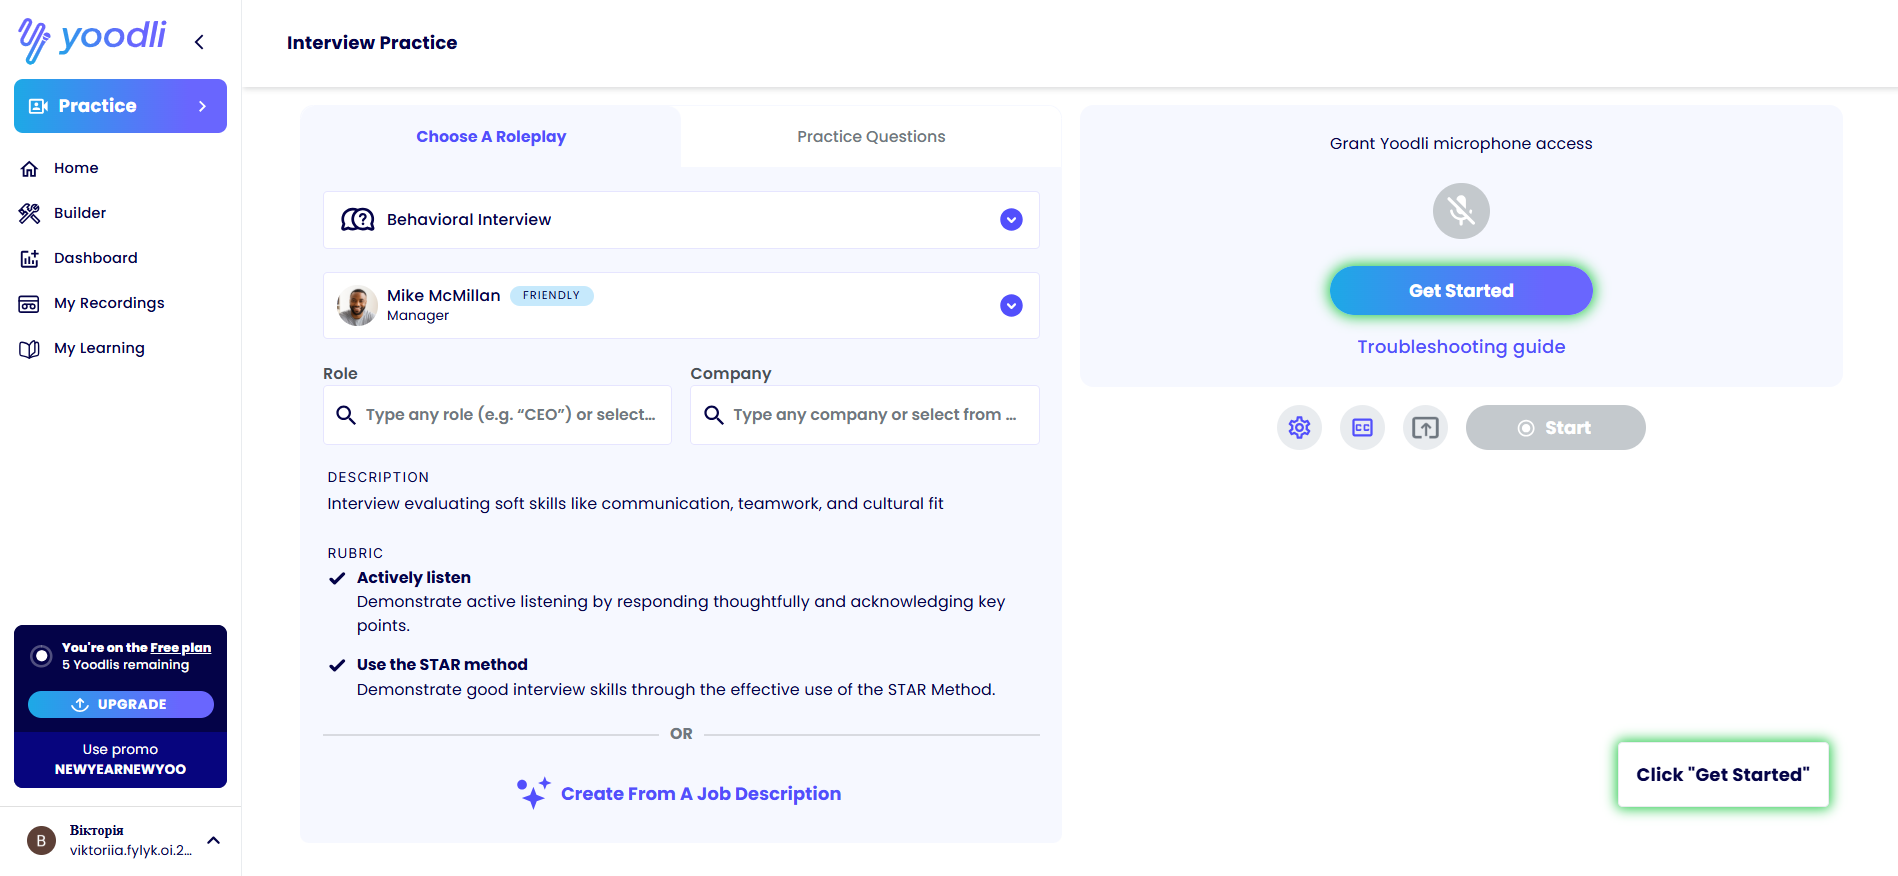
\includegraphics[width=3.5625in,height=5.01888in]{media/media/image6.png}

Рис. Г.1. Схема тристадiйної radix-4 декомпозицiї 16-точкового ШПФ.

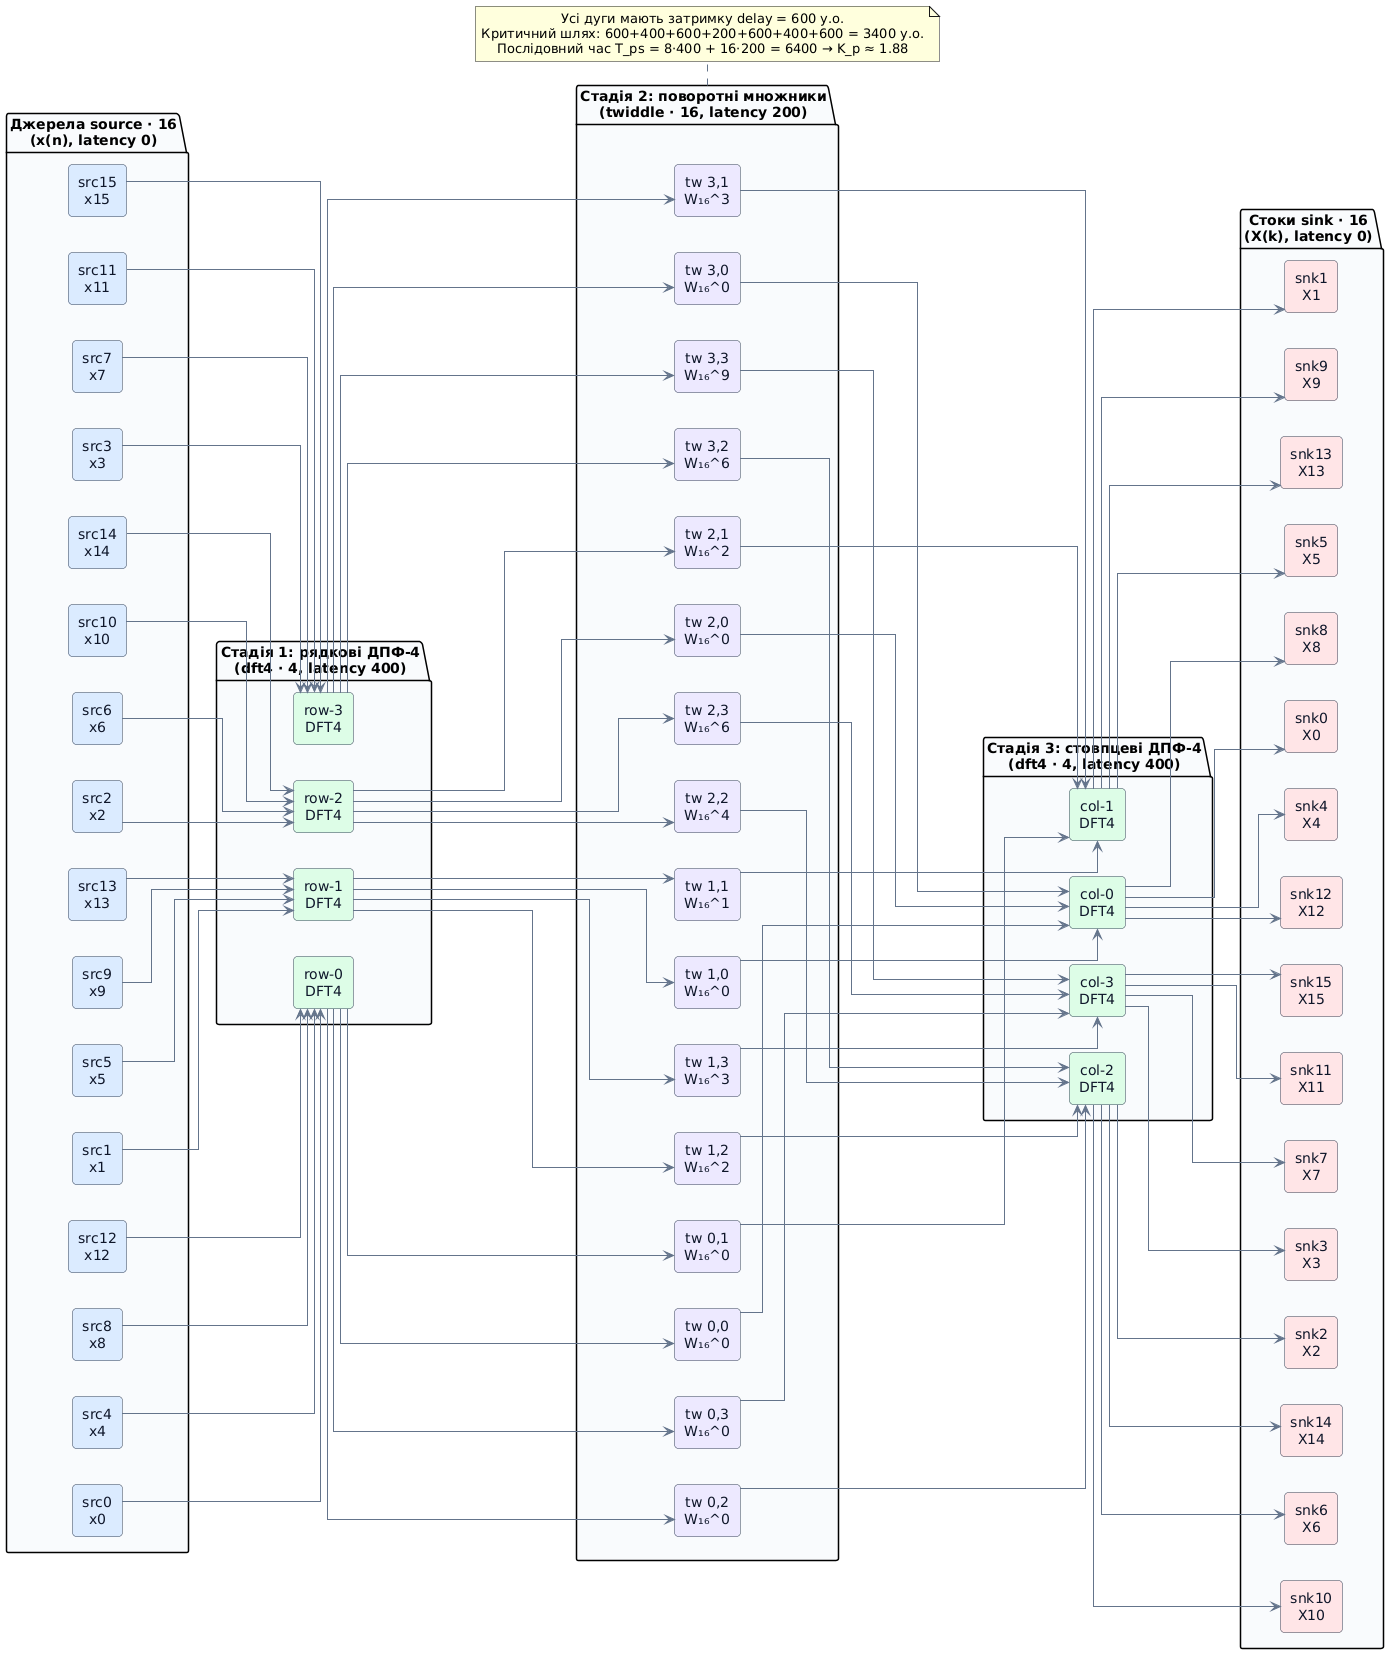
\includegraphics[width=6.49583in,height=7.725in]{media/media/image7.png}

Рис. Г.2. Граф потоку даних обчислювача 16-точкового ШПФ radix-4 4 × 4.

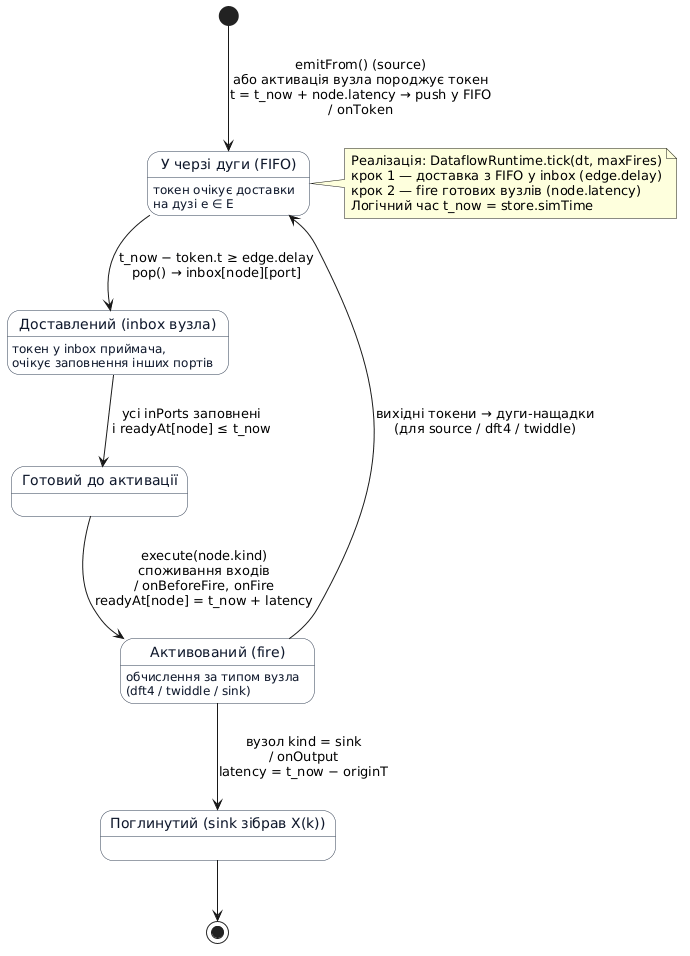
\includegraphics[width=4.0625in,height=5.62861in]{media/media/image8.png}

Рис. Г.3. Життєвий цикл токена у DataflowRuntime.

\textbf{Г.1. Реєстр графічних схем.}

Перелік усіх 9 схем подано у табл. Г.1.

Таблиця Г.1

Реєстр графічних схем БКР

\begin{longtable}[]{@{}
  >{\raggedright\arraybackslash}p{(\linewidth - 8\tabcolsep) * \real{0.0476}}
  >{\raggedright\arraybackslash}p{(\linewidth - 8\tabcolsep) * \real{0.4955}}
  >{\raggedright\arraybackslash}p{(\linewidth - 8\tabcolsep) * \real{0.1797}}
  >{\raggedright\arraybackslash}p{(\linewidth - 8\tabcolsep) * \real{0.1308}}
  >{\raggedright\arraybackslash}p{(\linewidth - 8\tabcolsep) * \real{0.1464}}@{}}
\caption[Реєстр графічних схем БКР]{Реєстр графічних схем
БКР}\tabularnewline
\toprule\noalign{}
\begin{minipage}[b]{\linewidth}\raggedright
№
\end{minipage} & \begin{minipage}[b]{\linewidth}\raggedright
Назва схеми
\end{minipage} & \begin{minipage}[b]{\linewidth}\raggedright
Тип
\end{minipage} & \begin{minipage}[b]{\linewidth}\raggedright
Підрозділ
\end{minipage} & \begin{minipage}[b]{\linewidth}\raggedright
Інструмент
\end{minipage} \\
\midrule\noalign{}
\endfirsthead
\toprule\noalign{}
\begin{minipage}[b]{\linewidth}\raggedright
№
\end{minipage} & \begin{minipage}[b]{\linewidth}\raggedright
Назва схеми
\end{minipage} & \begin{minipage}[b]{\linewidth}\raggedright
Тип
\end{minipage} & \begin{minipage}[b]{\linewidth}\raggedright
Підрозділ
\end{minipage} & \begin{minipage}[b]{\linewidth}\raggedright
Інструмент
\end{minipage} \\
\midrule\noalign{}
\endhead
\bottomrule\noalign{}
\endlastfoot
& Функціональна IDEF0-схема задачі моделювання потокового обчислювача
ШПФ & IDEF0 & рис. 1.1 & PlantUML \\
& Use Case-діаграма симулятора потокового обчислювача ШПФ & UML Use Case
& рис. 1.2 & PlantUML \\
& C4 Context-діаграма веб-симулятора потокового обчислювача ШПФ & C4
Context & рис. 2.1 & PlantUML \\
& Схема тристадійної radix-4 декомпозиції 16-точкового ШПФ &
Алгоритмічна & рис. Г.1 & PlantUML \\
& C4 Container-діаграма архітектури веб-симулятора & C4 Container & рис.
2.3 & PlantUML \\
& Граф потоку даних обчислювача 16-точкового ШПФ radix-4 \(4 \times 4\)
& DFG & рис. Г.2 & PlantUML \\
& Макет інтерфейсу веб-симулятора потокового 16-точкового ШПФ &
Wireframe & рис. 2.5 & PlantUML \\
& Життєвий цикл токена у \passthrough{\lstinline!DataflowRuntime!} &
Sequence & рис. Г.3 & PlantUML \\
& Часова діаграма активацій вузлів DFG при \(N = 16\) & Timing & рис.
4.1 & PlantUML \\
\end{longtable}

\textbf{Г.2. Розташування вихідних описів схем.}

Кожна схема зберігається у каталозі
\passthrough{\lstinline!diagrams!}\passthrough{\lstinline!\_!}\passthrough{\lstinline!output!}\passthrough{\lstinline!/!}
в окремому
\passthrough{\lstinline!.!}\passthrough{\lstinline!txt!}-файлі з ім'ям,
що збігається з підписом рисунка в основному тексті (табл. Г.2).
Відтворити будь-яку схему можна завантаженням відповідного файла на
\passthrough{\lstinline!plantuml!}\passthrough{\lstinline!.!}\passthrough{\lstinline!com!}.

Таблиця Г.2

Відповідність між рисунками і вихідними
\passthrough{\lstinline!.!}\passthrough{\lstinline!txt!}-описами

\begin{longtable}[]{@{}
  >{\raggedright\arraybackslash}p{(\linewidth - 2\tabcolsep) * \real{0.0690}}
  >{\raggedright\arraybackslash}p{(\linewidth - 2\tabcolsep) * \real{0.9310}}@{}}
\caption[Відповідність між рисунками і вихідними
.txt-описами]{Відповідність між рисунками і вихідними
.txt-описами}\tabularnewline
\toprule\noalign{}
\begin{minipage}[b]{\linewidth}\raggedright
Рис.
\end{minipage} & \begin{minipage}[b]{\linewidth}\raggedright
Файл у
\passthrough{\lstinline!diagrams\_output!}\passthrough{\lstinline!/!}
\end{minipage} \\
\midrule\noalign{}
\endfirsthead
\toprule\noalign{}
\begin{minipage}[b]{\linewidth}\raggedright
Рис.
\end{minipage} & \begin{minipage}[b]{\linewidth}\raggedright
Файл у
\passthrough{\lstinline!diagrams\_output!}\passthrough{\lstinline!/!}
\end{minipage} \\
\midrule\noalign{}
\endhead
\bottomrule\noalign{}
\endlastfoot
&
\passthrough{\lstinline!Рис.!}\passthrough{\lstinline! !}\passthrough{\lstinline!1.1!}\passthrough{\lstinline! !}\passthrough{\lstinline!--!}\passthrough{\lstinline! !}\passthrough{\lstinline!Функціональна!}\passthrough{\lstinline! !}\passthrough{\lstinline!IDEF!}\passthrough{\lstinline!0-схема!}\passthrough{\lstinline! !}\passthrough{\lstinline!задачі!}\passthrough{\lstinline! !}\passthrough{\lstinline!моделювання!}\passthrough{\lstinline! !}\passthrough{\lstinline!потокового!}\passthrough{\lstinline! !}\passthrough{\lstinline!обчислювача!}\passthrough{\lstinline! !}\passthrough{\lstinline!ШПФ.!}\passthrough{\lstinline!txt!} \\
&
\passthrough{\lstinline!Рис.!}\passthrough{\lstinline! !}\passthrough{\lstinline!1.2!}\passthrough{\lstinline! !}\passthrough{\lstinline!--!}\passthrough{\lstinline! !}\passthrough{\lstinline!Use!}\passthrough{\lstinline! !}\passthrough{\lstinline!Case!}\passthrough{\lstinline!-діаграма!}\passthrough{\lstinline! !}\passthrough{\lstinline!симулятора!}\passthrough{\lstinline! !}\passthrough{\lstinline!потокового!}\passthrough{\lstinline! !}\passthrough{\lstinline!обчислювача!}\passthrough{\lstinline! !}\passthrough{\lstinline!ШПФ.!}\passthrough{\lstinline!txt!} \\
&
\passthrough{\lstinline!Рис.!}\passthrough{\lstinline! !}\passthrough{\lstinline!2.1!}\passthrough{\lstinline! !}\passthrough{\lstinline!--!}\passthrough{\lstinline! !}\passthrough{\lstinline!C!}\passthrough{\lstinline!4!}\passthrough{\lstinline! !}\passthrough{\lstinline!Context!}\passthrough{\lstinline!-діаграма!}\passthrough{\lstinline! !}\passthrough{\lstinline!веб-симулятора!}\passthrough{\lstinline! !}\passthrough{\lstinline!потокового!}\passthrough{\lstinline! !}\passthrough{\lstinline!обчислювача!}\passthrough{\lstinline! !}\passthrough{\lstinline!ШПФ.!}\passthrough{\lstinline!txt!} \\
&
\passthrough{\lstinline!Рис.!}\passthrough{\lstinline! !}\passthrough{\lstinline!Г.1!}\passthrough{\lstinline! !}\passthrough{\lstinline!--!}\passthrough{\lstinline! !}\passthrough{\lstinline!Схема!}\passthrough{\lstinline! !}\passthrough{\lstinline!тристадійної!}\passthrough{\lstinline! !}\passthrough{\lstinline!radix!}\passthrough{\lstinline!-4!}\passthrough{\lstinline! !}\passthrough{\lstinline!декомпозиції!}\passthrough{\lstinline! !}\passthrough{\lstinline!16-точкового!}\passthrough{\lstinline! !}\passthrough{\lstinline!ШПФ.!}\passthrough{\lstinline!txt!} \\
&
\passthrough{\lstinline!Рис.!}\passthrough{\lstinline! !}\passthrough{\lstinline!2.3!}\passthrough{\lstinline! !}\passthrough{\lstinline!--!}\passthrough{\lstinline! !}\passthrough{\lstinline!C!}\passthrough{\lstinline!4!}\passthrough{\lstinline! !}\passthrough{\lstinline!Container!}\passthrough{\lstinline!-діаграма!}\passthrough{\lstinline! !}\passthrough{\lstinline!архітектури!}\passthrough{\lstinline! !}\passthrough{\lstinline!веб-симулятора.!}\passthrough{\lstinline!txt!} \\
&
\passthrough{\lstinline!Рис.!}\passthrough{\lstinline! !}\passthrough{\lstinline!Г.2!}\passthrough{\lstinline! !}\passthrough{\lstinline!--!}\passthrough{\lstinline! !}\passthrough{\lstinline!Граф!}\passthrough{\lstinline! !}\passthrough{\lstinline!потоку!}\passthrough{\lstinline! !}\passthrough{\lstinline!даних!}\passthrough{\lstinline! !}\passthrough{\lstinline!обчислювача!}\passthrough{\lstinline! !}\passthrough{\lstinline!16-точкового!}\passthrough{\lstinline! !}\passthrough{\lstinline!ШПФ!}\passthrough{\lstinline! !}\passthrough{\lstinline!radix!}\passthrough{\lstinline!-4!}\passthrough{\lstinline! !}\passthrough{\lstinline!4×4.!}\passthrough{\lstinline!txt!} \\
&
\passthrough{\lstinline!Рис.!}\passthrough{\lstinline! !}\passthrough{\lstinline!2.5!}\passthrough{\lstinline! !}\passthrough{\lstinline!--!}\passthrough{\lstinline! !}\passthrough{\lstinline!Макет!}\passthrough{\lstinline! !}\passthrough{\lstinline!інтерфейсу!}\passthrough{\lstinline! !}\passthrough{\lstinline!веб-симулятора!}\passthrough{\lstinline! !}\passthrough{\lstinline!потокового!}\passthrough{\lstinline! !}\passthrough{\lstinline!16-точкового!}\passthrough{\lstinline! !}\passthrough{\lstinline!ШПФ.!}\passthrough{\lstinline!txt!} \\
&
\passthrough{\lstinline!Рис.!}\passthrough{\lstinline! !}\passthrough{\lstinline!Г.3!}\passthrough{\lstinline! !}\passthrough{\lstinline!--!}\passthrough{\lstinline! !}\passthrough{\lstinline!Життєвий!}\passthrough{\lstinline! !}\passthrough{\lstinline!цикл!}\passthrough{\lstinline! !}\passthrough{\lstinline!токена!}\passthrough{\lstinline! !}\passthrough{\lstinline!у!}\passthrough{\lstinline! !}\passthrough{\lstinline!DataflowRuntime!}\passthrough{\lstinline!.!}\passthrough{\lstinline!txt!} \\
&
\passthrough{\lstinline!Рис.!}\passthrough{\lstinline! !}\passthrough{\lstinline!4.1!}\passthrough{\lstinline! !}\passthrough{\lstinline!--!}\passthrough{\lstinline! !}\passthrough{\lstinline!Часова!}\passthrough{\lstinline! !}\passthrough{\lstinline!діаграма!}\passthrough{\lstinline! !}\passthrough{\lstinline!активацій!}\passthrough{\lstinline! !}\passthrough{\lstinline!вузлів!}\passthrough{\lstinline! !}\passthrough{\lstinline!DFG!}\passthrough{\lstinline! !}\passthrough{\lstinline!при!}\passthrough{\lstinline! !}\passthrough{\lstinline!N!}\passthrough{\lstinline!=16.!}\passthrough{\lstinline!txt!} \\
\end{longtable}

Г.3. Короткий опис призначення схем.

\begin{itemize}
\item
  \emph{Рис. 1.1, IDEF0-схема задачі моделювання.} Функціональна
  декомпозиція задачі: вхідний сигнал і параметри моделі перетворюються
  на спектральні відліки, журнал подій та метрики виконання під
  керуванням вимог F1--F9, NF1--NF8 і методичних обмежень. Використана
  для постановки задачі (підрозд. 1.3).
\item
  \emph{Рис. 1.2, Use Case-діаграма.} Прецеденти UC1--UC9 з акторами
  Студент і Викладач; містить відношення
  \passthrough{\lstinline!include!} (UC3 \(\rightarrow\) UC5) та
  \passthrough{\lstinline!extend!} (UC7 \(\rightarrow\) UC3); прецеденти
  UC1 і UC2 -- взаємовиключні альтернативи (підрозд. 1.5).
\item
  \emph{Рис. 2.1, C4 Context-діаграма.} Симулятор як ``чорна скринька'';
  актор -- Користувач; зовнішні сутності -- браузер (runtime) і Local
  Storage браузера (для пресетів). Використана для обґрунтування
  клієнтського SPA-підходу (підрозд. 2.1).
\item
  \emph{Рис. Г.1, схема тристадійної radix-4 декомпозиції.} Логічна
  послідовність стадій:
  \(\text{src} \rightarrow \text{row-DFT}_{4} \rightarrow \text{twiddle} \rightarrow \text{col-DFT}_{4} \rightarrow \text{sink}\).
  Ілюструє математичну модель підрозд. 2.2.
\item
  \emph{Рис. 2.3, C4 Container-діаграма.} Декомпозиція симулятора на 4
  контейнери: \emph{Simulation Core}, \emph{Graph Generator},
  \emph{State Store}, \emph{UI Layer}. Використана у підрозд. 2.3.
\item
  \emph{Рис. Г.2, граф потоку даних (DFG).} Повний граф із 56 вузлів
  чотирьох типів і 64 дуг із однаковим \passthrough{\lstinline!delay!}
  \(= 600\). Зображено п'ять ярусів і всі комутаційні зв'язки відповідно
  до
  \passthrough{\lstinline!generateDFT!}\passthrough{\lstinline!4!}\passthrough{\lstinline!x!}\passthrough{\lstinline!4()!}
  (підрозд. 2.3, Додаток А п. А.5).
\item
  \emph{Рис. 2.5, макет інтерфейсу.} Чотири функціональні зони:
  центральний \passthrough{\lstinline!GraphView!}, верхня панель
  \passthrough{\lstinline!Controls!}, права панель
  \passthrough{\lstinline!SpectrumView!}+\passthrough{\lstinline!Metrics!},
  нижня \passthrough{\lstinline!TerminalOutput!} (підрозд. 2.6).
\item
  \emph{Рис. Г.3, життєвий цикл токена.} Послідовність дій у методі
  \passthrough{\lstinline!tick!}\passthrough{\lstinline!()!}: доставка з
  FIFO-черги \(\rightarrow\) приміщення у
  \passthrough{\lstinline!inbox!} \(\rightarrow\) активація вузла
  \(\rightarrow\) генерація токена виходу \(\rightarrow\) постановка у
  нову чергу (підрозд. 3.3, Додаток А п. А.4).
\item
  \emph{Рис. 4.1, часова діаграма активацій.} Ярусний розклад активацій
  вузлів за реальним графом: \(t = 0,600,1000,1600,1800,2400,2800,3400\)
  у.о.; критичний шлях \(T_{kr} = 3400\) у.о.; коефіцієнт
  \(K_{p} \approx 1,88\) (підрозд. 4.3, Додаток В табл. В.3).
\end{itemize}

\textbf{Г.4. Інші ілюстрації основного тексту.}

Окрім схем, побудованих у PlantUML, основний текст БКР містить рисунок
\emph{Рис. 3.1. Структура директорій проєкту} (підрозд. 3.2; рисунок
текстового характеру, формується безпосередньо у LaTeX). Передбачено
також рисунок \emph{Рис. 4.2. Загальний вигляд інтерфейсу веб-симулятора
під час роботи} (підрозд. 4.5) -- скріншот робочого екрана, виконання
якого описано у п. Б4.

\textbf{Г.5. Відсутність копій публікацій.}

Окремі публікації за темою бакалаврської кваліфікаційної роботи на
момент її подання не виходили. Тому Додаток Д (``Копії власних
публікацій за темою БКР'') не формується. Цей факт зафіксовано також у
Вступі (розділ \emph{Апробація результатів}).

\end{document}
